% Options for packages loaded elsewhere
\PassOptionsToPackage{unicode}{hyperref}
\PassOptionsToPackage{hyphens}{url}
%
\documentclass[
]{article}
\usepackage{amsmath,amssymb}
\usepackage{iftex}
\ifPDFTeX
  \usepackage[T1]{fontenc}
  \usepackage[utf8]{inputenc}
  \usepackage{textcomp} % provide euro and other symbols
\else % if luatex or xetex
  \usepackage{unicode-math} % this also loads fontspec
  \defaultfontfeatures{Scale=MatchLowercase}
  \defaultfontfeatures[\rmfamily]{Ligatures=TeX,Scale=1}
\fi
\usepackage{lmodern}
\ifPDFTeX\else
  % xetex/luatex font selection
\fi
% Use upquote if available, for straight quotes in verbatim environments
\IfFileExists{upquote.sty}{\usepackage{upquote}}{}
\IfFileExists{microtype.sty}{% use microtype if available
  \usepackage[]{microtype}
  \UseMicrotypeSet[protrusion]{basicmath} % disable protrusion for tt fonts
}{}
\makeatletter
\@ifundefined{KOMAClassName}{% if non-KOMA class
  \IfFileExists{parskip.sty}{%
    \usepackage{parskip}
  }{% else
    \setlength{\parindent}{0pt}
    \setlength{\parskip}{6pt plus 2pt minus 1pt}}
}{% if KOMA class
  \KOMAoptions{parskip=half}}
\makeatother
\usepackage{xcolor}
\usepackage[margin=1in]{geometry}
\usepackage{color}
\usepackage{fancyvrb}
\newcommand{\VerbBar}{|}
\newcommand{\VERB}{\Verb[commandchars=\\\{\}]}
\DefineVerbatimEnvironment{Highlighting}{Verbatim}{commandchars=\\\{\}}
% Add ',fontsize=\small' for more characters per line
\usepackage{framed}
\definecolor{shadecolor}{RGB}{248,248,248}
\newenvironment{Shaded}{\begin{snugshade}}{\end{snugshade}}
\newcommand{\AlertTok}[1]{\textcolor[rgb]{0.94,0.16,0.16}{#1}}
\newcommand{\AnnotationTok}[1]{\textcolor[rgb]{0.56,0.35,0.01}{\textbf{\textit{#1}}}}
\newcommand{\AttributeTok}[1]{\textcolor[rgb]{0.13,0.29,0.53}{#1}}
\newcommand{\BaseNTok}[1]{\textcolor[rgb]{0.00,0.00,0.81}{#1}}
\newcommand{\BuiltInTok}[1]{#1}
\newcommand{\CharTok}[1]{\textcolor[rgb]{0.31,0.60,0.02}{#1}}
\newcommand{\CommentTok}[1]{\textcolor[rgb]{0.56,0.35,0.01}{\textit{#1}}}
\newcommand{\CommentVarTok}[1]{\textcolor[rgb]{0.56,0.35,0.01}{\textbf{\textit{#1}}}}
\newcommand{\ConstantTok}[1]{\textcolor[rgb]{0.56,0.35,0.01}{#1}}
\newcommand{\ControlFlowTok}[1]{\textcolor[rgb]{0.13,0.29,0.53}{\textbf{#1}}}
\newcommand{\DataTypeTok}[1]{\textcolor[rgb]{0.13,0.29,0.53}{#1}}
\newcommand{\DecValTok}[1]{\textcolor[rgb]{0.00,0.00,0.81}{#1}}
\newcommand{\DocumentationTok}[1]{\textcolor[rgb]{0.56,0.35,0.01}{\textbf{\textit{#1}}}}
\newcommand{\ErrorTok}[1]{\textcolor[rgb]{0.64,0.00,0.00}{\textbf{#1}}}
\newcommand{\ExtensionTok}[1]{#1}
\newcommand{\FloatTok}[1]{\textcolor[rgb]{0.00,0.00,0.81}{#1}}
\newcommand{\FunctionTok}[1]{\textcolor[rgb]{0.13,0.29,0.53}{\textbf{#1}}}
\newcommand{\ImportTok}[1]{#1}
\newcommand{\InformationTok}[1]{\textcolor[rgb]{0.56,0.35,0.01}{\textbf{\textit{#1}}}}
\newcommand{\KeywordTok}[1]{\textcolor[rgb]{0.13,0.29,0.53}{\textbf{#1}}}
\newcommand{\NormalTok}[1]{#1}
\newcommand{\OperatorTok}[1]{\textcolor[rgb]{0.81,0.36,0.00}{\textbf{#1}}}
\newcommand{\OtherTok}[1]{\textcolor[rgb]{0.56,0.35,0.01}{#1}}
\newcommand{\PreprocessorTok}[1]{\textcolor[rgb]{0.56,0.35,0.01}{\textit{#1}}}
\newcommand{\RegionMarkerTok}[1]{#1}
\newcommand{\SpecialCharTok}[1]{\textcolor[rgb]{0.81,0.36,0.00}{\textbf{#1}}}
\newcommand{\SpecialStringTok}[1]{\textcolor[rgb]{0.31,0.60,0.02}{#1}}
\newcommand{\StringTok}[1]{\textcolor[rgb]{0.31,0.60,0.02}{#1}}
\newcommand{\VariableTok}[1]{\textcolor[rgb]{0.00,0.00,0.00}{#1}}
\newcommand{\VerbatimStringTok}[1]{\textcolor[rgb]{0.31,0.60,0.02}{#1}}
\newcommand{\WarningTok}[1]{\textcolor[rgb]{0.56,0.35,0.01}{\textbf{\textit{#1}}}}
\usepackage{graphicx}
\makeatletter
\def\maxwidth{\ifdim\Gin@nat@width>\linewidth\linewidth\else\Gin@nat@width\fi}
\def\maxheight{\ifdim\Gin@nat@height>\textheight\textheight\else\Gin@nat@height\fi}
\makeatother
% Scale images if necessary, so that they will not overflow the page
% margins by default, and it is still possible to overwrite the defaults
% using explicit options in \includegraphics[width, height, ...]{}
\setkeys{Gin}{width=\maxwidth,height=\maxheight,keepaspectratio}
% Set default figure placement to htbp
\makeatletter
\def\fps@figure{htbp}
\makeatother
\setlength{\emergencystretch}{3em} % prevent overfull lines
\providecommand{\tightlist}{%
  \setlength{\itemsep}{0pt}\setlength{\parskip}{0pt}}
\setcounter{secnumdepth}{-\maxdimen} % remove section numbering
\ifLuaTeX
  \usepackage{selnolig}  % disable illegal ligatures
\fi
\IfFileExists{bookmark.sty}{\usepackage{bookmark}}{\usepackage{hyperref}}
\IfFileExists{xurl.sty}{\usepackage{xurl}}{} % add URL line breaks if available
\urlstyle{same}
\hypersetup{
  pdftitle={Figure4\_v2},
  pdfauthor={Nikita Verheyden},
  hidelinks,
  pdfcreator={LaTeX via pandoc}}

\title{Figure4\_v2}
\author{Nikita Verheyden}
\date{2023-06-13}

\begin{document}
\maketitle

\hypertarget{setup}{%
\section{Setup}\label{setup}}

dir

\begin{Shaded}
\begin{Highlighting}[]
\FunctionTok{setwd}\NormalTok{(}\StringTok{"C:/Users/nikit/Documents/Krueger\_Lab/Publications/miR181\_paper/Figure4"}\NormalTok{)}
\end{Highlighting}
\end{Shaded}

\hypertarget{packages}{%
\subsection{Packages}\label{packages}}

\begin{Shaded}
\begin{Highlighting}[]
\FunctionTok{source}\NormalTok{(}\StringTok{"C:/Users/nikit/Documents/Krueger\_Lab/Publications/miR181\_paper/Supporting\_scripts/themes/theme\_paper.R"}\NormalTok{)}
\FunctionTok{library}\NormalTok{(ggplot2)}
\FunctionTok{library}\NormalTok{(rtracklayer)}
\end{Highlighting}
\end{Shaded}

\begin{verbatim}
## Loading required package: GenomicRanges
\end{verbatim}

\begin{verbatim}
## Loading required package: stats4
\end{verbatim}

\begin{verbatim}
## Loading required package: BiocGenerics
\end{verbatim}

\begin{verbatim}
## 
## Attaching package: 'BiocGenerics'
\end{verbatim}

\begin{verbatim}
## The following objects are masked from 'package:stats':
## 
##     IQR, mad, sd, var, xtabs
\end{verbatim}

\begin{verbatim}
## The following objects are masked from 'package:base':
## 
##     anyDuplicated, aperm, append, as.data.frame, basename, cbind,
##     colnames, dirname, do.call, duplicated, eval, evalq, Filter, Find,
##     get, grep, grepl, intersect, is.unsorted, lapply, Map, mapply,
##     match, mget, order, paste, pmax, pmax.int, pmin, pmin.int,
##     Position, rank, rbind, Reduce, rownames, sapply, setdiff, sort,
##     table, tapply, union, unique, unsplit, which.max, which.min
\end{verbatim}

\begin{verbatim}
## Loading required package: S4Vectors
\end{verbatim}

\begin{verbatim}
## 
## Attaching package: 'S4Vectors'
\end{verbatim}

\begin{verbatim}
## The following object is masked from 'package:utils':
## 
##     findMatches
\end{verbatim}

\begin{verbatim}
## The following objects are masked from 'package:base':
## 
##     expand.grid, I, unname
\end{verbatim}

\begin{verbatim}
## Loading required package: IRanges
\end{verbatim}

\begin{verbatim}
## 
## Attaching package: 'IRanges'
\end{verbatim}

\begin{verbatim}
## The following object is masked from 'package:grDevices':
## 
##     windows
\end{verbatim}

\begin{verbatim}
## Loading required package: GenomeInfoDb
\end{verbatim}

\begin{Shaded}
\begin{Highlighting}[]
\FunctionTok{library}\NormalTok{(dplyr)}
\end{Highlighting}
\end{Shaded}

\begin{verbatim}
## 
## Attaching package: 'dplyr'
\end{verbatim}

\begin{verbatim}
## The following objects are masked from 'package:GenomicRanges':
## 
##     intersect, setdiff, union
\end{verbatim}

\begin{verbatim}
## The following object is masked from 'package:GenomeInfoDb':
## 
##     intersect
\end{verbatim}

\begin{verbatim}
## The following objects are masked from 'package:IRanges':
## 
##     collapse, desc, intersect, setdiff, slice, union
\end{verbatim}

\begin{verbatim}
## The following objects are masked from 'package:S4Vectors':
## 
##     first, intersect, rename, setdiff, setequal, union
\end{verbatim}

\begin{verbatim}
## The following objects are masked from 'package:BiocGenerics':
## 
##     combine, intersect, setdiff, union
\end{verbatim}

\begin{verbatim}
## The following objects are masked from 'package:stats':
## 
##     filter, lag
\end{verbatim}

\begin{verbatim}
## The following objects are masked from 'package:base':
## 
##     intersect, setdiff, setequal, union
\end{verbatim}

\begin{Shaded}
\begin{Highlighting}[]
\FunctionTok{library}\NormalTok{(tibble)}
\FunctionTok{library}\NormalTok{(Rtsne)}
\FunctionTok{library}\NormalTok{(cliProfiler)}
\FunctionTok{library}\NormalTok{(GenomicRanges)}
\FunctionTok{library}\NormalTok{(cowplot)}
\FunctionTok{library}\NormalTok{(eulerr)}
\FunctionTok{library}\NormalTok{(readxl)}
\FunctionTok{library}\NormalTok{(biomaRt)}
\FunctionTok{library}\NormalTok{(writexl)}
\end{Highlighting}
\end{Shaded}

\hypertarget{data}{%
\subsection{Data}\label{data}}

\begin{Shaded}
\begin{Highlighting}[]
\CommentTok{\#Ribo profiling}
\NormalTok{RNA }\OtherTok{\textless{}{-}} \FunctionTok{read.csv}\NormalTok{(}\StringTok{"C:/Users/nikit/Documents/Krueger\_Lab/Publications/miR181\_paper/Figure3/RNA\_masterframe.csv"}\NormalTok{)}
\NormalTok{RPF }\OtherTok{\textless{}{-}} \FunctionTok{read.csv}\NormalTok{(}\StringTok{"C:/Users/nikit/Documents/Krueger\_Lab/Publications/miR181\_paper/Figure3/RPF\_masterframe.csv"}\NormalTok{)}

\CommentTok{\#load the gtf file to compare genes}
\NormalTok{gff23 }\OtherTok{\textless{}{-}} \FunctionTok{import.gff3}\NormalTok{(}\StringTok{"C:/Users/nikit/Documents/Krueger\_Lab/Ribo\_Profiling/run15112022M23/ref\_genome/gencode.vM23.annotation.gff3.gz"}\NormalTok{)}
\NormalTok{gff23path }\OtherTok{\textless{}{-}} \FunctionTok{file.path}\NormalTok{(}\StringTok{"C:/Users/nikit/Documents/Krueger\_Lab/Ribo\_Profiling/run15112022M23/ref\_genome"}\NormalTok{, }\StringTok{"gencode.vM23.annotation.gff3.gz"}\NormalTok{)}

\CommentTok{\#targets}
\NormalTok{larget }\OtherTok{\textless{}{-}} \FunctionTok{readRDS}\NormalTok{(}\StringTok{"C:/Users/nikit/Documents/Krueger\_Lab/Publications/miR181\_paper/Figure4/mir181\_bs\_with\_seeds\_transcripts.rds"}\NormalTok{)}
\NormalTok{largetframe }\OtherTok{\textless{}{-}} \FunctionTok{as.data.frame}\NormalTok{(larget)}
\FunctionTok{table}\NormalTok{(largetframe}\SpecialCharTok{$}\NormalTok{set)}
\end{Highlighting}
\end{Shaded}

\begin{verbatim}
## 
##                 ago_bs_mir181_chi ago_bs_mir181_chi&mir181_enriched 
##                              5725                              1061 
##                   mir181_enriched 
##                              3458
\end{verbatim}

\begin{Shaded}
\begin{Highlighting}[]
\CommentTok{\# largetframe \textless{}{-} largetframe[!(largetframe$set == "ago\_bs\_mir181\_chi"),]}

\NormalTok{largetframe }\OtherTok{\textless{}{-}}\NormalTok{ largetframe }\SpecialCharTok{\%\textgreater{}\%}
  \FunctionTok{subset}\NormalTok{(set }\SpecialCharTok{\%in\%} \FunctionTok{c}\NormalTok{(}\StringTok{"ago\_bs\_mir181\_chi\&mir181\_enriched"}\NormalTok{, }\StringTok{"mir181\_enriched"}\NormalTok{))}


\CommentTok{\# modify dataset to only include working targetsets}

\CommentTok{\#only use miR181\_enriched und both}
\CommentTok{\# largetframe \textless{}{-} largetframe[largetframe$set \%in\% c("mir181\_enriched", "ago\_bs\_mir181\_chi\&mir181\_enriched"),]}


\CommentTok{\#ms}
\CommentTok{\#ms}
\NormalTok{MS }\OtherTok{\textless{}{-}} \FunctionTok{read.csv}\NormalTok{(}\StringTok{"C:/Users/nikit/Documents/Krueger\_Lab/Publications/miR181\_paper/Figure2/MS\_data\_MMU\_02082023.csv"}\NormalTok{ )}

\CommentTok{\#Translational efficiency}
\NormalTok{TE }\OtherTok{\textless{}{-}} \FunctionTok{read.csv}\NormalTok{(}\StringTok{"C:/Users/nikit/Documents/Krueger\_Lab/Publications/miR181\_paper/Supporting\_scripts/deltaTE/TE\_m23\_genesInRNAandRPF.csv"}\NormalTok{)}




\CommentTok{\#MMsat4}
\CommentTok{\# repeat\_masker \textless{}{-} readRDS("C:/Users/nikit/Documents/Krueger\_Lab/Publications/miR181\_paper/Figure2/MMsat4/repeat\_masker.rds")}
\CommentTok{\# MMSAT4 \textless{}{-} repeat\_masker[repeat\_masker$repName == "MMSAT4"]}
\CommentTok{\# MurSatRep1 \textless{}{-} repeat\_masker[repeat\_masker$repName == "MurSatRep1"]}


\CommentTok{\#melina repeats}
\NormalTok{melrep }\OtherTok{\textless{}{-}} \FunctionTok{readRDS}\NormalTok{(}\StringTok{"C:/Users/nikit/Documents/Krueger\_Lab/Publications/miR181\_paper/Figure3/rep\_on\_transcripts.rds"}\NormalTok{)}
\NormalTok{MMSAT4 }\OtherTok{\textless{}{-}}\NormalTok{ melrep[melrep}\SpecialCharTok{$}\NormalTok{repName }\SpecialCharTok{==} \StringTok{"MMSAT4"}\NormalTok{]}
\NormalTok{MurSatRep1 }\OtherTok{\textless{}{-}}\NormalTok{ melrep[melrep}\SpecialCharTok{$}\NormalTok{repName }\SpecialCharTok{==} \StringTok{"MurSatRep1"}\NormalTok{]}
\end{Highlighting}
\end{Shaded}

\hypertarget{colours}{%
\subsection{colours}\label{colours}}

\begin{Shaded}
\begin{Highlighting}[]
\CommentTok{\#colours}
\NormalTok{farbeneg }\OtherTok{\textless{}{-}} \StringTok{"\#b4b4b4"}
\NormalTok{farbe1 }\OtherTok{\textless{}{-}} \StringTok{"\#0073C2FF"}
\NormalTok{farbe2 }\OtherTok{\textless{}{-}} \StringTok{"\#EFC000FF"}
\NormalTok{farbe3 }\OtherTok{\textless{}{-}} \StringTok{"\#CD534CFF"}
\NormalTok{farbe4 }\OtherTok{\textless{}{-}} \StringTok{"\#7AA6DCFF"}
\NormalTok{farbe5 }\OtherTok{\textless{}{-}} \StringTok{"\#868686FF"}
\NormalTok{farbe6 }\OtherTok{\textless{}{-}} \StringTok{"\#003C67FF"}
\NormalTok{farbe7 }\OtherTok{\textless{}{-}} \StringTok{"\#8F7700FF"}
\NormalTok{farbe8 }\OtherTok{\textless{}{-}} \StringTok{"\#3B3B3BFF"}
\NormalTok{farbe9 }\OtherTok{\textless{}{-}} \StringTok{"\#A73030FF"}
\NormalTok{farbe10 }\OtherTok{\textless{}{-}} \StringTok{"\#4A6990FF"}
\NormalTok{farbe11 }\OtherTok{\textless{}{-}} \StringTok{"\#FF6F00FF"}
\NormalTok{farbe12 }\OtherTok{\textless{}{-}} \StringTok{"\#C71000FF"}
\NormalTok{farbe13 }\OtherTok{\textless{}{-}} \StringTok{"\#008EA0FF"}
\NormalTok{farbe14 }\OtherTok{\textless{}{-}} \StringTok{"\#8A4198FF"}
\NormalTok{farbe15 }\OtherTok{\textless{}{-}} \StringTok{"\#5A9599FF"}
\NormalTok{farbe16 }\OtherTok{\textless{}{-}} \StringTok{"\#FF6348FF"}
  
\NormalTok{RNApcol }\OtherTok{\textless{}{-}} \StringTok{"\#b56504"}
\NormalTok{RNAncol }\OtherTok{\textless{}{-}} \StringTok{"\#027d73"}
\NormalTok{RPFpcol }\OtherTok{\textless{}{-}} \StringTok{"\#c4c404"}
\NormalTok{RPFncol }\OtherTok{\textless{}{-}} \StringTok{"\#8d0391"}
\end{Highlighting}
\end{Shaded}

\hypertarget{axis-limits}{%
\subsection{axis limits}\label{axis-limits}}

\begin{Shaded}
\begin{Highlighting}[]
\NormalTok{xlim }\OtherTok{\textless{}{-}} \FloatTok{0.5}
\NormalTok{zoomfac }\OtherTok{\textless{}{-}} \FloatTok{0.45}
\end{Highlighting}
\end{Shaded}

\hypertarget{number-of-binding-sites}{%
\subsection{number of binding sites}\label{number-of-binding-sites}}

\begin{Shaded}
\begin{Highlighting}[]
\NormalTok{bsnum }\OtherTok{\textless{}{-}} \FunctionTok{as.data.frame}\NormalTok{(}\FunctionTok{table}\NormalTok{(largetframe}\SpecialCharTok{$}\NormalTok{geneName))}
\FunctionTok{colnames}\NormalTok{(bsnum) }\OtherTok{\textless{}{-}} \FunctionTok{c}\NormalTok{(}\StringTok{"gene\_symbol"}\NormalTok{, }\StringTok{"BS\_number"}\NormalTok{)}
\end{Highlighting}
\end{Shaded}

\hypertarget{wobble-plot}{%
\section{wobble plot}\label{wobble-plot}}

\hypertarget{ecdf}{%
\subsection{ecdf}\label{ecdf}}

\begin{Shaded}
\begin{Highlighting}[]
\CommentTok{\#RNA}
\NormalTok{RNA}\SpecialCharTok{$}\NormalTok{wobble }\OtherTok{\textless{}{-}} \StringTok{"Non{-}target"}
\NormalTok{RNA}\SpecialCharTok{$}\NormalTok{wobble[RNA}\SpecialCharTok{$}\NormalTok{gene\_symbol }\SpecialCharTok{\%in\%}\NormalTok{ largetframe[}\FunctionTok{is.na}\NormalTok{(largetframe}\SpecialCharTok{$}\NormalTok{first\_seed\_200down.wobble) ,}\StringTok{"geneName"}\NormalTok{]] }\OtherTok{\textless{}{-}} \StringTok{"No seed"}
\NormalTok{RNA}\SpecialCharTok{$}\NormalTok{wobble[RNA}\SpecialCharTok{$}\NormalTok{gene\_symbol }\SpecialCharTok{\%in\%}\NormalTok{ largetframe[largetframe}\SpecialCharTok{$}\NormalTok{first\_seed\_200down.wobble }\SpecialCharTok{==} \ConstantTok{FALSE}\NormalTok{ ,}\StringTok{"geneName"}\NormalTok{]] }\OtherTok{\textless{}{-}} \StringTok{"Canonical"}
\NormalTok{RNA}\SpecialCharTok{$}\NormalTok{wobble[RNA}\SpecialCharTok{$}\NormalTok{gene\_symbol }\SpecialCharTok{\%in\%}\NormalTok{ largetframe[largetframe}\SpecialCharTok{$}\NormalTok{first\_seed\_200down.wobble }\SpecialCharTok{==} \ConstantTok{TRUE}\NormalTok{ ,}\StringTok{"geneName"}\NormalTok{]] }\OtherTok{\textless{}{-}} \StringTok{"Non{-}Canonical"}
\NormalTok{RNA}\SpecialCharTok{$}\NormalTok{wobble[RNA}\SpecialCharTok{$}\NormalTok{gene\_symbol }\SpecialCharTok{\%in\%}\NormalTok{ bsnum[bsnum}\SpecialCharTok{$}\NormalTok{BS\_number }\SpecialCharTok{\textgreater{}} \DecValTok{1}\NormalTok{, }\StringTok{"gene\_symbol"}\NormalTok{]] }\OtherTok{\textless{}{-}} \StringTok{"Multiple"}
\CommentTok{\#RPF}
\NormalTok{RPF}\SpecialCharTok{$}\NormalTok{wobble }\OtherTok{\textless{}{-}} \StringTok{"Non{-}target"}
\NormalTok{RPF}\SpecialCharTok{$}\NormalTok{wobble[RPF}\SpecialCharTok{$}\NormalTok{gene\_symbol }\SpecialCharTok{\%in\%}\NormalTok{ largetframe[}\FunctionTok{is.na}\NormalTok{(largetframe}\SpecialCharTok{$}\NormalTok{first\_seed\_200down.wobble) ,}\StringTok{"geneName"}\NormalTok{]] }\OtherTok{\textless{}{-}} \StringTok{"No seed"}
\NormalTok{RPF}\SpecialCharTok{$}\NormalTok{wobble[RPF}\SpecialCharTok{$}\NormalTok{gene\_symbol }\SpecialCharTok{\%in\%}\NormalTok{ largetframe[largetframe}\SpecialCharTok{$}\NormalTok{first\_seed\_200down.wobble }\SpecialCharTok{==} \ConstantTok{FALSE}\NormalTok{ ,}\StringTok{"geneName"}\NormalTok{]] }\OtherTok{\textless{}{-}} \StringTok{"Canonical"}
\NormalTok{RPF}\SpecialCharTok{$}\NormalTok{wobble[RPF}\SpecialCharTok{$}\NormalTok{gene\_symbol }\SpecialCharTok{\%in\%}\NormalTok{ largetframe[largetframe}\SpecialCharTok{$}\NormalTok{first\_seed\_200down.wobble }\SpecialCharTok{==} \ConstantTok{TRUE}\NormalTok{ ,}\StringTok{"geneName"}\NormalTok{]] }\OtherTok{\textless{}{-}} \StringTok{"Non{-}Canonical"}
\NormalTok{RPF}\SpecialCharTok{$}\NormalTok{wobble[RPF}\SpecialCharTok{$}\NormalTok{gene\_symbol }\SpecialCharTok{\%in\%}\NormalTok{ bsnum[bsnum}\SpecialCharTok{$}\NormalTok{BS\_number }\SpecialCharTok{\textgreater{}} \DecValTok{1}\NormalTok{, }\StringTok{"gene\_symbol"}\NormalTok{]] }\OtherTok{\textless{}{-}} \StringTok{"Multiple"}

\CommentTok{\#MS}
\NormalTok{MS}\SpecialCharTok{$}\NormalTok{wobble }\OtherTok{\textless{}{-}} \StringTok{"Non{-}target"}
\NormalTok{MS}\SpecialCharTok{$}\NormalTok{wobble[MS}\SpecialCharTok{$}\NormalTok{gene\_symbol }\SpecialCharTok{\%in\%}\NormalTok{ largetframe[}\FunctionTok{is.na}\NormalTok{(largetframe}\SpecialCharTok{$}\NormalTok{first\_seed\_200down.wobble) ,}\StringTok{"geneName"}\NormalTok{]] }\OtherTok{\textless{}{-}} \StringTok{"No seed"}
\NormalTok{MS}\SpecialCharTok{$}\NormalTok{wobble[MS}\SpecialCharTok{$}\NormalTok{gene\_symbol }\SpecialCharTok{\%in\%}\NormalTok{ largetframe[largetframe}\SpecialCharTok{$}\NormalTok{first\_seed\_200down.wobble }\SpecialCharTok{==} \ConstantTok{FALSE}\NormalTok{ ,}\StringTok{"geneName"}\NormalTok{]] }\OtherTok{\textless{}{-}} \StringTok{"Canonical"}
\NormalTok{MS}\SpecialCharTok{$}\NormalTok{wobble[MS}\SpecialCharTok{$}\NormalTok{gene\_symbol }\SpecialCharTok{\%in\%}\NormalTok{ largetframe[largetframe}\SpecialCharTok{$}\NormalTok{first\_seed\_200down.wobble }\SpecialCharTok{==} \ConstantTok{TRUE}\NormalTok{ ,}\StringTok{"geneName"}\NormalTok{]] }\OtherTok{\textless{}{-}} \StringTok{"Non{-}Canonical"}
\NormalTok{MS}\SpecialCharTok{$}\NormalTok{wobble[MS}\SpecialCharTok{$}\NormalTok{gene\_symbol }\SpecialCharTok{\%in\%}\NormalTok{ bsnum[bsnum}\SpecialCharTok{$}\NormalTok{BS\_number }\SpecialCharTok{\textgreater{}} \DecValTok{1}\NormalTok{, }\StringTok{"gene\_symbol"}\NormalTok{]] }\OtherTok{\textless{}{-}} \StringTok{"Multiple"}

\CommentTok{\#TE}
\NormalTok{TE}\SpecialCharTok{$}\NormalTok{wobble }\OtherTok{\textless{}{-}} \StringTok{"Non{-}target"}
\NormalTok{TE}\SpecialCharTok{$}\NormalTok{wobble[TE}\SpecialCharTok{$}\NormalTok{gene\_symbol }\SpecialCharTok{\%in\%}\NormalTok{ largetframe[}\FunctionTok{is.na}\NormalTok{(largetframe}\SpecialCharTok{$}\NormalTok{first\_seed\_200down.wobble) ,}\StringTok{"geneName"}\NormalTok{]] }\OtherTok{\textless{}{-}} \StringTok{"No seed"}
\NormalTok{TE}\SpecialCharTok{$}\NormalTok{wobble[TE}\SpecialCharTok{$}\NormalTok{gene\_symbol }\SpecialCharTok{\%in\%}\NormalTok{ largetframe[largetframe}\SpecialCharTok{$}\NormalTok{first\_seed\_200down.wobble }\SpecialCharTok{==} \ConstantTok{FALSE}\NormalTok{ ,}\StringTok{"geneName"}\NormalTok{]] }\OtherTok{\textless{}{-}} \StringTok{"Canonical"}
\NormalTok{TE}\SpecialCharTok{$}\NormalTok{wobble[TE}\SpecialCharTok{$}\NormalTok{gene\_symbol }\SpecialCharTok{\%in\%}\NormalTok{ largetframe[largetframe}\SpecialCharTok{$}\NormalTok{first\_seed\_200down.wobble }\SpecialCharTok{==} \ConstantTok{TRUE}\NormalTok{ ,}\StringTok{"geneName"}\NormalTok{]] }\OtherTok{\textless{}{-}} \StringTok{"Non{-}Canonical"}
\NormalTok{TE}\SpecialCharTok{$}\NormalTok{wobble[TE}\SpecialCharTok{$}\NormalTok{gene\_symbol }\SpecialCharTok{\%in\%}\NormalTok{ bsnum[bsnum}\SpecialCharTok{$}\NormalTok{BS\_number }\SpecialCharTok{\textgreater{}} \DecValTok{1}\NormalTok{, }\StringTok{"gene\_symbol"}\NormalTok{]] }\OtherTok{\textless{}{-}} \StringTok{"Multiple"}

\CommentTok{\#ECDF}

\CommentTok{\#RNA}
\NormalTok{wobbleecdfRNA }\OtherTok{\textless{}{-}} \FunctionTok{ggplot}\NormalTok{(RNA, }\FunctionTok{aes}\NormalTok{(}\FunctionTok{as.numeric}\NormalTok{(log2FoldChange), }\AttributeTok{colour=}\FunctionTok{factor}\NormalTok{(wobble, }\AttributeTok{levels =} \FunctionTok{c}\NormalTok{(}\StringTok{"Non{-}target"}\NormalTok{, }\StringTok{"No seed"}\NormalTok{, }\StringTok{"Canonical"}\NormalTok{, }\StringTok{"Non{-}Canonical"}\NormalTok{, }\StringTok{"Multiple"}\NormalTok{)))) }\SpecialCharTok{+} 
  \FunctionTok{stat\_ecdf}\NormalTok{(}\AttributeTok{geom=}\StringTok{"step"}\NormalTok{, }\AttributeTok{linewidth=}\DecValTok{2}\NormalTok{) }\SpecialCharTok{+}
  \FunctionTok{geom\_vline}\NormalTok{(}\AttributeTok{xintercept =} \DecValTok{0}\NormalTok{, }\AttributeTok{linewidth=}\DecValTok{1}\NormalTok{, }\AttributeTok{linetype=}\StringTok{"dashed"}\NormalTok{, }\AttributeTok{colour=}\NormalTok{farbeneg) }\SpecialCharTok{+}
  \FunctionTok{scale\_colour\_manual}\NormalTok{(}\AttributeTok{values =} \FunctionTok{c}\NormalTok{(}\StringTok{"black"}\NormalTok{, farbeneg, farbe1, farbe2, farbe3)) }\SpecialCharTok{+}
  \FunctionTok{coord\_cartesian}\NormalTok{(}\AttributeTok{xlim =} \FunctionTok{c}\NormalTok{(}\SpecialCharTok{{-}}\NormalTok{xlim, xlim)) }\SpecialCharTok{+} 
  \FunctionTok{theme\_paper}\NormalTok{() }\SpecialCharTok{+}
  \FunctionTok{scale\_y\_continuous}\NormalTok{(}\StringTok{"Cumulative density"}\NormalTok{) }\SpecialCharTok{+} \FunctionTok{scale\_x\_continuous}\NormalTok{(}\StringTok{"log2FoldChange KO vs WT"}\NormalTok{) }\SpecialCharTok{+}
  \FunctionTok{ggtitle}\NormalTok{(}\StringTok{"Target genes RNAseq"}\NormalTok{)}
\end{Highlighting}
\end{Shaded}

\begin{verbatim}
## Warning: The `size` argument of `element_line()` is deprecated as of ggplot2 3.4.0.
## i Please use the `linewidth` argument instead.
## This warning is displayed once every 8 hours.
## Call `lifecycle::last_lifecycle_warnings()` to see where this warning was
## generated.
\end{verbatim}

\begin{Shaded}
\begin{Highlighting}[]
\NormalTok{wobbleecdfRNA}
\end{Highlighting}
\end{Shaded}

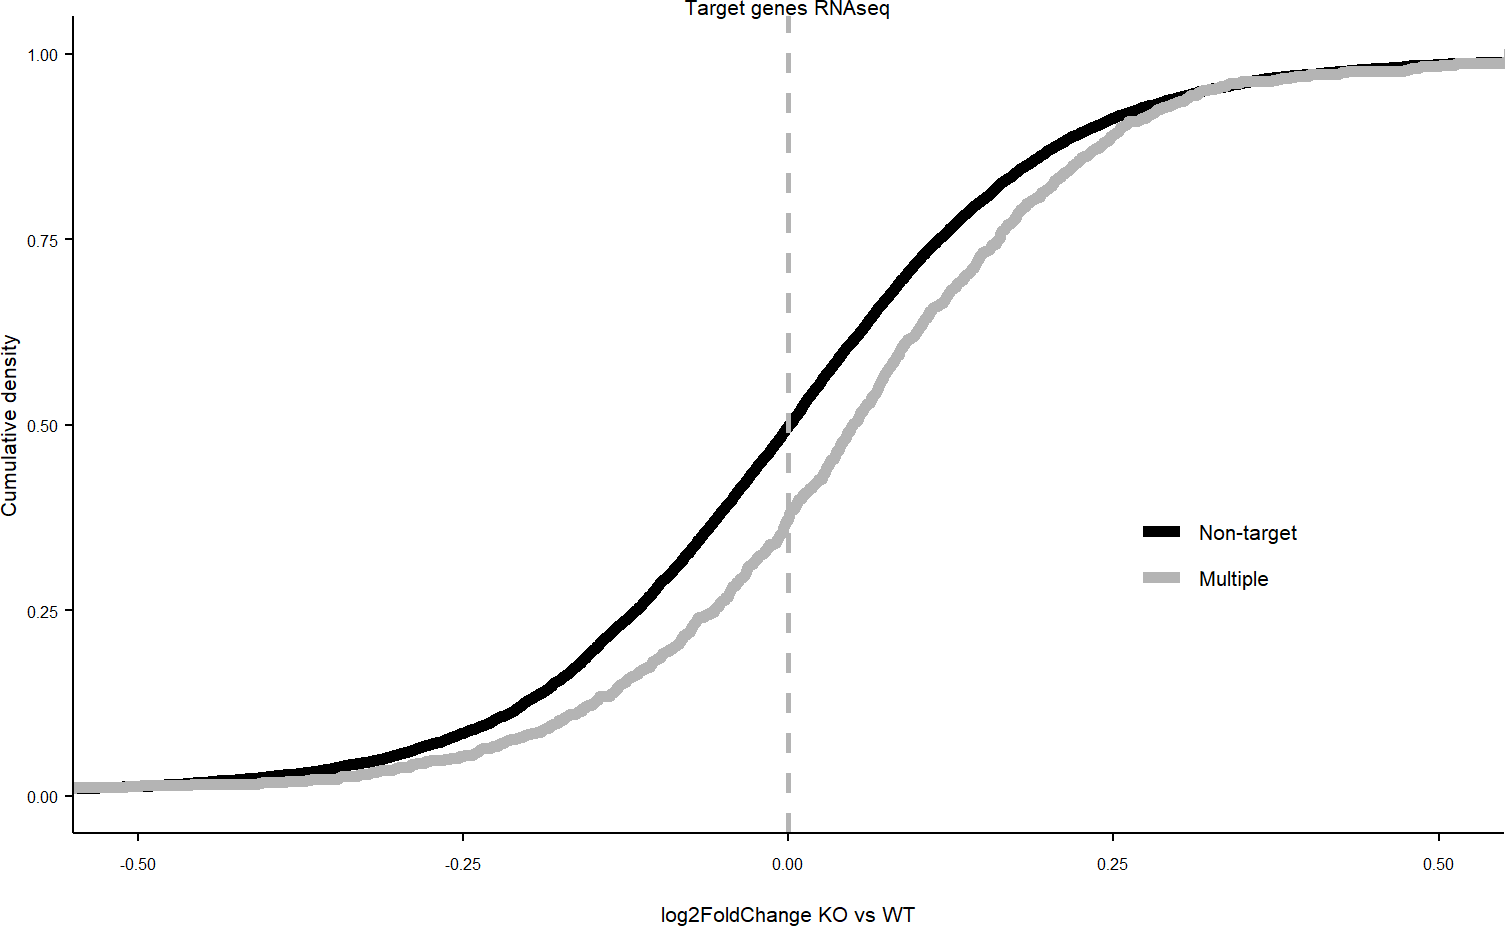
\includegraphics{Fig4_2_files/figure-latex/wobbleecdf-1.pdf}

\begin{Shaded}
\begin{Highlighting}[]
\CommentTok{\#zoom}
\NormalTok{wobbleecdfRNAZ }\OtherTok{\textless{}{-}} \FunctionTok{ggplot}\NormalTok{(RNA, }\FunctionTok{aes}\NormalTok{(}\FunctionTok{as.numeric}\NormalTok{(log2FoldChange), }\AttributeTok{colour=}\FunctionTok{factor}\NormalTok{(wobble, }\AttributeTok{levels =} \FunctionTok{c}\NormalTok{(}\StringTok{"Non{-}target"}\NormalTok{, }\StringTok{"No seed"}\NormalTok{, }\StringTok{"Canonical"}\NormalTok{, }\StringTok{"Non{-}Canonical"}\NormalTok{, }\StringTok{"Multiple"}\NormalTok{)))) }\SpecialCharTok{+} 
  \FunctionTok{stat\_ecdf}\NormalTok{(}\AttributeTok{geom=}\StringTok{"step"}\NormalTok{, }\AttributeTok{linewidth=}\DecValTok{2}\SpecialCharTok{*}\NormalTok{zoomfac) }\SpecialCharTok{+}
  \FunctionTok{geom\_vline}\NormalTok{(}\AttributeTok{xintercept =} \DecValTok{0}\NormalTok{, }\AttributeTok{linewidth=}\DecValTok{1}\SpecialCharTok{*}\NormalTok{zoomfac, }\AttributeTok{linetype=}\StringTok{"dashed"}\NormalTok{, }\AttributeTok{colour=}\NormalTok{farbeneg) }\SpecialCharTok{+}
  \FunctionTok{scale\_colour\_manual}\NormalTok{(}\AttributeTok{values =} \FunctionTok{c}\NormalTok{(}\StringTok{"black"}\NormalTok{, farbeneg, farbe1, farbe2, farbe3)) }\SpecialCharTok{+}
  \FunctionTok{coord\_cartesian}\NormalTok{(}\AttributeTok{xlim =} \FunctionTok{c}\NormalTok{(}\SpecialCharTok{{-}}\NormalTok{(xlim}\SpecialCharTok{/}\DecValTok{8}\NormalTok{), (xlim}\SpecialCharTok{/}\DecValTok{8}\NormalTok{)), }\AttributeTok{ylim =} \FunctionTok{c}\NormalTok{(}\FloatTok{0.5}\DecValTok{{-}1}\SpecialCharTok{/}\DecValTok{16}\NormalTok{, }\FloatTok{0.5}\SpecialCharTok{+}\DecValTok{1}\SpecialCharTok{/}\DecValTok{16}\NormalTok{)) }\SpecialCharTok{+} 
  \FunctionTok{theme\_bw}\NormalTok{() }\SpecialCharTok{+}
  \FunctionTok{theme}\NormalTok{(}\AttributeTok{legend.position =} \StringTok{"none"}\NormalTok{, }\AttributeTok{axis.text =} \FunctionTok{element\_blank}\NormalTok{(), }\AttributeTok{panel.grid =} \FunctionTok{element\_blank}\NormalTok{(),}
        \AttributeTok{panel.background =} \FunctionTok{element\_rect}\NormalTok{(}\AttributeTok{fill=}\StringTok{\textquotesingle{}transparent\textquotesingle{}}\NormalTok{), }\CommentTok{\#transparent panel bg}
        \AttributeTok{plot.background =} \FunctionTok{element\_rect}\NormalTok{(}\AttributeTok{fill=}\StringTok{\textquotesingle{}transparent\textquotesingle{}}\NormalTok{, }\AttributeTok{color=}\ConstantTok{NA}\NormalTok{)) }\SpecialCharTok{+}
  \FunctionTok{scale\_y\_continuous}\NormalTok{(}\StringTok{""}\NormalTok{) }\SpecialCharTok{+} \FunctionTok{scale\_x\_continuous}\NormalTok{(}\StringTok{""}\NormalTok{)}


\NormalTok{wobbleecdfRNAZ}
\end{Highlighting}
\end{Shaded}

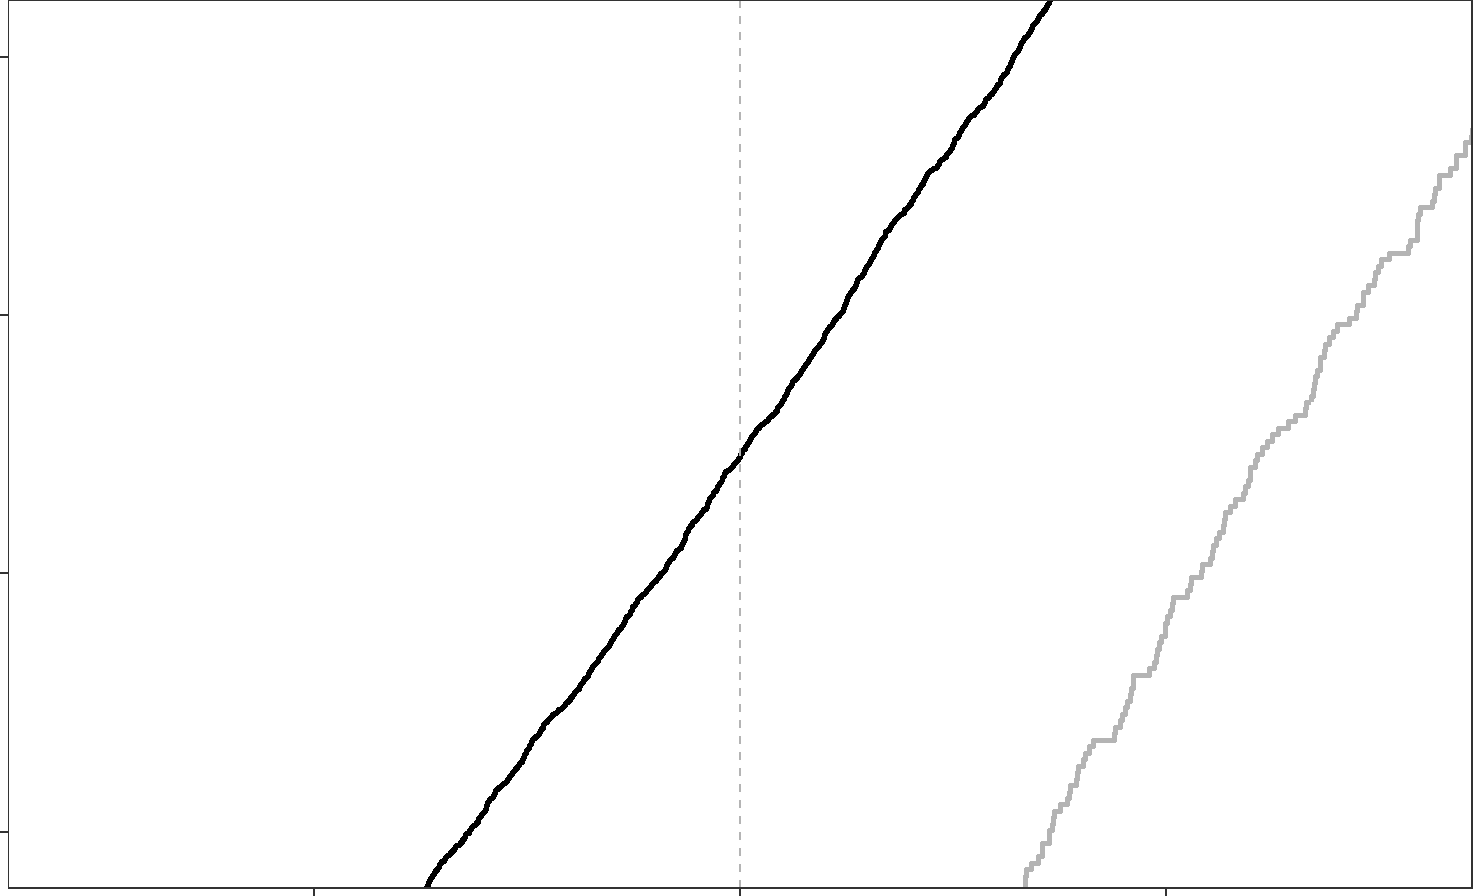
\includegraphics{Fig4_2_files/figure-latex/wobbleecdf-2.pdf}

\begin{Shaded}
\begin{Highlighting}[]
\CommentTok{\#RPF}
\NormalTok{wobbleecdfRPF }\OtherTok{\textless{}{-}} \FunctionTok{ggplot}\NormalTok{(RPF, }\FunctionTok{aes}\NormalTok{(}\FunctionTok{as.numeric}\NormalTok{(log2FoldChange), }\AttributeTok{colour=}\FunctionTok{factor}\NormalTok{(wobble, }\AttributeTok{levels =} \FunctionTok{c}\NormalTok{(}\StringTok{"Non{-}target"}\NormalTok{, }\StringTok{"No seed"}\NormalTok{, }\StringTok{"Canonical"}\NormalTok{, }\StringTok{"Non{-}Canonical"}\NormalTok{, }\StringTok{"Multiple"}\NormalTok{)))) }\SpecialCharTok{+} 
  \FunctionTok{stat\_ecdf}\NormalTok{(}\AttributeTok{geom=}\StringTok{"step"}\NormalTok{, }\AttributeTok{linewidth=}\DecValTok{2}\NormalTok{) }\SpecialCharTok{+}
  \FunctionTok{geom\_vline}\NormalTok{(}\AttributeTok{xintercept =} \DecValTok{0}\NormalTok{, }\AttributeTok{linewidth=}\DecValTok{1}\NormalTok{, }\AttributeTok{linetype=}\StringTok{"dashed"}\NormalTok{, }\AttributeTok{colour=}\NormalTok{farbeneg) }\SpecialCharTok{+}
  \FunctionTok{scale\_colour\_manual}\NormalTok{(}\AttributeTok{values =} \FunctionTok{c}\NormalTok{(}\StringTok{"black"}\NormalTok{, farbeneg, farbe1, farbe2, farbe3)) }\SpecialCharTok{+}
  \FunctionTok{coord\_cartesian}\NormalTok{(}\AttributeTok{xlim =} \FunctionTok{c}\NormalTok{(}\SpecialCharTok{{-}}\NormalTok{xlim, xlim)) }\SpecialCharTok{+} 
  \FunctionTok{theme\_paper}\NormalTok{() }\SpecialCharTok{+}
  \FunctionTok{scale\_y\_continuous}\NormalTok{(}\StringTok{"Cumulative density"}\NormalTok{) }\SpecialCharTok{+} \FunctionTok{scale\_x\_continuous}\NormalTok{(}\StringTok{"log2FoldChange KO vs WT"}\NormalTok{) }\SpecialCharTok{+}
  \FunctionTok{ggtitle}\NormalTok{(}\StringTok{"Target genes ribosome profiling"}\NormalTok{)}

\NormalTok{wobbleecdfRPF}
\end{Highlighting}
\end{Shaded}

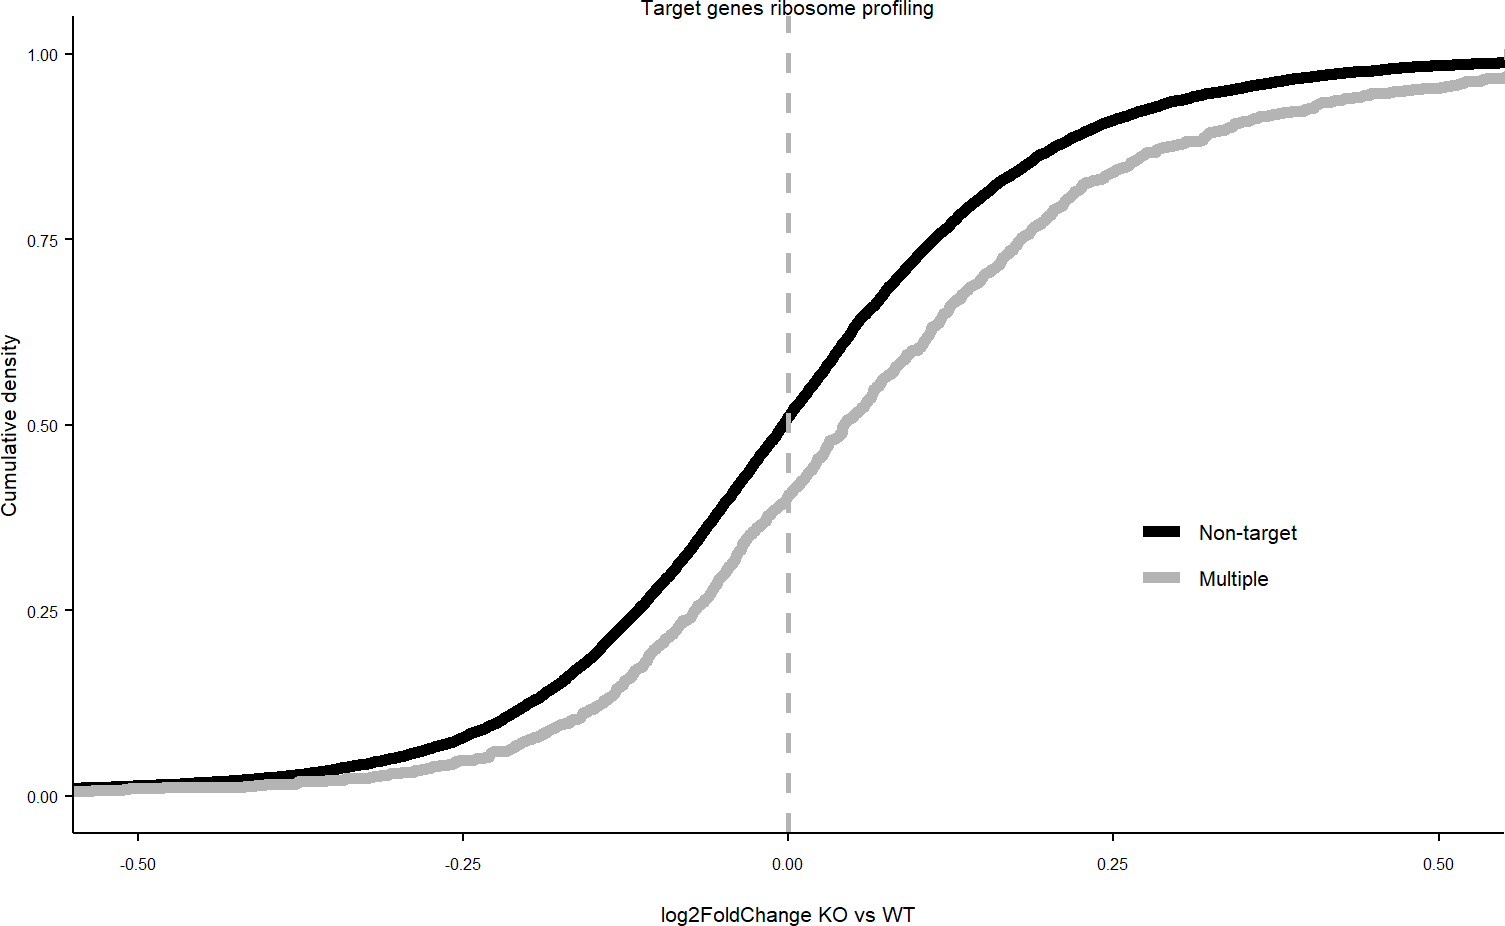
\includegraphics{Fig4_2_files/figure-latex/wobbleecdf-3.pdf}

\begin{Shaded}
\begin{Highlighting}[]
\CommentTok{\#zoom}
\NormalTok{wobbleecdfRPFZ }\OtherTok{\textless{}{-}} \FunctionTok{ggplot}\NormalTok{(RPF, }\FunctionTok{aes}\NormalTok{(}\FunctionTok{as.numeric}\NormalTok{(log2FoldChange), }\AttributeTok{colour=}\FunctionTok{factor}\NormalTok{(wobble, }\AttributeTok{levels =} \FunctionTok{c}\NormalTok{(}\StringTok{"Non{-}target"}\NormalTok{, }\StringTok{"No seed"}\NormalTok{, }\StringTok{"Canonical"}\NormalTok{, }\StringTok{"Non{-}Canonical"}\NormalTok{, }\StringTok{"Multiple"}\NormalTok{)))) }\SpecialCharTok{+} 
  \FunctionTok{stat\_ecdf}\NormalTok{(}\AttributeTok{geom=}\StringTok{"step"}\NormalTok{, }\AttributeTok{linewidth=}\DecValTok{2}\SpecialCharTok{*}\NormalTok{zoomfac) }\SpecialCharTok{+}
  \FunctionTok{geom\_vline}\NormalTok{(}\AttributeTok{xintercept =} \DecValTok{0}\NormalTok{, }\AttributeTok{linewidth=}\DecValTok{1}\SpecialCharTok{*}\NormalTok{zoomfac, }\AttributeTok{linetype=}\StringTok{"dashed"}\NormalTok{, }\AttributeTok{colour=}\NormalTok{farbeneg) }\SpecialCharTok{+}
  \FunctionTok{scale\_colour\_manual}\NormalTok{(}\AttributeTok{values =} \FunctionTok{c}\NormalTok{(}\StringTok{"black"}\NormalTok{, farbeneg, farbe1, farbe2, farbe3)) }\SpecialCharTok{+}
  \FunctionTok{coord\_cartesian}\NormalTok{(}\AttributeTok{xlim =} \FunctionTok{c}\NormalTok{(}\SpecialCharTok{{-}}\NormalTok{(xlim}\SpecialCharTok{/}\DecValTok{8}\NormalTok{), (xlim}\SpecialCharTok{/}\DecValTok{8}\NormalTok{)), }\AttributeTok{ylim =} \FunctionTok{c}\NormalTok{(}\FloatTok{0.5}\DecValTok{{-}1}\SpecialCharTok{/}\DecValTok{16}\NormalTok{, }\FloatTok{0.5}\SpecialCharTok{+}\DecValTok{1}\SpecialCharTok{/}\DecValTok{16}\NormalTok{)) }\SpecialCharTok{+} 
  \FunctionTok{theme\_bw}\NormalTok{() }\SpecialCharTok{+}
  \FunctionTok{theme}\NormalTok{(}\AttributeTok{legend.position =} \StringTok{"none"}\NormalTok{, }\AttributeTok{axis.text =} \FunctionTok{element\_blank}\NormalTok{(), }\AttributeTok{panel.grid =} \FunctionTok{element\_blank}\NormalTok{(),}
        \AttributeTok{panel.background =} \FunctionTok{element\_rect}\NormalTok{(}\AttributeTok{fill=}\StringTok{\textquotesingle{}transparent\textquotesingle{}}\NormalTok{), }\CommentTok{\#transparent panel bg}
        \AttributeTok{plot.background =} \FunctionTok{element\_rect}\NormalTok{(}\AttributeTok{fill=}\StringTok{\textquotesingle{}transparent\textquotesingle{}}\NormalTok{, }\AttributeTok{color=}\ConstantTok{NA}\NormalTok{)) }\SpecialCharTok{+}
  \FunctionTok{scale\_y\_continuous}\NormalTok{(}\StringTok{""}\NormalTok{) }\SpecialCharTok{+} \FunctionTok{scale\_x\_continuous}\NormalTok{(}\StringTok{""}\NormalTok{)}


\NormalTok{wobbleecdfRPFZ}
\end{Highlighting}
\end{Shaded}

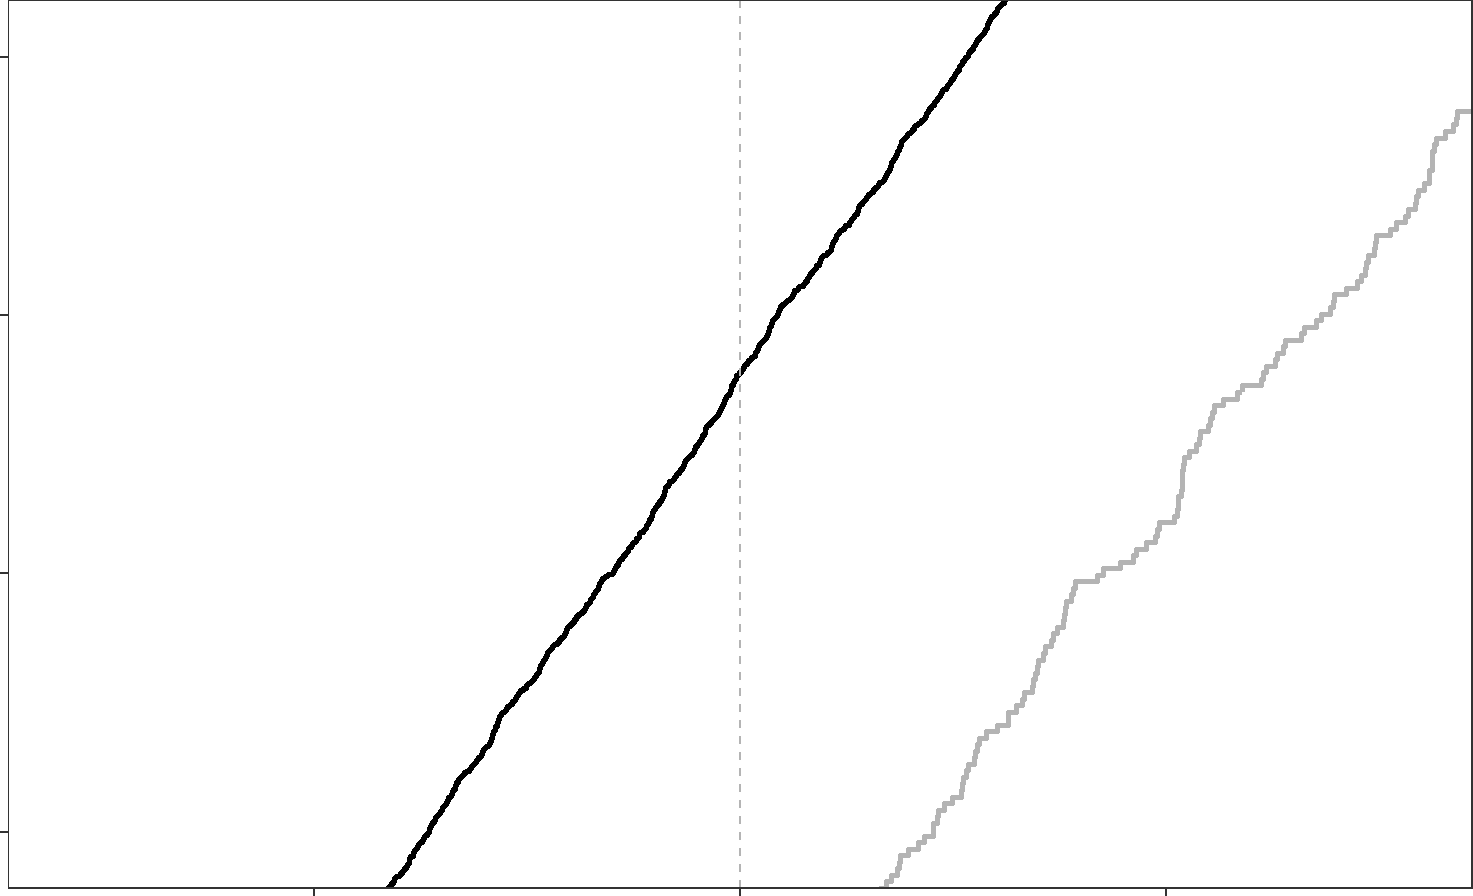
\includegraphics{Fig4_2_files/figure-latex/wobbleecdf-4.pdf}

\begin{Shaded}
\begin{Highlighting}[]
\CommentTok{\#MS}
\NormalTok{wobbleecdfMS }\OtherTok{\textless{}{-}} \FunctionTok{ggplot}\NormalTok{(MS, }\FunctionTok{aes}\NormalTok{(}\FunctionTok{as.numeric}\NormalTok{(log2FoldChange), }\AttributeTok{colour=}\FunctionTok{factor}\NormalTok{(wobble, }\AttributeTok{levels =} \FunctionTok{c}\NormalTok{(}\StringTok{"Non{-}target"}\NormalTok{, }\StringTok{"No seed"}\NormalTok{, }\StringTok{"Canonical"}\NormalTok{, }\StringTok{"Non{-}Canonical"}\NormalTok{, }\StringTok{"Multiple"}\NormalTok{)))) }\SpecialCharTok{+} 
  \FunctionTok{stat\_ecdf}\NormalTok{(}\AttributeTok{geom=}\StringTok{"step"}\NormalTok{, }\AttributeTok{linewidth=}\DecValTok{2}\NormalTok{) }\SpecialCharTok{+}
  \FunctionTok{geom\_vline}\NormalTok{(}\AttributeTok{xintercept =} \DecValTok{0}\NormalTok{, }\AttributeTok{linewidth=}\DecValTok{1}\NormalTok{, }\AttributeTok{linetype=}\StringTok{"dashed"}\NormalTok{, }\AttributeTok{colour=}\NormalTok{farbeneg) }\SpecialCharTok{+}
  \FunctionTok{scale\_colour\_manual}\NormalTok{(}\AttributeTok{values =} \FunctionTok{c}\NormalTok{(}\StringTok{"black"}\NormalTok{, farbeneg, farbe1, farbe2, farbe3)) }\SpecialCharTok{+}
  \FunctionTok{coord\_cartesian}\NormalTok{(}\AttributeTok{xlim =} \FunctionTok{c}\NormalTok{(}\SpecialCharTok{{-}}\NormalTok{xlim, xlim)) }\SpecialCharTok{+} 
  \FunctionTok{theme\_paper}\NormalTok{() }\SpecialCharTok{+}
  \FunctionTok{scale\_y\_continuous}\NormalTok{(}\StringTok{"Cumulative density"}\NormalTok{) }\SpecialCharTok{+} \FunctionTok{scale\_x\_continuous}\NormalTok{(}\StringTok{"log2FoldChange KO vs WT"}\NormalTok{) }\SpecialCharTok{+}
  \FunctionTok{ggtitle}\NormalTok{(}\StringTok{"Target genes mass spectrometry"}\NormalTok{)}

\NormalTok{wobbleecdfMS}
\end{Highlighting}
\end{Shaded}

\begin{verbatim}
## Warning: Removed 712 rows containing non-finite values (`stat_ecdf()`).
\end{verbatim}

\includegraphics{Fig4_2_files/figure-latex/wobbleecdf-5.pdf}

\begin{Shaded}
\begin{Highlighting}[]
\CommentTok{\#zoom}
\NormalTok{wobbleecdfMSZ }\OtherTok{\textless{}{-}} \FunctionTok{ggplot}\NormalTok{(MS, }\FunctionTok{aes}\NormalTok{(}\FunctionTok{as.numeric}\NormalTok{(log2FoldChange), }\AttributeTok{colour=}\FunctionTok{factor}\NormalTok{(wobble, }\AttributeTok{levels =} \FunctionTok{c}\NormalTok{(}\StringTok{"Non{-}target"}\NormalTok{, }\StringTok{"No seed"}\NormalTok{, }\StringTok{"Canonical"}\NormalTok{, }\StringTok{"Non{-}Canonical"}\NormalTok{, }\StringTok{"Multiple"}\NormalTok{)))) }\SpecialCharTok{+} 
  \FunctionTok{stat\_ecdf}\NormalTok{(}\AttributeTok{geom=}\StringTok{"step"}\NormalTok{, }\AttributeTok{linewidth=}\DecValTok{2}\SpecialCharTok{*}\NormalTok{zoomfac) }\SpecialCharTok{+}
  \FunctionTok{geom\_vline}\NormalTok{(}\AttributeTok{xintercept =} \DecValTok{0}\NormalTok{, }\AttributeTok{linewidth=}\DecValTok{1}\SpecialCharTok{*}\NormalTok{zoomfac, }\AttributeTok{linetype=}\StringTok{"dashed"}\NormalTok{, }\AttributeTok{colour=}\NormalTok{farbeneg) }\SpecialCharTok{+}
  \FunctionTok{scale\_colour\_manual}\NormalTok{(}\AttributeTok{values =} \FunctionTok{c}\NormalTok{(}\StringTok{"black"}\NormalTok{, farbeneg, farbe1, farbe2, farbe3)) }\SpecialCharTok{+}
  \FunctionTok{coord\_cartesian}\NormalTok{(}\AttributeTok{xlim =} \FunctionTok{c}\NormalTok{(}\SpecialCharTok{{-}}\NormalTok{(xlim}\SpecialCharTok{/}\DecValTok{8}\NormalTok{), (xlim}\SpecialCharTok{/}\DecValTok{8}\NormalTok{)), }\AttributeTok{ylim =} \FunctionTok{c}\NormalTok{(}\FloatTok{0.5}\DecValTok{{-}1}\SpecialCharTok{/}\DecValTok{16}\NormalTok{, }\FloatTok{0.5}\SpecialCharTok{+}\DecValTok{1}\SpecialCharTok{/}\DecValTok{16}\NormalTok{)) }\SpecialCharTok{+} 
  \FunctionTok{theme\_bw}\NormalTok{() }\SpecialCharTok{+}
  \FunctionTok{theme}\NormalTok{(}\AttributeTok{legend.position =} \StringTok{"none"}\NormalTok{, }\AttributeTok{axis.text =} \FunctionTok{element\_blank}\NormalTok{(), }\AttributeTok{panel.grid =} \FunctionTok{element\_blank}\NormalTok{(),}
        \AttributeTok{panel.background =} \FunctionTok{element\_rect}\NormalTok{(}\AttributeTok{fill=}\StringTok{\textquotesingle{}transparent\textquotesingle{}}\NormalTok{), }\CommentTok{\#transparent panel bg}
        \AttributeTok{plot.background =} \FunctionTok{element\_rect}\NormalTok{(}\AttributeTok{fill=}\StringTok{\textquotesingle{}transparent\textquotesingle{}}\NormalTok{, }\AttributeTok{color=}\ConstantTok{NA}\NormalTok{)) }\SpecialCharTok{+}
  \FunctionTok{scale\_y\_continuous}\NormalTok{(}\StringTok{""}\NormalTok{) }\SpecialCharTok{+} \FunctionTok{scale\_x\_continuous}\NormalTok{(}\StringTok{""}\NormalTok{)}


\NormalTok{wobbleecdfMSZ}
\end{Highlighting}
\end{Shaded}

\begin{verbatim}
## Warning: Removed 712 rows containing non-finite values (`stat_ecdf()`).
\end{verbatim}

\includegraphics{Fig4_2_files/figure-latex/wobbleecdf-6.pdf}

\begin{Shaded}
\begin{Highlighting}[]
\CommentTok{\#TE}
\NormalTok{wobbleecdfTE }\OtherTok{\textless{}{-}} \FunctionTok{ggplot}\NormalTok{(TE, }\FunctionTok{aes}\NormalTok{(}\FunctionTok{as.numeric}\NormalTok{(log2FoldChange), }\AttributeTok{colour=}\FunctionTok{factor}\NormalTok{(wobble, }\AttributeTok{levels =} \FunctionTok{c}\NormalTok{(}\StringTok{"Non{-}target"}\NormalTok{, }\StringTok{"No seed"}\NormalTok{, }\StringTok{"Canonical"}\NormalTok{, }\StringTok{"Non{-}Canonical"}\NormalTok{, }\StringTok{"Multiple"}\NormalTok{)))) }\SpecialCharTok{+} 
  \FunctionTok{stat\_ecdf}\NormalTok{(}\AttributeTok{geom=}\StringTok{"step"}\NormalTok{, }\AttributeTok{linewidth=}\DecValTok{2}\NormalTok{) }\SpecialCharTok{+}
  \FunctionTok{geom\_vline}\NormalTok{(}\AttributeTok{xintercept =} \DecValTok{0}\NormalTok{, }\AttributeTok{linewidth=}\DecValTok{1}\NormalTok{, }\AttributeTok{linetype=}\StringTok{"dashed"}\NormalTok{, }\AttributeTok{colour=}\NormalTok{farbeneg) }\SpecialCharTok{+}
  \FunctionTok{scale\_colour\_manual}\NormalTok{(}\AttributeTok{values =} \FunctionTok{c}\NormalTok{(}\StringTok{"black"}\NormalTok{, farbeneg, farbe1, farbe2, farbe3)) }\SpecialCharTok{+}
  \FunctionTok{coord\_cartesian}\NormalTok{(}\AttributeTok{xlim =} \FunctionTok{c}\NormalTok{(}\SpecialCharTok{{-}}\NormalTok{xlim, xlim)) }\SpecialCharTok{+} 
  \FunctionTok{theme\_paper}\NormalTok{() }\SpecialCharTok{+}
  \FunctionTok{scale\_y\_continuous}\NormalTok{(}\StringTok{"Cumulative density"}\NormalTok{) }\SpecialCharTok{+} \FunctionTok{scale\_x\_continuous}\NormalTok{(}\StringTok{"log2FoldChange KO vs WT"}\NormalTok{) }\SpecialCharTok{+}
  \FunctionTok{ggtitle}\NormalTok{(}\StringTok{"Target genes translational efficiency"}\NormalTok{)}

\NormalTok{wobbleecdfTE}
\end{Highlighting}
\end{Shaded}

\includegraphics{Fig4_2_files/figure-latex/wobbleecdf-7.pdf}

\begin{Shaded}
\begin{Highlighting}[]
\CommentTok{\#zoom}
\NormalTok{wobbleecdfTEZ }\OtherTok{\textless{}{-}} \FunctionTok{ggplot}\NormalTok{(TE, }\FunctionTok{aes}\NormalTok{(}\FunctionTok{as.numeric}\NormalTok{(log2FoldChange), }\AttributeTok{colour=}\FunctionTok{factor}\NormalTok{(wobble, }\AttributeTok{levels =} \FunctionTok{c}\NormalTok{(}\StringTok{"Non{-}target"}\NormalTok{, }\StringTok{"No seed"}\NormalTok{, }\StringTok{"Canonical"}\NormalTok{, }\StringTok{"Non{-}Canonical"}\NormalTok{, }\StringTok{"Multiple"}\NormalTok{)))) }\SpecialCharTok{+} 
  \FunctionTok{stat\_ecdf}\NormalTok{(}\AttributeTok{geom=}\StringTok{"step"}\NormalTok{, }\AttributeTok{linewidth=}\DecValTok{2}\SpecialCharTok{*}\NormalTok{zoomfac) }\SpecialCharTok{+}
  \FunctionTok{geom\_vline}\NormalTok{(}\AttributeTok{xintercept =} \DecValTok{0}\NormalTok{, }\AttributeTok{linewidth=}\DecValTok{1}\SpecialCharTok{*}\NormalTok{zoomfac, }\AttributeTok{linetype=}\StringTok{"dashed"}\NormalTok{, }\AttributeTok{colour=}\NormalTok{farbeneg) }\SpecialCharTok{+}
  \FunctionTok{scale\_colour\_manual}\NormalTok{(}\AttributeTok{values =} \FunctionTok{c}\NormalTok{(}\StringTok{"black"}\NormalTok{, farbeneg, farbe1, farbe2, farbe3)) }\SpecialCharTok{+}
  \FunctionTok{coord\_cartesian}\NormalTok{(}\AttributeTok{xlim =} \FunctionTok{c}\NormalTok{(}\SpecialCharTok{{-}}\NormalTok{(xlim}\SpecialCharTok{/}\DecValTok{8}\NormalTok{), (xlim}\SpecialCharTok{/}\DecValTok{8}\NormalTok{)), }\AttributeTok{ylim =} \FunctionTok{c}\NormalTok{(}\FloatTok{0.5}\DecValTok{{-}1}\SpecialCharTok{/}\DecValTok{16}\NormalTok{, }\FloatTok{0.5}\SpecialCharTok{+}\DecValTok{1}\SpecialCharTok{/}\DecValTok{16}\NormalTok{)) }\SpecialCharTok{+} 
  \FunctionTok{theme\_bw}\NormalTok{() }\SpecialCharTok{+}
  \FunctionTok{theme}\NormalTok{(}\AttributeTok{legend.position =} \StringTok{"none"}\NormalTok{, }\AttributeTok{axis.text =} \FunctionTok{element\_blank}\NormalTok{(), }\AttributeTok{panel.grid =} \FunctionTok{element\_blank}\NormalTok{(),}
        \AttributeTok{panel.background =} \FunctionTok{element\_rect}\NormalTok{(}\AttributeTok{fill=}\StringTok{\textquotesingle{}transparent\textquotesingle{}}\NormalTok{), }\CommentTok{\#transparent panel bg}
        \AttributeTok{plot.background =} \FunctionTok{element\_rect}\NormalTok{(}\AttributeTok{fill=}\StringTok{\textquotesingle{}transparent\textquotesingle{}}\NormalTok{, }\AttributeTok{color=}\ConstantTok{NA}\NormalTok{)) }\SpecialCharTok{+}
  \FunctionTok{scale\_y\_continuous}\NormalTok{(}\StringTok{""}\NormalTok{) }\SpecialCharTok{+} \FunctionTok{scale\_x\_continuous}\NormalTok{(}\StringTok{""}\NormalTok{)}


\NormalTok{wobbleecdfTEZ}
\end{Highlighting}
\end{Shaded}

\includegraphics{Fig4_2_files/figure-latex/wobbleecdf-8.pdf}

\begin{Shaded}
\begin{Highlighting}[]
\CommentTok{\#export RNA}
\FunctionTok{pdf}\NormalTok{(}\StringTok{"C:/Users/nikit/Documents/Krueger\_Lab/Publications/miR181\_paper/Figure4/wobbleECDF\_RNA.pdf"}\NormalTok{, }\AttributeTok{width=}\DecValTok{2}\NormalTok{, }\AttributeTok{height =} \DecValTok{2}\NormalTok{)}
\NormalTok{wobbleecdfRNA}
\FunctionTok{dev.off}\NormalTok{()}
\end{Highlighting}
\end{Shaded}

\begin{verbatim}
## pdf 
##   2
\end{verbatim}

\begin{Shaded}
\begin{Highlighting}[]
\FunctionTok{pdf}\NormalTok{(}\StringTok{"C:/Users/nikit/Documents/Krueger\_Lab/Publications/miR181\_paper/Figure4/wobbleECDF\_RNA\_zoom.pdf"}\NormalTok{, }\AttributeTok{width=}\DecValTok{2}\SpecialCharTok{*}\NormalTok{zoomfac, }\AttributeTok{height =} \DecValTok{2}\SpecialCharTok{*}\NormalTok{zoomfac)}
\NormalTok{wobbleecdfRNAZ}
\FunctionTok{dev.off}\NormalTok{()}
\end{Highlighting}
\end{Shaded}

\begin{verbatim}
## pdf 
##   2
\end{verbatim}

\begin{Shaded}
\begin{Highlighting}[]
\CommentTok{\#export RPF}
\FunctionTok{pdf}\NormalTok{(}\StringTok{"C:/Users/nikit/Documents/Krueger\_Lab/Publications/miR181\_paper/Figure4/wobbleECDF\_RPF.pdf"}\NormalTok{, }\AttributeTok{width=}\DecValTok{2}\NormalTok{, }\AttributeTok{height =} \DecValTok{2}\NormalTok{)}
\NormalTok{wobbleecdfRPF}
\FunctionTok{dev.off}\NormalTok{()}
\end{Highlighting}
\end{Shaded}

\begin{verbatim}
## pdf 
##   2
\end{verbatim}

\begin{Shaded}
\begin{Highlighting}[]
\FunctionTok{pdf}\NormalTok{(}\StringTok{"C:/Users/nikit/Documents/Krueger\_Lab/Publications/miR181\_paper/Figure4/wobbleECDF\_RPF\_zoom.pdf"}\NormalTok{, }\AttributeTok{width=}\DecValTok{2}\SpecialCharTok{*}\NormalTok{zoomfac, }\AttributeTok{height =} \DecValTok{2}\SpecialCharTok{*}\NormalTok{zoomfac)}
\NormalTok{wobbleecdfRPFZ}
\FunctionTok{dev.off}\NormalTok{()}
\end{Highlighting}
\end{Shaded}

\begin{verbatim}
## pdf 
##   2
\end{verbatim}

\begin{Shaded}
\begin{Highlighting}[]
\CommentTok{\#export MS}
\FunctionTok{pdf}\NormalTok{(}\StringTok{"C:/Users/nikit/Documents/Krueger\_Lab/Publications/miR181\_paper/Figure4/wobbleECDF\_MS.pdf"}\NormalTok{, }\AttributeTok{width=}\DecValTok{2}\NormalTok{, }\AttributeTok{height =} \DecValTok{2}\NormalTok{)}
\NormalTok{wobbleecdfMS}
\end{Highlighting}
\end{Shaded}

\begin{verbatim}
## Warning: Removed 712 rows containing non-finite values (`stat_ecdf()`).
\end{verbatim}

\begin{Shaded}
\begin{Highlighting}[]
\FunctionTok{dev.off}\NormalTok{()}
\end{Highlighting}
\end{Shaded}

\begin{verbatim}
## pdf 
##   2
\end{verbatim}

\begin{Shaded}
\begin{Highlighting}[]
\FunctionTok{pdf}\NormalTok{(}\StringTok{"C:/Users/nikit/Documents/Krueger\_Lab/Publications/miR181\_paper/Figure4/wobbleECDF\_MS\_zoom.pdf"}\NormalTok{, }\AttributeTok{width=}\DecValTok{2}\SpecialCharTok{*}\NormalTok{zoomfac, }\AttributeTok{height =} \DecValTok{2}\SpecialCharTok{*}\NormalTok{zoomfac)}
\NormalTok{wobbleecdfMSZ}
\end{Highlighting}
\end{Shaded}

\begin{verbatim}
## Warning: Removed 712 rows containing non-finite values (`stat_ecdf()`).
\end{verbatim}

\begin{Shaded}
\begin{Highlighting}[]
\FunctionTok{dev.off}\NormalTok{()}
\end{Highlighting}
\end{Shaded}

\begin{verbatim}
## pdf 
##   2
\end{verbatim}

\begin{Shaded}
\begin{Highlighting}[]
\CommentTok{\#export TE}
\FunctionTok{pdf}\NormalTok{(}\StringTok{"C:/Users/nikit/Documents/Krueger\_Lab/Publications/miR181\_paper/Figure4/wobbleECDF\_TE.pdf"}\NormalTok{, }\AttributeTok{width=}\DecValTok{2}\NormalTok{, }\AttributeTok{height =} \DecValTok{2}\NormalTok{)}
\NormalTok{wobbleecdfTE}
\FunctionTok{dev.off}\NormalTok{()}
\end{Highlighting}
\end{Shaded}

\begin{verbatim}
## pdf 
##   2
\end{verbatim}

\begin{Shaded}
\begin{Highlighting}[]
\FunctionTok{pdf}\NormalTok{(}\StringTok{"C:/Users/nikit/Documents/Krueger\_Lab/Publications/miR181\_paper/Figure4/wobbleECDF\_TE\_zoom.pdf"}\NormalTok{, }\AttributeTok{width=}\DecValTok{2}\SpecialCharTok{*}\NormalTok{zoomfac, }\AttributeTok{height =} \DecValTok{2}\SpecialCharTok{*}\NormalTok{zoomfac)}
\NormalTok{wobbleecdfTEZ}
\FunctionTok{dev.off}\NormalTok{()}
\end{Highlighting}
\end{Shaded}

\begin{verbatim}
## pdf 
##   2
\end{verbatim}

\begin{Shaded}
\begin{Highlighting}[]
\FunctionTok{table}\NormalTok{(RPF}\SpecialCharTok{$}\NormalTok{wobble)}
\end{Highlighting}
\end{Shaded}

\begin{verbatim}
## 
##     Canonical      Multiple       No seed Non-Canonical    Non-target 
##           295           990           713           149          9222
\end{verbatim}

\hypertarget{te-density-wobble}{%
\section{TE density wobble}\label{te-density-wobble}}

\begin{Shaded}
\begin{Highlighting}[]
\NormalTok{TEdenswob }\OtherTok{\textless{}{-}} \FunctionTok{ggplot}\NormalTok{(TE, }\FunctionTok{aes}\NormalTok{(}\AttributeTok{x=}\NormalTok{log2FoldChange, }\AttributeTok{colour=}\FunctionTok{factor}\NormalTok{(wobble, }\AttributeTok{levels =} \FunctionTok{c}\NormalTok{(}\StringTok{"No seed"}\NormalTok{, }\StringTok{"Canonical"}\NormalTok{, }\StringTok{"Non{-}Canonical"}\NormalTok{, }\StringTok{"Multiple"}\NormalTok{, }\StringTok{"Non{-}target"}\NormalTok{)))) }\SpecialCharTok{+}
  \FunctionTok{geom\_density}\NormalTok{() }\SpecialCharTok{+}
  \FunctionTok{geom\_vline}\NormalTok{(}\AttributeTok{xintercept =} \DecValTok{0}\NormalTok{, }\AttributeTok{linewidth=}\DecValTok{1}\NormalTok{, }\AttributeTok{linetype=}\StringTok{"dashed"}\NormalTok{, }\AttributeTok{colour=}\NormalTok{farbeneg) }\SpecialCharTok{+}
  \FunctionTok{scale\_colour\_manual}\NormalTok{(}\AttributeTok{values =} \FunctionTok{c}\NormalTok{( farbeneg, farbe1, farbe2, farbe3, }\StringTok{"black"}\NormalTok{)) }\SpecialCharTok{+}
  \FunctionTok{theme\_paper}\NormalTok{() }\SpecialCharTok{+}
  \FunctionTok{coord\_cartesian}\NormalTok{(}\AttributeTok{xlim =} \FunctionTok{c}\NormalTok{(}\SpecialCharTok{{-}}\DecValTok{1}\NormalTok{,}\DecValTok{1}\NormalTok{)) }\SpecialCharTok{+}
  \FunctionTok{ggtitle}\NormalTok{(}\StringTok{"TE"}\NormalTok{)}

\NormalTok{TEdenswob}
\end{Highlighting}
\end{Shaded}

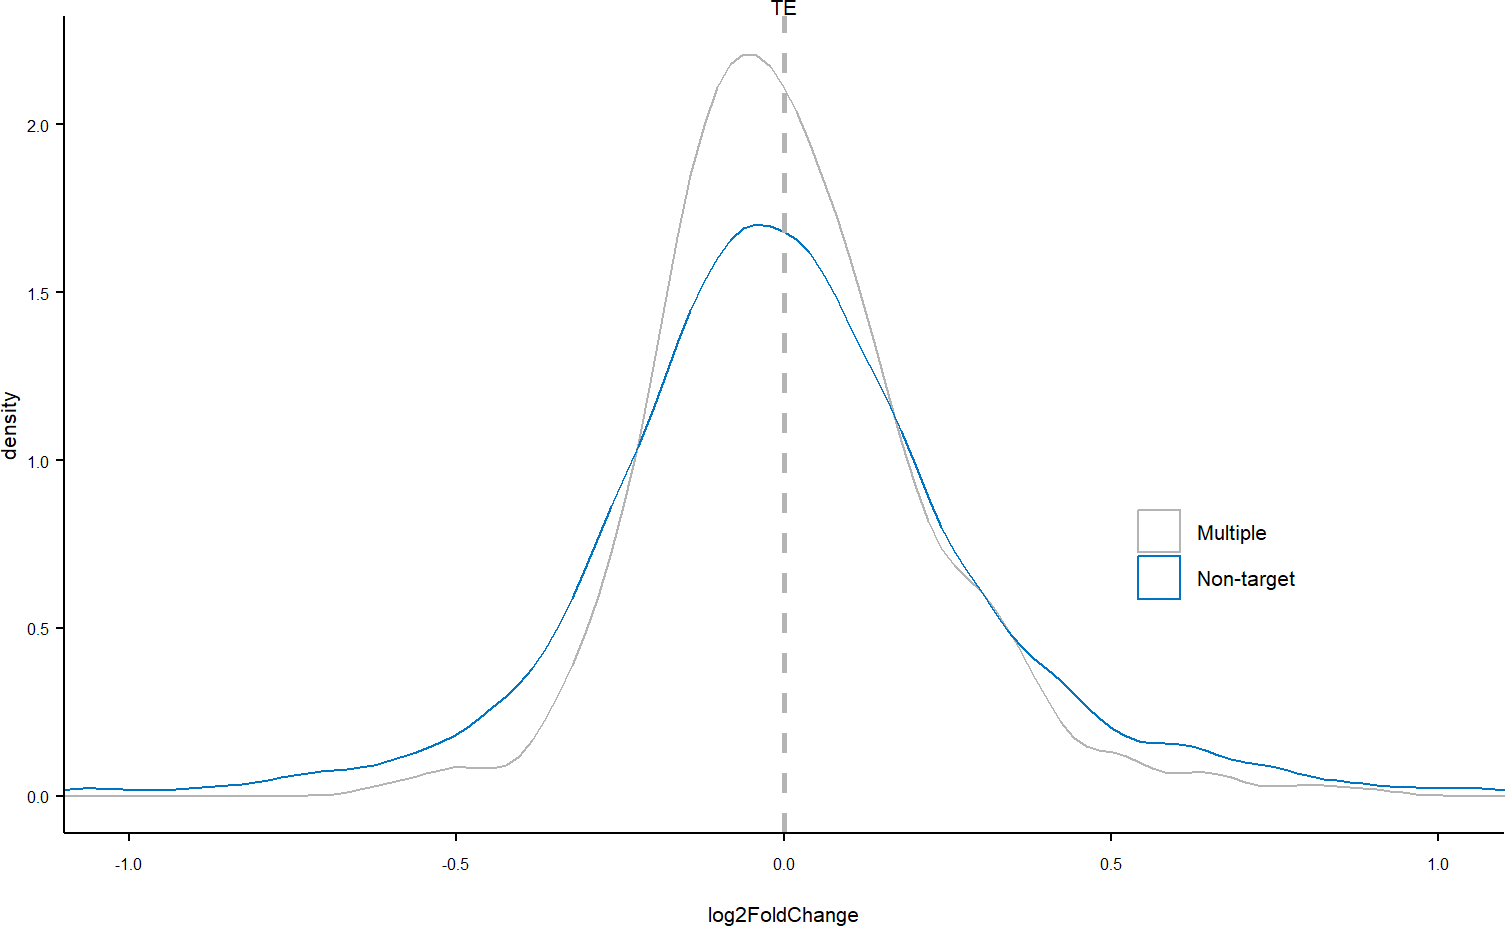
\includegraphics{Fig4_2_files/figure-latex/TEdensitywobble-1.pdf}

\begin{Shaded}
\begin{Highlighting}[]
\FunctionTok{pdf}\NormalTok{(}\StringTok{"C:/Users/nikit/Documents/Krueger\_Lab/Publications/miR181\_paper/Figure4/WobbleDensity\_TE.pdf"}\NormalTok{, }\AttributeTok{width=}\DecValTok{2}\NormalTok{, }\AttributeTok{height =} \DecValTok{2}\NormalTok{)}
\NormalTok{TEdenswob}
\FunctionTok{dev.off}\NormalTok{()}
\end{Highlighting}
\end{Shaded}

\begin{verbatim}
## pdf 
##   2
\end{verbatim}

\hypertarget{significance}{%
\subsection{Significance}\label{significance}}

\begin{Shaded}
\begin{Highlighting}[]
\NormalTok{RNAWobbleTTest1 }\OtherTok{\textless{}{-}} \FunctionTok{t.test}\NormalTok{(RNA[RNA}\SpecialCharTok{$}\NormalTok{wobble}\SpecialCharTok{==}\StringTok{"No seed"}\NormalTok{, }\StringTok{"log2FoldChange"}\NormalTok{], RNA[RNA}\SpecialCharTok{$}\NormalTok{wobble}\SpecialCharTok{==}\StringTok{"Non{-}target"}\NormalTok{, }\StringTok{"log2FoldChange"}\NormalTok{])}
\NormalTok{RNAWobbleTTest2 }\OtherTok{\textless{}{-}} \FunctionTok{t.test}\NormalTok{(RNA[RNA}\SpecialCharTok{$}\NormalTok{wobble}\SpecialCharTok{==}\StringTok{"Canonical"}\NormalTok{, }\StringTok{"log2FoldChange"}\NormalTok{], RNA[RNA}\SpecialCharTok{$}\NormalTok{wobble}\SpecialCharTok{==}\StringTok{"Non{-}target"}\NormalTok{, }\StringTok{"log2FoldChange"}\NormalTok{])}
\NormalTok{RNAWobbleTTest3 }\OtherTok{\textless{}{-}} \FunctionTok{t.test}\NormalTok{(RNA[RNA}\SpecialCharTok{$}\NormalTok{wobble}\SpecialCharTok{==}\StringTok{"Non{-}Canonical"}\NormalTok{, }\StringTok{"log2FoldChange"}\NormalTok{], RNA[RNA}\SpecialCharTok{$}\NormalTok{wobble}\SpecialCharTok{==}\StringTok{"Non{-}target"}\NormalTok{, }\StringTok{"log2FoldChange"}\NormalTok{])}

\NormalTok{RPFWobbleTTest1 }\OtherTok{\textless{}{-}} \FunctionTok{t.test}\NormalTok{(RPF[RPF}\SpecialCharTok{$}\NormalTok{wobble}\SpecialCharTok{==}\StringTok{"No seed"}\NormalTok{, }\StringTok{"log2FoldChange"}\NormalTok{], RPF[RPF}\SpecialCharTok{$}\NormalTok{wobble}\SpecialCharTok{==}\StringTok{"Non{-}target"}\NormalTok{, }\StringTok{"log2FoldChange"}\NormalTok{])}
\NormalTok{RPFWobbleTTest2 }\OtherTok{\textless{}{-}} \FunctionTok{t.test}\NormalTok{(RPF[RPF}\SpecialCharTok{$}\NormalTok{wobble}\SpecialCharTok{==}\StringTok{"Canonical"}\NormalTok{, }\StringTok{"log2FoldChange"}\NormalTok{], RPF[RPF}\SpecialCharTok{$}\NormalTok{wobble}\SpecialCharTok{==}\StringTok{"Non{-}target"}\NormalTok{, }\StringTok{"log2FoldChange"}\NormalTok{])}
\NormalTok{RPFWobbleTTest3 }\OtherTok{\textless{}{-}} \FunctionTok{t.test}\NormalTok{(RPF[RPF}\SpecialCharTok{$}\NormalTok{wobble}\SpecialCharTok{==}\StringTok{"Non{-}Canonical"}\NormalTok{, }\StringTok{"log2FoldChange"}\NormalTok{], RPF[RPF}\SpecialCharTok{$}\NormalTok{wobble}\SpecialCharTok{==}\StringTok{"Non{-}target"}\NormalTok{, }\StringTok{"log2FoldChange"}\NormalTok{])}

\NormalTok{TEWobbleTTest1 }\OtherTok{\textless{}{-}} \FunctionTok{t.test}\NormalTok{(TE[TE}\SpecialCharTok{$}\NormalTok{wobble}\SpecialCharTok{==}\StringTok{"No seed"}\NormalTok{, }\StringTok{"log2FoldChange"}\NormalTok{], TE[TE}\SpecialCharTok{$}\NormalTok{wobble}\SpecialCharTok{==}\StringTok{"Non{-}target"}\NormalTok{, }\StringTok{"log2FoldChange"}\NormalTok{])}
\NormalTok{TEWobbleTTest2 }\OtherTok{\textless{}{-}} \FunctionTok{t.test}\NormalTok{(TE[TE}\SpecialCharTok{$}\NormalTok{wobble}\SpecialCharTok{==}\StringTok{"Canonical"}\NormalTok{, }\StringTok{"log2FoldChange"}\NormalTok{], TE[TE}\SpecialCharTok{$}\NormalTok{wobble}\SpecialCharTok{==}\StringTok{"Non{-}target"}\NormalTok{, }\StringTok{"log2FoldChange"}\NormalTok{])}
\NormalTok{TEWobbleTTest3 }\OtherTok{\textless{}{-}} \FunctionTok{t.test}\NormalTok{(TE[TE}\SpecialCharTok{$}\NormalTok{wobble}\SpecialCharTok{==}\StringTok{"Non{-}Canonical"}\NormalTok{, }\StringTok{"log2FoldChange"}\NormalTok{], TE[TE}\SpecialCharTok{$}\NormalTok{wobble}\SpecialCharTok{==}\StringTok{"Non{-}target"}\NormalTok{, }\StringTok{"log2FoldChange"}\NormalTok{])}

\NormalTok{MSWobbleTTest1 }\OtherTok{\textless{}{-}} \FunctionTok{t.test}\NormalTok{(MS[MS}\SpecialCharTok{$}\NormalTok{wobble}\SpecialCharTok{==}\StringTok{"No seed"}\NormalTok{, }\StringTok{"log2FoldChange"}\NormalTok{], MS[MS}\SpecialCharTok{$}\NormalTok{wobble}\SpecialCharTok{==}\StringTok{"Non{-}target"}\NormalTok{, }\StringTok{"log2FoldChange"}\NormalTok{])}
\NormalTok{MSWobbleTTest2 }\OtherTok{\textless{}{-}} \FunctionTok{t.test}\NormalTok{(MS[MS}\SpecialCharTok{$}\NormalTok{wobble}\SpecialCharTok{==}\StringTok{"Canonical"}\NormalTok{, }\StringTok{"log2FoldChange"}\NormalTok{], MS[MS}\SpecialCharTok{$}\NormalTok{wobble}\SpecialCharTok{==}\StringTok{"Non{-}target"}\NormalTok{, }\StringTok{"log2FoldChange"}\NormalTok{])}
\NormalTok{MSWobbleTTest3 }\OtherTok{\textless{}{-}} \FunctionTok{t.test}\NormalTok{(MS[MS}\SpecialCharTok{$}\NormalTok{wobble}\SpecialCharTok{==}\StringTok{"Non{-}Canonical"}\NormalTok{, }\StringTok{"log2FoldChange"}\NormalTok{], MS[MS}\SpecialCharTok{$}\NormalTok{wobble}\SpecialCharTok{==}\StringTok{"Non{-}target"}\NormalTok{, }\StringTok{"log2FoldChange"}\NormalTok{])}

\CommentTok{\#kolmogorov{-}smirnov}
\NormalTok{RNAWobbleksTest1 }\OtherTok{\textless{}{-}} \FunctionTok{ks.test}\NormalTok{(RNA[RNA}\SpecialCharTok{$}\NormalTok{wobble}\SpecialCharTok{==}\StringTok{"No seed"}\NormalTok{, }\StringTok{"log2FoldChange"}\NormalTok{], RNA[RNA}\SpecialCharTok{$}\NormalTok{wobble}\SpecialCharTok{==}\StringTok{"Non{-}target"}\NormalTok{, }\StringTok{"log2FoldChange"}\NormalTok{])}
\end{Highlighting}
\end{Shaded}

\begin{verbatim}
## Warning in ks.test.default(RNA[RNA$wobble == "No seed", "log2FoldChange"], :
## p-value will be approximate in the presence of ties
\end{verbatim}

\begin{Shaded}
\begin{Highlighting}[]
\NormalTok{RNAWobbleksTest2 }\OtherTok{\textless{}{-}} \FunctionTok{ks.test}\NormalTok{(RNA[RNA}\SpecialCharTok{$}\NormalTok{wobble}\SpecialCharTok{==}\StringTok{"Canonical"}\NormalTok{, }\StringTok{"log2FoldChange"}\NormalTok{], RNA[RNA}\SpecialCharTok{$}\NormalTok{wobble}\SpecialCharTok{==}\StringTok{"Non{-}target"}\NormalTok{, }\StringTok{"log2FoldChange"}\NormalTok{])}
\end{Highlighting}
\end{Shaded}

\begin{verbatim}
## Warning in ks.test.default(RNA[RNA$wobble == "Canonical", "log2FoldChange"], :
## p-value will be approximate in the presence of ties
\end{verbatim}

\begin{Shaded}
\begin{Highlighting}[]
\NormalTok{RNAWobbleksTest3 }\OtherTok{\textless{}{-}} \FunctionTok{ks.test}\NormalTok{(RNA[RNA}\SpecialCharTok{$}\NormalTok{wobble}\SpecialCharTok{==}\StringTok{"Non{-}Canonical"}\NormalTok{, }\StringTok{"log2FoldChange"}\NormalTok{], RNA[RNA}\SpecialCharTok{$}\NormalTok{wobble}\SpecialCharTok{==}\StringTok{"Non{-}target"}\NormalTok{, }\StringTok{"log2FoldChange"}\NormalTok{])}
\end{Highlighting}
\end{Shaded}

\begin{verbatim}
## Warning in ks.test.default(RNA[RNA$wobble == "Non-Canonical",
## "log2FoldChange"], : p-value will be approximate in the presence of ties
\end{verbatim}

\begin{Shaded}
\begin{Highlighting}[]
\NormalTok{RPFWobbleksTest1 }\OtherTok{\textless{}{-}} \FunctionTok{ks.test}\NormalTok{(RPF[RPF}\SpecialCharTok{$}\NormalTok{wobble}\SpecialCharTok{==}\StringTok{"No seed"}\NormalTok{, }\StringTok{"log2FoldChange"}\NormalTok{], RPF[RPF}\SpecialCharTok{$}\NormalTok{wobble}\SpecialCharTok{==}\StringTok{"Non{-}target"}\NormalTok{, }\StringTok{"log2FoldChange"}\NormalTok{])}
\end{Highlighting}
\end{Shaded}

\begin{verbatim}
## Warning in ks.test.default(RPF[RPF$wobble == "No seed", "log2FoldChange"], :
## p-value will be approximate in the presence of ties
\end{verbatim}

\begin{Shaded}
\begin{Highlighting}[]
\NormalTok{RPFWobbleksTest2 }\OtherTok{\textless{}{-}} \FunctionTok{ks.test}\NormalTok{(RPF[RPF}\SpecialCharTok{$}\NormalTok{wobble}\SpecialCharTok{==}\StringTok{"Canonical"}\NormalTok{, }\StringTok{"log2FoldChange"}\NormalTok{], RPF[RPF}\SpecialCharTok{$}\NormalTok{wobble}\SpecialCharTok{==}\StringTok{"Non{-}target"}\NormalTok{, }\StringTok{"log2FoldChange"}\NormalTok{])}
\end{Highlighting}
\end{Shaded}

\begin{verbatim}
## Warning in ks.test.default(RPF[RPF$wobble == "Canonical", "log2FoldChange"], :
## p-value will be approximate in the presence of ties
\end{verbatim}

\begin{Shaded}
\begin{Highlighting}[]
\NormalTok{RPFWobbleksTest3 }\OtherTok{\textless{}{-}} \FunctionTok{ks.test}\NormalTok{(RPF[RPF}\SpecialCharTok{$}\NormalTok{wobble}\SpecialCharTok{==}\StringTok{"Non{-}Canonical"}\NormalTok{, }\StringTok{"log2FoldChange"}\NormalTok{], RPF[RPF}\SpecialCharTok{$}\NormalTok{wobble}\SpecialCharTok{==}\StringTok{"Non{-}target"}\NormalTok{, }\StringTok{"log2FoldChange"}\NormalTok{])}
\end{Highlighting}
\end{Shaded}

\begin{verbatim}
## Warning in ks.test.default(RPF[RPF$wobble == "Non-Canonical",
## "log2FoldChange"], : p-value will be approximate in the presence of ties
\end{verbatim}

\begin{Shaded}
\begin{Highlighting}[]
\NormalTok{TEWobbleksTest1 }\OtherTok{\textless{}{-}} \FunctionTok{ks.test}\NormalTok{(TE[TE}\SpecialCharTok{$}\NormalTok{wobble}\SpecialCharTok{==}\StringTok{"No seed"}\NormalTok{, }\StringTok{"log2FoldChange"}\NormalTok{], TE[TE}\SpecialCharTok{$}\NormalTok{wobble}\SpecialCharTok{==}\StringTok{"Non{-}target"}\NormalTok{, }\StringTok{"log2FoldChange"}\NormalTok{])}
\NormalTok{TEWobbleksTest2 }\OtherTok{\textless{}{-}} \FunctionTok{ks.test}\NormalTok{(TE[TE}\SpecialCharTok{$}\NormalTok{wobble}\SpecialCharTok{==}\StringTok{"Canonical"}\NormalTok{, }\StringTok{"log2FoldChange"}\NormalTok{], TE[TE}\SpecialCharTok{$}\NormalTok{wobble}\SpecialCharTok{==}\StringTok{"Non{-}target"}\NormalTok{, }\StringTok{"log2FoldChange"}\NormalTok{])}
\NormalTok{TEWobbleksTest3 }\OtherTok{\textless{}{-}} \FunctionTok{ks.test}\NormalTok{(TE[TE}\SpecialCharTok{$}\NormalTok{wobble}\SpecialCharTok{==}\StringTok{"Non{-}Canonical"}\NormalTok{, }\StringTok{"log2FoldChange"}\NormalTok{], TE[TE}\SpecialCharTok{$}\NormalTok{wobble}\SpecialCharTok{==}\StringTok{"Non{-}target"}\NormalTok{, }\StringTok{"log2FoldChange"}\NormalTok{])}

\NormalTok{MSWobbleksTest1 }\OtherTok{\textless{}{-}} \FunctionTok{ks.test}\NormalTok{(MS[MS}\SpecialCharTok{$}\NormalTok{wobble}\SpecialCharTok{==}\StringTok{"No seed"}\NormalTok{, }\StringTok{"log2FoldChange"}\NormalTok{], MS[MS}\SpecialCharTok{$}\NormalTok{wobble}\SpecialCharTok{==}\StringTok{"Non{-}target"}\NormalTok{, }\StringTok{"log2FoldChange"}\NormalTok{])}
\end{Highlighting}
\end{Shaded}

\begin{verbatim}
## Warning in ks.test.default(MS[MS$wobble == "No seed", "log2FoldChange"], :
## p-value will be approximate in the presence of ties
\end{verbatim}

\begin{Shaded}
\begin{Highlighting}[]
\NormalTok{MSWobbleksTest2 }\OtherTok{\textless{}{-}} \FunctionTok{ks.test}\NormalTok{(MS[MS}\SpecialCharTok{$}\NormalTok{wobble}\SpecialCharTok{==}\StringTok{"Canonical"}\NormalTok{, }\StringTok{"log2FoldChange"}\NormalTok{], MS[MS}\SpecialCharTok{$}\NormalTok{wobble}\SpecialCharTok{==}\StringTok{"Non{-}target"}\NormalTok{, }\StringTok{"log2FoldChange"}\NormalTok{])}
\end{Highlighting}
\end{Shaded}

\begin{verbatim}
## Warning in ks.test.default(MS[MS$wobble == "Canonical", "log2FoldChange"], :
## p-value will be approximate in the presence of ties
\end{verbatim}

\begin{Shaded}
\begin{Highlighting}[]
\NormalTok{MSWobbleksTest3 }\OtherTok{\textless{}{-}} \FunctionTok{ks.test}\NormalTok{(MS[MS}\SpecialCharTok{$}\NormalTok{wobble}\SpecialCharTok{==}\StringTok{"Non{-}Canonical"}\NormalTok{, }\StringTok{"log2FoldChange"}\NormalTok{], MS[MS}\SpecialCharTok{$}\NormalTok{wobble}\SpecialCharTok{==}\StringTok{"Non{-}target"}\NormalTok{, }\StringTok{"log2FoldChange"}\NormalTok{])}
\end{Highlighting}
\end{Shaded}

\begin{verbatim}
## Warning in ks.test.default(MS[MS$wobble == "Non-Canonical", "log2FoldChange"],
## : p-value will be approximate in the presence of ties
\end{verbatim}

\begin{Shaded}
\begin{Highlighting}[]
\NormalTok{Wobblesig }\OtherTok{\textless{}{-}} \FunctionTok{data.frame}\NormalTok{(}\FunctionTok{c}\NormalTok{(}\StringTok{"RNA"}\NormalTok{, }\StringTok{"RNA"}\NormalTok{, }\StringTok{"RNA"}\NormalTok{, }\StringTok{"RPF"}\NormalTok{, }\StringTok{"RPF"}\NormalTok{, }\StringTok{"RPF"}\NormalTok{, }\StringTok{"TE"}\NormalTok{, }\StringTok{"TE"}\NormalTok{, }\StringTok{"TE"}\NormalTok{, }\StringTok{"MS"}\NormalTok{, }\StringTok{"MS"}\NormalTok{, }\StringTok{"MS"}\NormalTok{),}
                        \FunctionTok{c}\NormalTok{(}\StringTok{"No seed"}\NormalTok{, }\StringTok{"Canonical"}\NormalTok{, }\StringTok{"Non{-}Canonical"}\NormalTok{, }\StringTok{"No seed"}\NormalTok{, }\StringTok{"Canonical"}\NormalTok{, }\StringTok{"Non{-}Canonical"}\NormalTok{,}
                          \StringTok{"No seed"}\NormalTok{, }\StringTok{"Canonical"}\NormalTok{, }\StringTok{"Non{-}Canonical"}\NormalTok{,}\StringTok{"No seed"}\NormalTok{, }\StringTok{"Canonical"}\NormalTok{, }\StringTok{"Non{-}Canonical"}\NormalTok{),}
                        \FunctionTok{c}\NormalTok{(RNAWobbleTTest1}\SpecialCharTok{$}\NormalTok{p.value, RNAWobbleTTest2}\SpecialCharTok{$}\NormalTok{p.value, RNAWobbleTTest3}\SpecialCharTok{$}\NormalTok{p.value,}
\NormalTok{                          RPFWobbleTTest1}\SpecialCharTok{$}\NormalTok{p.value, RPFWobbleTTest2}\SpecialCharTok{$}\NormalTok{p.value, RPFWobbleTTest3}\SpecialCharTok{$}\NormalTok{p.value,}
\NormalTok{                          TEWobbleTTest1}\SpecialCharTok{$}\NormalTok{p.value, TEWobbleTTest2}\SpecialCharTok{$}\NormalTok{p.value, TEWobbleTTest3}\SpecialCharTok{$}\NormalTok{p.value, }
\NormalTok{                          MSWobbleTTest1}\SpecialCharTok{$}\NormalTok{p.value, MSWobbleTTest2}\SpecialCharTok{$}\NormalTok{p.value, MSWobbleTTest3}\SpecialCharTok{$}\NormalTok{p.value),}
                        \FunctionTok{c}\NormalTok{(RNAWobbleksTest1}\SpecialCharTok{$}\NormalTok{p.value, RNAWobbleksTest2}\SpecialCharTok{$}\NormalTok{p.value, RNAWobbleksTest3}\SpecialCharTok{$}\NormalTok{p.value,}
\NormalTok{                          RPFWobbleksTest1}\SpecialCharTok{$}\NormalTok{p.value, RPFWobbleksTest2}\SpecialCharTok{$}\NormalTok{p.value, RPFWobbleksTest3}\SpecialCharTok{$}\NormalTok{p.value, }
\NormalTok{                          TEWobbleksTest1}\SpecialCharTok{$}\NormalTok{p.value, TEWobbleksTest2}\SpecialCharTok{$}\NormalTok{p.value, TEWobbleksTest3}\SpecialCharTok{$}\NormalTok{p.value,}
\NormalTok{                          MSWobbleksTest1}\SpecialCharTok{$}\NormalTok{p.value, MSWobbleksTest2}\SpecialCharTok{$}\NormalTok{p.value, MSWobbleksTest3}\SpecialCharTok{$}\NormalTok{p.value))}
\FunctionTok{colnames}\NormalTok{(Wobblesig) }\OtherTok{\textless{}{-}} \FunctionTok{c}\NormalTok{(}\StringTok{"Experiment"}\NormalTok{, }\StringTok{"Subset"}\NormalTok{, }\StringTok{"Welch Two Sample t{-}test"}\NormalTok{, }\StringTok{"Asymptotic two{-}sample Kolmogorov{-}Smirnov test"}\NormalTok{)}
\NormalTok{Wobblesig}
\end{Highlighting}
\end{Shaded}

\begin{verbatim}
##    Experiment        Subset Welch Two Sample t-test
## 1         RNA       No seed            4.997650e-03
## 2         RNA     Canonical            3.875586e-05
## 3         RNA Non-Canonical            4.977485e-01
## 4         RPF       No seed            5.576248e-04
## 5         RPF     Canonical            9.603644e-08
## 6         RPF Non-Canonical            2.395854e-01
## 7          TE       No seed            8.078720e-02
## 8          TE     Canonical            8.684659e-01
## 9          TE Non-Canonical            8.451155e-01
## 10         MS       No seed            2.304973e-02
## 11         MS     Canonical            8.681944e-01
## 12         MS Non-Canonical            8.025270e-01
##    Asymptotic two-sample Kolmogorov-Smirnov test
## 1                                   1.977510e-03
## 2                                   6.294551e-06
## 3                                   1.641256e-01
## 4                                   8.083628e-05
## 5                                   4.685451e-07
## 6                                   4.196250e-02
## 7                                   3.317744e-05
## 8                                   4.542360e-02
## 9                                   2.051151e-01
## 10                                  2.754684e-02
## 11                                  5.044655e-01
## 12                                  4.991635e-03
\end{verbatim}

\begin{Shaded}
\begin{Highlighting}[]
\CommentTok{\#export}
\FunctionTok{write\_xlsx}\NormalTok{(Wobblesig, }\StringTok{"C:/Users/nikit/Documents/Krueger\_Lab/Publications/miR181\_paper/Figure4/Wobblesignificance.xlsx"}\NormalTok{)}
\end{Highlighting}
\end{Shaded}

\hypertarget{wobble-bar}{%
\subsection{wobble bar}\label{wobble-bar}}

\begin{Shaded}
\begin{Highlighting}[]
\NormalTok{wobar }\OtherTok{\textless{}{-}} \FunctionTok{as.data.frame}\NormalTok{(}\FunctionTok{table}\NormalTok{(largetframe}\SpecialCharTok{$}\NormalTok{first\_seed\_200down.wobble))}
\NormalTok{wobar}\SpecialCharTok{$}\NormalTok{y }\OtherTok{\textless{}{-}} \StringTok{"MREs"}
\NormalTok{wobarp }\OtherTok{\textless{}{-}} \FunctionTok{ggplot}\NormalTok{(wobar, }\FunctionTok{aes}\NormalTok{(}\AttributeTok{y=}\NormalTok{y, }\AttributeTok{x=}\NormalTok{Freq, }\AttributeTok{fill=}\NormalTok{Var1)) }\SpecialCharTok{+} \FunctionTok{geom\_bar}\NormalTok{(}\AttributeTok{stat =} \StringTok{"identity"}\NormalTok{, }\AttributeTok{position =} \StringTok{"stack"}\NormalTok{) }\SpecialCharTok{+}
  \FunctionTok{theme\_paper}\NormalTok{()}

\NormalTok{wobarp}
\end{Highlighting}
\end{Shaded}

\includegraphics{Fig4_2_files/figure-latex/wobblebar-1.pdf}

\begin{Shaded}
\begin{Highlighting}[]
\FunctionTok{pdf}\NormalTok{(}\StringTok{"C:/Users/nikit/Documents/Krueger\_Lab/Publications/miR181\_paper/Figure4/Wobblebar.pdf"}\NormalTok{, }\AttributeTok{width =} \DecValTok{2}\NormalTok{, }\AttributeTok{height =} \DecValTok{1}\NormalTok{)}
\NormalTok{wobarp}
\FunctionTok{dev.off}\NormalTok{()}
\end{Highlighting}
\end{Shaded}

\begin{verbatim}
## pdf 
##   2
\end{verbatim}

\hypertarget{by-type-of-mre-wobble-and-non-wobble-combined}{%
\subsection{by type of MRE (wobble and non wobble
combined)}\label{by-type-of-mre-wobble-and-non-wobble-combined}}

\begin{Shaded}
\begin{Highlighting}[]
\CommentTok{\#RNA}
\NormalTok{RNA}\SpecialCharTok{$}\NormalTok{MREtype }\OtherTok{\textless{}{-}} \StringTok{"Non{-}target"}
\NormalTok{RNA}\SpecialCharTok{$}\NormalTok{MREtype[RNA}\SpecialCharTok{$}\NormalTok{gene\_symbol }\SpecialCharTok{\%in\%}\NormalTok{ largetframe[}\FunctionTok{is.na}\NormalTok{(largetframe}\SpecialCharTok{$}\NormalTok{first\_seed\_200down.type),}\StringTok{"geneName"}\NormalTok{]] }\OtherTok{\textless{}{-}} \StringTok{"No seed"}
\NormalTok{RNA}\SpecialCharTok{$}\NormalTok{MREtype[RNA}\SpecialCharTok{$}\NormalTok{gene\_symbol }\SpecialCharTok{\%in\%}\NormalTok{ largetframe[largetframe}\SpecialCharTok{$}\NormalTok{first\_seed\_200down.type }\SpecialCharTok{==} \StringTok{"seed\_6mer"}\NormalTok{,}\StringTok{"geneName"}\NormalTok{]] }\OtherTok{\textless{}{-}} \StringTok{"seed\_6mer"}
\NormalTok{RNA}\SpecialCharTok{$}\NormalTok{MREtype[RNA}\SpecialCharTok{$}\NormalTok{gene\_symbol }\SpecialCharTok{\%in\%}\NormalTok{ largetframe[largetframe}\SpecialCharTok{$}\NormalTok{first\_seed\_200down.type }\SpecialCharTok{==} \StringTok{"seed\_7mer\_a1"}\NormalTok{,}\StringTok{"geneName"}\NormalTok{]] }\OtherTok{\textless{}{-}} \StringTok{"seed\_7mer\_a1"}
\NormalTok{RNA}\SpecialCharTok{$}\NormalTok{MREtype[RNA}\SpecialCharTok{$}\NormalTok{gene\_symbol }\SpecialCharTok{\%in\%}\NormalTok{ largetframe[largetframe}\SpecialCharTok{$}\NormalTok{first\_seed\_200down.type }\SpecialCharTok{==} \StringTok{"seed\_7mer\_m8"}\NormalTok{,}\StringTok{"geneName"}\NormalTok{]] }\OtherTok{\textless{}{-}} \StringTok{"seed\_7mer\_m8"}
\NormalTok{RNA}\SpecialCharTok{$}\NormalTok{MREtype[RNA}\SpecialCharTok{$}\NormalTok{gene\_symbol }\SpecialCharTok{\%in\%}\NormalTok{ largetframe[largetframe}\SpecialCharTok{$}\NormalTok{first\_seed\_200down.type }\SpecialCharTok{==} \StringTok{"seed\_8mer"}\NormalTok{,}\StringTok{"geneName"}\NormalTok{]] }\OtherTok{\textless{}{-}} \StringTok{"seed\_8mer"}
\NormalTok{RNA}\SpecialCharTok{$}\NormalTok{MREtype[RNA}\SpecialCharTok{$}\NormalTok{gene\_symbol }\SpecialCharTok{\%in\%}\NormalTok{ largetframe[largetframe}\SpecialCharTok{$}\NormalTok{first\_seed\_200down.type }\SpecialCharTok{==} \StringTok{"seed\_alt\_38"}\NormalTok{,}\StringTok{"geneName"}\NormalTok{]] }\OtherTok{\textless{}{-}} \StringTok{"seed\_alt\_38"}
\NormalTok{RNA}\SpecialCharTok{$}\NormalTok{MREtype[RNA}\SpecialCharTok{$}\NormalTok{gene\_symbol }\SpecialCharTok{\%in\%}\NormalTok{ bsnum[bsnum}\SpecialCharTok{$}\NormalTok{BS\_number }\SpecialCharTok{\textgreater{}} \DecValTok{1}\NormalTok{, }\StringTok{"gene\_symbol"}\NormalTok{]] }\OtherTok{\textless{}{-}} \StringTok{"Multiple"}


\CommentTok{\#RPF}
\NormalTok{RPF}\SpecialCharTok{$}\NormalTok{MREtype }\OtherTok{\textless{}{-}} \StringTok{"Non{-}target"}
\NormalTok{RPF}\SpecialCharTok{$}\NormalTok{MREtype[RPF}\SpecialCharTok{$}\NormalTok{gene\_symbol }\SpecialCharTok{\%in\%}\NormalTok{ largetframe[}\FunctionTok{is.na}\NormalTok{(largetframe}\SpecialCharTok{$}\NormalTok{first\_seed\_200down.type),}\StringTok{"geneName"}\NormalTok{]] }\OtherTok{\textless{}{-}} \StringTok{"No seed"}
\NormalTok{RPF}\SpecialCharTok{$}\NormalTok{MREtype[RPF}\SpecialCharTok{$}\NormalTok{gene\_symbol }\SpecialCharTok{\%in\%}\NormalTok{ largetframe[largetframe}\SpecialCharTok{$}\NormalTok{first\_seed\_200down.type }\SpecialCharTok{==} \StringTok{"seed\_6mer"}\NormalTok{,}\StringTok{"geneName"}\NormalTok{]] }\OtherTok{\textless{}{-}} \StringTok{"seed\_6mer"}
\NormalTok{RPF}\SpecialCharTok{$}\NormalTok{MREtype[RPF}\SpecialCharTok{$}\NormalTok{gene\_symbol }\SpecialCharTok{\%in\%}\NormalTok{ largetframe[largetframe}\SpecialCharTok{$}\NormalTok{first\_seed\_200down.type }\SpecialCharTok{==} \StringTok{"seed\_7mer\_a1"}\NormalTok{,}\StringTok{"geneName"}\NormalTok{]] }\OtherTok{\textless{}{-}} \StringTok{"seed\_7mer\_a1"}
\NormalTok{RPF}\SpecialCharTok{$}\NormalTok{MREtype[RPF}\SpecialCharTok{$}\NormalTok{gene\_symbol }\SpecialCharTok{\%in\%}\NormalTok{ largetframe[largetframe}\SpecialCharTok{$}\NormalTok{first\_seed\_200down.type }\SpecialCharTok{==} \StringTok{"seed\_7mer\_m8"}\NormalTok{,}\StringTok{"geneName"}\NormalTok{]] }\OtherTok{\textless{}{-}} \StringTok{"seed\_7mer\_m8"}
\NormalTok{RPF}\SpecialCharTok{$}\NormalTok{MREtype[RPF}\SpecialCharTok{$}\NormalTok{gene\_symbol }\SpecialCharTok{\%in\%}\NormalTok{ largetframe[largetframe}\SpecialCharTok{$}\NormalTok{first\_seed\_200down.type }\SpecialCharTok{==} \StringTok{"seed\_8mer"}\NormalTok{,}\StringTok{"geneName"}\NormalTok{]] }\OtherTok{\textless{}{-}} \StringTok{"seed\_8mer"}
\NormalTok{RPF}\SpecialCharTok{$}\NormalTok{MREtype[RPF}\SpecialCharTok{$}\NormalTok{gene\_symbol }\SpecialCharTok{\%in\%}\NormalTok{ largetframe[largetframe}\SpecialCharTok{$}\NormalTok{first\_seed\_200down.type }\SpecialCharTok{==} \StringTok{"seed\_alt\_38"}\NormalTok{,}\StringTok{"geneName"}\NormalTok{]] }\OtherTok{\textless{}{-}} \StringTok{"seed\_alt\_38"}
\NormalTok{RPF}\SpecialCharTok{$}\NormalTok{MREtype[RPF}\SpecialCharTok{$}\NormalTok{gene\_symbol }\SpecialCharTok{\%in\%}\NormalTok{ bsnum[bsnum}\SpecialCharTok{$}\NormalTok{BS\_number }\SpecialCharTok{\textgreater{}} \DecValTok{1}\NormalTok{, }\StringTok{"gene\_symbol"}\NormalTok{]] }\OtherTok{\textless{}{-}} \StringTok{"Multiple"}


\CommentTok{\#MS}
\NormalTok{MS}\SpecialCharTok{$}\NormalTok{MREtype }\OtherTok{\textless{}{-}} \StringTok{"Non{-}target"}
\NormalTok{MS}\SpecialCharTok{$}\NormalTok{MREtype[MS}\SpecialCharTok{$}\NormalTok{gene\_symbol }\SpecialCharTok{\%in\%}\NormalTok{ largetframe[}\FunctionTok{is.na}\NormalTok{(largetframe}\SpecialCharTok{$}\NormalTok{first\_seed\_200down.type),}\StringTok{"geneName"}\NormalTok{]] }\OtherTok{\textless{}{-}} \StringTok{"No seed"}
\NormalTok{MS}\SpecialCharTok{$}\NormalTok{MREtype[MS}\SpecialCharTok{$}\NormalTok{gene\_symbol }\SpecialCharTok{\%in\%}\NormalTok{ largetframe[largetframe}\SpecialCharTok{$}\NormalTok{first\_seed\_200down.type }\SpecialCharTok{==} \StringTok{"seed\_6mer"}\NormalTok{,}\StringTok{"geneName"}\NormalTok{]] }\OtherTok{\textless{}{-}} \StringTok{"seed\_6mer"}
\NormalTok{MS}\SpecialCharTok{$}\NormalTok{MREtype[MS}\SpecialCharTok{$}\NormalTok{gene\_symbol }\SpecialCharTok{\%in\%}\NormalTok{ largetframe[largetframe}\SpecialCharTok{$}\NormalTok{first\_seed\_200down.type }\SpecialCharTok{==} \StringTok{"seed\_7mer\_a1"}\NormalTok{,}\StringTok{"geneName"}\NormalTok{]] }\OtherTok{\textless{}{-}} \StringTok{"seed\_7mer\_a1"}
\NormalTok{MS}\SpecialCharTok{$}\NormalTok{MREtype[MS}\SpecialCharTok{$}\NormalTok{gene\_symbol }\SpecialCharTok{\%in\%}\NormalTok{ largetframe[largetframe}\SpecialCharTok{$}\NormalTok{first\_seed\_200down.type }\SpecialCharTok{==} \StringTok{"seed\_7mer\_m8"}\NormalTok{,}\StringTok{"geneName"}\NormalTok{]] }\OtherTok{\textless{}{-}} \StringTok{"seed\_7mer\_m8"}
\NormalTok{MS}\SpecialCharTok{$}\NormalTok{MREtype[MS}\SpecialCharTok{$}\NormalTok{gene\_symbol }\SpecialCharTok{\%in\%}\NormalTok{ largetframe[largetframe}\SpecialCharTok{$}\NormalTok{first\_seed\_200down.type }\SpecialCharTok{==} \StringTok{"seed\_8mer"}\NormalTok{,}\StringTok{"geneName"}\NormalTok{]] }\OtherTok{\textless{}{-}} \StringTok{"seed\_8mer"}
\NormalTok{MS}\SpecialCharTok{$}\NormalTok{MREtype[MS}\SpecialCharTok{$}\NormalTok{gene\_symbol }\SpecialCharTok{\%in\%}\NormalTok{ largetframe[largetframe}\SpecialCharTok{$}\NormalTok{first\_seed\_200down.type }\SpecialCharTok{==} \StringTok{"seed\_alt\_38"}\NormalTok{,}\StringTok{"geneName"}\NormalTok{]] }\OtherTok{\textless{}{-}} \StringTok{"seed\_alt\_38"}
\NormalTok{MS}\SpecialCharTok{$}\NormalTok{MREtype[MS}\SpecialCharTok{$}\NormalTok{gene\_symbol }\SpecialCharTok{\%in\%}\NormalTok{ bsnum[bsnum}\SpecialCharTok{$}\NormalTok{BS\_number }\SpecialCharTok{\textgreater{}} \DecValTok{1}\NormalTok{, }\StringTok{"gene\_symbol"}\NormalTok{]] }\OtherTok{\textless{}{-}} \StringTok{"Multiple"}


\CommentTok{\#TE}
\NormalTok{TE}\SpecialCharTok{$}\NormalTok{MREtype }\OtherTok{\textless{}{-}} \StringTok{"Non{-}target"}
\NormalTok{TE}\SpecialCharTok{$}\NormalTok{MREtype[TE}\SpecialCharTok{$}\NormalTok{gene\_symbol }\SpecialCharTok{\%in\%}\NormalTok{ largetframe[}\FunctionTok{is.na}\NormalTok{(largetframe}\SpecialCharTok{$}\NormalTok{first\_seed\_200down.type),}\StringTok{"geneName"}\NormalTok{]] }\OtherTok{\textless{}{-}} \StringTok{"No seed"}
\NormalTok{TE}\SpecialCharTok{$}\NormalTok{MREtype[TE}\SpecialCharTok{$}\NormalTok{gene\_symbol }\SpecialCharTok{\%in\%}\NormalTok{ largetframe[largetframe}\SpecialCharTok{$}\NormalTok{first\_seed\_200down.type }\SpecialCharTok{==} \StringTok{"seed\_6mer"}\NormalTok{,}\StringTok{"geneName"}\NormalTok{]] }\OtherTok{\textless{}{-}} \StringTok{"seed\_6mer"}
\NormalTok{TE}\SpecialCharTok{$}\NormalTok{MREtype[TE}\SpecialCharTok{$}\NormalTok{gene\_symbol }\SpecialCharTok{\%in\%}\NormalTok{ largetframe[largetframe}\SpecialCharTok{$}\NormalTok{first\_seed\_200down.type }\SpecialCharTok{==} \StringTok{"seed\_7mer\_a1"}\NormalTok{,}\StringTok{"geneName"}\NormalTok{]] }\OtherTok{\textless{}{-}} \StringTok{"seed\_7mer\_a1"}
\NormalTok{TE}\SpecialCharTok{$}\NormalTok{MREtype[TE}\SpecialCharTok{$}\NormalTok{gene\_symbol }\SpecialCharTok{\%in\%}\NormalTok{ largetframe[largetframe}\SpecialCharTok{$}\NormalTok{first\_seed\_200down.type }\SpecialCharTok{==} \StringTok{"seed\_7mer\_m8"}\NormalTok{,}\StringTok{"geneName"}\NormalTok{]] }\OtherTok{\textless{}{-}} \StringTok{"seed\_7mer\_m8"}
\NormalTok{TE}\SpecialCharTok{$}\NormalTok{MREtype[TE}\SpecialCharTok{$}\NormalTok{gene\_symbol }\SpecialCharTok{\%in\%}\NormalTok{ largetframe[largetframe}\SpecialCharTok{$}\NormalTok{first\_seed\_200down.type }\SpecialCharTok{==} \StringTok{"seed\_8mer"}\NormalTok{,}\StringTok{"geneName"}\NormalTok{]] }\OtherTok{\textless{}{-}} \StringTok{"seed\_8mer"}
\NormalTok{TE}\SpecialCharTok{$}\NormalTok{MREtype[TE}\SpecialCharTok{$}\NormalTok{gene\_symbol }\SpecialCharTok{\%in\%}\NormalTok{ largetframe[largetframe}\SpecialCharTok{$}\NormalTok{first\_seed\_200down.type }\SpecialCharTok{==} \StringTok{"seed\_alt\_38"}\NormalTok{,}\StringTok{"geneName"}\NormalTok{]] }\OtherTok{\textless{}{-}} \StringTok{"seed\_alt\_38"}
\NormalTok{TE}\SpecialCharTok{$}\NormalTok{MREtype[TE}\SpecialCharTok{$}\NormalTok{gene\_symbol }\SpecialCharTok{\%in\%}\NormalTok{ bsnum[bsnum}\SpecialCharTok{$}\NormalTok{BS\_number }\SpecialCharTok{\textgreater{}} \DecValTok{1}\NormalTok{, }\StringTok{"gene\_symbol"}\NormalTok{]] }\OtherTok{\textless{}{-}} \StringTok{"Multiple"}



\CommentTok{\# ecdf plots}
\CommentTok{\#RNA}
\NormalTok{typeECDFRNA }\OtherTok{\textless{}{-}} \FunctionTok{ggplot}\NormalTok{(RNA, }\FunctionTok{aes}\NormalTok{(}\FunctionTok{as.numeric}\NormalTok{(log2FoldChange), }
                              \AttributeTok{colour=}\FunctionTok{factor}\NormalTok{(MREtype, }\AttributeTok{levels =} \FunctionTok{c}\NormalTok{(}\StringTok{"Non{-}target"}\NormalTok{, }\StringTok{"No seed"}\NormalTok{, }\StringTok{"seed\_6mer"}\NormalTok{, }\StringTok{"seed\_7mer\_a1"}\NormalTok{, }\StringTok{"seed\_7mer\_m8"}\NormalTok{, }\StringTok{"seed\_8mer"}\NormalTok{, }\StringTok{"seed\_alt\_38"}\NormalTok{, }\StringTok{"Multiple"}\NormalTok{)))) }\SpecialCharTok{+} 
  \FunctionTok{stat\_ecdf}\NormalTok{(}\AttributeTok{geom=}\StringTok{"step"}\NormalTok{, }\AttributeTok{linewidth=}\DecValTok{2}\NormalTok{) }\SpecialCharTok{+}
  \FunctionTok{scale\_colour\_manual}\NormalTok{(}\AttributeTok{values =} \FunctionTok{c}\NormalTok{(}\StringTok{"black"}\NormalTok{, farbe1, farbe2, farbe3, farbe4, farbe5, farbe6, farbe7)) }\SpecialCharTok{+}
  \FunctionTok{coord\_cartesian}\NormalTok{(}\AttributeTok{xlim =} \FunctionTok{c}\NormalTok{(}\SpecialCharTok{{-}}\NormalTok{xlim, xlim)) }\SpecialCharTok{+} 
  \FunctionTok{theme\_paper}\NormalTok{() }\SpecialCharTok{+}
  \FunctionTok{scale\_y\_continuous}\NormalTok{(}\StringTok{"Cumulative density"}\NormalTok{) }\SpecialCharTok{+} \FunctionTok{scale\_x\_continuous}\NormalTok{(}\StringTok{"log2FoldChange"}\NormalTok{) }\SpecialCharTok{+}
  \FunctionTok{ggtitle}\NormalTok{(}\StringTok{"RNA type of MRE"}\NormalTok{)}

\NormalTok{typeECDFRNA}
\end{Highlighting}
\end{Shaded}

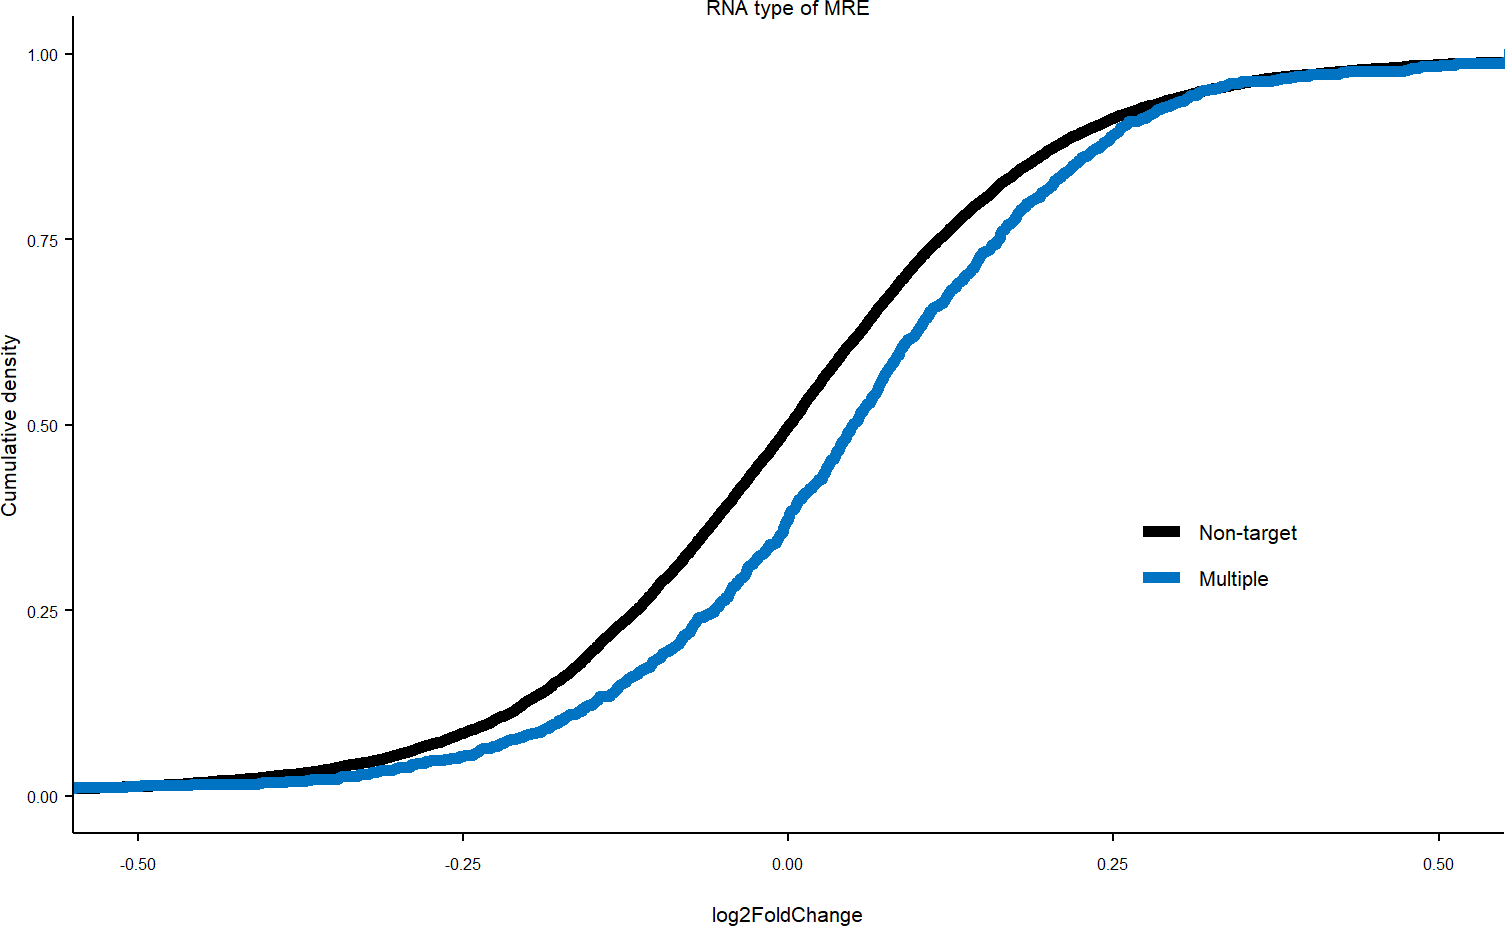
\includegraphics{Fig4_2_files/figure-latex/MREtype-1.pdf}

\begin{Shaded}
\begin{Highlighting}[]
\CommentTok{\# zoom}
\NormalTok{typeECDFRNAZ }\OtherTok{\textless{}{-}} \FunctionTok{ggplot}\NormalTok{(RNA, }\FunctionTok{aes}\NormalTok{(}\FunctionTok{as.numeric}\NormalTok{(log2FoldChange), }
                              \AttributeTok{colour=}\FunctionTok{factor}\NormalTok{(MREtype, }\AttributeTok{levels =} \FunctionTok{c}\NormalTok{(}\StringTok{"Non{-}target"}\NormalTok{, }\StringTok{"No seed"}\NormalTok{, }\StringTok{"seed\_6mer"}\NormalTok{, }\StringTok{"seed\_7mer\_a1"}\NormalTok{, }\StringTok{"seed\_7mer\_m8"}\NormalTok{, }\StringTok{"seed\_8mer"}\NormalTok{, }\StringTok{"seed\_alt\_38"}\NormalTok{, }\StringTok{"Multiple"}\NormalTok{)))) }\SpecialCharTok{+} 
  \FunctionTok{stat\_ecdf}\NormalTok{(}\AttributeTok{geom=}\StringTok{"step"}\NormalTok{, }\AttributeTok{linewidth=}\DecValTok{2}\SpecialCharTok{*}\NormalTok{zoomfac) }\SpecialCharTok{+}
  \FunctionTok{geom\_vline}\NormalTok{(}\AttributeTok{xintercept =} \DecValTok{0}\NormalTok{, }\AttributeTok{linewidth=}\DecValTok{1}\NormalTok{, }\AttributeTok{linetype=}\StringTok{"dashed"}\NormalTok{, }\AttributeTok{colour=}\NormalTok{farbeneg) }\SpecialCharTok{+}
  \FunctionTok{scale\_colour\_manual}\NormalTok{(}\AttributeTok{values =} \FunctionTok{c}\NormalTok{(}\StringTok{"black"}\NormalTok{, farbe1, farbe2, farbe3, farbe4, farbe5, farbe6, farbe7)) }\SpecialCharTok{+}
  \FunctionTok{coord\_cartesian}\NormalTok{(}\AttributeTok{xlim =} \FunctionTok{c}\NormalTok{(}\SpecialCharTok{{-}}\NormalTok{(xlim}\SpecialCharTok{/}\DecValTok{8}\NormalTok{), (xlim}\SpecialCharTok{/}\DecValTok{8}\NormalTok{)), }\AttributeTok{ylim =} \FunctionTok{c}\NormalTok{(}\FloatTok{0.5}\DecValTok{{-}1}\SpecialCharTok{/}\DecValTok{16}\NormalTok{, }\FloatTok{0.5}\SpecialCharTok{+}\DecValTok{1}\SpecialCharTok{/}\DecValTok{16}\NormalTok{)) }\SpecialCharTok{+} 
  \FunctionTok{theme\_bw}\NormalTok{() }\SpecialCharTok{+}
  \FunctionTok{theme}\NormalTok{(}\AttributeTok{legend.position =} \StringTok{"none"}\NormalTok{, }\AttributeTok{axis.text =} \FunctionTok{element\_blank}\NormalTok{(), }\AttributeTok{panel.grid =} \FunctionTok{element\_blank}\NormalTok{(),}
        \AttributeTok{panel.background =} \FunctionTok{element\_rect}\NormalTok{(}\AttributeTok{fill=}\StringTok{\textquotesingle{}transparent\textquotesingle{}}\NormalTok{), }\CommentTok{\#transparent panel bg}
        \AttributeTok{plot.background =} \FunctionTok{element\_rect}\NormalTok{(}\AttributeTok{fill=}\StringTok{\textquotesingle{}transparent\textquotesingle{}}\NormalTok{, }\AttributeTok{color=}\ConstantTok{NA}\NormalTok{)) }\SpecialCharTok{+}
  \FunctionTok{scale\_y\_continuous}\NormalTok{(}\StringTok{""}\NormalTok{) }\SpecialCharTok{+} \FunctionTok{scale\_x\_continuous}\NormalTok{(}\StringTok{""}\NormalTok{)}

\NormalTok{typeECDFRNAZ}
\end{Highlighting}
\end{Shaded}

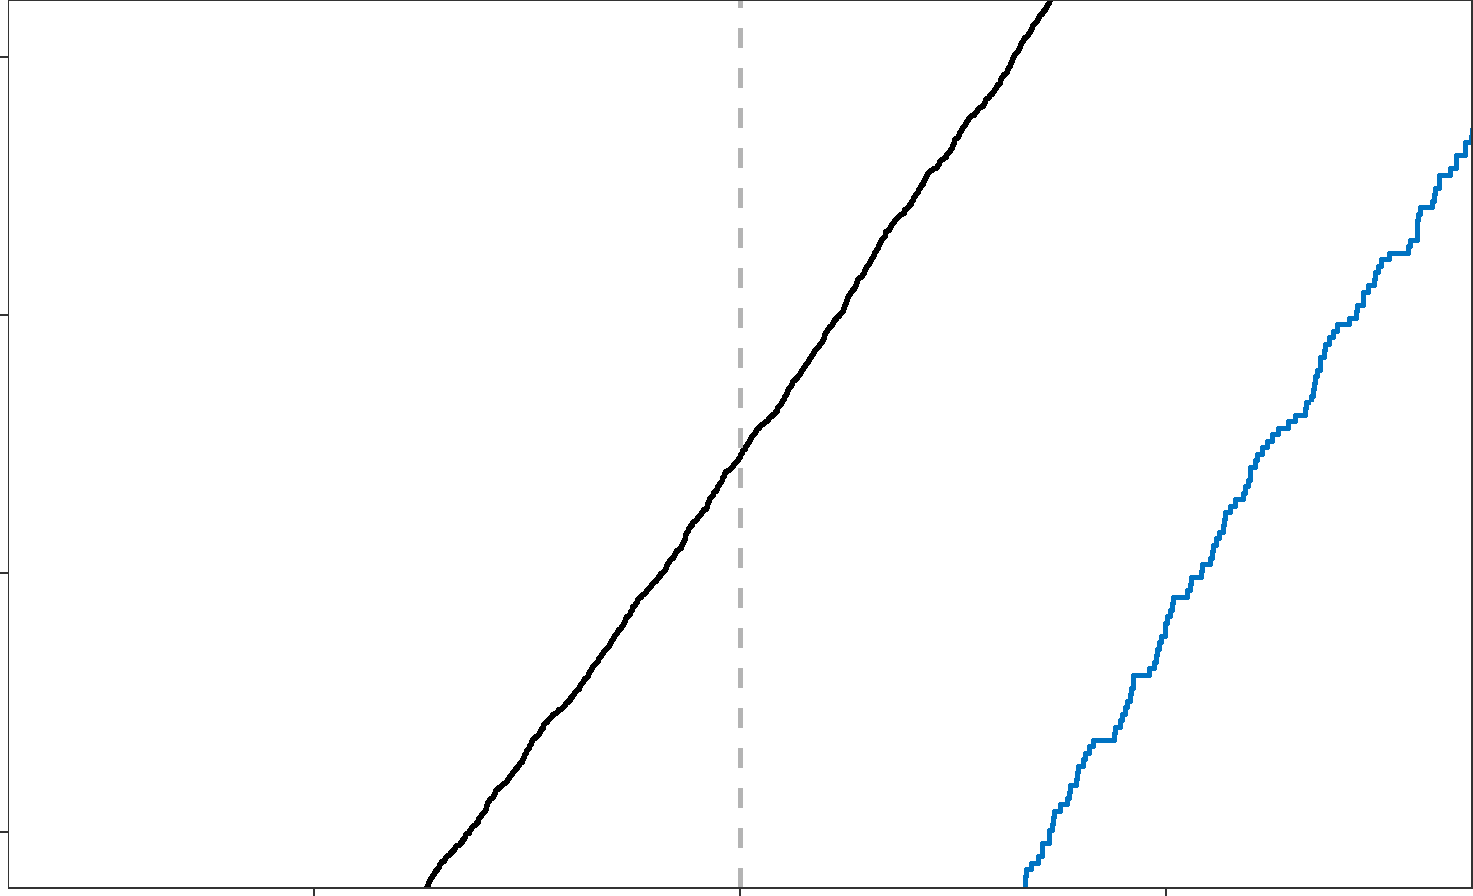
\includegraphics{Fig4_2_files/figure-latex/MREtype-2.pdf}

\begin{Shaded}
\begin{Highlighting}[]
\CommentTok{\#RPF}
\NormalTok{typeECDFRPF }\OtherTok{\textless{}{-}} \FunctionTok{ggplot}\NormalTok{(RPF, }\FunctionTok{aes}\NormalTok{(}\FunctionTok{as.numeric}\NormalTok{(log2FoldChange), }
                              \AttributeTok{colour=}\FunctionTok{factor}\NormalTok{(MREtype, }\AttributeTok{levels =} \FunctionTok{c}\NormalTok{(}\StringTok{"Non{-}target"}\NormalTok{, }\StringTok{"No seed"}\NormalTok{, }\StringTok{"seed\_6mer"}\NormalTok{, }\StringTok{"seed\_7mer\_a1"}\NormalTok{, }\StringTok{"seed\_7mer\_m8"}\NormalTok{, }\StringTok{"seed\_8mer"}\NormalTok{, }\StringTok{"seed\_alt\_38"}\NormalTok{, }\StringTok{"Multiple"}\NormalTok{)))) }\SpecialCharTok{+} 
  \FunctionTok{stat\_ecdf}\NormalTok{(}\AttributeTok{geom=}\StringTok{"step"}\NormalTok{, }\AttributeTok{linewidth=}\DecValTok{2}\NormalTok{) }\SpecialCharTok{+}
  \FunctionTok{geom\_vline}\NormalTok{(}\AttributeTok{xintercept =} \DecValTok{0}\NormalTok{, }\AttributeTok{linewidth=}\DecValTok{1}\NormalTok{, }\AttributeTok{linetype=}\StringTok{"dashed"}\NormalTok{, }\AttributeTok{colour=}\NormalTok{farbeneg) }\SpecialCharTok{+}
  \FunctionTok{scale\_colour\_manual}\NormalTok{(}\AttributeTok{values =} \FunctionTok{c}\NormalTok{(}\StringTok{"black"}\NormalTok{, farbe1, farbe2, farbe3, farbe4, farbe5, farbe6, farbe7)) }\SpecialCharTok{+}
  \FunctionTok{coord\_cartesian}\NormalTok{(}\AttributeTok{xlim =} \FunctionTok{c}\NormalTok{(}\SpecialCharTok{{-}}\NormalTok{xlim, xlim)) }\SpecialCharTok{+} 
  \FunctionTok{theme\_paper}\NormalTok{() }\SpecialCharTok{+}
  \FunctionTok{scale\_y\_continuous}\NormalTok{(}\StringTok{"Cumulative density"}\NormalTok{) }\SpecialCharTok{+} \FunctionTok{scale\_x\_continuous}\NormalTok{(}\StringTok{"log2FoldChange"}\NormalTok{) }\SpecialCharTok{+}
  \FunctionTok{ggtitle}\NormalTok{(}\StringTok{"RPF type of MRE"}\NormalTok{)}

\NormalTok{typeECDFRPF}
\end{Highlighting}
\end{Shaded}

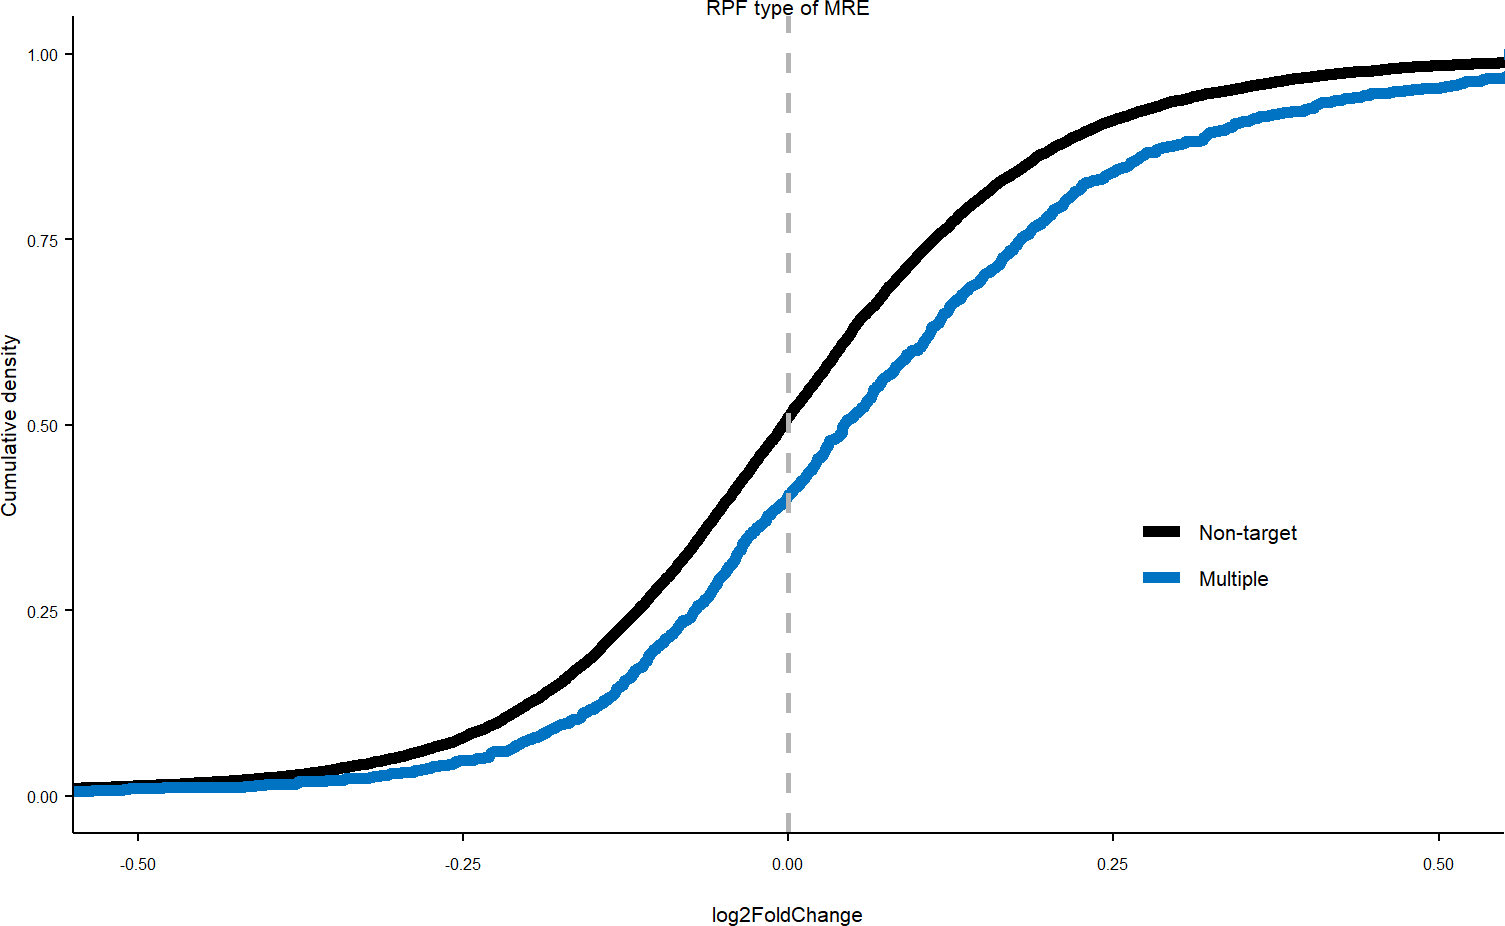
\includegraphics{Fig4_2_files/figure-latex/MREtype-3.pdf}

\begin{Shaded}
\begin{Highlighting}[]
\CommentTok{\# zoom}
\NormalTok{typeECDFRPFZ }\OtherTok{\textless{}{-}} \FunctionTok{ggplot}\NormalTok{(RPF, }\FunctionTok{aes}\NormalTok{(}\FunctionTok{as.numeric}\NormalTok{(log2FoldChange), }
                              \AttributeTok{colour=}\FunctionTok{factor}\NormalTok{(MREtype, }\AttributeTok{levels =} \FunctionTok{c}\NormalTok{(}\StringTok{"Non{-}target"}\NormalTok{, }\StringTok{"No seed"}\NormalTok{, }\StringTok{"seed\_6mer"}\NormalTok{, }\StringTok{"seed\_7mer\_a1"}\NormalTok{, }\StringTok{"seed\_7mer\_m8"}\NormalTok{, }\StringTok{"seed\_8mer"}\NormalTok{, }\StringTok{"seed\_alt\_38"}\NormalTok{, }\StringTok{"Multiple"}\NormalTok{)))) }\SpecialCharTok{+} 
  \FunctionTok{stat\_ecdf}\NormalTok{(}\AttributeTok{geom=}\StringTok{"step"}\NormalTok{, }\AttributeTok{linewidth=}\DecValTok{2}\SpecialCharTok{*}\NormalTok{zoomfac) }\SpecialCharTok{+}
  \FunctionTok{geom\_vline}\NormalTok{(}\AttributeTok{xintercept =} \DecValTok{0}\NormalTok{, }\AttributeTok{linewidth=}\DecValTok{1}\NormalTok{, }\AttributeTok{linetype=}\StringTok{"dashed"}\NormalTok{, }\AttributeTok{colour=}\NormalTok{farbeneg) }\SpecialCharTok{+}
  \FunctionTok{scale\_colour\_manual}\NormalTok{(}\AttributeTok{values =} \FunctionTok{c}\NormalTok{(}\StringTok{"black"}\NormalTok{, farbe1, farbe2, farbe3, farbe4, farbe5, farbe6, farbe7)) }\SpecialCharTok{+}
  \FunctionTok{coord\_cartesian}\NormalTok{(}\AttributeTok{xlim =} \FunctionTok{c}\NormalTok{(}\SpecialCharTok{{-}}\NormalTok{(xlim}\SpecialCharTok{/}\DecValTok{8}\NormalTok{), (xlim}\SpecialCharTok{/}\DecValTok{8}\NormalTok{)), }\AttributeTok{ylim =} \FunctionTok{c}\NormalTok{(}\FloatTok{0.5}\DecValTok{{-}1}\SpecialCharTok{/}\DecValTok{16}\NormalTok{, }\FloatTok{0.5}\SpecialCharTok{+}\DecValTok{1}\SpecialCharTok{/}\DecValTok{16}\NormalTok{)) }\SpecialCharTok{+} 
  \FunctionTok{theme\_bw}\NormalTok{() }\SpecialCharTok{+}
  \FunctionTok{theme}\NormalTok{(}\AttributeTok{legend.position =} \StringTok{"none"}\NormalTok{, }\AttributeTok{axis.text =} \FunctionTok{element\_blank}\NormalTok{(), }\AttributeTok{panel.grid =} \FunctionTok{element\_blank}\NormalTok{(),}
        \AttributeTok{panel.background =} \FunctionTok{element\_rect}\NormalTok{(}\AttributeTok{fill=}\StringTok{\textquotesingle{}transparent\textquotesingle{}}\NormalTok{), }\CommentTok{\#transparent panel bg}
        \AttributeTok{plot.background =} \FunctionTok{element\_rect}\NormalTok{(}\AttributeTok{fill=}\StringTok{\textquotesingle{}transparent\textquotesingle{}}\NormalTok{, }\AttributeTok{color=}\ConstantTok{NA}\NormalTok{)) }\SpecialCharTok{+}
  \FunctionTok{scale\_y\_continuous}\NormalTok{(}\StringTok{""}\NormalTok{) }\SpecialCharTok{+} \FunctionTok{scale\_x\_continuous}\NormalTok{(}\StringTok{""}\NormalTok{)}

\NormalTok{typeECDFRPFZ}
\end{Highlighting}
\end{Shaded}

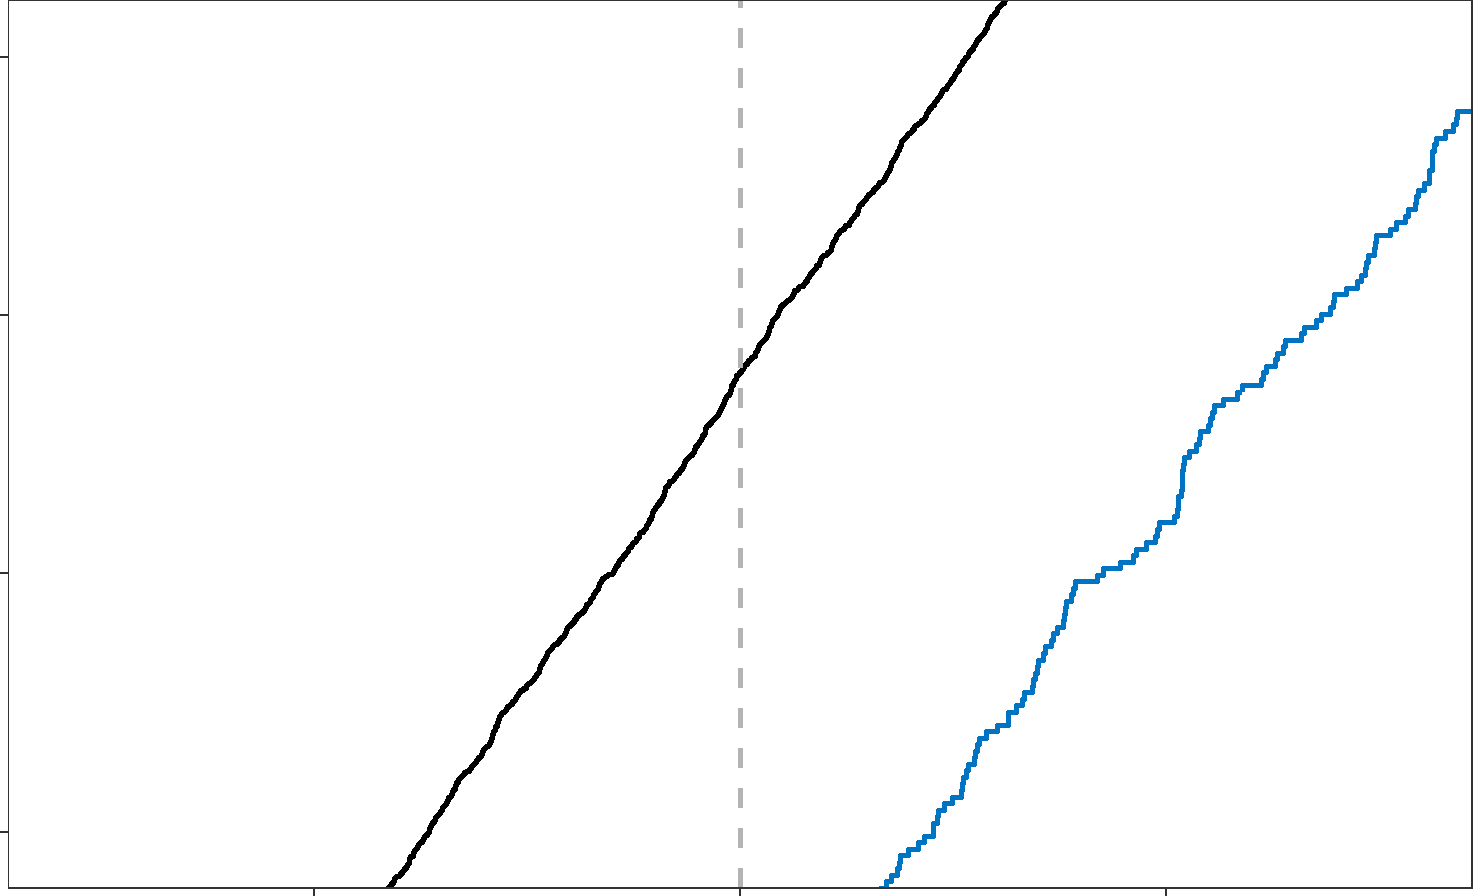
\includegraphics{Fig4_2_files/figure-latex/MREtype-4.pdf}

\begin{Shaded}
\begin{Highlighting}[]
\CommentTok{\#MS}
\NormalTok{typeECDFMS }\OtherTok{\textless{}{-}} \FunctionTok{ggplot}\NormalTok{(MS, }\FunctionTok{aes}\NormalTok{(}\FunctionTok{as.numeric}\NormalTok{(log2FoldChange), }
                              \AttributeTok{colour=}\FunctionTok{factor}\NormalTok{(MREtype, }\AttributeTok{levels =} \FunctionTok{c}\NormalTok{(}\StringTok{"Non{-}target"}\NormalTok{, }\StringTok{"No seed"}\NormalTok{, }\StringTok{"seed\_6mer"}\NormalTok{, }\StringTok{"seed\_7mer\_a1"}\NormalTok{, }\StringTok{"seed\_7mer\_m8"}\NormalTok{, }\StringTok{"seed\_8mer"}\NormalTok{, }\StringTok{"seed\_alt\_38"}\NormalTok{, }\StringTok{"Multiple"}\NormalTok{)))) }\SpecialCharTok{+} 
  \FunctionTok{stat\_ecdf}\NormalTok{(}\AttributeTok{geom=}\StringTok{"step"}\NormalTok{, }\AttributeTok{linewidth=}\DecValTok{2}\NormalTok{) }\SpecialCharTok{+}
  \FunctionTok{geom\_vline}\NormalTok{(}\AttributeTok{xintercept =} \DecValTok{0}\NormalTok{, }\AttributeTok{linewidth=}\DecValTok{1}\NormalTok{, }\AttributeTok{linetype=}\StringTok{"dashed"}\NormalTok{, }\AttributeTok{colour=}\NormalTok{farbeneg) }\SpecialCharTok{+}
  \FunctionTok{scale\_colour\_manual}\NormalTok{(}\AttributeTok{values =} \FunctionTok{c}\NormalTok{(}\StringTok{"black"}\NormalTok{, farbe1, farbe2, farbe3, farbe4, farbe5, farbe6, farbe7)) }\SpecialCharTok{+}
  \FunctionTok{coord\_cartesian}\NormalTok{(}\AttributeTok{xlim =} \FunctionTok{c}\NormalTok{(}\SpecialCharTok{{-}}\NormalTok{xlim, xlim)) }\SpecialCharTok{+} 
  \FunctionTok{theme\_paper}\NormalTok{() }\SpecialCharTok{+}
  \FunctionTok{scale\_y\_continuous}\NormalTok{(}\StringTok{"Cumulative density"}\NormalTok{) }\SpecialCharTok{+} \FunctionTok{scale\_x\_continuous}\NormalTok{(}\StringTok{"log2FoldChange"}\NormalTok{) }\SpecialCharTok{+}
  \FunctionTok{ggtitle}\NormalTok{(}\StringTok{"MS type of MRE"}\NormalTok{)}

\NormalTok{typeECDFMS}
\end{Highlighting}
\end{Shaded}

\begin{verbatim}
## Warning: Removed 712 rows containing non-finite values (`stat_ecdf()`).
\end{verbatim}

\includegraphics{Fig4_2_files/figure-latex/MREtype-5.pdf}

\begin{Shaded}
\begin{Highlighting}[]
\CommentTok{\# zoom}
\NormalTok{typeECDFMSZ }\OtherTok{\textless{}{-}} \FunctionTok{ggplot}\NormalTok{(MS, }\FunctionTok{aes}\NormalTok{(}\FunctionTok{as.numeric}\NormalTok{(log2FoldChange), }
                              \AttributeTok{colour=}\FunctionTok{factor}\NormalTok{(MREtype, }\AttributeTok{levels =} \FunctionTok{c}\NormalTok{(}\StringTok{"Non{-}target"}\NormalTok{, }\StringTok{"No seed"}\NormalTok{, }\StringTok{"seed\_6mer"}\NormalTok{, }\StringTok{"seed\_7mer\_a1"}\NormalTok{, }\StringTok{"seed\_7mer\_m8"}\NormalTok{, }\StringTok{"seed\_8mer"}\NormalTok{, }\StringTok{"seed\_alt\_38"}\NormalTok{, }\StringTok{"Multiple"}\NormalTok{)))) }\SpecialCharTok{+} 
  \FunctionTok{stat\_ecdf}\NormalTok{(}\AttributeTok{geom=}\StringTok{"step"}\NormalTok{, }\AttributeTok{linewidth=}\DecValTok{2}\SpecialCharTok{*}\NormalTok{zoomfac) }\SpecialCharTok{+}
  \FunctionTok{geom\_vline}\NormalTok{(}\AttributeTok{xintercept =} \DecValTok{0}\NormalTok{, }\AttributeTok{linewidth=}\DecValTok{1}\NormalTok{, }\AttributeTok{linetype=}\StringTok{"dashed"}\NormalTok{, }\AttributeTok{colour=}\NormalTok{farbeneg) }\SpecialCharTok{+}
  \FunctionTok{scale\_colour\_manual}\NormalTok{(}\AttributeTok{values =} \FunctionTok{c}\NormalTok{(}\StringTok{"black"}\NormalTok{, farbe1, farbe2, farbe3, farbe4, farbe5, farbe6, farbe7)) }\SpecialCharTok{+}
  \FunctionTok{coord\_cartesian}\NormalTok{(}\AttributeTok{xlim =} \FunctionTok{c}\NormalTok{(}\SpecialCharTok{{-}}\NormalTok{(xlim}\SpecialCharTok{/}\DecValTok{8}\NormalTok{), (xlim}\SpecialCharTok{/}\DecValTok{8}\NormalTok{)), }\AttributeTok{ylim =} \FunctionTok{c}\NormalTok{(}\FloatTok{0.5}\DecValTok{{-}1}\SpecialCharTok{/}\DecValTok{16}\NormalTok{, }\FloatTok{0.5}\SpecialCharTok{+}\DecValTok{1}\SpecialCharTok{/}\DecValTok{16}\NormalTok{)) }\SpecialCharTok{+} 
  \FunctionTok{theme\_bw}\NormalTok{() }\SpecialCharTok{+}
  \FunctionTok{theme}\NormalTok{(}\AttributeTok{legend.position =} \StringTok{"none"}\NormalTok{, }\AttributeTok{axis.text =} \FunctionTok{element\_blank}\NormalTok{(), }\AttributeTok{panel.grid =} \FunctionTok{element\_blank}\NormalTok{(),}
        \AttributeTok{panel.background =} \FunctionTok{element\_rect}\NormalTok{(}\AttributeTok{fill=}\StringTok{\textquotesingle{}transparent\textquotesingle{}}\NormalTok{), }\CommentTok{\#transparent panel bg}
        \AttributeTok{plot.background =} \FunctionTok{element\_rect}\NormalTok{(}\AttributeTok{fill=}\StringTok{\textquotesingle{}transparent\textquotesingle{}}\NormalTok{, }\AttributeTok{color=}\ConstantTok{NA}\NormalTok{)) }\SpecialCharTok{+}
  \FunctionTok{scale\_y\_continuous}\NormalTok{(}\StringTok{""}\NormalTok{) }\SpecialCharTok{+} \FunctionTok{scale\_x\_continuous}\NormalTok{(}\StringTok{""}\NormalTok{)}

\NormalTok{typeECDFMSZ}
\end{Highlighting}
\end{Shaded}

\begin{verbatim}
## Warning: Removed 712 rows containing non-finite values (`stat_ecdf()`).
\end{verbatim}

\includegraphics{Fig4_2_files/figure-latex/MREtype-6.pdf}

\begin{Shaded}
\begin{Highlighting}[]
\CommentTok{\#TE}
\NormalTok{typeECDFTE }\OtherTok{\textless{}{-}} \FunctionTok{ggplot}\NormalTok{(TE, }\FunctionTok{aes}\NormalTok{(}\FunctionTok{as.numeric}\NormalTok{(log2FoldChange), }
                              \AttributeTok{colour=}\FunctionTok{factor}\NormalTok{(MREtype, }\AttributeTok{levels =} \FunctionTok{c}\NormalTok{(}\StringTok{"Non{-}target"}\NormalTok{, }\StringTok{"No seed"}\NormalTok{, }\StringTok{"seed\_6mer"}\NormalTok{, }\StringTok{"seed\_7mer\_a1"}\NormalTok{, }\StringTok{"seed\_7mer\_m8"}\NormalTok{, }\StringTok{"seed\_8mer"}\NormalTok{, }\StringTok{"seed\_alt\_38"}\NormalTok{, }\StringTok{"Multiple"}\NormalTok{)))) }\SpecialCharTok{+} 
  \FunctionTok{stat\_ecdf}\NormalTok{(}\AttributeTok{geom=}\StringTok{"step"}\NormalTok{, }\AttributeTok{linewidth=}\DecValTok{2}\NormalTok{) }\SpecialCharTok{+}
  \FunctionTok{geom\_vline}\NormalTok{(}\AttributeTok{xintercept =} \DecValTok{0}\NormalTok{, }\AttributeTok{linewidth=}\DecValTok{1}\NormalTok{, }\AttributeTok{linetype=}\StringTok{"dashed"}\NormalTok{, }\AttributeTok{colour=}\NormalTok{farbeneg) }\SpecialCharTok{+}
  \FunctionTok{scale\_colour\_manual}\NormalTok{(}\AttributeTok{values =} \FunctionTok{c}\NormalTok{(}\StringTok{"black"}\NormalTok{, farbe1, farbe2, farbe3, farbe4, farbe5, farbe6, farbe7)) }\SpecialCharTok{+}
  \FunctionTok{coord\_cartesian}\NormalTok{(}\AttributeTok{xlim =} \FunctionTok{c}\NormalTok{(}\SpecialCharTok{{-}}\NormalTok{xlim, xlim)) }\SpecialCharTok{+} 
  \FunctionTok{theme\_paper}\NormalTok{() }\SpecialCharTok{+}
  \FunctionTok{scale\_y\_continuous}\NormalTok{(}\StringTok{"Cumulative density"}\NormalTok{) }\SpecialCharTok{+} \FunctionTok{scale\_x\_continuous}\NormalTok{(}\StringTok{"log2FoldChange"}\NormalTok{) }\SpecialCharTok{+}
  \FunctionTok{ggtitle}\NormalTok{(}\StringTok{"TE type of MRE"}\NormalTok{)}

\NormalTok{typeECDFTE}
\end{Highlighting}
\end{Shaded}

\includegraphics{Fig4_2_files/figure-latex/MREtype-7.pdf}

\begin{Shaded}
\begin{Highlighting}[]
\CommentTok{\# zoom}
\NormalTok{typeECDFTEZ }\OtherTok{\textless{}{-}} \FunctionTok{ggplot}\NormalTok{(TE, }\FunctionTok{aes}\NormalTok{(}\FunctionTok{as.numeric}\NormalTok{(log2FoldChange), }
                              \AttributeTok{colour=}\FunctionTok{factor}\NormalTok{(MREtype, }\AttributeTok{levels =} \FunctionTok{c}\NormalTok{(}\StringTok{"Non{-}target"}\NormalTok{, }\StringTok{"No seed"}\NormalTok{, }\StringTok{"seed\_6mer"}\NormalTok{, }\StringTok{"seed\_7mer\_a1"}\NormalTok{, }\StringTok{"seed\_7mer\_m8"}\NormalTok{, }\StringTok{"seed\_8mer"}\NormalTok{, }\StringTok{"seed\_alt\_38"}\NormalTok{, }\StringTok{"Multiple"}\NormalTok{)))) }\SpecialCharTok{+} 
  \FunctionTok{stat\_ecdf}\NormalTok{(}\AttributeTok{geom=}\StringTok{"step"}\NormalTok{, }\AttributeTok{linewidth=}\DecValTok{2}\SpecialCharTok{*}\NormalTok{zoomfac) }\SpecialCharTok{+}
  \FunctionTok{geom\_vline}\NormalTok{(}\AttributeTok{xintercept =} \DecValTok{0}\NormalTok{, }\AttributeTok{linewidth=}\DecValTok{1}\NormalTok{, }\AttributeTok{linetype=}\StringTok{"dashed"}\NormalTok{, }\AttributeTok{colour=}\NormalTok{farbeneg) }\SpecialCharTok{+}
  \FunctionTok{scale\_colour\_manual}\NormalTok{(}\AttributeTok{values =} \FunctionTok{c}\NormalTok{(}\StringTok{"black"}\NormalTok{, farbe1, farbe2, farbe3, farbe4, farbe5, farbe6, farbe7)) }\SpecialCharTok{+}
  \FunctionTok{coord\_cartesian}\NormalTok{(}\AttributeTok{xlim =} \FunctionTok{c}\NormalTok{(}\SpecialCharTok{{-}}\NormalTok{(xlim}\SpecialCharTok{/}\DecValTok{8}\NormalTok{), (xlim}\SpecialCharTok{/}\DecValTok{8}\NormalTok{)), }\AttributeTok{ylim =} \FunctionTok{c}\NormalTok{(}\FloatTok{0.5}\DecValTok{{-}1}\SpecialCharTok{/}\DecValTok{16}\NormalTok{, }\FloatTok{0.5}\SpecialCharTok{+}\DecValTok{1}\SpecialCharTok{/}\DecValTok{16}\NormalTok{)) }\SpecialCharTok{+} 
  \FunctionTok{theme\_bw}\NormalTok{() }\SpecialCharTok{+}
  \FunctionTok{theme}\NormalTok{(}\AttributeTok{legend.position =} \StringTok{"none"}\NormalTok{, }\AttributeTok{axis.text =} \FunctionTok{element\_blank}\NormalTok{(), }\AttributeTok{panel.grid =} \FunctionTok{element\_blank}\NormalTok{(),}
        \AttributeTok{panel.background =} \FunctionTok{element\_rect}\NormalTok{(}\AttributeTok{fill=}\StringTok{\textquotesingle{}transparent\textquotesingle{}}\NormalTok{), }\CommentTok{\#transparent panel bg}
        \AttributeTok{plot.background =} \FunctionTok{element\_rect}\NormalTok{(}\AttributeTok{fill=}\StringTok{\textquotesingle{}transparent\textquotesingle{}}\NormalTok{, }\AttributeTok{color=}\ConstantTok{NA}\NormalTok{)) }\SpecialCharTok{+}
  \FunctionTok{scale\_y\_continuous}\NormalTok{(}\StringTok{""}\NormalTok{) }\SpecialCharTok{+} \FunctionTok{scale\_x\_continuous}\NormalTok{(}\StringTok{""}\NormalTok{)}

\NormalTok{typeECDFTEZ}
\end{Highlighting}
\end{Shaded}

\includegraphics{Fig4_2_files/figure-latex/MREtype-8.pdf}

\begin{Shaded}
\begin{Highlighting}[]
\CommentTok{\#export RNA}
\FunctionTok{pdf}\NormalTok{(}\StringTok{"C:/Users/nikit/Documents/Krueger\_Lab/Publications/miR181\_paper/Figure4/typeECDF\_RNA.pdf"}\NormalTok{, }\AttributeTok{width=}\DecValTok{2}\NormalTok{, }\AttributeTok{height =} \DecValTok{2}\NormalTok{)}
\NormalTok{typeECDFRNA}
\FunctionTok{dev.off}\NormalTok{()}
\end{Highlighting}
\end{Shaded}

\begin{verbatim}
## pdf 
##   2
\end{verbatim}

\begin{Shaded}
\begin{Highlighting}[]
\FunctionTok{pdf}\NormalTok{(}\StringTok{"C:/Users/nikit/Documents/Krueger\_Lab/Publications/miR181\_paper/Figure4/typeECDF\_RNA\_zoom.pdf"}\NormalTok{, }\AttributeTok{width=}\DecValTok{2}\SpecialCharTok{*}\NormalTok{zoomfac, }\AttributeTok{height =} \DecValTok{2}\SpecialCharTok{*}\NormalTok{zoomfac)}
\NormalTok{typeECDFRNAZ}
\FunctionTok{dev.off}\NormalTok{()}
\end{Highlighting}
\end{Shaded}

\begin{verbatim}
## pdf 
##   2
\end{verbatim}

\begin{Shaded}
\begin{Highlighting}[]
\CommentTok{\#export RPF}
\FunctionTok{pdf}\NormalTok{(}\StringTok{"C:/Users/nikit/Documents/Krueger\_Lab/Publications/miR181\_paper/Figure4/typeECDF\_RPF.pdf"}\NormalTok{, }\AttributeTok{width=}\DecValTok{2}\NormalTok{, }\AttributeTok{height =} \DecValTok{2}\NormalTok{)}
\NormalTok{typeECDFRPF}
\FunctionTok{dev.off}\NormalTok{()}
\end{Highlighting}
\end{Shaded}

\begin{verbatim}
## pdf 
##   2
\end{verbatim}

\begin{Shaded}
\begin{Highlighting}[]
\FunctionTok{pdf}\NormalTok{(}\StringTok{"C:/Users/nikit/Documents/Krueger\_Lab/Publications/miR181\_paper/Figure4/typeECDF\_RPF\_zoom.pdf"}\NormalTok{, }\AttributeTok{width=}\DecValTok{2}\SpecialCharTok{*}\NormalTok{zoomfac, }\AttributeTok{height =} \DecValTok{2}\SpecialCharTok{*}\NormalTok{zoomfac)}
\NormalTok{typeECDFRPFZ}
\FunctionTok{dev.off}\NormalTok{()}
\end{Highlighting}
\end{Shaded}

\begin{verbatim}
## pdf 
##   2
\end{verbatim}

\begin{Shaded}
\begin{Highlighting}[]
\CommentTok{\#export MS}
\FunctionTok{pdf}\NormalTok{(}\StringTok{"C:/Users/nikit/Documents/Krueger\_Lab/Publications/miR181\_paper/Figure4/typeECDF\_MS.pdf"}\NormalTok{, }\AttributeTok{width=}\DecValTok{2}\NormalTok{, }\AttributeTok{height =} \DecValTok{2}\NormalTok{)}
\NormalTok{typeECDFMS}
\end{Highlighting}
\end{Shaded}

\begin{verbatim}
## Warning: Removed 712 rows containing non-finite values (`stat_ecdf()`).
\end{verbatim}

\begin{Shaded}
\begin{Highlighting}[]
\FunctionTok{dev.off}\NormalTok{()}
\end{Highlighting}
\end{Shaded}

\begin{verbatim}
## pdf 
##   2
\end{verbatim}

\begin{Shaded}
\begin{Highlighting}[]
\FunctionTok{pdf}\NormalTok{(}\StringTok{"C:/Users/nikit/Documents/Krueger\_Lab/Publications/miR181\_paper/Figure4/typeECDF\_MS\_zoom.pdf"}\NormalTok{, }\AttributeTok{width=}\DecValTok{2}\SpecialCharTok{*}\NormalTok{zoomfac, }\AttributeTok{height =} \DecValTok{2}\SpecialCharTok{*}\NormalTok{zoomfac)}
\NormalTok{typeECDFMSZ}
\end{Highlighting}
\end{Shaded}

\begin{verbatim}
## Warning: Removed 712 rows containing non-finite values (`stat_ecdf()`).
\end{verbatim}

\begin{Shaded}
\begin{Highlighting}[]
\FunctionTok{dev.off}\NormalTok{()}
\end{Highlighting}
\end{Shaded}

\begin{verbatim}
## pdf 
##   2
\end{verbatim}

\begin{Shaded}
\begin{Highlighting}[]
\CommentTok{\#export TE}
\FunctionTok{pdf}\NormalTok{(}\StringTok{"C:/Users/nikit/Documents/Krueger\_Lab/Publications/miR181\_paper/Figure4/typeECDF\_TE.pdf"}\NormalTok{, }\AttributeTok{width=}\DecValTok{2}\NormalTok{, }\AttributeTok{height =} \DecValTok{2}\NormalTok{)}
\NormalTok{typeECDFTE}
\FunctionTok{dev.off}\NormalTok{()}
\end{Highlighting}
\end{Shaded}

\begin{verbatim}
## pdf 
##   2
\end{verbatim}

\begin{Shaded}
\begin{Highlighting}[]
\FunctionTok{pdf}\NormalTok{(}\StringTok{"C:/Users/nikit/Documents/Krueger\_Lab/Publications/miR181\_paper/Figure4/typeECDF\_TE\_zoom.pdf"}\NormalTok{, }\AttributeTok{width=}\DecValTok{2}\SpecialCharTok{*}\NormalTok{zoomfac, }\AttributeTok{height =} \DecValTok{2}\SpecialCharTok{*}\NormalTok{zoomfac)}
\NormalTok{typeECDFTEZ}
\FunctionTok{dev.off}\NormalTok{()}
\end{Highlighting}
\end{Shaded}

\begin{verbatim}
## pdf 
##   2
\end{verbatim}

\begin{Shaded}
\begin{Highlighting}[]
\FunctionTok{table}\NormalTok{(RPF}\SpecialCharTok{$}\NormalTok{MREtype)}
\end{Highlighting}
\end{Shaded}

\begin{verbatim}
## 
##     Multiple      No seed   Non-target    seed_6mer seed_7mer_a1 seed_7mer_m8 
##          990          713         9222          121           53          103 
##    seed_8mer  seed_alt_38 
##           75           92
\end{verbatim}

\hypertarget{te-density-type}{%
\section{TE density type}\label{te-density-type}}

\begin{Shaded}
\begin{Highlighting}[]
\NormalTok{TEdenstyp }\OtherTok{\textless{}{-}} \FunctionTok{ggplot}\NormalTok{(TE, }\FunctionTok{aes}\NormalTok{(}\AttributeTok{x=}\NormalTok{log2FoldChange, }\AttributeTok{colour=}\FunctionTok{factor}\NormalTok{(MREtype, }\AttributeTok{levels =} \FunctionTok{c}\NormalTok{(}\StringTok{"No seed"}\NormalTok{, }\StringTok{"seed\_6mer"}\NormalTok{, }\StringTok{"seed\_7mer\_a1"}\NormalTok{, }\StringTok{"seed\_7mer\_m8"}\NormalTok{, }\StringTok{"seed\_8mer"}\NormalTok{, }\StringTok{"seed\_alt\_38"}\NormalTok{, }\StringTok{"Multiple"}\NormalTok{, }\StringTok{"Non{-}target"}\NormalTok{)))) }\SpecialCharTok{+}
  \FunctionTok{geom\_density}\NormalTok{() }\SpecialCharTok{+}
  \FunctionTok{geom\_vline}\NormalTok{(}\AttributeTok{xintercept =} \DecValTok{0}\NormalTok{, }\AttributeTok{linewidth=}\DecValTok{1}\NormalTok{, }\AttributeTok{linetype=}\StringTok{"dashed"}\NormalTok{, }\AttributeTok{colour=}\NormalTok{farbeneg) }\SpecialCharTok{+}
  \FunctionTok{scale\_colour\_manual}\NormalTok{(}\AttributeTok{values =} \FunctionTok{c}\NormalTok{( farbe1, farbe2, farbe3, farbe4, farbe5, farbe6, farbe7, }\StringTok{"black"}\NormalTok{)) }\SpecialCharTok{+}
  \FunctionTok{theme\_paper}\NormalTok{() }\SpecialCharTok{+}
  \FunctionTok{coord\_cartesian}\NormalTok{(}\AttributeTok{xlim =} \FunctionTok{c}\NormalTok{(}\SpecialCharTok{{-}}\DecValTok{1}\NormalTok{,}\DecValTok{1}\NormalTok{)) }\SpecialCharTok{+}
  \FunctionTok{ggtitle}\NormalTok{(}\StringTok{"TE"}\NormalTok{)}

\NormalTok{TEdenstyp}
\end{Highlighting}
\end{Shaded}

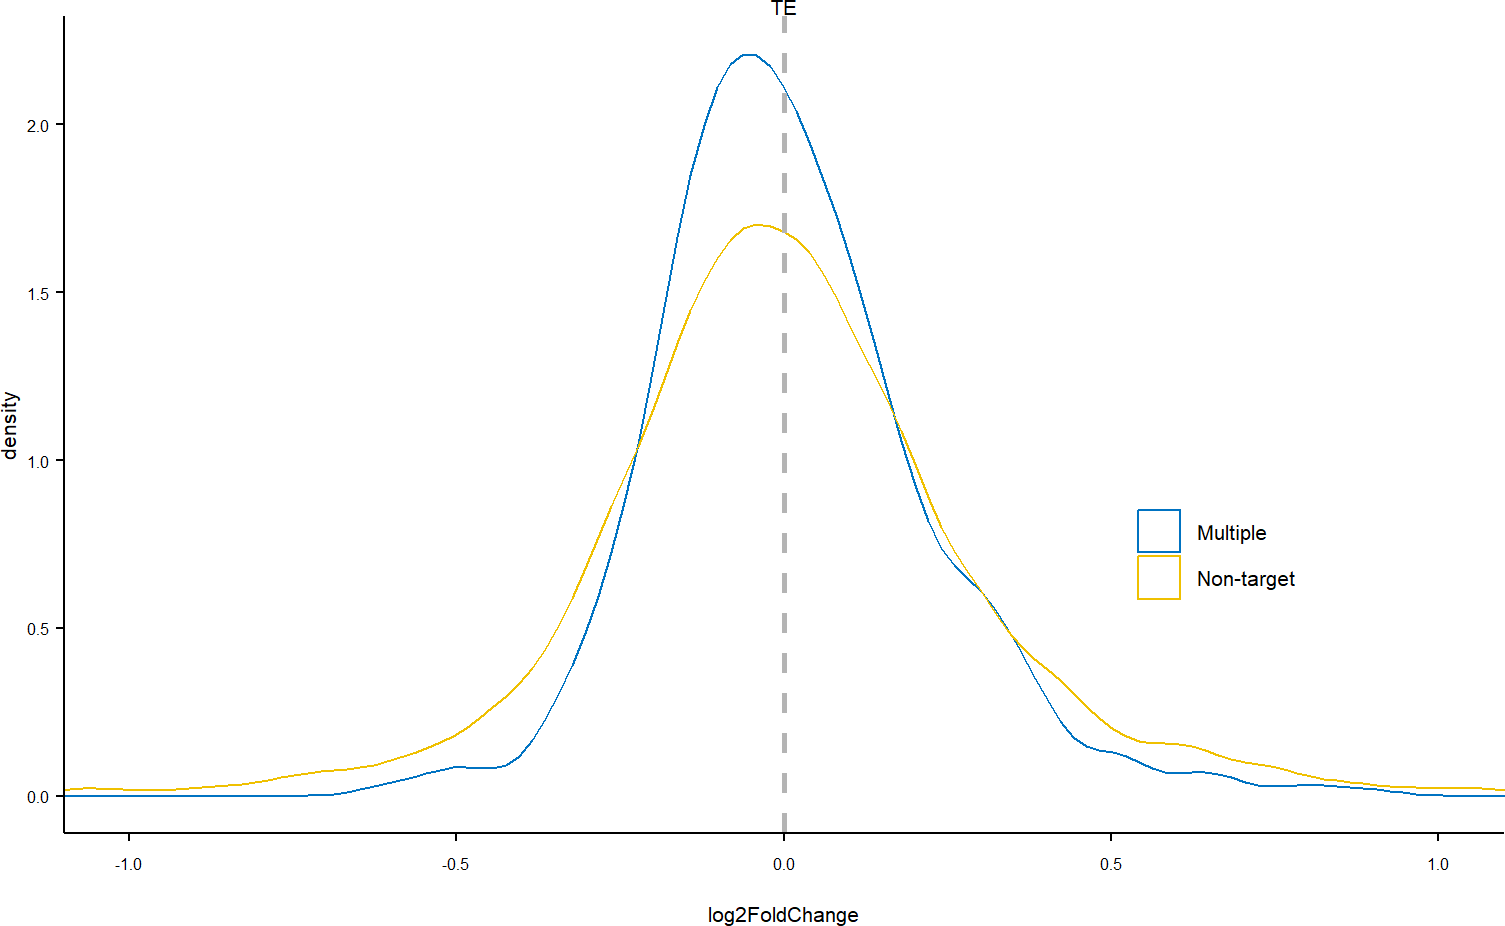
\includegraphics{Fig4_2_files/figure-latex/TEdensitytype-1.pdf}

\begin{Shaded}
\begin{Highlighting}[]
\FunctionTok{pdf}\NormalTok{(}\StringTok{"C:/Users/nikit/Documents/Krueger\_Lab/Publications/miR181\_paper/Figure4/TypeDensity\_TE.pdf"}\NormalTok{, }\AttributeTok{width=}\DecValTok{2}\NormalTok{, }\AttributeTok{height =} \DecValTok{2}\NormalTok{)}
\NormalTok{TEdenstyp}
\FunctionTok{dev.off}\NormalTok{()}
\end{Highlighting}
\end{Shaded}

\begin{verbatim}
## pdf 
##   2
\end{verbatim}

\hypertarget{significance-1}{%
\subsection{Significance}\label{significance-1}}

\begin{Shaded}
\begin{Highlighting}[]
\NormalTok{RNATypeTTest1 }\OtherTok{\textless{}{-}} \FunctionTok{t.test}\NormalTok{(RNA[RNA}\SpecialCharTok{$}\NormalTok{MREtype}\SpecialCharTok{==}\StringTok{"seed\_6mer"}\NormalTok{, }\StringTok{"log2FoldChange"}\NormalTok{], RNA[RNA}\SpecialCharTok{$}\NormalTok{MREtype}\SpecialCharTok{==}\StringTok{"Non{-}target"}\NormalTok{, }\StringTok{"log2FoldChange"}\NormalTok{])}
\NormalTok{RNATypeTTest2 }\OtherTok{\textless{}{-}} \FunctionTok{t.test}\NormalTok{(RNA[RNA}\SpecialCharTok{$}\NormalTok{MREtype}\SpecialCharTok{==}\StringTok{"seed\_7mer\_a1"}\NormalTok{, }\StringTok{"log2FoldChange"}\NormalTok{], RNA[RNA}\SpecialCharTok{$}\NormalTok{MREtype}\SpecialCharTok{==}\StringTok{"Non{-}target"}\NormalTok{, }\StringTok{"log2FoldChange"}\NormalTok{])}
\NormalTok{RNATypeTTest3 }\OtherTok{\textless{}{-}} \FunctionTok{t.test}\NormalTok{(RNA[RNA}\SpecialCharTok{$}\NormalTok{MREtype}\SpecialCharTok{==}\StringTok{"seed\_7mer\_m8"}\NormalTok{, }\StringTok{"log2FoldChange"}\NormalTok{], RNA[RNA}\SpecialCharTok{$}\NormalTok{MREtype}\SpecialCharTok{==}\StringTok{"Non{-}target"}\NormalTok{, }\StringTok{"log2FoldChange"}\NormalTok{])}
\NormalTok{RNATypeTTest4 }\OtherTok{\textless{}{-}} \FunctionTok{t.test}\NormalTok{(RNA[RNA}\SpecialCharTok{$}\NormalTok{MREtype}\SpecialCharTok{==}\StringTok{"seed\_8mer"}\NormalTok{, }\StringTok{"log2FoldChange"}\NormalTok{], RNA[RNA}\SpecialCharTok{$}\NormalTok{MREtype}\SpecialCharTok{==}\StringTok{"Non{-}target"}\NormalTok{, }\StringTok{"log2FoldChange"}\NormalTok{])}
\NormalTok{RNATypeTTest5 }\OtherTok{\textless{}{-}} \FunctionTok{t.test}\NormalTok{(RNA[RNA}\SpecialCharTok{$}\NormalTok{MREtype}\SpecialCharTok{==}\StringTok{"seed\_alt\_38"}\NormalTok{, }\StringTok{"log2FoldChange"}\NormalTok{], RNA[RNA}\SpecialCharTok{$}\NormalTok{MREtype}\SpecialCharTok{==}\StringTok{"Non{-}target"}\NormalTok{, }\StringTok{"log2FoldChange"}\NormalTok{])}

\NormalTok{RPFTypeTTest1 }\OtherTok{\textless{}{-}} \FunctionTok{t.test}\NormalTok{(RPF[RPF}\SpecialCharTok{$}\NormalTok{MREtype}\SpecialCharTok{==}\StringTok{"seed\_6mer"}\NormalTok{, }\StringTok{"log2FoldChange"}\NormalTok{], RPF[RPF}\SpecialCharTok{$}\NormalTok{MREtype}\SpecialCharTok{==}\StringTok{"Non{-}target"}\NormalTok{, }\StringTok{"log2FoldChange"}\NormalTok{])}
\NormalTok{RPFTypeTTest2 }\OtherTok{\textless{}{-}} \FunctionTok{t.test}\NormalTok{(RPF[RPF}\SpecialCharTok{$}\NormalTok{MREtype}\SpecialCharTok{==}\StringTok{"seed\_7mer\_a1"}\NormalTok{, }\StringTok{"log2FoldChange"}\NormalTok{], RPF[RPF}\SpecialCharTok{$}\NormalTok{MREtype}\SpecialCharTok{==}\StringTok{"Non{-}target"}\NormalTok{, }\StringTok{"log2FoldChange"}\NormalTok{])}
\NormalTok{RPFTypeTTest3 }\OtherTok{\textless{}{-}} \FunctionTok{t.test}\NormalTok{(RPF[RPF}\SpecialCharTok{$}\NormalTok{MREtype}\SpecialCharTok{==}\StringTok{"seed\_7mer\_m8"}\NormalTok{, }\StringTok{"log2FoldChange"}\NormalTok{], RPF[RPF}\SpecialCharTok{$}\NormalTok{MREtype}\SpecialCharTok{==}\StringTok{"Non{-}target"}\NormalTok{, }\StringTok{"log2FoldChange"}\NormalTok{])}
\NormalTok{RPFTypeTTest4 }\OtherTok{\textless{}{-}} \FunctionTok{t.test}\NormalTok{(RPF[RPF}\SpecialCharTok{$}\NormalTok{MREtype}\SpecialCharTok{==}\StringTok{"seed\_8mer"}\NormalTok{, }\StringTok{"log2FoldChange"}\NormalTok{], RPF[RPF}\SpecialCharTok{$}\NormalTok{MREtype}\SpecialCharTok{==}\StringTok{"Non{-}target"}\NormalTok{, }\StringTok{"log2FoldChange"}\NormalTok{])}
\NormalTok{RPFTypeTTest5 }\OtherTok{\textless{}{-}} \FunctionTok{t.test}\NormalTok{(RPF[RPF}\SpecialCharTok{$}\NormalTok{MREtype}\SpecialCharTok{==}\StringTok{"seed\_alt\_38"}\NormalTok{, }\StringTok{"log2FoldChange"}\NormalTok{], RPF[RPF}\SpecialCharTok{$}\NormalTok{MREtype}\SpecialCharTok{==}\StringTok{"Non{-}target"}\NormalTok{, }\StringTok{"log2FoldChange"}\NormalTok{])}

\NormalTok{TETypeTTest1 }\OtherTok{\textless{}{-}} \FunctionTok{t.test}\NormalTok{(TE[TE}\SpecialCharTok{$}\NormalTok{MREtype}\SpecialCharTok{==}\StringTok{"seed\_6mer"}\NormalTok{, }\StringTok{"log2FoldChange"}\NormalTok{], TE[TE}\SpecialCharTok{$}\NormalTok{MREtype}\SpecialCharTok{==}\StringTok{"Non{-}target"}\NormalTok{, }\StringTok{"log2FoldChange"}\NormalTok{])}
\NormalTok{TETypeTTest2 }\OtherTok{\textless{}{-}} \FunctionTok{t.test}\NormalTok{(TE[TE}\SpecialCharTok{$}\NormalTok{MREtype}\SpecialCharTok{==}\StringTok{"seed\_7mer\_a1"}\NormalTok{, }\StringTok{"log2FoldChange"}\NormalTok{], TE[TE}\SpecialCharTok{$}\NormalTok{MREtype}\SpecialCharTok{==}\StringTok{"Non{-}target"}\NormalTok{, }\StringTok{"log2FoldChange"}\NormalTok{])}
\NormalTok{TETypeTTest3 }\OtherTok{\textless{}{-}} \FunctionTok{t.test}\NormalTok{(TE[TE}\SpecialCharTok{$}\NormalTok{MREtype}\SpecialCharTok{==}\StringTok{"seed\_7mer\_m8"}\NormalTok{, }\StringTok{"log2FoldChange"}\NormalTok{], TE[TE}\SpecialCharTok{$}\NormalTok{MREtype}\SpecialCharTok{==}\StringTok{"Non{-}target"}\NormalTok{, }\StringTok{"log2FoldChange"}\NormalTok{])}
\NormalTok{TETypeTTest4 }\OtherTok{\textless{}{-}} \FunctionTok{t.test}\NormalTok{(TE[TE}\SpecialCharTok{$}\NormalTok{MREtype}\SpecialCharTok{==}\StringTok{"seed\_8mer"}\NormalTok{, }\StringTok{"log2FoldChange"}\NormalTok{], TE[TE}\SpecialCharTok{$}\NormalTok{MREtype}\SpecialCharTok{==}\StringTok{"Non{-}target"}\NormalTok{, }\StringTok{"log2FoldChange"}\NormalTok{])}
\NormalTok{TETypeTTest5 }\OtherTok{\textless{}{-}} \FunctionTok{t.test}\NormalTok{(TE[TE}\SpecialCharTok{$}\NormalTok{MREtype}\SpecialCharTok{==}\StringTok{"seed\_alt\_38"}\NormalTok{, }\StringTok{"log2FoldChange"}\NormalTok{], TE[TE}\SpecialCharTok{$}\NormalTok{MREtype}\SpecialCharTok{==}\StringTok{"Non{-}target"}\NormalTok{, }\StringTok{"log2FoldChange"}\NormalTok{])}

\NormalTok{MSTypeTTest1 }\OtherTok{\textless{}{-}} \FunctionTok{t.test}\NormalTok{(MS[MS}\SpecialCharTok{$}\NormalTok{MREtype}\SpecialCharTok{==}\StringTok{"seed\_6mer"}\NormalTok{, }\StringTok{"log2FoldChange"}\NormalTok{], MS[MS}\SpecialCharTok{$}\NormalTok{MREtype}\SpecialCharTok{==}\StringTok{"Non{-}target"}\NormalTok{, }\StringTok{"log2FoldChange"}\NormalTok{])}
\NormalTok{MSTypeTTest2 }\OtherTok{\textless{}{-}} \FunctionTok{t.test}\NormalTok{(MS[MS}\SpecialCharTok{$}\NormalTok{MREtype}\SpecialCharTok{==}\StringTok{"seed\_7mer\_a1"}\NormalTok{, }\StringTok{"log2FoldChange"}\NormalTok{], MS[MS}\SpecialCharTok{$}\NormalTok{MREtype}\SpecialCharTok{==}\StringTok{"Non{-}target"}\NormalTok{, }\StringTok{"log2FoldChange"}\NormalTok{])}
\NormalTok{MSTypeTTest3 }\OtherTok{\textless{}{-}} \FunctionTok{t.test}\NormalTok{(MS[MS}\SpecialCharTok{$}\NormalTok{MREtype}\SpecialCharTok{==}\StringTok{"seed\_7mer\_m8"}\NormalTok{, }\StringTok{"log2FoldChange"}\NormalTok{], MS[MS}\SpecialCharTok{$}\NormalTok{MREtype}\SpecialCharTok{==}\StringTok{"Non{-}target"}\NormalTok{, }\StringTok{"log2FoldChange"}\NormalTok{])}
\NormalTok{MSTypeTTest4 }\OtherTok{\textless{}{-}} \FunctionTok{t.test}\NormalTok{(MS[MS}\SpecialCharTok{$}\NormalTok{MREtype}\SpecialCharTok{==}\StringTok{"seed\_8mer"}\NormalTok{, }\StringTok{"log2FoldChange"}\NormalTok{], MS[MS}\SpecialCharTok{$}\NormalTok{MREtype}\SpecialCharTok{==}\StringTok{"Non{-}target"}\NormalTok{, }\StringTok{"log2FoldChange"}\NormalTok{])}
\NormalTok{MSTypeTTest5 }\OtherTok{\textless{}{-}} \FunctionTok{t.test}\NormalTok{(MS[MS}\SpecialCharTok{$}\NormalTok{MREtype}\SpecialCharTok{==}\StringTok{"seed\_alt\_38"}\NormalTok{, }\StringTok{"log2FoldChange"}\NormalTok{], MS[MS}\SpecialCharTok{$}\NormalTok{MREtype}\SpecialCharTok{==}\StringTok{"Non{-}target"}\NormalTok{, }\StringTok{"log2FoldChange"}\NormalTok{])}

\CommentTok{\#kolmogorov{-}smirnov}
\NormalTok{RNATypeksTest1 }\OtherTok{\textless{}{-}} \FunctionTok{ks.test}\NormalTok{(RNA[RNA}\SpecialCharTok{$}\NormalTok{MREtype}\SpecialCharTok{==}\StringTok{"seed\_6mer"}\NormalTok{, }\StringTok{"log2FoldChange"}\NormalTok{], RNA[RNA}\SpecialCharTok{$}\NormalTok{MREtype}\SpecialCharTok{==}\StringTok{"Non{-}target"}\NormalTok{, }\StringTok{"log2FoldChange"}\NormalTok{])}
\end{Highlighting}
\end{Shaded}

\begin{verbatim}
## Warning in ks.test.default(RNA[RNA$MREtype == "seed_6mer", "log2FoldChange"], :
## p-value will be approximate in the presence of ties
\end{verbatim}

\begin{Shaded}
\begin{Highlighting}[]
\NormalTok{RNATypeksTest2 }\OtherTok{\textless{}{-}} \FunctionTok{ks.test}\NormalTok{(RNA[RNA}\SpecialCharTok{$}\NormalTok{MREtype}\SpecialCharTok{==}\StringTok{"seed\_7mer\_a1"}\NormalTok{, }\StringTok{"log2FoldChange"}\NormalTok{], RNA[RNA}\SpecialCharTok{$}\NormalTok{MREtype}\SpecialCharTok{==}\StringTok{"Non{-}target"}\NormalTok{, }\StringTok{"log2FoldChange"}\NormalTok{])}
\end{Highlighting}
\end{Shaded}

\begin{verbatim}
## Warning in ks.test.default(RNA[RNA$MREtype == "seed_7mer_a1",
## "log2FoldChange"], : p-value will be approximate in the presence of ties
\end{verbatim}

\begin{Shaded}
\begin{Highlighting}[]
\NormalTok{RNATypeksTest3 }\OtherTok{\textless{}{-}} \FunctionTok{ks.test}\NormalTok{(RNA[RNA}\SpecialCharTok{$}\NormalTok{MREtype}\SpecialCharTok{==}\StringTok{"seed\_7mer\_m8"}\NormalTok{, }\StringTok{"log2FoldChange"}\NormalTok{], RNA[RNA}\SpecialCharTok{$}\NormalTok{MREtype}\SpecialCharTok{==}\StringTok{"Non{-}target"}\NormalTok{, }\StringTok{"log2FoldChange"}\NormalTok{])}
\end{Highlighting}
\end{Shaded}

\begin{verbatim}
## Warning in ks.test.default(RNA[RNA$MREtype == "seed_7mer_m8",
## "log2FoldChange"], : p-value will be approximate in the presence of ties
\end{verbatim}

\begin{Shaded}
\begin{Highlighting}[]
\NormalTok{RNATypeksTest4 }\OtherTok{\textless{}{-}} \FunctionTok{ks.test}\NormalTok{(RNA[RNA}\SpecialCharTok{$}\NormalTok{MREtype}\SpecialCharTok{==}\StringTok{"seed\_8mer"}\NormalTok{, }\StringTok{"log2FoldChange"}\NormalTok{], RNA[RNA}\SpecialCharTok{$}\NormalTok{MREtype}\SpecialCharTok{==}\StringTok{"Non{-}target"}\NormalTok{, }\StringTok{"log2FoldChange"}\NormalTok{])}
\end{Highlighting}
\end{Shaded}

\begin{verbatim}
## Warning in ks.test.default(RNA[RNA$MREtype == "seed_8mer", "log2FoldChange"], :
## p-value will be approximate in the presence of ties
\end{verbatim}

\begin{Shaded}
\begin{Highlighting}[]
\NormalTok{RNATypeksTest5 }\OtherTok{\textless{}{-}} \FunctionTok{ks.test}\NormalTok{(RNA[RNA}\SpecialCharTok{$}\NormalTok{MREtype}\SpecialCharTok{==}\StringTok{"seed\_alt\_38"}\NormalTok{, }\StringTok{"log2FoldChange"}\NormalTok{], RNA[RNA}\SpecialCharTok{$}\NormalTok{MREtype}\SpecialCharTok{==}\StringTok{"Non{-}target"}\NormalTok{, }\StringTok{"log2FoldChange"}\NormalTok{])}
\end{Highlighting}
\end{Shaded}

\begin{verbatim}
## Warning in ks.test.default(RNA[RNA$MREtype == "seed_alt_38", "log2FoldChange"],
## : p-value will be approximate in the presence of ties
\end{verbatim}

\begin{Shaded}
\begin{Highlighting}[]
\NormalTok{RPFTypeksTest1 }\OtherTok{\textless{}{-}} \FunctionTok{ks.test}\NormalTok{(RPF[RPF}\SpecialCharTok{$}\NormalTok{MREtype}\SpecialCharTok{==}\StringTok{"seed\_6mer"}\NormalTok{, }\StringTok{"log2FoldChange"}\NormalTok{], RPF[RPF}\SpecialCharTok{$}\NormalTok{MREtype}\SpecialCharTok{==}\StringTok{"Non{-}target"}\NormalTok{, }\StringTok{"log2FoldChange"}\NormalTok{])}
\end{Highlighting}
\end{Shaded}

\begin{verbatim}
## Warning in ks.test.default(RPF[RPF$MREtype == "seed_6mer", "log2FoldChange"], :
## p-value will be approximate in the presence of ties
\end{verbatim}

\begin{Shaded}
\begin{Highlighting}[]
\NormalTok{RPFTypeksTest2 }\OtherTok{\textless{}{-}} \FunctionTok{ks.test}\NormalTok{(RPF[RPF}\SpecialCharTok{$}\NormalTok{MREtype}\SpecialCharTok{==}\StringTok{"seed\_7mer\_a1"}\NormalTok{, }\StringTok{"log2FoldChange"}\NormalTok{], RPF[RPF}\SpecialCharTok{$}\NormalTok{MREtype}\SpecialCharTok{==}\StringTok{"Non{-}target"}\NormalTok{, }\StringTok{"log2FoldChange"}\NormalTok{])}
\end{Highlighting}
\end{Shaded}

\begin{verbatim}
## Warning in ks.test.default(RPF[RPF$MREtype == "seed_7mer_a1",
## "log2FoldChange"], : p-value will be approximate in the presence of ties
\end{verbatim}

\begin{Shaded}
\begin{Highlighting}[]
\NormalTok{RPFTypeksTest3 }\OtherTok{\textless{}{-}} \FunctionTok{ks.test}\NormalTok{(RPF[RPF}\SpecialCharTok{$}\NormalTok{MREtype}\SpecialCharTok{==}\StringTok{"seed\_7mer\_m8"}\NormalTok{, }\StringTok{"log2FoldChange"}\NormalTok{], RPF[RPF}\SpecialCharTok{$}\NormalTok{MREtype}\SpecialCharTok{==}\StringTok{"Non{-}target"}\NormalTok{, }\StringTok{"log2FoldChange"}\NormalTok{])}
\end{Highlighting}
\end{Shaded}

\begin{verbatim}
## Warning in ks.test.default(RPF[RPF$MREtype == "seed_7mer_m8",
## "log2FoldChange"], : p-value will be approximate in the presence of ties
\end{verbatim}

\begin{Shaded}
\begin{Highlighting}[]
\NormalTok{RPFTypeksTest4 }\OtherTok{\textless{}{-}} \FunctionTok{ks.test}\NormalTok{(RPF[RPF}\SpecialCharTok{$}\NormalTok{MREtype}\SpecialCharTok{==}\StringTok{"seed\_8mer"}\NormalTok{, }\StringTok{"log2FoldChange"}\NormalTok{], RPF[RPF}\SpecialCharTok{$}\NormalTok{MREtype}\SpecialCharTok{==}\StringTok{"Non{-}target"}\NormalTok{, }\StringTok{"log2FoldChange"}\NormalTok{])}
\end{Highlighting}
\end{Shaded}

\begin{verbatim}
## Warning in ks.test.default(RPF[RPF$MREtype == "seed_8mer", "log2FoldChange"], :
## p-value will be approximate in the presence of ties
\end{verbatim}

\begin{Shaded}
\begin{Highlighting}[]
\NormalTok{RPFTypeksTest5 }\OtherTok{\textless{}{-}} \FunctionTok{ks.test}\NormalTok{(RPF[RPF}\SpecialCharTok{$}\NormalTok{MREtype}\SpecialCharTok{==}\StringTok{"seed\_alt\_38"}\NormalTok{, }\StringTok{"log2FoldChange"}\NormalTok{], RPF[RPF}\SpecialCharTok{$}\NormalTok{MREtype}\SpecialCharTok{==}\StringTok{"Non{-}target"}\NormalTok{, }\StringTok{"log2FoldChange"}\NormalTok{])}
\end{Highlighting}
\end{Shaded}

\begin{verbatim}
## Warning in ks.test.default(RPF[RPF$MREtype == "seed_alt_38", "log2FoldChange"],
## : p-value will be approximate in the presence of ties
\end{verbatim}

\begin{Shaded}
\begin{Highlighting}[]
\NormalTok{TETypeksTest1 }\OtherTok{\textless{}{-}} \FunctionTok{ks.test}\NormalTok{(TE[TE}\SpecialCharTok{$}\NormalTok{MREtype}\SpecialCharTok{==}\StringTok{"seed\_6mer"}\NormalTok{, }\StringTok{"log2FoldChange"}\NormalTok{], TE[TE}\SpecialCharTok{$}\NormalTok{MREtype}\SpecialCharTok{==}\StringTok{"Non{-}target"}\NormalTok{, }\StringTok{"log2FoldChange"}\NormalTok{])}
\NormalTok{TETypeksTest2 }\OtherTok{\textless{}{-}} \FunctionTok{ks.test}\NormalTok{(TE[TE}\SpecialCharTok{$}\NormalTok{MREtype}\SpecialCharTok{==}\StringTok{"seed\_7mer\_a1"}\NormalTok{, }\StringTok{"log2FoldChange"}\NormalTok{], TE[TE}\SpecialCharTok{$}\NormalTok{MREtype}\SpecialCharTok{==}\StringTok{"Non{-}target"}\NormalTok{, }\StringTok{"log2FoldChange"}\NormalTok{])}
\NormalTok{TETypeksTest3 }\OtherTok{\textless{}{-}} \FunctionTok{ks.test}\NormalTok{(TE[TE}\SpecialCharTok{$}\NormalTok{MREtype}\SpecialCharTok{==}\StringTok{"seed\_7mer\_m8"}\NormalTok{, }\StringTok{"log2FoldChange"}\NormalTok{], TE[TE}\SpecialCharTok{$}\NormalTok{MREtype}\SpecialCharTok{==}\StringTok{"Non{-}target"}\NormalTok{, }\StringTok{"log2FoldChange"}\NormalTok{])}
\NormalTok{TETypeksTest4 }\OtherTok{\textless{}{-}} \FunctionTok{ks.test}\NormalTok{(TE[TE}\SpecialCharTok{$}\NormalTok{MREtype}\SpecialCharTok{==}\StringTok{"seed\_8mer"}\NormalTok{, }\StringTok{"log2FoldChange"}\NormalTok{], TE[TE}\SpecialCharTok{$}\NormalTok{MREtype}\SpecialCharTok{==}\StringTok{"Non{-}target"}\NormalTok{, }\StringTok{"log2FoldChange"}\NormalTok{])}
\NormalTok{TETypeksTest5 }\OtherTok{\textless{}{-}} \FunctionTok{ks.test}\NormalTok{(TE[TE}\SpecialCharTok{$}\NormalTok{MREtype}\SpecialCharTok{==}\StringTok{"seed\_alt\_38"}\NormalTok{, }\StringTok{"log2FoldChange"}\NormalTok{], TE[TE}\SpecialCharTok{$}\NormalTok{MREtype}\SpecialCharTok{==}\StringTok{"Non{-}target"}\NormalTok{, }\StringTok{"log2FoldChange"}\NormalTok{])}

\NormalTok{MSTypeksTest1 }\OtherTok{\textless{}{-}} \FunctionTok{ks.test}\NormalTok{(MS[MS}\SpecialCharTok{$}\NormalTok{MREtype}\SpecialCharTok{==}\StringTok{"seed\_6mer"}\NormalTok{, }\StringTok{"log2FoldChange"}\NormalTok{], MS[MS}\SpecialCharTok{$}\NormalTok{MREtype}\SpecialCharTok{==}\StringTok{"Non{-}target"}\NormalTok{, }\StringTok{"log2FoldChange"}\NormalTok{])}
\end{Highlighting}
\end{Shaded}

\begin{verbatim}
## Warning in ks.test.default(MS[MS$MREtype == "seed_6mer", "log2FoldChange"], :
## p-value will be approximate in the presence of ties
\end{verbatim}

\begin{Shaded}
\begin{Highlighting}[]
\NormalTok{MSTypeksTest2 }\OtherTok{\textless{}{-}} \FunctionTok{ks.test}\NormalTok{(MS[MS}\SpecialCharTok{$}\NormalTok{MREtype}\SpecialCharTok{==}\StringTok{"seed\_7mer\_a1"}\NormalTok{, }\StringTok{"log2FoldChange"}\NormalTok{], MS[MS}\SpecialCharTok{$}\NormalTok{MREtype}\SpecialCharTok{==}\StringTok{"Non{-}target"}\NormalTok{, }\StringTok{"log2FoldChange"}\NormalTok{])}
\end{Highlighting}
\end{Shaded}

\begin{verbatim}
## Warning in ks.test.default(MS[MS$MREtype == "seed_7mer_a1", "log2FoldChange"],
## : p-value will be approximate in the presence of ties
\end{verbatim}

\begin{Shaded}
\begin{Highlighting}[]
\NormalTok{MSTypeksTest3 }\OtherTok{\textless{}{-}} \FunctionTok{ks.test}\NormalTok{(MS[MS}\SpecialCharTok{$}\NormalTok{MREtype}\SpecialCharTok{==}\StringTok{"seed\_7mer\_m8"}\NormalTok{, }\StringTok{"log2FoldChange"}\NormalTok{], MS[MS}\SpecialCharTok{$}\NormalTok{MREtype}\SpecialCharTok{==}\StringTok{"Non{-}target"}\NormalTok{, }\StringTok{"log2FoldChange"}\NormalTok{])}
\end{Highlighting}
\end{Shaded}

\begin{verbatim}
## Warning in ks.test.default(MS[MS$MREtype == "seed_7mer_m8", "log2FoldChange"],
## : p-value will be approximate in the presence of ties
\end{verbatim}

\begin{Shaded}
\begin{Highlighting}[]
\NormalTok{MSTypeksTest4 }\OtherTok{\textless{}{-}} \FunctionTok{ks.test}\NormalTok{(MS[MS}\SpecialCharTok{$}\NormalTok{MREtype}\SpecialCharTok{==}\StringTok{"seed\_8mer"}\NormalTok{, }\StringTok{"log2FoldChange"}\NormalTok{], MS[MS}\SpecialCharTok{$}\NormalTok{MREtype}\SpecialCharTok{==}\StringTok{"Non{-}target"}\NormalTok{, }\StringTok{"log2FoldChange"}\NormalTok{])}
\end{Highlighting}
\end{Shaded}

\begin{verbatim}
## Warning in ks.test.default(MS[MS$MREtype == "seed_8mer", "log2FoldChange"], :
## p-value will be approximate in the presence of ties
\end{verbatim}

\begin{Shaded}
\begin{Highlighting}[]
\NormalTok{MSTypeksTest5 }\OtherTok{\textless{}{-}} \FunctionTok{ks.test}\NormalTok{(MS[MS}\SpecialCharTok{$}\NormalTok{MREtype}\SpecialCharTok{==}\StringTok{"seed\_alt\_38"}\NormalTok{, }\StringTok{"log2FoldChange"}\NormalTok{], MS[MS}\SpecialCharTok{$}\NormalTok{MREtype}\SpecialCharTok{==}\StringTok{"Non{-}target"}\NormalTok{, }\StringTok{"log2FoldChange"}\NormalTok{])}
\end{Highlighting}
\end{Shaded}

\begin{verbatim}
## Warning in ks.test.default(MS[MS$MREtype == "seed_alt_38", "log2FoldChange"], :
## p-value will be approximate in the presence of ties
\end{verbatim}

\begin{Shaded}
\begin{Highlighting}[]
\NormalTok{Typesig }\OtherTok{\textless{}{-}} \FunctionTok{data.frame}\NormalTok{(}\FunctionTok{c}\NormalTok{(}\StringTok{"RNA"}\NormalTok{, }\StringTok{"RNA"}\NormalTok{, }\StringTok{"RNA"}\NormalTok{, }\StringTok{"RNA"}\NormalTok{, }\StringTok{"RNA"}\NormalTok{, }\StringTok{"RPF"}\NormalTok{, }\StringTok{"RPF"}\NormalTok{, }\StringTok{"RPF"}\NormalTok{, }\StringTok{"RPF"}\NormalTok{, }\StringTok{"RPF"}\NormalTok{,}
                        \StringTok{"TE"}\NormalTok{, }\StringTok{"TE"}\NormalTok{, }\StringTok{"TE"}\NormalTok{, }\StringTok{"TE"}\NormalTok{, }\StringTok{"TE"}\NormalTok{, }\StringTok{"MS"}\NormalTok{, }\StringTok{"MS"}\NormalTok{, }\StringTok{"MS"}\NormalTok{, }\StringTok{"MS"}\NormalTok{, }\StringTok{"MS"}\NormalTok{),}
                        \FunctionTok{c}\NormalTok{(}\StringTok{"seed\_6mer"}\NormalTok{, }\StringTok{"seed\_7mer\_a1"}\NormalTok{, }\StringTok{"seed\_7mer\_m8"}\NormalTok{, }\StringTok{"seed\_8mer"}\NormalTok{, }\StringTok{"seed\_alt\_38"}\NormalTok{, }
                          \StringTok{"seed\_6mer"}\NormalTok{, }\StringTok{"seed\_7mer\_a1"}\NormalTok{, }\StringTok{"seed\_7mer\_m8"}\NormalTok{, }\StringTok{"seed\_8mer"}\NormalTok{, }\StringTok{"seed\_alt\_38"}\NormalTok{,}
                          \StringTok{"seed\_6mer"}\NormalTok{, }\StringTok{"seed\_7mer\_a1"}\NormalTok{, }\StringTok{"seed\_7mer\_m8"}\NormalTok{, }\StringTok{"seed\_8mer"}\NormalTok{, }\StringTok{"seed\_alt\_38"}\NormalTok{, }
                          \StringTok{"seed\_6mer"}\NormalTok{, }\StringTok{"seed\_7mer\_a1"}\NormalTok{, }\StringTok{"seed\_7mer\_m8"}\NormalTok{, }\StringTok{"seed\_8mer"}\NormalTok{, }\StringTok{"seed\_alt\_38"}\NormalTok{),}
                        \FunctionTok{c}\NormalTok{(RNATypeTTest1}\SpecialCharTok{$}\NormalTok{p.value, RNATypeTTest2}\SpecialCharTok{$}\NormalTok{p.value, RNATypeTTest3}\SpecialCharTok{$}\NormalTok{p.value, RNATypeTTest4}\SpecialCharTok{$}\NormalTok{p.value, RNATypeTTest5}\SpecialCharTok{$}\NormalTok{p.value,}
\NormalTok{                          RPFTypeTTest1}\SpecialCharTok{$}\NormalTok{p.value, RPFTypeTTest2}\SpecialCharTok{$}\NormalTok{p.value, RPFTypeTTest3}\SpecialCharTok{$}\NormalTok{p.value, RPFTypeTTest4}\SpecialCharTok{$}\NormalTok{p.value, RPFTypeTTest5}\SpecialCharTok{$}\NormalTok{p.value,}
\NormalTok{                          TETypeTTest1}\SpecialCharTok{$}\NormalTok{p.value, TETypeTTest2}\SpecialCharTok{$}\NormalTok{p.value, TETypeTTest3}\SpecialCharTok{$}\NormalTok{p.value, TETypeTTest4}\SpecialCharTok{$}\NormalTok{p.value, TETypeTTest5}\SpecialCharTok{$}\NormalTok{p.value, }
\NormalTok{                          MSTypeTTest1}\SpecialCharTok{$}\NormalTok{p.value, MSTypeTTest2}\SpecialCharTok{$}\NormalTok{p.value, MSTypeTTest3}\SpecialCharTok{$}\NormalTok{p.value, MSTypeTTest4}\SpecialCharTok{$}\NormalTok{p.value, MSTypeTTest5}\SpecialCharTok{$}\NormalTok{p.value),}
                        \FunctionTok{c}\NormalTok{(RNATypeksTest1}\SpecialCharTok{$}\NormalTok{p.value, RNATypeksTest2}\SpecialCharTok{$}\NormalTok{p.value, RNATypeksTest3}\SpecialCharTok{$}\NormalTok{p.value, RNATypeksTest4}\SpecialCharTok{$}\NormalTok{p.value, RNATypeksTest5}\SpecialCharTok{$}\NormalTok{p.value,}
\NormalTok{                          RPFTypeksTest1}\SpecialCharTok{$}\NormalTok{p.value, RPFTypeksTest2}\SpecialCharTok{$}\NormalTok{p.value, RPFTypeksTest3}\SpecialCharTok{$}\NormalTok{p.value, RPFTypeksTest4}\SpecialCharTok{$}\NormalTok{p.value, RPFTypeksTest5}\SpecialCharTok{$}\NormalTok{p.value, }
\NormalTok{                          TETypeksTest1}\SpecialCharTok{$}\NormalTok{p.value, TETypeksTest2}\SpecialCharTok{$}\NormalTok{p.value, TETypeksTest3}\SpecialCharTok{$}\NormalTok{p.value, TETypeksTest4}\SpecialCharTok{$}\NormalTok{p.value, TETypeksTest5}\SpecialCharTok{$}\NormalTok{p.value,}
\NormalTok{                          MSTypeksTest1}\SpecialCharTok{$}\NormalTok{p.value, MSTypeksTest2}\SpecialCharTok{$}\NormalTok{p.value, MSTypeksTest3}\SpecialCharTok{$}\NormalTok{p.value, MSTypeksTest4}\SpecialCharTok{$}\NormalTok{p.value, MSTypeksTest5}\SpecialCharTok{$}\NormalTok{p.value))}
\FunctionTok{colnames}\NormalTok{(Typesig) }\OtherTok{\textless{}{-}} \FunctionTok{c}\NormalTok{(}\StringTok{"Experiment"}\NormalTok{, }\StringTok{"Subset"}\NormalTok{, }\StringTok{"Welch Two Sample t{-}test"}\NormalTok{, }\StringTok{"Asymptotic two{-}sample Kolmogorov{-}Smirnov test"}\NormalTok{)}
\NormalTok{Typesig}
\end{Highlighting}
\end{Shaded}

\begin{verbatim}
##    Experiment       Subset Welch Two Sample t-test
## 1         RNA    seed_6mer            2.308974e-01
## 2         RNA seed_7mer_a1            9.324949e-01
## 3         RNA seed_7mer_m8            4.026022e-03
## 4         RNA    seed_8mer            2.639084e-06
## 5         RNA  seed_alt_38            1.684292e-01
## 6         RPF    seed_6mer            1.928492e-02
## 7         RPF seed_7mer_a1            3.781005e-01
## 8         RPF seed_7mer_m8            2.335660e-04
## 9         RPF    seed_8mer            1.606686e-06
## 10        RPF  seed_alt_38            4.846612e-01
## 11         TE    seed_6mer            9.035153e-01
## 12         TE seed_7mer_a1            7.766071e-01
## 13         TE seed_7mer_m8            8.502692e-01
## 14         TE    seed_8mer            4.156414e-01
## 15         TE  seed_alt_38            7.344542e-02
## 16         MS    seed_6mer            1.454288e-01
## 17         MS seed_7mer_a1            4.206178e-01
## 18         MS seed_7mer_m8            7.964108e-01
## 19         MS    seed_8mer            2.155652e-01
## 20         MS  seed_alt_38            7.439077e-01
##    Asymptotic two-sample Kolmogorov-Smirnov test
## 1                                   1.943522e-01
## 2                                   5.004605e-01
## 3                                   8.887894e-04
## 4                                   2.999255e-05
## 5                                   7.700914e-01
## 6                                   2.923459e-02
## 7                                   3.430603e-01
## 8                                   4.075694e-03
## 9                                   4.635862e-07
## 10                                  4.031760e-01
## 11                                  7.068145e-02
## 12                                  4.942322e-01
## 13                                  1.978366e-01
## 14                                  2.320939e-01
## 15                                  4.596671e-02
## 16                                  3.382272e-01
## 17                                  7.785792e-01
## 18                                  4.262205e-01
## 19                                  6.369432e-01
## 20                                  1.772413e-01
\end{verbatim}

\begin{Shaded}
\begin{Highlighting}[]
\CommentTok{\#export}
\FunctionTok{write\_xlsx}\NormalTok{(Typesig, }\StringTok{"C:/Users/nikit/Documents/Krueger\_Lab/Publications/miR181\_paper/Figure4/Typesignificance.xlsx"}\NormalTok{)}
\end{Highlighting}
\end{Shaded}

\hypertarget{mer-wobble-vs-non-wobble-ecdf}{%
\section{8mer wobble vs non wobble
ecdf}\label{mer-wobble-vs-non-wobble-ecdf}}

\begin{Shaded}
\begin{Highlighting}[]
\CommentTok{\#RNA}
\NormalTok{RNA8w }\OtherTok{\textless{}{-}}\NormalTok{ RNA}
\NormalTok{RNA8w[RNA8w}\SpecialCharTok{$}\NormalTok{MREtype }\SpecialCharTok{==} \StringTok{"seed\_8mer"} \SpecialCharTok{\&}\NormalTok{ RNA8w}\SpecialCharTok{$}\NormalTok{wobble }\SpecialCharTok{==} \StringTok{"Canonical"}\NormalTok{, }\StringTok{"MREtype"}\NormalTok{] }\OtherTok{\textless{}{-}} \StringTok{"8mer AA"}
\NormalTok{RNA8w[RNA8w}\SpecialCharTok{$}\NormalTok{MREtype }\SpecialCharTok{==} \StringTok{"seed\_8mer"} \SpecialCharTok{\&}\NormalTok{ RNA8w}\SpecialCharTok{$}\NormalTok{wobble }\SpecialCharTok{==} \StringTok{"Non{-}Canonical"}\NormalTok{, }\StringTok{"MREtype"}\NormalTok{] }\OtherTok{\textless{}{-}} \StringTok{"8mer AU"}
\FunctionTok{table}\NormalTok{(RNA8w}\SpecialCharTok{$}\NormalTok{MREtype)}
\end{Highlighting}
\end{Shaded}

\begin{verbatim}
## 
##      8mer AA      8mer AU     Multiple      No seed   Non-target    seed_6mer 
##           52           23          995          721        10997          121 
## seed_7mer_a1 seed_7mer_m8  seed_alt_38 
##           53          103          236
\end{verbatim}

\begin{Shaded}
\begin{Highlighting}[]
\NormalTok{typeECDFRNA8w }\OtherTok{\textless{}{-}} \FunctionTok{ggplot}\NormalTok{(RNA8w, }\FunctionTok{aes}\NormalTok{(}\FunctionTok{as.numeric}\NormalTok{(log2FoldChange), }
                              \AttributeTok{colour=}\FunctionTok{factor}\NormalTok{(MREtype, }\AttributeTok{levels =} \FunctionTok{c}\NormalTok{(}\StringTok{"Non{-}target"}\NormalTok{, }\StringTok{"No seed"}\NormalTok{, }\StringTok{"seed\_6mer"}\NormalTok{, }\StringTok{"seed\_7mer\_a1"}\NormalTok{, }\StringTok{"seed\_7mer\_m8"}\NormalTok{, }\StringTok{"8mer AA"}\NormalTok{,}\StringTok{"8mer AU"}\NormalTok{, }\StringTok{"seed\_alt\_38"}\NormalTok{, }\StringTok{"Multiple"}\NormalTok{)))) }\SpecialCharTok{+} 
  \FunctionTok{stat\_ecdf}\NormalTok{(}\AttributeTok{geom=}\StringTok{"step"}\NormalTok{, }\AttributeTok{linewidth=}\DecValTok{2}\NormalTok{) }\SpecialCharTok{+}
  \FunctionTok{scale\_colour\_manual}\NormalTok{(}\AttributeTok{values =} \FunctionTok{c}\NormalTok{(}\StringTok{"black"}\NormalTok{, farbe1, farbe2, farbe3, farbe4, farbe5, farbe6, farbe7, farbe8)) }\SpecialCharTok{+}
  \FunctionTok{coord\_cartesian}\NormalTok{(}\AttributeTok{xlim =} \FunctionTok{c}\NormalTok{(}\SpecialCharTok{{-}}\NormalTok{xlim, xlim)) }\SpecialCharTok{+} 
  \FunctionTok{theme\_paper}\NormalTok{() }\SpecialCharTok{+}
  \FunctionTok{scale\_y\_continuous}\NormalTok{(}\StringTok{"Cumulative density"}\NormalTok{) }\SpecialCharTok{+} \FunctionTok{scale\_x\_continuous}\NormalTok{(}\StringTok{"log2FoldChange"}\NormalTok{) }\SpecialCharTok{+}
  \FunctionTok{ggtitle}\NormalTok{(}\StringTok{"RNA type of 8mer"}\NormalTok{)}

\NormalTok{typeECDFRNA8w}
\end{Highlighting}
\end{Shaded}

\includegraphics{Fig4_2_files/figure-latex/8merwooblenonwobble-1.pdf}

\begin{Shaded}
\begin{Highlighting}[]
\CommentTok{\#export}
\FunctionTok{pdf}\NormalTok{(}\StringTok{"C:/Users/nikit/Documents/Krueger\_Lab/Publications/miR181\_paper/Figure4/8mertypeECDF\_RNA.pdf"}\NormalTok{, }\AttributeTok{width=}\DecValTok{2}\NormalTok{, }\AttributeTok{height =} \DecValTok{2}\NormalTok{)}
\NormalTok{typeECDFRNA8w}
\FunctionTok{dev.off}\NormalTok{()}
\end{Highlighting}
\end{Shaded}

\begin{verbatim}
## pdf 
##   2
\end{verbatim}

\begin{Shaded}
\begin{Highlighting}[]
\CommentTok{\#RPF}
\NormalTok{RPF8w }\OtherTok{\textless{}{-}}\NormalTok{ RPF}
\NormalTok{RPF8w[RPF8w}\SpecialCharTok{$}\NormalTok{MREtype }\SpecialCharTok{==} \StringTok{"seed\_8mer"} \SpecialCharTok{\&}\NormalTok{ RPF8w}\SpecialCharTok{$}\NormalTok{wobble }\SpecialCharTok{==} \StringTok{"Canonical"}\NormalTok{, }\StringTok{"MREtype"}\NormalTok{] }\OtherTok{\textless{}{-}} \StringTok{"8mer AA"}
\NormalTok{RPF8w[RPF8w}\SpecialCharTok{$}\NormalTok{MREtype }\SpecialCharTok{==} \StringTok{"seed\_8mer"} \SpecialCharTok{\&}\NormalTok{ RPF8w}\SpecialCharTok{$}\NormalTok{wobble }\SpecialCharTok{==} \StringTok{"Non{-}Canonical"}\NormalTok{, }\StringTok{"MREtype"}\NormalTok{] }\OtherTok{\textless{}{-}} \StringTok{"8mer AU"}
\FunctionTok{table}\NormalTok{(RPF8w}\SpecialCharTok{$}\NormalTok{MREtype)}
\end{Highlighting}
\end{Shaded}

\begin{verbatim}
## 
##      8mer AA      8mer AU     Multiple      No seed   Non-target    seed_6mer 
##           52           23          990          713         9222          121 
## seed_7mer_a1 seed_7mer_m8  seed_alt_38 
##           53          103           92
\end{verbatim}

\begin{Shaded}
\begin{Highlighting}[]
\NormalTok{typeECDFRPF8w }\OtherTok{\textless{}{-}} \FunctionTok{ggplot}\NormalTok{(RPF8w, }\FunctionTok{aes}\NormalTok{(}\FunctionTok{as.numeric}\NormalTok{(log2FoldChange), }
                              \AttributeTok{colour=}\FunctionTok{factor}\NormalTok{(MREtype, }\AttributeTok{levels =} \FunctionTok{c}\NormalTok{(}\StringTok{"Non{-}target"}\NormalTok{, }\StringTok{"No seed"}\NormalTok{, }\StringTok{"seed\_6mer"}\NormalTok{, }\StringTok{"seed\_7mer\_a1"}\NormalTok{, }\StringTok{"seed\_7mer\_m8"}\NormalTok{, }\StringTok{"8mer AA"}\NormalTok{,}\StringTok{"8mer AU"}\NormalTok{, }\StringTok{"seed\_alt\_38"}\NormalTok{, }\StringTok{"Multiple"}\NormalTok{)))) }\SpecialCharTok{+} 
  \FunctionTok{stat\_ecdf}\NormalTok{(}\AttributeTok{geom=}\StringTok{"step"}\NormalTok{, }\AttributeTok{linewidth=}\DecValTok{2}\NormalTok{) }\SpecialCharTok{+}
  \FunctionTok{scale\_colour\_manual}\NormalTok{(}\AttributeTok{values =} \FunctionTok{c}\NormalTok{(}\StringTok{"black"}\NormalTok{, farbe1, farbe2, farbe3, farbe4, farbe5, farbe6, farbe7, farbe8)) }\SpecialCharTok{+}
  \FunctionTok{coord\_cartesian}\NormalTok{(}\AttributeTok{xlim =} \FunctionTok{c}\NormalTok{(}\SpecialCharTok{{-}}\NormalTok{xlim, xlim)) }\SpecialCharTok{+} 
  \FunctionTok{theme\_paper}\NormalTok{() }\SpecialCharTok{+}
  \FunctionTok{scale\_y\_continuous}\NormalTok{(}\StringTok{"Cumulative density"}\NormalTok{) }\SpecialCharTok{+} \FunctionTok{scale\_x\_continuous}\NormalTok{(}\StringTok{"log2FoldChange"}\NormalTok{) }\SpecialCharTok{+}
  \FunctionTok{ggtitle}\NormalTok{(}\StringTok{"RPF type of 8mer"}\NormalTok{)}

\NormalTok{typeECDFRPF8w}
\end{Highlighting}
\end{Shaded}

\includegraphics{Fig4_2_files/figure-latex/8merwooblenonwobble-2.pdf}

\begin{Shaded}
\begin{Highlighting}[]
\CommentTok{\#export}
\FunctionTok{pdf}\NormalTok{(}\StringTok{"C:/Users/nikit/Documents/Krueger\_Lab/Publications/miR181\_paper/Figure4/8mertypeECDF\_RPF.pdf"}\NormalTok{, }\AttributeTok{width=}\DecValTok{2}\NormalTok{, }\AttributeTok{height =} \DecValTok{2}\NormalTok{)}
\NormalTok{typeECDFRPF8w}
\FunctionTok{dev.off}\NormalTok{()}
\end{Highlighting}
\end{Shaded}

\begin{verbatim}
## pdf 
##   2
\end{verbatim}

\begin{Shaded}
\begin{Highlighting}[]
\CommentTok{\#TE}
\NormalTok{TE8w }\OtherTok{\textless{}{-}}\NormalTok{ TE}
\NormalTok{TE8w[TE8w}\SpecialCharTok{$}\NormalTok{MREtype }\SpecialCharTok{==} \StringTok{"seed\_8mer"} \SpecialCharTok{\&}\NormalTok{ TE8w}\SpecialCharTok{$}\NormalTok{wobble }\SpecialCharTok{==} \StringTok{"Canonical"}\NormalTok{, }\StringTok{"MREtype"}\NormalTok{] }\OtherTok{\textless{}{-}} \StringTok{"8mer AA"}
\NormalTok{TE8w[TE8w}\SpecialCharTok{$}\NormalTok{MREtype }\SpecialCharTok{==} \StringTok{"seed\_8mer"} \SpecialCharTok{\&}\NormalTok{ TE8w}\SpecialCharTok{$}\NormalTok{wobble }\SpecialCharTok{==} \StringTok{"Non{-}Canonical"}\NormalTok{, }\StringTok{"MREtype"}\NormalTok{] }\OtherTok{\textless{}{-}} \StringTok{"8mer AU"}
\FunctionTok{table}\NormalTok{(TE8w}\SpecialCharTok{$}\NormalTok{MREtype)}
\end{Highlighting}
\end{Shaded}

\begin{verbatim}
## 
##      8mer AA      8mer AU     Multiple      No seed   Non-target    seed_6mer 
##           52           23          990          713         9222          121 
## seed_7mer_a1 seed_7mer_m8  seed_alt_38 
##           53          103           92
\end{verbatim}

\begin{Shaded}
\begin{Highlighting}[]
\NormalTok{typeECDFTE8w }\OtherTok{\textless{}{-}} \FunctionTok{ggplot}\NormalTok{(TE8w, }\FunctionTok{aes}\NormalTok{(}\FunctionTok{as.numeric}\NormalTok{(log2FoldChange), }
                              \AttributeTok{colour=}\FunctionTok{factor}\NormalTok{(MREtype, }\AttributeTok{levels =} \FunctionTok{c}\NormalTok{(}\StringTok{"Non{-}target"}\NormalTok{, }\StringTok{"No seed"}\NormalTok{, }\StringTok{"seed\_6mer"}\NormalTok{, }\StringTok{"seed\_7mer\_a1"}\NormalTok{, }\StringTok{"seed\_7mer\_m8"}\NormalTok{, }\StringTok{"8mer AA"}\NormalTok{,}\StringTok{"8mer AU"}\NormalTok{, }\StringTok{"seed\_alt\_38"}\NormalTok{, }\StringTok{"Multiple"}\NormalTok{)))) }\SpecialCharTok{+} 
  \FunctionTok{stat\_ecdf}\NormalTok{(}\AttributeTok{geom=}\StringTok{"step"}\NormalTok{, }\AttributeTok{linewidth=}\DecValTok{2}\NormalTok{) }\SpecialCharTok{+}
  \FunctionTok{scale\_colour\_manual}\NormalTok{(}\AttributeTok{values =} \FunctionTok{c}\NormalTok{(}\StringTok{"black"}\NormalTok{, farbe1, farbe2, farbe3, farbe4, farbe5, farbe6, farbe7, farbe8)) }\SpecialCharTok{+}
  \FunctionTok{coord\_cartesian}\NormalTok{(}\AttributeTok{xlim =} \FunctionTok{c}\NormalTok{(}\SpecialCharTok{{-}}\NormalTok{xlim, xlim)) }\SpecialCharTok{+} 
  \FunctionTok{theme\_paper}\NormalTok{() }\SpecialCharTok{+}
  \FunctionTok{scale\_y\_continuous}\NormalTok{(}\StringTok{"Cumulative density"}\NormalTok{) }\SpecialCharTok{+} \FunctionTok{scale\_x\_continuous}\NormalTok{(}\StringTok{"log2FoldChange"}\NormalTok{) }\SpecialCharTok{+}
  \FunctionTok{ggtitle}\NormalTok{(}\StringTok{"TE type of 8mer"}\NormalTok{)}

\NormalTok{typeECDFTE8w}
\end{Highlighting}
\end{Shaded}

\includegraphics{Fig4_2_files/figure-latex/8merwooblenonwobble-3.pdf}

\begin{Shaded}
\begin{Highlighting}[]
\CommentTok{\#export}
\FunctionTok{pdf}\NormalTok{(}\StringTok{"C:/Users/nikit/Documents/Krueger\_Lab/Publications/miR181\_paper/Figure4/8mertypeECDF\_TE.pdf"}\NormalTok{, }\AttributeTok{width=}\DecValTok{2}\NormalTok{, }\AttributeTok{height =} \DecValTok{2}\NormalTok{)}
\NormalTok{typeECDFTE8w}
\FunctionTok{dev.off}\NormalTok{()}
\end{Highlighting}
\end{Shaded}

\begin{verbatim}
## pdf 
##   2
\end{verbatim}

\begin{Shaded}
\begin{Highlighting}[]
\CommentTok{\#MS}
\NormalTok{MS8w }\OtherTok{\textless{}{-}}\NormalTok{ MS}
\NormalTok{MS8w[MS8w}\SpecialCharTok{$}\NormalTok{MREtype }\SpecialCharTok{==} \StringTok{"seed\_8mer"} \SpecialCharTok{\&}\NormalTok{ MS8w}\SpecialCharTok{$}\NormalTok{wobble }\SpecialCharTok{==} \StringTok{"Canonical"}\NormalTok{, }\StringTok{"MREtype"}\NormalTok{] }\OtherTok{\textless{}{-}} \StringTok{"8mer AA"}
\NormalTok{MS8w[MS8w}\SpecialCharTok{$}\NormalTok{MREtype }\SpecialCharTok{==} \StringTok{"seed\_8mer"} \SpecialCharTok{\&}\NormalTok{ MS8w}\SpecialCharTok{$}\NormalTok{wobble }\SpecialCharTok{==} \StringTok{"Non{-}Canonical"}\NormalTok{, }\StringTok{"MREtype"}\NormalTok{] }\OtherTok{\textless{}{-}} \StringTok{"8mer AU"}
\FunctionTok{table}\NormalTok{(MS8w}\SpecialCharTok{$}\NormalTok{MREtype)}
\end{Highlighting}
\end{Shaded}

\begin{verbatim}
## 
##      8mer AA      8mer AU     Multiple      No seed   Non-target    seed_6mer 
##           33           12          716          486         4717           83 
## seed_7mer_a1 seed_7mer_m8  seed_alt_38 
##           40           73           64
\end{verbatim}

\begin{Shaded}
\begin{Highlighting}[]
\NormalTok{typeECDFMS8w }\OtherTok{\textless{}{-}} \FunctionTok{ggplot}\NormalTok{(MS8w, }\FunctionTok{aes}\NormalTok{(}\FunctionTok{as.numeric}\NormalTok{(log2FoldChange), }
                              \AttributeTok{colour=}\FunctionTok{factor}\NormalTok{(MREtype, }\AttributeTok{levels =} \FunctionTok{c}\NormalTok{(}\StringTok{"Non{-}target"}\NormalTok{, }\StringTok{"No seed"}\NormalTok{, }\StringTok{"seed\_6mer"}\NormalTok{, }\StringTok{"seed\_7mer\_a1"}\NormalTok{, }\StringTok{"seed\_7mer\_m8"}\NormalTok{, }\StringTok{"8mer AA"}\NormalTok{,}\StringTok{"8mer AU"}\NormalTok{, }\StringTok{"seed\_alt\_38"}\NormalTok{, }\StringTok{"Multiple"}\NormalTok{)))) }\SpecialCharTok{+} 
  \FunctionTok{stat\_ecdf}\NormalTok{(}\AttributeTok{geom=}\StringTok{"step"}\NormalTok{, }\AttributeTok{linewidth=}\DecValTok{2}\NormalTok{) }\SpecialCharTok{+}
  \FunctionTok{scale\_colour\_manual}\NormalTok{(}\AttributeTok{values =} \FunctionTok{c}\NormalTok{(}\StringTok{"black"}\NormalTok{, farbe1, farbe2, farbe3, farbe4, farbe5, farbe6, farbe7, farbe8)) }\SpecialCharTok{+}
  \FunctionTok{coord\_cartesian}\NormalTok{(}\AttributeTok{xlim =} \FunctionTok{c}\NormalTok{(}\SpecialCharTok{{-}}\NormalTok{xlim, xlim)) }\SpecialCharTok{+} 
  \FunctionTok{theme\_paper}\NormalTok{() }\SpecialCharTok{+}
  \FunctionTok{scale\_y\_continuous}\NormalTok{(}\StringTok{"Cumulative density"}\NormalTok{) }\SpecialCharTok{+} \FunctionTok{scale\_x\_continuous}\NormalTok{(}\StringTok{"log2FoldChange"}\NormalTok{) }\SpecialCharTok{+}
  \FunctionTok{ggtitle}\NormalTok{(}\StringTok{"MS type of 8mer"}\NormalTok{)}

\NormalTok{typeECDFMS8w}
\end{Highlighting}
\end{Shaded}

\begin{verbatim}
## Warning: Removed 712 rows containing non-finite values (`stat_ecdf()`).
\end{verbatim}

\includegraphics{Fig4_2_files/figure-latex/8merwooblenonwobble-4.pdf}

\begin{Shaded}
\begin{Highlighting}[]
\CommentTok{\#export}
\FunctionTok{pdf}\NormalTok{(}\StringTok{"C:/Users/nikit/Documents/Krueger\_Lab/Publications/miR181\_paper/Figure4/8mertypeECDF\_MS.pdf"}\NormalTok{, }\AttributeTok{width=}\DecValTok{2}\NormalTok{, }\AttributeTok{height =} \DecValTok{2}\NormalTok{)}
\NormalTok{typeECDFMS8w}
\end{Highlighting}
\end{Shaded}

\begin{verbatim}
## Warning: Removed 712 rows containing non-finite values (`stat_ecdf()`).
\end{verbatim}

\begin{Shaded}
\begin{Highlighting}[]
\FunctionTok{dev.off}\NormalTok{()}
\end{Highlighting}
\end{Shaded}

\begin{verbatim}
## pdf 
##   2
\end{verbatim}

\hypertarget{significance-2}{%
\subsection{Significance}\label{significance-2}}

\begin{Shaded}
\begin{Highlighting}[]
\NormalTok{RNA8wTTest1 }\OtherTok{\textless{}{-}} \FunctionTok{t.test}\NormalTok{(RNA8w[RNA8w}\SpecialCharTok{$}\NormalTok{MREtype}\SpecialCharTok{==}\StringTok{"seed\_6mer"}\NormalTok{, }\StringTok{"log2FoldChange"}\NormalTok{], RNA8w[RNA8w}\SpecialCharTok{$}\NormalTok{MREtype}\SpecialCharTok{==}\StringTok{"Non{-}target"}\NormalTok{, }\StringTok{"log2FoldChange"}\NormalTok{])}
\NormalTok{RNA8wTTest2 }\OtherTok{\textless{}{-}} \FunctionTok{t.test}\NormalTok{(RNA8w[RNA8w}\SpecialCharTok{$}\NormalTok{MREtype}\SpecialCharTok{==}\StringTok{"seed\_7mer\_a1"}\NormalTok{, }\StringTok{"log2FoldChange"}\NormalTok{], RNA8w[RNA8w}\SpecialCharTok{$}\NormalTok{MREtype}\SpecialCharTok{==}\StringTok{"Non{-}target"}\NormalTok{, }\StringTok{"log2FoldChange"}\NormalTok{])}
\NormalTok{RNA8wTTest3 }\OtherTok{\textless{}{-}} \FunctionTok{t.test}\NormalTok{(RNA8w[RNA8w}\SpecialCharTok{$}\NormalTok{MREtype}\SpecialCharTok{==}\StringTok{"seed\_7mer\_m8"}\NormalTok{, }\StringTok{"log2FoldChange"}\NormalTok{], RNA8w[RNA8w}\SpecialCharTok{$}\NormalTok{MREtype}\SpecialCharTok{==}\StringTok{"Non{-}target"}\NormalTok{, }\StringTok{"log2FoldChange"}\NormalTok{])}
\NormalTok{RNA8wTTest4 }\OtherTok{\textless{}{-}} \FunctionTok{t.test}\NormalTok{(RNA8w[RNA8w}\SpecialCharTok{$}\NormalTok{MREtype}\SpecialCharTok{==}\StringTok{"seed\_alt\_38"}\NormalTok{, }\StringTok{"log2FoldChange"}\NormalTok{], RNA8w[RNA8w}\SpecialCharTok{$}\NormalTok{MREtype}\SpecialCharTok{==}\StringTok{"Non{-}target"}\NormalTok{, }\StringTok{"log2FoldChange"}\NormalTok{])}
\NormalTok{RNA8wTTest5 }\OtherTok{\textless{}{-}} \FunctionTok{t.test}\NormalTok{(RNA8w[RNA8w}\SpecialCharTok{$}\NormalTok{MREtype}\SpecialCharTok{==}\StringTok{"8mer AA"}\NormalTok{, }\StringTok{"log2FoldChange"}\NormalTok{], RNA8w[RNA8w}\SpecialCharTok{$}\NormalTok{MREtype}\SpecialCharTok{==}\StringTok{"Non{-}target"}\NormalTok{, }\StringTok{"log2FoldChange"}\NormalTok{])}
\NormalTok{RNA8wTTest6 }\OtherTok{\textless{}{-}} \FunctionTok{t.test}\NormalTok{(RNA8w[RNA8w}\SpecialCharTok{$}\NormalTok{MREtype}\SpecialCharTok{==}\StringTok{"8mer AU"}\NormalTok{, }\StringTok{"log2FoldChange"}\NormalTok{], RNA8w[RNA8w}\SpecialCharTok{$}\NormalTok{MREtype}\SpecialCharTok{==}\StringTok{"Non{-}target"}\NormalTok{, }\StringTok{"log2FoldChange"}\NormalTok{])}

\NormalTok{RPF8wTTest1 }\OtherTok{\textless{}{-}} \FunctionTok{t.test}\NormalTok{(RPF8w[RPF8w}\SpecialCharTok{$}\NormalTok{MREtype}\SpecialCharTok{==}\StringTok{"seed\_6mer"}\NormalTok{, }\StringTok{"log2FoldChange"}\NormalTok{], RPF8w[RPF8w}\SpecialCharTok{$}\NormalTok{MREtype}\SpecialCharTok{==}\StringTok{"Non{-}target"}\NormalTok{, }\StringTok{"log2FoldChange"}\NormalTok{])}
\NormalTok{RPF8wTTest2 }\OtherTok{\textless{}{-}} \FunctionTok{t.test}\NormalTok{(RPF8w[RPF8w}\SpecialCharTok{$}\NormalTok{MREtype}\SpecialCharTok{==}\StringTok{"seed\_7mer\_a1"}\NormalTok{, }\StringTok{"log2FoldChange"}\NormalTok{], RPF8w[RPF8w}\SpecialCharTok{$}\NormalTok{MREtype}\SpecialCharTok{==}\StringTok{"Non{-}target"}\NormalTok{, }\StringTok{"log2FoldChange"}\NormalTok{])}
\NormalTok{RPF8wTTest3 }\OtherTok{\textless{}{-}} \FunctionTok{t.test}\NormalTok{(RPF8w[RPF8w}\SpecialCharTok{$}\NormalTok{MREtype}\SpecialCharTok{==}\StringTok{"seed\_7mer\_m8"}\NormalTok{, }\StringTok{"log2FoldChange"}\NormalTok{], RPF8w[RPF8w}\SpecialCharTok{$}\NormalTok{MREtype}\SpecialCharTok{==}\StringTok{"Non{-}target"}\NormalTok{, }\StringTok{"log2FoldChange"}\NormalTok{])}
\NormalTok{RPF8wTTest4 }\OtherTok{\textless{}{-}} \FunctionTok{t.test}\NormalTok{(RPF8w[RPF8w}\SpecialCharTok{$}\NormalTok{MREtype}\SpecialCharTok{==}\StringTok{"seed\_alt\_38"}\NormalTok{, }\StringTok{"log2FoldChange"}\NormalTok{], RPF8w[RPF8w}\SpecialCharTok{$}\NormalTok{MREtype}\SpecialCharTok{==}\StringTok{"Non{-}target"}\NormalTok{, }\StringTok{"log2FoldChange"}\NormalTok{])}
\NormalTok{RPF8wTTest5 }\OtherTok{\textless{}{-}} \FunctionTok{t.test}\NormalTok{(RPF8w[RPF8w}\SpecialCharTok{$}\NormalTok{MREtype}\SpecialCharTok{==}\StringTok{"8mer AA"}\NormalTok{, }\StringTok{"log2FoldChange"}\NormalTok{], RPF8w[RPF8w}\SpecialCharTok{$}\NormalTok{MREtype}\SpecialCharTok{==}\StringTok{"Non{-}target"}\NormalTok{, }\StringTok{"log2FoldChange"}\NormalTok{])}
\NormalTok{RPF8wTTest6 }\OtherTok{\textless{}{-}} \FunctionTok{t.test}\NormalTok{(RPF8w[RPF8w}\SpecialCharTok{$}\NormalTok{MREtype}\SpecialCharTok{==}\StringTok{"8mer AU"}\NormalTok{, }\StringTok{"log2FoldChange"}\NormalTok{], RPF8w[RPF8w}\SpecialCharTok{$}\NormalTok{MREtype}\SpecialCharTok{==}\StringTok{"Non{-}target"}\NormalTok{, }\StringTok{"log2FoldChange"}\NormalTok{])}

\NormalTok{TE8wTTest1 }\OtherTok{\textless{}{-}} \FunctionTok{t.test}\NormalTok{(TE8w[TE8w}\SpecialCharTok{$}\NormalTok{MREtype}\SpecialCharTok{==}\StringTok{"seed\_6mer"}\NormalTok{, }\StringTok{"log2FoldChange"}\NormalTok{], TE8w[TE8w}\SpecialCharTok{$}\NormalTok{MREtype}\SpecialCharTok{==}\StringTok{"Non{-}target"}\NormalTok{, }\StringTok{"log2FoldChange"}\NormalTok{])}
\NormalTok{TE8wTTest2 }\OtherTok{\textless{}{-}} \FunctionTok{t.test}\NormalTok{(TE8w[TE8w}\SpecialCharTok{$}\NormalTok{MREtype}\SpecialCharTok{==}\StringTok{"seed\_7mer\_a1"}\NormalTok{, }\StringTok{"log2FoldChange"}\NormalTok{], TE8w[TE8w}\SpecialCharTok{$}\NormalTok{MREtype}\SpecialCharTok{==}\StringTok{"Non{-}target"}\NormalTok{, }\StringTok{"log2FoldChange"}\NormalTok{])}
\NormalTok{TE8wTTest3 }\OtherTok{\textless{}{-}} \FunctionTok{t.test}\NormalTok{(TE8w[TE8w}\SpecialCharTok{$}\NormalTok{MREtype}\SpecialCharTok{==}\StringTok{"seed\_7mer\_m8"}\NormalTok{, }\StringTok{"log2FoldChange"}\NormalTok{], TE8w[TE8w}\SpecialCharTok{$}\NormalTok{MREtype}\SpecialCharTok{==}\StringTok{"Non{-}target"}\NormalTok{, }\StringTok{"log2FoldChange"}\NormalTok{])}
\NormalTok{TE8wTTest4 }\OtherTok{\textless{}{-}} \FunctionTok{t.test}\NormalTok{(TE8w[TE8w}\SpecialCharTok{$}\NormalTok{MREtype}\SpecialCharTok{==}\StringTok{"seed\_alt\_38"}\NormalTok{, }\StringTok{"log2FoldChange"}\NormalTok{], TE8w[TE8w}\SpecialCharTok{$}\NormalTok{MREtype}\SpecialCharTok{==}\StringTok{"Non{-}target"}\NormalTok{, }\StringTok{"log2FoldChange"}\NormalTok{])}
\NormalTok{TE8wTTest5 }\OtherTok{\textless{}{-}} \FunctionTok{t.test}\NormalTok{(TE8w[TE8w}\SpecialCharTok{$}\NormalTok{MREtype}\SpecialCharTok{==}\StringTok{"8mer AA"}\NormalTok{, }\StringTok{"log2FoldChange"}\NormalTok{], TE8w[TE8w}\SpecialCharTok{$}\NormalTok{MREtype}\SpecialCharTok{==}\StringTok{"Non{-}target"}\NormalTok{, }\StringTok{"log2FoldChange"}\NormalTok{])}
\NormalTok{TE8wTTest6 }\OtherTok{\textless{}{-}} \FunctionTok{t.test}\NormalTok{(TE8w[TE8w}\SpecialCharTok{$}\NormalTok{MREtype}\SpecialCharTok{==}\StringTok{"8mer AU"}\NormalTok{, }\StringTok{"log2FoldChange"}\NormalTok{], TE8w[TE8w}\SpecialCharTok{$}\NormalTok{MREtype}\SpecialCharTok{==}\StringTok{"Non{-}target"}\NormalTok{, }\StringTok{"log2FoldChange"}\NormalTok{])}

\NormalTok{MS8wTTest1 }\OtherTok{\textless{}{-}} \FunctionTok{t.test}\NormalTok{(MS8w[MS8w}\SpecialCharTok{$}\NormalTok{MREtype}\SpecialCharTok{==}\StringTok{"seed\_6mer"}\NormalTok{, }\StringTok{"log2FoldChange"}\NormalTok{], MS8w[MS8w}\SpecialCharTok{$}\NormalTok{MREtype}\SpecialCharTok{==}\StringTok{"Non{-}target"}\NormalTok{, }\StringTok{"log2FoldChange"}\NormalTok{])}
\NormalTok{MS8wTTest2 }\OtherTok{\textless{}{-}} \FunctionTok{t.test}\NormalTok{(MS8w[MS8w}\SpecialCharTok{$}\NormalTok{MREtype}\SpecialCharTok{==}\StringTok{"seed\_7mer\_a1"}\NormalTok{, }\StringTok{"log2FoldChange"}\NormalTok{], MS8w[MS8w}\SpecialCharTok{$}\NormalTok{MREtype}\SpecialCharTok{==}\StringTok{"Non{-}target"}\NormalTok{, }\StringTok{"log2FoldChange"}\NormalTok{])}
\NormalTok{MS8wTTest3 }\OtherTok{\textless{}{-}} \FunctionTok{t.test}\NormalTok{(MS8w[MS8w}\SpecialCharTok{$}\NormalTok{MREtype}\SpecialCharTok{==}\StringTok{"seed\_7mer\_m8"}\NormalTok{, }\StringTok{"log2FoldChange"}\NormalTok{], MS8w[MS8w}\SpecialCharTok{$}\NormalTok{MREtype}\SpecialCharTok{==}\StringTok{"Non{-}target"}\NormalTok{, }\StringTok{"log2FoldChange"}\NormalTok{])}
\NormalTok{MS8wTTest4 }\OtherTok{\textless{}{-}} \FunctionTok{t.test}\NormalTok{(MS8w[MS8w}\SpecialCharTok{$}\NormalTok{MREtype}\SpecialCharTok{==}\StringTok{"seed\_alt\_38"}\NormalTok{, }\StringTok{"log2FoldChange"}\NormalTok{], MS8w[MS8w}\SpecialCharTok{$}\NormalTok{MREtype}\SpecialCharTok{==}\StringTok{"Non{-}target"}\NormalTok{, }\StringTok{"log2FoldChange"}\NormalTok{])}
\NormalTok{MS8wTTest5 }\OtherTok{\textless{}{-}} \FunctionTok{t.test}\NormalTok{(MS8w[MS8w}\SpecialCharTok{$}\NormalTok{MREtype}\SpecialCharTok{==}\StringTok{"8mer AA"}\NormalTok{, }\StringTok{"log2FoldChange"}\NormalTok{], MS8w[MS8w}\SpecialCharTok{$}\NormalTok{MREtype}\SpecialCharTok{==}\StringTok{"Non{-}target"}\NormalTok{, }\StringTok{"log2FoldChange"}\NormalTok{])}
\NormalTok{MS8wTTest6 }\OtherTok{\textless{}{-}} \FunctionTok{t.test}\NormalTok{(MS8w[MS8w}\SpecialCharTok{$}\NormalTok{MREtype}\SpecialCharTok{==}\StringTok{"8mer AU"}\NormalTok{, }\StringTok{"log2FoldChange"}\NormalTok{], MS8w[MS8w}\SpecialCharTok{$}\NormalTok{MREtype}\SpecialCharTok{==}\StringTok{"Non{-}target"}\NormalTok{, }\StringTok{"log2FoldChange"}\NormalTok{])}

\CommentTok{\#kolmogorov{-}smirnov}
\NormalTok{RNA8wksTest1 }\OtherTok{\textless{}{-}} \FunctionTok{ks.test}\NormalTok{(RNA8w[RNA8w}\SpecialCharTok{$}\NormalTok{MREtype}\SpecialCharTok{==}\StringTok{"seed\_6mer"}\NormalTok{, }\StringTok{"log2FoldChange"}\NormalTok{], RNA8w[RNA8w}\SpecialCharTok{$}\NormalTok{MREtype}\SpecialCharTok{==}\StringTok{"Non{-}target"}\NormalTok{, }\StringTok{"log2FoldChange"}\NormalTok{])}
\end{Highlighting}
\end{Shaded}

\begin{verbatim}
## Warning in ks.test.default(RNA8w[RNA8w$MREtype == "seed_6mer",
## "log2FoldChange"], : p-value will be approximate in the presence of ties
\end{verbatim}

\begin{Shaded}
\begin{Highlighting}[]
\NormalTok{RNA8wksTest2 }\OtherTok{\textless{}{-}} \FunctionTok{ks.test}\NormalTok{(RNA8w[RNA8w}\SpecialCharTok{$}\NormalTok{MREtype}\SpecialCharTok{==}\StringTok{"seed\_7mer\_a1"}\NormalTok{, }\StringTok{"log2FoldChange"}\NormalTok{], RNA8w[RNA8w}\SpecialCharTok{$}\NormalTok{MREtype}\SpecialCharTok{==}\StringTok{"Non{-}target"}\NormalTok{, }\StringTok{"log2FoldChange"}\NormalTok{])}
\end{Highlighting}
\end{Shaded}

\begin{verbatim}
## Warning in ks.test.default(RNA8w[RNA8w$MREtype == "seed_7mer_a1",
## "log2FoldChange"], : p-value will be approximate in the presence of ties
\end{verbatim}

\begin{Shaded}
\begin{Highlighting}[]
\NormalTok{RNA8wksTest3 }\OtherTok{\textless{}{-}} \FunctionTok{ks.test}\NormalTok{(RNA8w[RNA8w}\SpecialCharTok{$}\NormalTok{MREtype}\SpecialCharTok{==}\StringTok{"seed\_7mer\_m8"}\NormalTok{, }\StringTok{"log2FoldChange"}\NormalTok{], RNA8w[RNA8w}\SpecialCharTok{$}\NormalTok{MREtype}\SpecialCharTok{==}\StringTok{"Non{-}target"}\NormalTok{, }\StringTok{"log2FoldChange"}\NormalTok{])}
\end{Highlighting}
\end{Shaded}

\begin{verbatim}
## Warning in ks.test.default(RNA8w[RNA8w$MREtype == "seed_7mer_m8",
## "log2FoldChange"], : p-value will be approximate in the presence of ties
\end{verbatim}

\begin{Shaded}
\begin{Highlighting}[]
\NormalTok{RNA8wksTest4 }\OtherTok{\textless{}{-}} \FunctionTok{ks.test}\NormalTok{(RNA8w[RNA8w}\SpecialCharTok{$}\NormalTok{MREtype}\SpecialCharTok{==}\StringTok{"seed\_alt\_38"}\NormalTok{, }\StringTok{"log2FoldChange"}\NormalTok{], RNA8w[RNA8w}\SpecialCharTok{$}\NormalTok{MREtype}\SpecialCharTok{==}\StringTok{"Non{-}target"}\NormalTok{, }\StringTok{"log2FoldChange"}\NormalTok{])}
\end{Highlighting}
\end{Shaded}

\begin{verbatim}
## Warning in ks.test.default(RNA8w[RNA8w$MREtype == "seed_alt_38",
## "log2FoldChange"], : p-value will be approximate in the presence of ties
\end{verbatim}

\begin{Shaded}
\begin{Highlighting}[]
\NormalTok{RNA8wksTest5 }\OtherTok{\textless{}{-}} \FunctionTok{ks.test}\NormalTok{(RNA8w[RNA8w}\SpecialCharTok{$}\NormalTok{MREtype}\SpecialCharTok{==}\StringTok{"8mer AA"}\NormalTok{, }\StringTok{"log2FoldChange"}\NormalTok{], RNA8w[RNA8w}\SpecialCharTok{$}\NormalTok{MREtype}\SpecialCharTok{==}\StringTok{"Non{-}target"}\NormalTok{, }\StringTok{"log2FoldChange"}\NormalTok{])}
\end{Highlighting}
\end{Shaded}

\begin{verbatim}
## Warning in ks.test.default(RNA8w[RNA8w$MREtype == "8mer AA", "log2FoldChange"],
## : p-value will be approximate in the presence of ties
\end{verbatim}

\begin{Shaded}
\begin{Highlighting}[]
\NormalTok{RNA8wksTest6 }\OtherTok{\textless{}{-}} \FunctionTok{ks.test}\NormalTok{(RNA8w[RNA8w}\SpecialCharTok{$}\NormalTok{MREtype}\SpecialCharTok{==}\StringTok{"8mer AU"}\NormalTok{, }\StringTok{"log2FoldChange"}\NormalTok{], RNA8w[RNA8w}\SpecialCharTok{$}\NormalTok{MREtype}\SpecialCharTok{==}\StringTok{"Non{-}target"}\NormalTok{, }\StringTok{"log2FoldChange"}\NormalTok{])}
\end{Highlighting}
\end{Shaded}

\begin{verbatim}
## Warning in ks.test.default(RNA8w[RNA8w$MREtype == "8mer AU", "log2FoldChange"],
## : p-value will be approximate in the presence of ties
\end{verbatim}

\begin{Shaded}
\begin{Highlighting}[]
\NormalTok{RPF8wksTest1 }\OtherTok{\textless{}{-}} \FunctionTok{ks.test}\NormalTok{(RPF8w[RPF8w}\SpecialCharTok{$}\NormalTok{MREtype}\SpecialCharTok{==}\StringTok{"seed\_6mer"}\NormalTok{, }\StringTok{"log2FoldChange"}\NormalTok{], RPF8w[RPF8w}\SpecialCharTok{$}\NormalTok{MREtype}\SpecialCharTok{==}\StringTok{"Non{-}target"}\NormalTok{, }\StringTok{"log2FoldChange"}\NormalTok{])}
\end{Highlighting}
\end{Shaded}

\begin{verbatim}
## Warning in ks.test.default(RPF8w[RPF8w$MREtype == "seed_6mer",
## "log2FoldChange"], : p-value will be approximate in the presence of ties
\end{verbatim}

\begin{Shaded}
\begin{Highlighting}[]
\NormalTok{RPF8wksTest2 }\OtherTok{\textless{}{-}} \FunctionTok{ks.test}\NormalTok{(RPF8w[RPF8w}\SpecialCharTok{$}\NormalTok{MREtype}\SpecialCharTok{==}\StringTok{"seed\_7mer\_a1"}\NormalTok{, }\StringTok{"log2FoldChange"}\NormalTok{], RPF8w[RPF8w}\SpecialCharTok{$}\NormalTok{MREtype}\SpecialCharTok{==}\StringTok{"Non{-}target"}\NormalTok{, }\StringTok{"log2FoldChange"}\NormalTok{])}
\end{Highlighting}
\end{Shaded}

\begin{verbatim}
## Warning in ks.test.default(RPF8w[RPF8w$MREtype == "seed_7mer_a1",
## "log2FoldChange"], : p-value will be approximate in the presence of ties
\end{verbatim}

\begin{Shaded}
\begin{Highlighting}[]
\NormalTok{RPF8wksTest3 }\OtherTok{\textless{}{-}} \FunctionTok{ks.test}\NormalTok{(RPF8w[RPF8w}\SpecialCharTok{$}\NormalTok{MREtype}\SpecialCharTok{==}\StringTok{"seed\_7mer\_m8"}\NormalTok{, }\StringTok{"log2FoldChange"}\NormalTok{], RPF8w[RPF8w}\SpecialCharTok{$}\NormalTok{MREtype}\SpecialCharTok{==}\StringTok{"Non{-}target"}\NormalTok{, }\StringTok{"log2FoldChange"}\NormalTok{])}
\end{Highlighting}
\end{Shaded}

\begin{verbatim}
## Warning in ks.test.default(RPF8w[RPF8w$MREtype == "seed_7mer_m8",
## "log2FoldChange"], : p-value will be approximate in the presence of ties
\end{verbatim}

\begin{Shaded}
\begin{Highlighting}[]
\NormalTok{RPF8wksTest4 }\OtherTok{\textless{}{-}} \FunctionTok{ks.test}\NormalTok{(RPF8w[RPF8w}\SpecialCharTok{$}\NormalTok{MREtype}\SpecialCharTok{==}\StringTok{"seed\_alt\_38"}\NormalTok{, }\StringTok{"log2FoldChange"}\NormalTok{], RPF8w[RPF8w}\SpecialCharTok{$}\NormalTok{MREtype}\SpecialCharTok{==}\StringTok{"Non{-}target"}\NormalTok{, }\StringTok{"log2FoldChange"}\NormalTok{])}
\end{Highlighting}
\end{Shaded}

\begin{verbatim}
## Warning in ks.test.default(RPF8w[RPF8w$MREtype == "seed_alt_38",
## "log2FoldChange"], : p-value will be approximate in the presence of ties
\end{verbatim}

\begin{Shaded}
\begin{Highlighting}[]
\NormalTok{RPF8wksTest5 }\OtherTok{\textless{}{-}} \FunctionTok{ks.test}\NormalTok{(RPF8w[RPF8w}\SpecialCharTok{$}\NormalTok{MREtype}\SpecialCharTok{==}\StringTok{"8mer AA"}\NormalTok{, }\StringTok{"log2FoldChange"}\NormalTok{], RPF8w[RPF8w}\SpecialCharTok{$}\NormalTok{MREtype}\SpecialCharTok{==}\StringTok{"Non{-}target"}\NormalTok{, }\StringTok{"log2FoldChange"}\NormalTok{])}
\end{Highlighting}
\end{Shaded}

\begin{verbatim}
## Warning in ks.test.default(RPF8w[RPF8w$MREtype == "8mer AA", "log2FoldChange"],
## : p-value will be approximate in the presence of ties
\end{verbatim}

\begin{Shaded}
\begin{Highlighting}[]
\NormalTok{RPF8wksTest6 }\OtherTok{\textless{}{-}} \FunctionTok{ks.test}\NormalTok{(RPF8w[RPF8w}\SpecialCharTok{$}\NormalTok{MREtype}\SpecialCharTok{==}\StringTok{"8mer AU"}\NormalTok{, }\StringTok{"log2FoldChange"}\NormalTok{], RPF8w[RPF8w}\SpecialCharTok{$}\NormalTok{MREtype}\SpecialCharTok{==}\StringTok{"Non{-}target"}\NormalTok{, }\StringTok{"log2FoldChange"}\NormalTok{])}
\end{Highlighting}
\end{Shaded}

\begin{verbatim}
## Warning in ks.test.default(RPF8w[RPF8w$MREtype == "8mer AU", "log2FoldChange"],
## : p-value will be approximate in the presence of ties
\end{verbatim}

\begin{Shaded}
\begin{Highlighting}[]
\NormalTok{TE8wksTest1 }\OtherTok{\textless{}{-}} \FunctionTok{ks.test}\NormalTok{(TE8w[TE8w}\SpecialCharTok{$}\NormalTok{MREtype}\SpecialCharTok{==}\StringTok{"seed\_6mer"}\NormalTok{, }\StringTok{"log2FoldChange"}\NormalTok{], TE8w[TE8w}\SpecialCharTok{$}\NormalTok{MREtype}\SpecialCharTok{==}\StringTok{"Non{-}target"}\NormalTok{, }\StringTok{"log2FoldChange"}\NormalTok{])}
\NormalTok{TE8wksTest2 }\OtherTok{\textless{}{-}} \FunctionTok{ks.test}\NormalTok{(TE8w[TE8w}\SpecialCharTok{$}\NormalTok{MREtype}\SpecialCharTok{==}\StringTok{"seed\_7mer\_a1"}\NormalTok{, }\StringTok{"log2FoldChange"}\NormalTok{], TE8w[TE8w}\SpecialCharTok{$}\NormalTok{MREtype}\SpecialCharTok{==}\StringTok{"Non{-}target"}\NormalTok{, }\StringTok{"log2FoldChange"}\NormalTok{])}
\NormalTok{TE8wksTest3 }\OtherTok{\textless{}{-}} \FunctionTok{ks.test}\NormalTok{(TE8w[TE8w}\SpecialCharTok{$}\NormalTok{MREtype}\SpecialCharTok{==}\StringTok{"seed\_7mer\_m8"}\NormalTok{, }\StringTok{"log2FoldChange"}\NormalTok{], TE8w[TE8w}\SpecialCharTok{$}\NormalTok{MREtype}\SpecialCharTok{==}\StringTok{"Non{-}target"}\NormalTok{, }\StringTok{"log2FoldChange"}\NormalTok{])}
\NormalTok{TE8wksTest4 }\OtherTok{\textless{}{-}} \FunctionTok{ks.test}\NormalTok{(TE8w[TE8w}\SpecialCharTok{$}\NormalTok{MREtype}\SpecialCharTok{==}\StringTok{"seed\_alt\_38"}\NormalTok{, }\StringTok{"log2FoldChange"}\NormalTok{], TE8w[TE8w}\SpecialCharTok{$}\NormalTok{MREtype}\SpecialCharTok{==}\StringTok{"Non{-}target"}\NormalTok{, }\StringTok{"log2FoldChange"}\NormalTok{])}
\NormalTok{TE8wksTest5 }\OtherTok{\textless{}{-}} \FunctionTok{ks.test}\NormalTok{(TE8w[TE8w}\SpecialCharTok{$}\NormalTok{MREtype}\SpecialCharTok{==}\StringTok{"8mer AA"}\NormalTok{, }\StringTok{"log2FoldChange"}\NormalTok{], TE8w[TE8w}\SpecialCharTok{$}\NormalTok{MREtype}\SpecialCharTok{==}\StringTok{"Non{-}target"}\NormalTok{, }\StringTok{"log2FoldChange"}\NormalTok{])}
\NormalTok{TE8wksTest6 }\OtherTok{\textless{}{-}} \FunctionTok{ks.test}\NormalTok{(TE8w[TE8w}\SpecialCharTok{$}\NormalTok{MREtype}\SpecialCharTok{==}\StringTok{"8mer AU"}\NormalTok{, }\StringTok{"log2FoldChange"}\NormalTok{], TE8w[TE8w}\SpecialCharTok{$}\NormalTok{MREtype}\SpecialCharTok{==}\StringTok{"Non{-}target"}\NormalTok{, }\StringTok{"log2FoldChange"}\NormalTok{])}

\NormalTok{MS8wksTest1 }\OtherTok{\textless{}{-}} \FunctionTok{ks.test}\NormalTok{(MS8w[MS8w}\SpecialCharTok{$}\NormalTok{MREtype}\SpecialCharTok{==}\StringTok{"seed\_6mer"}\NormalTok{, }\StringTok{"log2FoldChange"}\NormalTok{], MS8w[MS8w}\SpecialCharTok{$}\NormalTok{MREtype}\SpecialCharTok{==}\StringTok{"Non{-}target"}\NormalTok{, }\StringTok{"log2FoldChange"}\NormalTok{])}
\end{Highlighting}
\end{Shaded}

\begin{verbatim}
## Warning in ks.test.default(MS8w[MS8w$MREtype == "seed_6mer", "log2FoldChange"],
## : p-value will be approximate in the presence of ties
\end{verbatim}

\begin{Shaded}
\begin{Highlighting}[]
\NormalTok{MS8wksTest2 }\OtherTok{\textless{}{-}} \FunctionTok{ks.test}\NormalTok{(MS8w[MS8w}\SpecialCharTok{$}\NormalTok{MREtype}\SpecialCharTok{==}\StringTok{"seed\_7mer\_a1"}\NormalTok{, }\StringTok{"log2FoldChange"}\NormalTok{], MS8w[MS8w}\SpecialCharTok{$}\NormalTok{MREtype}\SpecialCharTok{==}\StringTok{"Non{-}target"}\NormalTok{, }\StringTok{"log2FoldChange"}\NormalTok{])}
\end{Highlighting}
\end{Shaded}

\begin{verbatim}
## Warning in ks.test.default(MS8w[MS8w$MREtype == "seed_7mer_a1",
## "log2FoldChange"], : p-value will be approximate in the presence of ties
\end{verbatim}

\begin{Shaded}
\begin{Highlighting}[]
\NormalTok{MS8wksTest3 }\OtherTok{\textless{}{-}} \FunctionTok{ks.test}\NormalTok{(MS8w[MS8w}\SpecialCharTok{$}\NormalTok{MREtype}\SpecialCharTok{==}\StringTok{"seed\_7mer\_m8"}\NormalTok{, }\StringTok{"log2FoldChange"}\NormalTok{], MS8w[MS8w}\SpecialCharTok{$}\NormalTok{MREtype}\SpecialCharTok{==}\StringTok{"Non{-}target"}\NormalTok{, }\StringTok{"log2FoldChange"}\NormalTok{])}
\end{Highlighting}
\end{Shaded}

\begin{verbatim}
## Warning in ks.test.default(MS8w[MS8w$MREtype == "seed_7mer_m8",
## "log2FoldChange"], : p-value will be approximate in the presence of ties
\end{verbatim}

\begin{Shaded}
\begin{Highlighting}[]
\NormalTok{MS8wksTest4 }\OtherTok{\textless{}{-}} \FunctionTok{ks.test}\NormalTok{(MS8w[MS8w}\SpecialCharTok{$}\NormalTok{MREtype}\SpecialCharTok{==}\StringTok{"seed\_alt\_38"}\NormalTok{, }\StringTok{"log2FoldChange"}\NormalTok{], MS8w[MS8w}\SpecialCharTok{$}\NormalTok{MREtype}\SpecialCharTok{==}\StringTok{"Non{-}target"}\NormalTok{, }\StringTok{"log2FoldChange"}\NormalTok{])}
\end{Highlighting}
\end{Shaded}

\begin{verbatim}
## Warning in ks.test.default(MS8w[MS8w$MREtype == "seed_alt_38",
## "log2FoldChange"], : p-value will be approximate in the presence of ties
\end{verbatim}

\begin{Shaded}
\begin{Highlighting}[]
\NormalTok{MS8wksTest5 }\OtherTok{\textless{}{-}} \FunctionTok{ks.test}\NormalTok{(MS8w[MS8w}\SpecialCharTok{$}\NormalTok{MREtype}\SpecialCharTok{==}\StringTok{"8mer AA"}\NormalTok{, }\StringTok{"log2FoldChange"}\NormalTok{], MS8w[MS8w}\SpecialCharTok{$}\NormalTok{MREtype}\SpecialCharTok{==}\StringTok{"Non{-}target"}\NormalTok{, }\StringTok{"log2FoldChange"}\NormalTok{])}
\end{Highlighting}
\end{Shaded}

\begin{verbatim}
## Warning in ks.test.default(MS8w[MS8w$MREtype == "8mer AA", "log2FoldChange"], :
## p-value will be approximate in the presence of ties
\end{verbatim}

\begin{Shaded}
\begin{Highlighting}[]
\NormalTok{MS8wksTest6 }\OtherTok{\textless{}{-}} \FunctionTok{ks.test}\NormalTok{(MS8w[MS8w}\SpecialCharTok{$}\NormalTok{MREtype}\SpecialCharTok{==}\StringTok{"8mer AU"}\NormalTok{, }\StringTok{"log2FoldChange"}\NormalTok{], MS8w[MS8w}\SpecialCharTok{$}\NormalTok{MREtype}\SpecialCharTok{==}\StringTok{"Non{-}target"}\NormalTok{, }\StringTok{"log2FoldChange"}\NormalTok{])}
\end{Highlighting}
\end{Shaded}

\begin{verbatim}
## Warning in ks.test.default(MS8w[MS8w$MREtype == "8mer AU", "log2FoldChange"], :
## p-value will be approximate in the presence of ties
\end{verbatim}

\begin{Shaded}
\begin{Highlighting}[]
\NormalTok{Type8wsig }\OtherTok{\textless{}{-}} \FunctionTok{data.frame}\NormalTok{(}\FunctionTok{c}\NormalTok{(}\StringTok{"RNA"}\NormalTok{, }\StringTok{"RNA"}\NormalTok{, }\StringTok{"RNA"}\NormalTok{, }\StringTok{"RNA"}\NormalTok{, }\StringTok{"RNA"}\NormalTok{, }\StringTok{"RNA"}\NormalTok{, }\StringTok{"RPF"}\NormalTok{, }\StringTok{"RPF"}\NormalTok{, }\StringTok{"RPF"}\NormalTok{, }\StringTok{"RPF"}\NormalTok{, }\StringTok{"RPF"}\NormalTok{, }\StringTok{"RPF"}\NormalTok{,}
                        \StringTok{"TE"}\NormalTok{, }\StringTok{"TE"}\NormalTok{, }\StringTok{"TE"}\NormalTok{, }\StringTok{"TE"}\NormalTok{, }\StringTok{"TE"}\NormalTok{, }\StringTok{"TE"}\NormalTok{, }\StringTok{"MS"}\NormalTok{, }\StringTok{"MS"}\NormalTok{, }\StringTok{"MS"}\NormalTok{, }\StringTok{"MS"}\NormalTok{, }\StringTok{"MS"}\NormalTok{, }\StringTok{"MS"}\NormalTok{),}
                        \FunctionTok{c}\NormalTok{(}\StringTok{"seed\_6mer"}\NormalTok{, }\StringTok{"seed\_7mer\_a1"}\NormalTok{, }\StringTok{"seed\_7mer\_m8"}\NormalTok{, }\StringTok{"seed\_alt\_38"}\NormalTok{, }\StringTok{"8mer AA"}\NormalTok{, }\StringTok{"8mer AU"}\NormalTok{,}
                          \StringTok{"seed\_6mer"}\NormalTok{, }\StringTok{"seed\_7mer\_a1"}\NormalTok{, }\StringTok{"seed\_7mer\_m8"}\NormalTok{, }\StringTok{"seed\_alt\_38"}\NormalTok{, }\StringTok{"8mer AA"}\NormalTok{, }\StringTok{"8mer AU"}\NormalTok{,}
                          \StringTok{"seed\_6mer"}\NormalTok{, }\StringTok{"seed\_7mer\_a1"}\NormalTok{, }\StringTok{"seed\_7mer\_m8"}\NormalTok{, }\StringTok{"seed\_alt\_38"}\NormalTok{, }\StringTok{"8mer AA"}\NormalTok{, }\StringTok{"8mer AU"}\NormalTok{, }
                          \StringTok{"seed\_6mer"}\NormalTok{, }\StringTok{"seed\_7mer\_a1"}\NormalTok{, }\StringTok{"seed\_7mer\_m8"}\NormalTok{, }\StringTok{"seed\_alt\_38"}\NormalTok{, }\StringTok{"8mer AA"}\NormalTok{, }\StringTok{"8mer AU"}\NormalTok{),}
                        \FunctionTok{c}\NormalTok{(RNA8wTTest1}\SpecialCharTok{$}\NormalTok{p.value, RNA8wTTest2}\SpecialCharTok{$}\NormalTok{p.value, RNA8wTTest3}\SpecialCharTok{$}\NormalTok{p.value, RNA8wTTest4}\SpecialCharTok{$}\NormalTok{p.value, RNA8wTTest5}\SpecialCharTok{$}\NormalTok{p.value, RNA8wTTest6}\SpecialCharTok{$}\NormalTok{p.value,}
\NormalTok{                          RPF8wTTest1}\SpecialCharTok{$}\NormalTok{p.value, RPF8wTTest2}\SpecialCharTok{$}\NormalTok{p.value, RPF8wTTest3}\SpecialCharTok{$}\NormalTok{p.value, RPF8wTTest4}\SpecialCharTok{$}\NormalTok{p.value, RPF8wTTest5}\SpecialCharTok{$}\NormalTok{p.value, RPF8wTTest6}\SpecialCharTok{$}\NormalTok{p.value,}
\NormalTok{                          TE8wTTest1}\SpecialCharTok{$}\NormalTok{p.value, TE8wTTest2}\SpecialCharTok{$}\NormalTok{p.value, TE8wTTest3}\SpecialCharTok{$}\NormalTok{p.value, TE8wTTest4}\SpecialCharTok{$}\NormalTok{p.value, TE8wTTest5}\SpecialCharTok{$}\NormalTok{p.value, TE8wTTest6}\SpecialCharTok{$}\NormalTok{p.value,}
\NormalTok{                          MS8wTTest1}\SpecialCharTok{$}\NormalTok{p.value, MS8wTTest2}\SpecialCharTok{$}\NormalTok{p.value, MS8wTTest3}\SpecialCharTok{$}\NormalTok{p.value, MS8wTTest4}\SpecialCharTok{$}\NormalTok{p.value, MS8wTTest5}\SpecialCharTok{$}\NormalTok{p.value, MS8wTTest6}\SpecialCharTok{$}\NormalTok{p.value),}
                        \FunctionTok{c}\NormalTok{(RNA8wksTest1}\SpecialCharTok{$}\NormalTok{p.value, RNA8wksTest2}\SpecialCharTok{$}\NormalTok{p.value, RNA8wksTest3}\SpecialCharTok{$}\NormalTok{p.value, RNA8wksTest4}\SpecialCharTok{$}\NormalTok{p.value, RNA8wksTest5}\SpecialCharTok{$}\NormalTok{p.value, RNA8wksTest6}\SpecialCharTok{$}\NormalTok{p.value,}
\NormalTok{                          RPF8wksTest1}\SpecialCharTok{$}\NormalTok{p.value, RPF8wksTest2}\SpecialCharTok{$}\NormalTok{p.value, RPF8wksTest3}\SpecialCharTok{$}\NormalTok{p.value, RPF8wksTest4}\SpecialCharTok{$}\NormalTok{p.value, RPF8wksTest5}\SpecialCharTok{$}\NormalTok{p.value, RPF8wksTest6}\SpecialCharTok{$}\NormalTok{p.value, }
\NormalTok{                          TE8wksTest1}\SpecialCharTok{$}\NormalTok{p.value, TE8wksTest2}\SpecialCharTok{$}\NormalTok{p.value, TE8wksTest3}\SpecialCharTok{$}\NormalTok{p.value, TE8wksTest4}\SpecialCharTok{$}\NormalTok{p.value, TE8wksTest5}\SpecialCharTok{$}\NormalTok{p.value, TE8wksTest6}\SpecialCharTok{$}\NormalTok{p.value,}
\NormalTok{                          MS8wksTest1}\SpecialCharTok{$}\NormalTok{p.value, MS8wksTest2}\SpecialCharTok{$}\NormalTok{p.value, MS8wksTest3}\SpecialCharTok{$}\NormalTok{p.value, MS8wksTest4}\SpecialCharTok{$}\NormalTok{p.value, MS8wksTest5}\SpecialCharTok{$}\NormalTok{p.value, MS8wksTest6}\SpecialCharTok{$}\NormalTok{p.value))}
\FunctionTok{colnames}\NormalTok{(Type8wsig) }\OtherTok{\textless{}{-}} \FunctionTok{c}\NormalTok{(}\StringTok{"Experiment"}\NormalTok{, }\StringTok{"Subset"}\NormalTok{, }\StringTok{"Welch Two Sample t{-}test"}\NormalTok{, }\StringTok{"Asymptotic two{-}sample Kolmogorov{-}Smirnov test"}\NormalTok{)}
\NormalTok{Type8wsig}
\end{Highlighting}
\end{Shaded}

\begin{verbatim}
##    Experiment       Subset Welch Two Sample t-test
## 1         RNA    seed_6mer            2.308974e-01
## 2         RNA seed_7mer_a1            9.324949e-01
## 3         RNA seed_7mer_m8            4.026022e-03
## 4         RNA  seed_alt_38            1.684292e-01
## 5         RNA      8mer AA            3.732704e-07
## 6         RNA      8mer AU            2.486798e-01
## 7         RPF    seed_6mer            1.928492e-02
## 8         RPF seed_7mer_a1            3.781005e-01
## 9         RPF seed_7mer_m8            2.335660e-04
## 10        RPF  seed_alt_38            4.846612e-01
## 11        RPF      8mer AA            1.045766e-05
## 12        RPF      8mer AU            5.233479e-02
## 13         TE    seed_6mer            9.035153e-01
## 14         TE seed_7mer_a1            7.766071e-01
## 15         TE seed_7mer_m8            8.502692e-01
## 16         TE  seed_alt_38            7.344542e-02
## 17         TE      8mer AA            5.143930e-01
## 18         TE      8mer AU            6.339716e-01
## 19         MS    seed_6mer            1.454288e-01
## 20         MS seed_7mer_a1            4.206178e-01
## 21         MS seed_7mer_m8            7.964108e-01
## 22         MS  seed_alt_38            7.439077e-01
## 23         MS      8mer AA            1.195680e-01
## 24         MS      8mer AU            9.525468e-01
##    Asymptotic two-sample Kolmogorov-Smirnov test
## 1                                   1.943522e-01
## 2                                   5.004605e-01
## 3                                   8.887894e-04
## 4                                   7.700914e-01
## 5                                   6.096723e-06
## 6                                   5.264343e-01
## 7                                   2.923459e-02
## 8                                   3.430603e-01
## 9                                   4.075694e-03
## 10                                  4.031760e-01
## 11                                  8.885175e-06
## 12                                  4.157264e-02
## 13                                  7.068145e-02
## 14                                  4.942322e-01
## 15                                  1.978366e-01
## 16                                  4.596671e-02
## 17                                  7.488055e-01
## 18                                  3.788896e-01
## 19                                  3.382272e-01
## 20                                  7.785792e-01
## 21                                  4.262205e-01
## 22                                  1.772413e-01
## 23                                  5.345421e-01
## 24                                  9.910340e-01
\end{verbatim}

\begin{Shaded}
\begin{Highlighting}[]
\CommentTok{\#export}
\FunctionTok{write\_xlsx}\NormalTok{(Type8wsig, }\StringTok{"C:/Users/nikit/Documents/Krueger\_Lab/Publications/miR181\_paper/Figure4/8wsignificance.xlsx"}\NormalTok{)}
\end{Highlighting}
\end{Shaded}

\hypertarget{mera1-wobble-vs-non-wobble-ecdf}{%
\section{7merA1 wobble vs non wobble
ecdf}\label{mera1-wobble-vs-non-wobble-ecdf}}

\begin{Shaded}
\begin{Highlighting}[]
\CommentTok{\#RNA}
\NormalTok{RNA7A1w }\OtherTok{\textless{}{-}}\NormalTok{ RNA}
\NormalTok{RNA7A1w[RNA7A1w}\SpecialCharTok{$}\NormalTok{MREtype }\SpecialCharTok{==} \StringTok{"seed\_7mer\_a1"} \SpecialCharTok{\&}\NormalTok{ RNA7A1w}\SpecialCharTok{$}\NormalTok{wobble }\SpecialCharTok{==} \StringTok{"Canonical"}\NormalTok{, }\StringTok{"MREtype"}\NormalTok{] }\OtherTok{\textless{}{-}} \StringTok{"7mer\_a1 AA"}
\NormalTok{RNA7A1w[RNA7A1w}\SpecialCharTok{$}\NormalTok{MREtype }\SpecialCharTok{==} \StringTok{"seed\_7mer\_a1"} \SpecialCharTok{\&}\NormalTok{ RNA7A1w}\SpecialCharTok{$}\NormalTok{wobble }\SpecialCharTok{==} \StringTok{"Non{-}Canonical"}\NormalTok{, }\StringTok{"MREtype"}\NormalTok{] }\OtherTok{\textless{}{-}} \StringTok{"7mer\_a1 AU"}
\FunctionTok{table}\NormalTok{(RNA7A1w}\SpecialCharTok{$}\NormalTok{MREtype)}
\end{Highlighting}
\end{Shaded}

\begin{verbatim}
## 
##   7mer_a1 AA   7mer_a1 AU     Multiple      No seed   Non-target    seed_6mer 
##           38           15          995          721        10997          121 
## seed_7mer_m8    seed_8mer  seed_alt_38 
##          103           75          236
\end{verbatim}

\begin{Shaded}
\begin{Highlighting}[]
\NormalTok{typeECDFRNA7A1w }\OtherTok{\textless{}{-}} \FunctionTok{ggplot}\NormalTok{(RNA7A1w, }\FunctionTok{aes}\NormalTok{(}\FunctionTok{as.numeric}\NormalTok{(log2FoldChange), }
                              \AttributeTok{colour=}\FunctionTok{factor}\NormalTok{(MREtype, }\AttributeTok{levels =} \FunctionTok{c}\NormalTok{(}\StringTok{"Non{-}target"}\NormalTok{, }\StringTok{"No seed"}\NormalTok{, }\StringTok{"seed\_6mer"}\NormalTok{, }\StringTok{"seed\_8mer"}\NormalTok{, }\StringTok{"seed\_7mer\_m8"}\NormalTok{, }\StringTok{"7mer\_a1 AA"}\NormalTok{,}\StringTok{"7mer\_a1 AU"}\NormalTok{, }\StringTok{"seed\_alt\_38"}\NormalTok{, }\StringTok{"Multiple"}\NormalTok{)))) }\SpecialCharTok{+} 
  \FunctionTok{stat\_ecdf}\NormalTok{(}\AttributeTok{geom=}\StringTok{"step"}\NormalTok{, }\AttributeTok{linewidth=}\DecValTok{2}\NormalTok{) }\SpecialCharTok{+}
  \FunctionTok{scale\_colour\_manual}\NormalTok{(}\AttributeTok{values =} \FunctionTok{c}\NormalTok{(}\StringTok{"black"}\NormalTok{, farbe1, farbe2, farbe3, farbe4, farbe5, farbe6, farbe7, farbe8)) }\SpecialCharTok{+}
  \FunctionTok{coord\_cartesian}\NormalTok{(}\AttributeTok{xlim =} \FunctionTok{c}\NormalTok{(}\SpecialCharTok{{-}}\NormalTok{xlim, xlim)) }\SpecialCharTok{+} 
  \FunctionTok{theme\_paper}\NormalTok{() }\SpecialCharTok{+}
  \FunctionTok{scale\_y\_continuous}\NormalTok{(}\StringTok{"Cumulative density"}\NormalTok{) }\SpecialCharTok{+} \FunctionTok{scale\_x\_continuous}\NormalTok{(}\StringTok{"log2FoldChange"}\NormalTok{) }\SpecialCharTok{+}
  \FunctionTok{ggtitle}\NormalTok{(}\StringTok{"RNA type of 7mer\_a1"}\NormalTok{)}

\NormalTok{typeECDFRNA7A1w}
\end{Highlighting}
\end{Shaded}

\includegraphics{Fig4_2_files/figure-latex/7merA1wooblenonwobble-1.pdf}

\begin{Shaded}
\begin{Highlighting}[]
\CommentTok{\#export}
\FunctionTok{pdf}\NormalTok{(}\StringTok{"C:/Users/nikit/Documents/Krueger\_Lab/Publications/miR181\_paper/Figure4/7mer\_a1typeECDF\_RNA.pdf"}\NormalTok{, }\AttributeTok{width=}\DecValTok{2}\NormalTok{, }\AttributeTok{height =} \DecValTok{2}\NormalTok{)}
\NormalTok{typeECDFRNA7A1w}
\FunctionTok{dev.off}\NormalTok{()}
\end{Highlighting}
\end{Shaded}

\begin{verbatim}
## pdf 
##   2
\end{verbatim}

\begin{Shaded}
\begin{Highlighting}[]
\CommentTok{\#RPF}
\NormalTok{RPF7A1w }\OtherTok{\textless{}{-}}\NormalTok{ RPF}
\NormalTok{RPF7A1w[RPF7A1w}\SpecialCharTok{$}\NormalTok{MREtype }\SpecialCharTok{==} \StringTok{"seed\_7mer\_a1"} \SpecialCharTok{\&}\NormalTok{ RPF7A1w}\SpecialCharTok{$}\NormalTok{wobble }\SpecialCharTok{==} \StringTok{"Canonical"}\NormalTok{, }\StringTok{"MREtype"}\NormalTok{] }\OtherTok{\textless{}{-}} \StringTok{"7mer\_a1 AA"}
\NormalTok{RPF7A1w[RPF7A1w}\SpecialCharTok{$}\NormalTok{MREtype }\SpecialCharTok{==} \StringTok{"seed\_7mer\_a1"} \SpecialCharTok{\&}\NormalTok{ RPF7A1w}\SpecialCharTok{$}\NormalTok{wobble }\SpecialCharTok{==} \StringTok{"Non{-}Canonical"}\NormalTok{, }\StringTok{"MREtype"}\NormalTok{] }\OtherTok{\textless{}{-}} \StringTok{"7mer\_a1 AU"}
\FunctionTok{table}\NormalTok{(RPF7A1w}\SpecialCharTok{$}\NormalTok{MREtype)}
\end{Highlighting}
\end{Shaded}

\begin{verbatim}
## 
##   7mer_a1 AA   7mer_a1 AU     Multiple      No seed   Non-target    seed_6mer 
##           38           15          990          713         9222          121 
## seed_7mer_m8    seed_8mer  seed_alt_38 
##          103           75           92
\end{verbatim}

\begin{Shaded}
\begin{Highlighting}[]
\NormalTok{typeECDFRPF7A1w }\OtherTok{\textless{}{-}} \FunctionTok{ggplot}\NormalTok{(RPF7A1w, }\FunctionTok{aes}\NormalTok{(}\FunctionTok{as.numeric}\NormalTok{(log2FoldChange), }
                              \AttributeTok{colour=}\FunctionTok{factor}\NormalTok{(MREtype, }\AttributeTok{levels =} \FunctionTok{c}\NormalTok{(}\StringTok{"Non{-}target"}\NormalTok{, }\StringTok{"No seed"}\NormalTok{, }\StringTok{"seed\_6mer"}\NormalTok{, }\StringTok{"seed\_8mer"}\NormalTok{, }\StringTok{"seed\_7mer\_m8"}\NormalTok{, }\StringTok{"7mer\_a1 AA"}\NormalTok{,}\StringTok{"7mer\_a1 AU"}\NormalTok{, }\StringTok{"seed\_alt\_38"}\NormalTok{, }\StringTok{"Multiple"}\NormalTok{)))) }\SpecialCharTok{+} 
  \FunctionTok{stat\_ecdf}\NormalTok{(}\AttributeTok{geom=}\StringTok{"step"}\NormalTok{, }\AttributeTok{linewidth=}\DecValTok{2}\NormalTok{) }\SpecialCharTok{+}
  \FunctionTok{scale\_colour\_manual}\NormalTok{(}\AttributeTok{values =} \FunctionTok{c}\NormalTok{(}\StringTok{"black"}\NormalTok{, farbe1, farbe2, farbe3, farbe4, farbe5, farbe6, farbe7, farbe8)) }\SpecialCharTok{+}
  \FunctionTok{coord\_cartesian}\NormalTok{(}\AttributeTok{xlim =} \FunctionTok{c}\NormalTok{(}\SpecialCharTok{{-}}\NormalTok{xlim, xlim)) }\SpecialCharTok{+} 
  \FunctionTok{theme\_paper}\NormalTok{() }\SpecialCharTok{+}
  \FunctionTok{scale\_y\_continuous}\NormalTok{(}\StringTok{"Cumulative density"}\NormalTok{) }\SpecialCharTok{+} \FunctionTok{scale\_x\_continuous}\NormalTok{(}\StringTok{"log2FoldChange"}\NormalTok{) }\SpecialCharTok{+}
  \FunctionTok{ggtitle}\NormalTok{(}\StringTok{"RPF type of 7mer\_a1"}\NormalTok{)}

\NormalTok{typeECDFRPF7A1w}
\end{Highlighting}
\end{Shaded}

\includegraphics{Fig4_2_files/figure-latex/7merA1wooblenonwobble-2.pdf}

\begin{Shaded}
\begin{Highlighting}[]
\CommentTok{\#export}
\FunctionTok{pdf}\NormalTok{(}\StringTok{"C:/Users/nikit/Documents/Krueger\_Lab/Publications/miR181\_paper/Figure4/7mer\_a1typeECDF\_RPF.pdf"}\NormalTok{, }\AttributeTok{width=}\DecValTok{2}\NormalTok{, }\AttributeTok{height =} \DecValTok{2}\NormalTok{)}
\NormalTok{typeECDFRPF7A1w}
\FunctionTok{dev.off}\NormalTok{()}
\end{Highlighting}
\end{Shaded}

\begin{verbatim}
## pdf 
##   2
\end{verbatim}

\begin{Shaded}
\begin{Highlighting}[]
\CommentTok{\#TE}
\NormalTok{TE7A1w }\OtherTok{\textless{}{-}}\NormalTok{ TE}
\NormalTok{TE7A1w[TE7A1w}\SpecialCharTok{$}\NormalTok{MREtype }\SpecialCharTok{==} \StringTok{"seed\_7mer\_a1"} \SpecialCharTok{\&}\NormalTok{ TE7A1w}\SpecialCharTok{$}\NormalTok{wobble }\SpecialCharTok{==} \StringTok{"Canonical"}\NormalTok{, }\StringTok{"MREtype"}\NormalTok{] }\OtherTok{\textless{}{-}} \StringTok{"7mer\_a1 AA"}
\NormalTok{TE7A1w[TE7A1w}\SpecialCharTok{$}\NormalTok{MREtype }\SpecialCharTok{==} \StringTok{"seed\_7mer\_a1"} \SpecialCharTok{\&}\NormalTok{ TE7A1w}\SpecialCharTok{$}\NormalTok{wobble }\SpecialCharTok{==} \StringTok{"Non{-}Canonical"}\NormalTok{, }\StringTok{"MREtype"}\NormalTok{] }\OtherTok{\textless{}{-}} \StringTok{"7mer\_a1 AU"}
\FunctionTok{table}\NormalTok{(TE7A1w}\SpecialCharTok{$}\NormalTok{MREtype)}
\end{Highlighting}
\end{Shaded}

\begin{verbatim}
## 
##   7mer_a1 AA   7mer_a1 AU     Multiple      No seed   Non-target    seed_6mer 
##           38           15          990          713         9222          121 
## seed_7mer_m8    seed_8mer  seed_alt_38 
##          103           75           92
\end{verbatim}

\begin{Shaded}
\begin{Highlighting}[]
\NormalTok{typeECDFTE7A1w }\OtherTok{\textless{}{-}} \FunctionTok{ggplot}\NormalTok{(TE7A1w, }\FunctionTok{aes}\NormalTok{(}\FunctionTok{as.numeric}\NormalTok{(log2FoldChange), }
                              \AttributeTok{colour=}\FunctionTok{factor}\NormalTok{(MREtype, }\AttributeTok{levels =} \FunctionTok{c}\NormalTok{(}\StringTok{"Non{-}target"}\NormalTok{, }\StringTok{"No seed"}\NormalTok{, }\StringTok{"seed\_6mer"}\NormalTok{, }\StringTok{"seed\_8mer"}\NormalTok{, }\StringTok{"seed\_7mer\_m8"}\NormalTok{, }\StringTok{"7mer\_a1 AA"}\NormalTok{,}\StringTok{"7mer\_a1 AU"}\NormalTok{, }\StringTok{"seed\_alt\_38"}\NormalTok{, }\StringTok{"Multiple"}\NormalTok{)))) }\SpecialCharTok{+} 
  \FunctionTok{stat\_ecdf}\NormalTok{(}\AttributeTok{geom=}\StringTok{"step"}\NormalTok{, }\AttributeTok{linewidth=}\DecValTok{2}\NormalTok{) }\SpecialCharTok{+}
  \FunctionTok{scale\_colour\_manual}\NormalTok{(}\AttributeTok{values =} \FunctionTok{c}\NormalTok{(}\StringTok{"black"}\NormalTok{, farbe1, farbe2, farbe3, farbe4, farbe5, farbe6, farbe7, farbe8)) }\SpecialCharTok{+}
  \FunctionTok{coord\_cartesian}\NormalTok{(}\AttributeTok{xlim =} \FunctionTok{c}\NormalTok{(}\SpecialCharTok{{-}}\NormalTok{xlim, xlim)) }\SpecialCharTok{+} 
  \FunctionTok{theme\_paper}\NormalTok{() }\SpecialCharTok{+}
  \FunctionTok{scale\_y\_continuous}\NormalTok{(}\StringTok{"Cumulative density"}\NormalTok{) }\SpecialCharTok{+} \FunctionTok{scale\_x\_continuous}\NormalTok{(}\StringTok{"log2FoldChange"}\NormalTok{) }\SpecialCharTok{+}
  \FunctionTok{ggtitle}\NormalTok{(}\StringTok{"TE type of 7mer\_a1"}\NormalTok{)}

\NormalTok{typeECDFTE7A1w}
\end{Highlighting}
\end{Shaded}

\includegraphics{Fig4_2_files/figure-latex/7merA1wooblenonwobble-3.pdf}

\begin{Shaded}
\begin{Highlighting}[]
\CommentTok{\#export}
\FunctionTok{pdf}\NormalTok{(}\StringTok{"C:/Users/nikit/Documents/Krueger\_Lab/Publications/miR181\_paper/Figure4/7mer\_a1typeECDF\_TE.pdf"}\NormalTok{, }\AttributeTok{width=}\DecValTok{2}\NormalTok{, }\AttributeTok{height =} \DecValTok{2}\NormalTok{)}
\NormalTok{typeECDFTE7A1w}
\FunctionTok{dev.off}\NormalTok{()}
\end{Highlighting}
\end{Shaded}

\begin{verbatim}
## pdf 
##   2
\end{verbatim}

\begin{Shaded}
\begin{Highlighting}[]
\CommentTok{\#MS}
\NormalTok{MS7A1w }\OtherTok{\textless{}{-}}\NormalTok{ MS}
\NormalTok{MS7A1w[MS7A1w}\SpecialCharTok{$}\NormalTok{MREtype }\SpecialCharTok{==} \StringTok{"seed\_7mer\_a1"} \SpecialCharTok{\&}\NormalTok{ MS7A1w}\SpecialCharTok{$}\NormalTok{wobble }\SpecialCharTok{==} \StringTok{"Canonical"}\NormalTok{, }\StringTok{"MREtype"}\NormalTok{] }\OtherTok{\textless{}{-}} \StringTok{"7mer\_a1 AA"}
\NormalTok{MS7A1w[MS7A1w}\SpecialCharTok{$}\NormalTok{MREtype }\SpecialCharTok{==} \StringTok{"seed\_7mer\_a1"} \SpecialCharTok{\&}\NormalTok{ MS7A1w}\SpecialCharTok{$}\NormalTok{wobble }\SpecialCharTok{==} \StringTok{"Non{-}Canonical"}\NormalTok{, }\StringTok{"MREtype"}\NormalTok{] }\OtherTok{\textless{}{-}} \StringTok{"7mer\_a1 AU"}
\FunctionTok{table}\NormalTok{(MS7A1w}\SpecialCharTok{$}\NormalTok{MREtype)}
\end{Highlighting}
\end{Shaded}

\begin{verbatim}
## 
##   7mer_a1 AA   7mer_a1 AU     Multiple      No seed   Non-target    seed_6mer 
##           29           11          716          486         4717           83 
## seed_7mer_m8    seed_8mer  seed_alt_38 
##           73           45           64
\end{verbatim}

\begin{Shaded}
\begin{Highlighting}[]
\NormalTok{typeECDFMS7A1w }\OtherTok{\textless{}{-}} \FunctionTok{ggplot}\NormalTok{(MS7A1w, }\FunctionTok{aes}\NormalTok{(}\FunctionTok{as.numeric}\NormalTok{(log2FoldChange), }
                              \AttributeTok{colour=}\FunctionTok{factor}\NormalTok{(MREtype, }\AttributeTok{levels =} \FunctionTok{c}\NormalTok{(}\StringTok{"Non{-}target"}\NormalTok{, }\StringTok{"No seed"}\NormalTok{, }\StringTok{"seed\_6mer"}\NormalTok{, }\StringTok{"seed\_8mer"}\NormalTok{, }\StringTok{"seed\_7mer\_m8"}\NormalTok{, }\StringTok{"7mer\_a1 AA"}\NormalTok{,}\StringTok{"7mer\_a1 AU"}\NormalTok{, }\StringTok{"seed\_alt\_38"}\NormalTok{, }\StringTok{"Multiple"}\NormalTok{)))) }\SpecialCharTok{+} 
  \FunctionTok{stat\_ecdf}\NormalTok{(}\AttributeTok{geom=}\StringTok{"step"}\NormalTok{, }\AttributeTok{linewidth=}\DecValTok{2}\NormalTok{) }\SpecialCharTok{+}
  \FunctionTok{scale\_colour\_manual}\NormalTok{(}\AttributeTok{values =} \FunctionTok{c}\NormalTok{(}\StringTok{"black"}\NormalTok{, farbe1, farbe2, farbe3, farbe4, farbe5, farbe6, farbe7, farbe8)) }\SpecialCharTok{+}
  \FunctionTok{coord\_cartesian}\NormalTok{(}\AttributeTok{xlim =} \FunctionTok{c}\NormalTok{(}\SpecialCharTok{{-}}\NormalTok{xlim, xlim)) }\SpecialCharTok{+} 
  \FunctionTok{theme\_paper}\NormalTok{() }\SpecialCharTok{+}
  \FunctionTok{scale\_y\_continuous}\NormalTok{(}\StringTok{"Cumulative density"}\NormalTok{) }\SpecialCharTok{+} \FunctionTok{scale\_x\_continuous}\NormalTok{(}\StringTok{"log2FoldChange"}\NormalTok{) }\SpecialCharTok{+}
  \FunctionTok{ggtitle}\NormalTok{(}\StringTok{"MS type of 7mer\_a1"}\NormalTok{)}

\NormalTok{typeECDFMS7A1w}
\end{Highlighting}
\end{Shaded}

\begin{verbatim}
## Warning: Removed 712 rows containing non-finite values (`stat_ecdf()`).
\end{verbatim}

\includegraphics{Fig4_2_files/figure-latex/7merA1wooblenonwobble-4.pdf}

\begin{Shaded}
\begin{Highlighting}[]
\CommentTok{\#export}
\FunctionTok{pdf}\NormalTok{(}\StringTok{"C:/Users/nikit/Documents/Krueger\_Lab/Publications/miR181\_paper/Figure4/7mer\_a1typeECDF\_MS.pdf"}\NormalTok{, }\AttributeTok{width=}\DecValTok{2}\NormalTok{, }\AttributeTok{height =} \DecValTok{2}\NormalTok{)}
\NormalTok{typeECDFMS7A1w}
\end{Highlighting}
\end{Shaded}

\begin{verbatim}
## Warning: Removed 712 rows containing non-finite values (`stat_ecdf()`).
\end{verbatim}

\begin{Shaded}
\begin{Highlighting}[]
\FunctionTok{dev.off}\NormalTok{()}
\end{Highlighting}
\end{Shaded}

\begin{verbatim}
## pdf 
##   2
\end{verbatim}

\hypertarget{significance-3}{%
\subsection{Significance}\label{significance-3}}

\begin{Shaded}
\begin{Highlighting}[]
\NormalTok{RNA7A1wTTest1 }\OtherTok{\textless{}{-}} \FunctionTok{t.test}\NormalTok{(RNA7A1w[RNA7A1w}\SpecialCharTok{$}\NormalTok{MREtype}\SpecialCharTok{==}\StringTok{"seed\_6mer"}\NormalTok{, }\StringTok{"log2FoldChange"}\NormalTok{], RNA7A1w[RNA7A1w}\SpecialCharTok{$}\NormalTok{MREtype}\SpecialCharTok{==}\StringTok{"Non{-}target"}\NormalTok{, }\StringTok{"log2FoldChange"}\NormalTok{])}
\NormalTok{RNA7A1wTTest2 }\OtherTok{\textless{}{-}} \FunctionTok{t.test}\NormalTok{(RNA7A1w[RNA7A1w}\SpecialCharTok{$}\NormalTok{MREtype}\SpecialCharTok{==}\StringTok{"seed\_8mer"}\NormalTok{, }\StringTok{"log2FoldChange"}\NormalTok{], RNA7A1w[RNA7A1w}\SpecialCharTok{$}\NormalTok{MREtype}\SpecialCharTok{==}\StringTok{"Non{-}target"}\NormalTok{, }\StringTok{"log2FoldChange"}\NormalTok{])}
\NormalTok{RNA7A1wTTest3 }\OtherTok{\textless{}{-}} \FunctionTok{t.test}\NormalTok{(RNA7A1w[RNA7A1w}\SpecialCharTok{$}\NormalTok{MREtype}\SpecialCharTok{==}\StringTok{"seed\_7mer\_m8"}\NormalTok{, }\StringTok{"log2FoldChange"}\NormalTok{], RNA7A1w[RNA7A1w}\SpecialCharTok{$}\NormalTok{MREtype}\SpecialCharTok{==}\StringTok{"Non{-}target"}\NormalTok{, }\StringTok{"log2FoldChange"}\NormalTok{])}
\NormalTok{RNA7A1wTTest4 }\OtherTok{\textless{}{-}} \FunctionTok{t.test}\NormalTok{(RNA7A1w[RNA7A1w}\SpecialCharTok{$}\NormalTok{MREtype}\SpecialCharTok{==}\StringTok{"seed\_alt\_38"}\NormalTok{, }\StringTok{"log2FoldChange"}\NormalTok{], RNA7A1w[RNA7A1w}\SpecialCharTok{$}\NormalTok{MREtype}\SpecialCharTok{==}\StringTok{"Non{-}target"}\NormalTok{, }\StringTok{"log2FoldChange"}\NormalTok{])}
\NormalTok{RNA7A1wTTest5 }\OtherTok{\textless{}{-}} \FunctionTok{t.test}\NormalTok{(RNA7A1w[RNA7A1w}\SpecialCharTok{$}\NormalTok{MREtype}\SpecialCharTok{==}\StringTok{"7mer\_a1 AA"}\NormalTok{, }\StringTok{"log2FoldChange"}\NormalTok{], RNA7A1w[RNA7A1w}\SpecialCharTok{$}\NormalTok{MREtype}\SpecialCharTok{==}\StringTok{"Non{-}target"}\NormalTok{, }\StringTok{"log2FoldChange"}\NormalTok{])}
\NormalTok{RNA7A1wTTest6 }\OtherTok{\textless{}{-}} \FunctionTok{t.test}\NormalTok{(RNA7A1w[RNA7A1w}\SpecialCharTok{$}\NormalTok{MREtype}\SpecialCharTok{==}\StringTok{"7mer\_a1 AU"}\NormalTok{, }\StringTok{"log2FoldChange"}\NormalTok{], RNA7A1w[RNA7A1w}\SpecialCharTok{$}\NormalTok{MREtype}\SpecialCharTok{==}\StringTok{"Non{-}target"}\NormalTok{, }\StringTok{"log2FoldChange"}\NormalTok{])}

\NormalTok{RPF7A1wTTest1 }\OtherTok{\textless{}{-}} \FunctionTok{t.test}\NormalTok{(RPF7A1w[RPF7A1w}\SpecialCharTok{$}\NormalTok{MREtype}\SpecialCharTok{==}\StringTok{"seed\_6mer"}\NormalTok{, }\StringTok{"log2FoldChange"}\NormalTok{], RPF7A1w[RPF7A1w}\SpecialCharTok{$}\NormalTok{MREtype}\SpecialCharTok{==}\StringTok{"Non{-}target"}\NormalTok{, }\StringTok{"log2FoldChange"}\NormalTok{])}
\NormalTok{RPF7A1wTTest2 }\OtherTok{\textless{}{-}} \FunctionTok{t.test}\NormalTok{(RPF7A1w[RPF7A1w}\SpecialCharTok{$}\NormalTok{MREtype}\SpecialCharTok{==}\StringTok{"seed\_8mer"}\NormalTok{, }\StringTok{"log2FoldChange"}\NormalTok{], RPF7A1w[RPF7A1w}\SpecialCharTok{$}\NormalTok{MREtype}\SpecialCharTok{==}\StringTok{"Non{-}target"}\NormalTok{, }\StringTok{"log2FoldChange"}\NormalTok{])}
\NormalTok{RPF7A1wTTest3 }\OtherTok{\textless{}{-}} \FunctionTok{t.test}\NormalTok{(RPF7A1w[RPF7A1w}\SpecialCharTok{$}\NormalTok{MREtype}\SpecialCharTok{==}\StringTok{"seed\_7mer\_m8"}\NormalTok{, }\StringTok{"log2FoldChange"}\NormalTok{], RPF7A1w[RPF7A1w}\SpecialCharTok{$}\NormalTok{MREtype}\SpecialCharTok{==}\StringTok{"Non{-}target"}\NormalTok{, }\StringTok{"log2FoldChange"}\NormalTok{])}
\NormalTok{RPF7A1wTTest4 }\OtherTok{\textless{}{-}} \FunctionTok{t.test}\NormalTok{(RPF7A1w[RPF7A1w}\SpecialCharTok{$}\NormalTok{MREtype}\SpecialCharTok{==}\StringTok{"seed\_alt\_38"}\NormalTok{, }\StringTok{"log2FoldChange"}\NormalTok{], RPF7A1w[RPF7A1w}\SpecialCharTok{$}\NormalTok{MREtype}\SpecialCharTok{==}\StringTok{"Non{-}target"}\NormalTok{, }\StringTok{"log2FoldChange"}\NormalTok{])}
\NormalTok{RPF7A1wTTest5 }\OtherTok{\textless{}{-}} \FunctionTok{t.test}\NormalTok{(RPF7A1w[RPF7A1w}\SpecialCharTok{$}\NormalTok{MREtype}\SpecialCharTok{==}\StringTok{"7mer\_a1 AA"}\NormalTok{, }\StringTok{"log2FoldChange"}\NormalTok{], RPF7A1w[RPF7A1w}\SpecialCharTok{$}\NormalTok{MREtype}\SpecialCharTok{==}\StringTok{"Non{-}target"}\NormalTok{, }\StringTok{"log2FoldChange"}\NormalTok{])}
\NormalTok{RPF7A1wTTest6 }\OtherTok{\textless{}{-}} \FunctionTok{t.test}\NormalTok{(RPF7A1w[RPF7A1w}\SpecialCharTok{$}\NormalTok{MREtype}\SpecialCharTok{==}\StringTok{"7mer\_a1 AU"}\NormalTok{, }\StringTok{"log2FoldChange"}\NormalTok{], RPF7A1w[RPF7A1w}\SpecialCharTok{$}\NormalTok{MREtype}\SpecialCharTok{==}\StringTok{"Non{-}target"}\NormalTok{, }\StringTok{"log2FoldChange"}\NormalTok{])}

\NormalTok{TE7A1wTTest1 }\OtherTok{\textless{}{-}} \FunctionTok{t.test}\NormalTok{(TE7A1w[TE7A1w}\SpecialCharTok{$}\NormalTok{MREtype}\SpecialCharTok{==}\StringTok{"seed\_6mer"}\NormalTok{, }\StringTok{"log2FoldChange"}\NormalTok{], TE7A1w[TE7A1w}\SpecialCharTok{$}\NormalTok{MREtype}\SpecialCharTok{==}\StringTok{"Non{-}target"}\NormalTok{, }\StringTok{"log2FoldChange"}\NormalTok{])}
\NormalTok{TE7A1wTTest2 }\OtherTok{\textless{}{-}} \FunctionTok{t.test}\NormalTok{(TE7A1w[TE7A1w}\SpecialCharTok{$}\NormalTok{MREtype}\SpecialCharTok{==}\StringTok{"seed\_8mer"}\NormalTok{, }\StringTok{"log2FoldChange"}\NormalTok{], TE7A1w[TE7A1w}\SpecialCharTok{$}\NormalTok{MREtype}\SpecialCharTok{==}\StringTok{"Non{-}target"}\NormalTok{, }\StringTok{"log2FoldChange"}\NormalTok{])}
\NormalTok{TE7A1wTTest3 }\OtherTok{\textless{}{-}} \FunctionTok{t.test}\NormalTok{(TE7A1w[TE7A1w}\SpecialCharTok{$}\NormalTok{MREtype}\SpecialCharTok{==}\StringTok{"seed\_7mer\_m8"}\NormalTok{, }\StringTok{"log2FoldChange"}\NormalTok{], TE7A1w[TE7A1w}\SpecialCharTok{$}\NormalTok{MREtype}\SpecialCharTok{==}\StringTok{"Non{-}target"}\NormalTok{, }\StringTok{"log2FoldChange"}\NormalTok{])}
\NormalTok{TE7A1wTTest4 }\OtherTok{\textless{}{-}} \FunctionTok{t.test}\NormalTok{(TE7A1w[TE7A1w}\SpecialCharTok{$}\NormalTok{MREtype}\SpecialCharTok{==}\StringTok{"seed\_alt\_38"}\NormalTok{, }\StringTok{"log2FoldChange"}\NormalTok{], TE7A1w[TE7A1w}\SpecialCharTok{$}\NormalTok{MREtype}\SpecialCharTok{==}\StringTok{"Non{-}target"}\NormalTok{, }\StringTok{"log2FoldChange"}\NormalTok{])}
\NormalTok{TE7A1wTTest5 }\OtherTok{\textless{}{-}} \FunctionTok{t.test}\NormalTok{(TE7A1w[TE7A1w}\SpecialCharTok{$}\NormalTok{MREtype}\SpecialCharTok{==}\StringTok{"7mer\_a1 AA"}\NormalTok{, }\StringTok{"log2FoldChange"}\NormalTok{], TE7A1w[TE7A1w}\SpecialCharTok{$}\NormalTok{MREtype}\SpecialCharTok{==}\StringTok{"Non{-}target"}\NormalTok{, }\StringTok{"log2FoldChange"}\NormalTok{])}
\NormalTok{TE7A1wTTest6 }\OtherTok{\textless{}{-}} \FunctionTok{t.test}\NormalTok{(TE7A1w[TE7A1w}\SpecialCharTok{$}\NormalTok{MREtype}\SpecialCharTok{==}\StringTok{"7mer\_a1 AU"}\NormalTok{, }\StringTok{"log2FoldChange"}\NormalTok{], TE7A1w[TE7A1w}\SpecialCharTok{$}\NormalTok{MREtype}\SpecialCharTok{==}\StringTok{"Non{-}target"}\NormalTok{, }\StringTok{"log2FoldChange"}\NormalTok{])}

\NormalTok{MS7A1wTTest1 }\OtherTok{\textless{}{-}} \FunctionTok{t.test}\NormalTok{(MS7A1w[MS7A1w}\SpecialCharTok{$}\NormalTok{MREtype}\SpecialCharTok{==}\StringTok{"seed\_6mer"}\NormalTok{, }\StringTok{"log2FoldChange"}\NormalTok{], MS7A1w[MS7A1w}\SpecialCharTok{$}\NormalTok{MREtype}\SpecialCharTok{==}\StringTok{"Non{-}target"}\NormalTok{, }\StringTok{"log2FoldChange"}\NormalTok{])}
\NormalTok{MS7A1wTTest2 }\OtherTok{\textless{}{-}} \FunctionTok{t.test}\NormalTok{(MS7A1w[MS7A1w}\SpecialCharTok{$}\NormalTok{MREtype}\SpecialCharTok{==}\StringTok{"seed\_8mer"}\NormalTok{, }\StringTok{"log2FoldChange"}\NormalTok{], MS7A1w[MS7A1w}\SpecialCharTok{$}\NormalTok{MREtype}\SpecialCharTok{==}\StringTok{"Non{-}target"}\NormalTok{, }\StringTok{"log2FoldChange"}\NormalTok{])}
\NormalTok{MS7A1wTTest3 }\OtherTok{\textless{}{-}} \FunctionTok{t.test}\NormalTok{(MS7A1w[MS7A1w}\SpecialCharTok{$}\NormalTok{MREtype}\SpecialCharTok{==}\StringTok{"seed\_7mer\_m8"}\NormalTok{, }\StringTok{"log2FoldChange"}\NormalTok{], MS7A1w[MS7A1w}\SpecialCharTok{$}\NormalTok{MREtype}\SpecialCharTok{==}\StringTok{"Non{-}target"}\NormalTok{, }\StringTok{"log2FoldChange"}\NormalTok{])}
\NormalTok{MS7A1wTTest4 }\OtherTok{\textless{}{-}} \FunctionTok{t.test}\NormalTok{(MS7A1w[MS7A1w}\SpecialCharTok{$}\NormalTok{MREtype}\SpecialCharTok{==}\StringTok{"seed\_alt\_38"}\NormalTok{, }\StringTok{"log2FoldChange"}\NormalTok{], MS7A1w[MS7A1w}\SpecialCharTok{$}\NormalTok{MREtype}\SpecialCharTok{==}\StringTok{"Non{-}target"}\NormalTok{, }\StringTok{"log2FoldChange"}\NormalTok{])}
\NormalTok{MS7A1wTTest5 }\OtherTok{\textless{}{-}} \FunctionTok{t.test}\NormalTok{(MS7A1w[MS7A1w}\SpecialCharTok{$}\NormalTok{MREtype}\SpecialCharTok{==}\StringTok{"7mer\_a1 AA"}\NormalTok{, }\StringTok{"log2FoldChange"}\NormalTok{], MS7A1w[MS7A1w}\SpecialCharTok{$}\NormalTok{MREtype}\SpecialCharTok{==}\StringTok{"Non{-}target"}\NormalTok{, }\StringTok{"log2FoldChange"}\NormalTok{])}
\NormalTok{MS7A1wTTest6 }\OtherTok{\textless{}{-}} \FunctionTok{t.test}\NormalTok{(MS7A1w[MS7A1w}\SpecialCharTok{$}\NormalTok{MREtype}\SpecialCharTok{==}\StringTok{"7mer\_a1 AU"}\NormalTok{, }\StringTok{"log2FoldChange"}\NormalTok{], MS7A1w[MS7A1w}\SpecialCharTok{$}\NormalTok{MREtype}\SpecialCharTok{==}\StringTok{"Non{-}target"}\NormalTok{, }\StringTok{"log2FoldChange"}\NormalTok{])}

\CommentTok{\#kolmogorov{-}smirnov}
\NormalTok{RNA7A1wksTest1 }\OtherTok{\textless{}{-}} \FunctionTok{ks.test}\NormalTok{(RNA7A1w[RNA7A1w}\SpecialCharTok{$}\NormalTok{MREtype}\SpecialCharTok{==}\StringTok{"seed\_6mer"}\NormalTok{, }\StringTok{"log2FoldChange"}\NormalTok{], RNA7A1w[RNA7A1w}\SpecialCharTok{$}\NormalTok{MREtype}\SpecialCharTok{==}\StringTok{"Non{-}target"}\NormalTok{, }\StringTok{"log2FoldChange"}\NormalTok{])}
\end{Highlighting}
\end{Shaded}

\begin{verbatim}
## Warning in ks.test.default(RNA7A1w[RNA7A1w$MREtype == "seed_6mer",
## "log2FoldChange"], : p-value will be approximate in the presence of ties
\end{verbatim}

\begin{Shaded}
\begin{Highlighting}[]
\NormalTok{RNA7A1wksTest2 }\OtherTok{\textless{}{-}} \FunctionTok{ks.test}\NormalTok{(RNA7A1w[RNA7A1w}\SpecialCharTok{$}\NormalTok{MREtype}\SpecialCharTok{==}\StringTok{"seed\_8mer"}\NormalTok{, }\StringTok{"log2FoldChange"}\NormalTok{], RNA7A1w[RNA7A1w}\SpecialCharTok{$}\NormalTok{MREtype}\SpecialCharTok{==}\StringTok{"Non{-}target"}\NormalTok{, }\StringTok{"log2FoldChange"}\NormalTok{])}
\end{Highlighting}
\end{Shaded}

\begin{verbatim}
## Warning in ks.test.default(RNA7A1w[RNA7A1w$MREtype == "seed_8mer",
## "log2FoldChange"], : p-value will be approximate in the presence of ties
\end{verbatim}

\begin{Shaded}
\begin{Highlighting}[]
\NormalTok{RNA7A1wksTest3 }\OtherTok{\textless{}{-}} \FunctionTok{ks.test}\NormalTok{(RNA7A1w[RNA7A1w}\SpecialCharTok{$}\NormalTok{MREtype}\SpecialCharTok{==}\StringTok{"seed\_7mer\_m8"}\NormalTok{, }\StringTok{"log2FoldChange"}\NormalTok{], RNA7A1w[RNA7A1w}\SpecialCharTok{$}\NormalTok{MREtype}\SpecialCharTok{==}\StringTok{"Non{-}target"}\NormalTok{, }\StringTok{"log2FoldChange"}\NormalTok{])}
\end{Highlighting}
\end{Shaded}

\begin{verbatim}
## Warning in ks.test.default(RNA7A1w[RNA7A1w$MREtype == "seed_7mer_m8",
## "log2FoldChange"], : p-value will be approximate in the presence of ties
\end{verbatim}

\begin{Shaded}
\begin{Highlighting}[]
\NormalTok{RNA7A1wksTest4 }\OtherTok{\textless{}{-}} \FunctionTok{ks.test}\NormalTok{(RNA7A1w[RNA7A1w}\SpecialCharTok{$}\NormalTok{MREtype}\SpecialCharTok{==}\StringTok{"seed\_alt\_38"}\NormalTok{, }\StringTok{"log2FoldChange"}\NormalTok{], RNA7A1w[RNA7A1w}\SpecialCharTok{$}\NormalTok{MREtype}\SpecialCharTok{==}\StringTok{"Non{-}target"}\NormalTok{, }\StringTok{"log2FoldChange"}\NormalTok{])}
\end{Highlighting}
\end{Shaded}

\begin{verbatim}
## Warning in ks.test.default(RNA7A1w[RNA7A1w$MREtype == "seed_alt_38",
## "log2FoldChange"], : p-value will be approximate in the presence of ties
\end{verbatim}

\begin{Shaded}
\begin{Highlighting}[]
\NormalTok{RNA7A1wksTest5 }\OtherTok{\textless{}{-}} \FunctionTok{ks.test}\NormalTok{(RNA7A1w[RNA7A1w}\SpecialCharTok{$}\NormalTok{MREtype}\SpecialCharTok{==}\StringTok{"7mer\_a1 AA"}\NormalTok{, }\StringTok{"log2FoldChange"}\NormalTok{], RNA7A1w[RNA7A1w}\SpecialCharTok{$}\NormalTok{MREtype}\SpecialCharTok{==}\StringTok{"Non{-}target"}\NormalTok{, }\StringTok{"log2FoldChange"}\NormalTok{])}
\end{Highlighting}
\end{Shaded}

\begin{verbatim}
## Warning in ks.test.default(RNA7A1w[RNA7A1w$MREtype == "7mer_a1 AA",
## "log2FoldChange"], : p-value will be approximate in the presence of ties
\end{verbatim}

\begin{Shaded}
\begin{Highlighting}[]
\NormalTok{RNA7A1wksTest6 }\OtherTok{\textless{}{-}} \FunctionTok{ks.test}\NormalTok{(RNA7A1w[RNA7A1w}\SpecialCharTok{$}\NormalTok{MREtype}\SpecialCharTok{==}\StringTok{"7mer\_a1 AU"}\NormalTok{, }\StringTok{"log2FoldChange"}\NormalTok{], RNA7A1w[RNA7A1w}\SpecialCharTok{$}\NormalTok{MREtype}\SpecialCharTok{==}\StringTok{"Non{-}target"}\NormalTok{, }\StringTok{"log2FoldChange"}\NormalTok{])}
\end{Highlighting}
\end{Shaded}

\begin{verbatim}
## Warning in ks.test.default(RNA7A1w[RNA7A1w$MREtype == "7mer_a1 AU",
## "log2FoldChange"], : p-value will be approximate in the presence of ties
\end{verbatim}

\begin{Shaded}
\begin{Highlighting}[]
\NormalTok{RPF7A1wksTest1 }\OtherTok{\textless{}{-}} \FunctionTok{ks.test}\NormalTok{(RPF7A1w[RPF7A1w}\SpecialCharTok{$}\NormalTok{MREtype}\SpecialCharTok{==}\StringTok{"seed\_6mer"}\NormalTok{, }\StringTok{"log2FoldChange"}\NormalTok{], RPF7A1w[RPF7A1w}\SpecialCharTok{$}\NormalTok{MREtype}\SpecialCharTok{==}\StringTok{"Non{-}target"}\NormalTok{, }\StringTok{"log2FoldChange"}\NormalTok{])}
\end{Highlighting}
\end{Shaded}

\begin{verbatim}
## Warning in ks.test.default(RPF7A1w[RPF7A1w$MREtype == "seed_6mer",
## "log2FoldChange"], : p-value will be approximate in the presence of ties
\end{verbatim}

\begin{Shaded}
\begin{Highlighting}[]
\NormalTok{RPF7A1wksTest2 }\OtherTok{\textless{}{-}} \FunctionTok{ks.test}\NormalTok{(RPF7A1w[RPF7A1w}\SpecialCharTok{$}\NormalTok{MREtype}\SpecialCharTok{==}\StringTok{"seed\_8mer"}\NormalTok{, }\StringTok{"log2FoldChange"}\NormalTok{], RPF7A1w[RPF7A1w}\SpecialCharTok{$}\NormalTok{MREtype}\SpecialCharTok{==}\StringTok{"Non{-}target"}\NormalTok{, }\StringTok{"log2FoldChange"}\NormalTok{])}
\end{Highlighting}
\end{Shaded}

\begin{verbatim}
## Warning in ks.test.default(RPF7A1w[RPF7A1w$MREtype == "seed_8mer",
## "log2FoldChange"], : p-value will be approximate in the presence of ties
\end{verbatim}

\begin{Shaded}
\begin{Highlighting}[]
\NormalTok{RPF7A1wksTest3 }\OtherTok{\textless{}{-}} \FunctionTok{ks.test}\NormalTok{(RPF7A1w[RPF7A1w}\SpecialCharTok{$}\NormalTok{MREtype}\SpecialCharTok{==}\StringTok{"seed\_7mer\_m8"}\NormalTok{, }\StringTok{"log2FoldChange"}\NormalTok{], RPF7A1w[RPF7A1w}\SpecialCharTok{$}\NormalTok{MREtype}\SpecialCharTok{==}\StringTok{"Non{-}target"}\NormalTok{, }\StringTok{"log2FoldChange"}\NormalTok{])}
\end{Highlighting}
\end{Shaded}

\begin{verbatim}
## Warning in ks.test.default(RPF7A1w[RPF7A1w$MREtype == "seed_7mer_m8",
## "log2FoldChange"], : p-value will be approximate in the presence of ties
\end{verbatim}

\begin{Shaded}
\begin{Highlighting}[]
\NormalTok{RPF7A1wksTest4 }\OtherTok{\textless{}{-}} \FunctionTok{ks.test}\NormalTok{(RPF7A1w[RPF7A1w}\SpecialCharTok{$}\NormalTok{MREtype}\SpecialCharTok{==}\StringTok{"seed\_alt\_38"}\NormalTok{, }\StringTok{"log2FoldChange"}\NormalTok{], RPF7A1w[RPF7A1w}\SpecialCharTok{$}\NormalTok{MREtype}\SpecialCharTok{==}\StringTok{"Non{-}target"}\NormalTok{, }\StringTok{"log2FoldChange"}\NormalTok{])}
\end{Highlighting}
\end{Shaded}

\begin{verbatim}
## Warning in ks.test.default(RPF7A1w[RPF7A1w$MREtype == "seed_alt_38",
## "log2FoldChange"], : p-value will be approximate in the presence of ties
\end{verbatim}

\begin{Shaded}
\begin{Highlighting}[]
\NormalTok{RPF7A1wksTest5 }\OtherTok{\textless{}{-}} \FunctionTok{ks.test}\NormalTok{(RPF7A1w[RPF7A1w}\SpecialCharTok{$}\NormalTok{MREtype}\SpecialCharTok{==}\StringTok{"7mer\_a1 AA"}\NormalTok{, }\StringTok{"log2FoldChange"}\NormalTok{], RPF7A1w[RPF7A1w}\SpecialCharTok{$}\NormalTok{MREtype}\SpecialCharTok{==}\StringTok{"Non{-}target"}\NormalTok{, }\StringTok{"log2FoldChange"}\NormalTok{])}
\end{Highlighting}
\end{Shaded}

\begin{verbatim}
## Warning in ks.test.default(RPF7A1w[RPF7A1w$MREtype == "7mer_a1 AA",
## "log2FoldChange"], : p-value will be approximate in the presence of ties
\end{verbatim}

\begin{Shaded}
\begin{Highlighting}[]
\NormalTok{RPF7A1wksTest6 }\OtherTok{\textless{}{-}} \FunctionTok{ks.test}\NormalTok{(RPF7A1w[RPF7A1w}\SpecialCharTok{$}\NormalTok{MREtype}\SpecialCharTok{==}\StringTok{"7mer\_a1 AU"}\NormalTok{, }\StringTok{"log2FoldChange"}\NormalTok{], RPF7A1w[RPF7A1w}\SpecialCharTok{$}\NormalTok{MREtype}\SpecialCharTok{==}\StringTok{"Non{-}target"}\NormalTok{, }\StringTok{"log2FoldChange"}\NormalTok{])}
\end{Highlighting}
\end{Shaded}

\begin{verbatim}
## Warning in ks.test.default(RPF7A1w[RPF7A1w$MREtype == "7mer_a1 AU",
## "log2FoldChange"], : p-value will be approximate in the presence of ties
\end{verbatim}

\begin{Shaded}
\begin{Highlighting}[]
\NormalTok{TE7A1wksTest1 }\OtherTok{\textless{}{-}} \FunctionTok{ks.test}\NormalTok{(TE7A1w[TE7A1w}\SpecialCharTok{$}\NormalTok{MREtype}\SpecialCharTok{==}\StringTok{"seed\_6mer"}\NormalTok{, }\StringTok{"log2FoldChange"}\NormalTok{], TE7A1w[TE7A1w}\SpecialCharTok{$}\NormalTok{MREtype}\SpecialCharTok{==}\StringTok{"Non{-}target"}\NormalTok{, }\StringTok{"log2FoldChange"}\NormalTok{])}
\NormalTok{TE7A1wksTest2 }\OtherTok{\textless{}{-}} \FunctionTok{ks.test}\NormalTok{(TE7A1w[TE7A1w}\SpecialCharTok{$}\NormalTok{MREtype}\SpecialCharTok{==}\StringTok{"seed\_8mer"}\NormalTok{, }\StringTok{"log2FoldChange"}\NormalTok{], TE7A1w[TE7A1w}\SpecialCharTok{$}\NormalTok{MREtype}\SpecialCharTok{==}\StringTok{"Non{-}target"}\NormalTok{, }\StringTok{"log2FoldChange"}\NormalTok{])}
\NormalTok{TE7A1wksTest3 }\OtherTok{\textless{}{-}} \FunctionTok{ks.test}\NormalTok{(TE7A1w[TE7A1w}\SpecialCharTok{$}\NormalTok{MREtype}\SpecialCharTok{==}\StringTok{"seed\_7mer\_m8"}\NormalTok{, }\StringTok{"log2FoldChange"}\NormalTok{], TE7A1w[TE7A1w}\SpecialCharTok{$}\NormalTok{MREtype}\SpecialCharTok{==}\StringTok{"Non{-}target"}\NormalTok{, }\StringTok{"log2FoldChange"}\NormalTok{])}
\NormalTok{TE7A1wksTest4 }\OtherTok{\textless{}{-}} \FunctionTok{ks.test}\NormalTok{(TE7A1w[TE7A1w}\SpecialCharTok{$}\NormalTok{MREtype}\SpecialCharTok{==}\StringTok{"seed\_alt\_38"}\NormalTok{, }\StringTok{"log2FoldChange"}\NormalTok{], TE7A1w[TE7A1w}\SpecialCharTok{$}\NormalTok{MREtype}\SpecialCharTok{==}\StringTok{"Non{-}target"}\NormalTok{, }\StringTok{"log2FoldChange"}\NormalTok{])}
\NormalTok{TE7A1wksTest5 }\OtherTok{\textless{}{-}} \FunctionTok{ks.test}\NormalTok{(TE7A1w[TE7A1w}\SpecialCharTok{$}\NormalTok{MREtype}\SpecialCharTok{==}\StringTok{"7mer\_a1 AA"}\NormalTok{, }\StringTok{"log2FoldChange"}\NormalTok{], TE7A1w[TE7A1w}\SpecialCharTok{$}\NormalTok{MREtype}\SpecialCharTok{==}\StringTok{"Non{-}target"}\NormalTok{, }\StringTok{"log2FoldChange"}\NormalTok{])}
\NormalTok{TE7A1wksTest6 }\OtherTok{\textless{}{-}} \FunctionTok{ks.test}\NormalTok{(TE7A1w[TE7A1w}\SpecialCharTok{$}\NormalTok{MREtype}\SpecialCharTok{==}\StringTok{"7mer\_a1 AU"}\NormalTok{, }\StringTok{"log2FoldChange"}\NormalTok{], TE7A1w[TE7A1w}\SpecialCharTok{$}\NormalTok{MREtype}\SpecialCharTok{==}\StringTok{"Non{-}target"}\NormalTok{, }\StringTok{"log2FoldChange"}\NormalTok{])}

\NormalTok{MS7A1wksTest1 }\OtherTok{\textless{}{-}} \FunctionTok{ks.test}\NormalTok{(MS7A1w[MS7A1w}\SpecialCharTok{$}\NormalTok{MREtype}\SpecialCharTok{==}\StringTok{"seed\_6mer"}\NormalTok{, }\StringTok{"log2FoldChange"}\NormalTok{], MS7A1w[MS7A1w}\SpecialCharTok{$}\NormalTok{MREtype}\SpecialCharTok{==}\StringTok{"Non{-}target"}\NormalTok{, }\StringTok{"log2FoldChange"}\NormalTok{])}
\end{Highlighting}
\end{Shaded}

\begin{verbatim}
## Warning in ks.test.default(MS7A1w[MS7A1w$MREtype == "seed_6mer",
## "log2FoldChange"], : p-value will be approximate in the presence of ties
\end{verbatim}

\begin{Shaded}
\begin{Highlighting}[]
\NormalTok{MS7A1wksTest2 }\OtherTok{\textless{}{-}} \FunctionTok{ks.test}\NormalTok{(MS7A1w[MS7A1w}\SpecialCharTok{$}\NormalTok{MREtype}\SpecialCharTok{==}\StringTok{"seed\_8mer"}\NormalTok{, }\StringTok{"log2FoldChange"}\NormalTok{], MS7A1w[MS7A1w}\SpecialCharTok{$}\NormalTok{MREtype}\SpecialCharTok{==}\StringTok{"Non{-}target"}\NormalTok{, }\StringTok{"log2FoldChange"}\NormalTok{])}
\end{Highlighting}
\end{Shaded}

\begin{verbatim}
## Warning in ks.test.default(MS7A1w[MS7A1w$MREtype == "seed_8mer",
## "log2FoldChange"], : p-value will be approximate in the presence of ties
\end{verbatim}

\begin{Shaded}
\begin{Highlighting}[]
\NormalTok{MS7A1wksTest3 }\OtherTok{\textless{}{-}} \FunctionTok{ks.test}\NormalTok{(MS7A1w[MS7A1w}\SpecialCharTok{$}\NormalTok{MREtype}\SpecialCharTok{==}\StringTok{"seed\_7mer\_m8"}\NormalTok{, }\StringTok{"log2FoldChange"}\NormalTok{], MS7A1w[MS7A1w}\SpecialCharTok{$}\NormalTok{MREtype}\SpecialCharTok{==}\StringTok{"Non{-}target"}\NormalTok{, }\StringTok{"log2FoldChange"}\NormalTok{])}
\end{Highlighting}
\end{Shaded}

\begin{verbatim}
## Warning in ks.test.default(MS7A1w[MS7A1w$MREtype == "seed_7mer_m8",
## "log2FoldChange"], : p-value will be approximate in the presence of ties
\end{verbatim}

\begin{Shaded}
\begin{Highlighting}[]
\NormalTok{MS7A1wksTest4 }\OtherTok{\textless{}{-}} \FunctionTok{ks.test}\NormalTok{(MS7A1w[MS7A1w}\SpecialCharTok{$}\NormalTok{MREtype}\SpecialCharTok{==}\StringTok{"seed\_alt\_38"}\NormalTok{, }\StringTok{"log2FoldChange"}\NormalTok{], MS7A1w[MS7A1w}\SpecialCharTok{$}\NormalTok{MREtype}\SpecialCharTok{==}\StringTok{"Non{-}target"}\NormalTok{, }\StringTok{"log2FoldChange"}\NormalTok{])}
\end{Highlighting}
\end{Shaded}

\begin{verbatim}
## Warning in ks.test.default(MS7A1w[MS7A1w$MREtype == "seed_alt_38",
## "log2FoldChange"], : p-value will be approximate in the presence of ties
\end{verbatim}

\begin{Shaded}
\begin{Highlighting}[]
\NormalTok{MS7A1wksTest5 }\OtherTok{\textless{}{-}} \FunctionTok{ks.test}\NormalTok{(MS7A1w[MS7A1w}\SpecialCharTok{$}\NormalTok{MREtype}\SpecialCharTok{==}\StringTok{"7mer\_a1 AA"}\NormalTok{, }\StringTok{"log2FoldChange"}\NormalTok{], MS7A1w[MS7A1w}\SpecialCharTok{$}\NormalTok{MREtype}\SpecialCharTok{==}\StringTok{"Non{-}target"}\NormalTok{, }\StringTok{"log2FoldChange"}\NormalTok{])}
\end{Highlighting}
\end{Shaded}

\begin{verbatim}
## Warning in ks.test.default(MS7A1w[MS7A1w$MREtype == "7mer_a1 AA",
## "log2FoldChange"], : p-value will be approximate in the presence of ties
\end{verbatim}

\begin{Shaded}
\begin{Highlighting}[]
\NormalTok{MS7A1wksTest6 }\OtherTok{\textless{}{-}} \FunctionTok{ks.test}\NormalTok{(MS7A1w[MS7A1w}\SpecialCharTok{$}\NormalTok{MREtype}\SpecialCharTok{==}\StringTok{"7mer\_a1 AU"}\NormalTok{, }\StringTok{"log2FoldChange"}\NormalTok{], MS7A1w[MS7A1w}\SpecialCharTok{$}\NormalTok{MREtype}\SpecialCharTok{==}\StringTok{"Non{-}target"}\NormalTok{, }\StringTok{"log2FoldChange"}\NormalTok{])}
\end{Highlighting}
\end{Shaded}

\begin{verbatim}
## Warning in ks.test.default(MS7A1w[MS7A1w$MREtype == "7mer_a1 AU",
## "log2FoldChange"], : p-value will be approximate in the presence of ties
\end{verbatim}

\begin{Shaded}
\begin{Highlighting}[]
\NormalTok{Type7A1wsig }\OtherTok{\textless{}{-}} \FunctionTok{data.frame}\NormalTok{(}\FunctionTok{c}\NormalTok{(}\StringTok{"RNA"}\NormalTok{, }\StringTok{"RNA"}\NormalTok{, }\StringTok{"RNA"}\NormalTok{, }\StringTok{"RNA"}\NormalTok{, }\StringTok{"RNA"}\NormalTok{, }\StringTok{"RNA"}\NormalTok{, }\StringTok{"RPF"}\NormalTok{, }\StringTok{"RPF"}\NormalTok{, }\StringTok{"RPF"}\NormalTok{, }\StringTok{"RPF"}\NormalTok{, }\StringTok{"RPF"}\NormalTok{, }\StringTok{"RPF"}\NormalTok{,}
                        \StringTok{"TE"}\NormalTok{, }\StringTok{"TE"}\NormalTok{, }\StringTok{"TE"}\NormalTok{, }\StringTok{"TE"}\NormalTok{, }\StringTok{"TE"}\NormalTok{, }\StringTok{"TE"}\NormalTok{, }\StringTok{"MS"}\NormalTok{, }\StringTok{"MS"}\NormalTok{, }\StringTok{"MS"}\NormalTok{, }\StringTok{"MS"}\NormalTok{, }\StringTok{"MS"}\NormalTok{, }\StringTok{"MS"}\NormalTok{),}
                        \FunctionTok{c}\NormalTok{(}\StringTok{"seed\_6mer"}\NormalTok{, }\StringTok{"seed\_8mer"}\NormalTok{, }\StringTok{"seed\_7mer\_m8"}\NormalTok{, }\StringTok{"seed\_alt\_38"}\NormalTok{, }\StringTok{"7mer\_a1 AA"}\NormalTok{, }\StringTok{"7mer\_a1 AU"}\NormalTok{,}
                          \StringTok{"seed\_6mer"}\NormalTok{, }\StringTok{"seed\_8mer"}\NormalTok{, }\StringTok{"seed\_7mer\_m8"}\NormalTok{, }\StringTok{"seed\_alt\_38"}\NormalTok{, }\StringTok{"7mer\_a1 AA"}\NormalTok{, }\StringTok{"7mer\_a1 AU"}\NormalTok{,}
                          \StringTok{"seed\_6mer"}\NormalTok{, }\StringTok{"seed\_8mer"}\NormalTok{, }\StringTok{"seed\_7mer\_m8"}\NormalTok{, }\StringTok{"seed\_alt\_38"}\NormalTok{, }\StringTok{"7mer\_a1 AA"}\NormalTok{, }\StringTok{"7mer\_a1 AU"}\NormalTok{, }
                          \StringTok{"seed\_6mer"}\NormalTok{, }\StringTok{"seed\_8mer"}\NormalTok{, }\StringTok{"seed\_7mer\_m8"}\NormalTok{, }\StringTok{"seed\_alt\_38"}\NormalTok{, }\StringTok{"7mer\_a1 AA"}\NormalTok{, }\StringTok{"7mer\_a1 AU"}\NormalTok{),}
                        \FunctionTok{c}\NormalTok{(RNA7A1wTTest1}\SpecialCharTok{$}\NormalTok{p.value, RNA7A1wTTest2}\SpecialCharTok{$}\NormalTok{p.value, RNA7A1wTTest3}\SpecialCharTok{$}\NormalTok{p.value, RNA7A1wTTest4}\SpecialCharTok{$}\NormalTok{p.value, RNA7A1wTTest5}\SpecialCharTok{$}\NormalTok{p.value, RNA7A1wTTest6}\SpecialCharTok{$}\NormalTok{p.value,}
\NormalTok{                          RPF7A1wTTest1}\SpecialCharTok{$}\NormalTok{p.value, RPF7A1wTTest2}\SpecialCharTok{$}\NormalTok{p.value, RPF7A1wTTest3}\SpecialCharTok{$}\NormalTok{p.value, RPF7A1wTTest4}\SpecialCharTok{$}\NormalTok{p.value, RPF7A1wTTest5}\SpecialCharTok{$}\NormalTok{p.value, RPF7A1wTTest6}\SpecialCharTok{$}\NormalTok{p.value,}
\NormalTok{                          TE7A1wTTest1}\SpecialCharTok{$}\NormalTok{p.value, TE7A1wTTest2}\SpecialCharTok{$}\NormalTok{p.value, TE7A1wTTest3}\SpecialCharTok{$}\NormalTok{p.value, TE7A1wTTest4}\SpecialCharTok{$}\NormalTok{p.value, TE7A1wTTest5}\SpecialCharTok{$}\NormalTok{p.value, TE7A1wTTest6}\SpecialCharTok{$}\NormalTok{p.value,}
\NormalTok{                          MS7A1wTTest1}\SpecialCharTok{$}\NormalTok{p.value, MS7A1wTTest2}\SpecialCharTok{$}\NormalTok{p.value, MS7A1wTTest3}\SpecialCharTok{$}\NormalTok{p.value, MS7A1wTTest4}\SpecialCharTok{$}\NormalTok{p.value, MS7A1wTTest5}\SpecialCharTok{$}\NormalTok{p.value, MS7A1wTTest6}\SpecialCharTok{$}\NormalTok{p.value),}
                        \FunctionTok{c}\NormalTok{(RNA7A1wksTest1}\SpecialCharTok{$}\NormalTok{p.value, RNA7A1wksTest2}\SpecialCharTok{$}\NormalTok{p.value, RNA7A1wksTest3}\SpecialCharTok{$}\NormalTok{p.value, RNA7A1wksTest4}\SpecialCharTok{$}\NormalTok{p.value, RNA7A1wksTest5}\SpecialCharTok{$}\NormalTok{p.value, RNA7A1wksTest6}\SpecialCharTok{$}\NormalTok{p.value,}
\NormalTok{                          RPF7A1wksTest1}\SpecialCharTok{$}\NormalTok{p.value, RPF7A1wksTest2}\SpecialCharTok{$}\NormalTok{p.value, RPF7A1wksTest3}\SpecialCharTok{$}\NormalTok{p.value, RPF7A1wksTest4}\SpecialCharTok{$}\NormalTok{p.value, RPF7A1wksTest5}\SpecialCharTok{$}\NormalTok{p.value, RPF7A1wksTest6}\SpecialCharTok{$}\NormalTok{p.value, }
\NormalTok{                          TE7A1wksTest1}\SpecialCharTok{$}\NormalTok{p.value, TE7A1wksTest2}\SpecialCharTok{$}\NormalTok{p.value, TE7A1wksTest3}\SpecialCharTok{$}\NormalTok{p.value, TE7A1wksTest4}\SpecialCharTok{$}\NormalTok{p.value, TE7A1wksTest5}\SpecialCharTok{$}\NormalTok{p.value, TE7A1wksTest6}\SpecialCharTok{$}\NormalTok{p.value,}
\NormalTok{                          MS7A1wksTest1}\SpecialCharTok{$}\NormalTok{p.value, MS7A1wksTest2}\SpecialCharTok{$}\NormalTok{p.value, MS7A1wksTest3}\SpecialCharTok{$}\NormalTok{p.value, MS7A1wksTest4}\SpecialCharTok{$}\NormalTok{p.value, MS7A1wksTest5}\SpecialCharTok{$}\NormalTok{p.value, MS7A1wksTest6}\SpecialCharTok{$}\NormalTok{p.value))}
\FunctionTok{colnames}\NormalTok{(Type7A1wsig) }\OtherTok{\textless{}{-}} \FunctionTok{c}\NormalTok{(}\StringTok{"Experiment"}\NormalTok{, }\StringTok{"Subset"}\NormalTok{, }\StringTok{"Welch Two Sample t{-}test"}\NormalTok{, }\StringTok{"Asymptotic two{-}sample Kolmogorov{-}Smirnov test"}\NormalTok{)}
\NormalTok{Type7A1wsig}
\end{Highlighting}
\end{Shaded}

\begin{verbatim}
##    Experiment       Subset Welch Two Sample t-test
## 1         RNA    seed_6mer            2.308974e-01
## 2         RNA    seed_8mer            2.639084e-06
## 3         RNA seed_7mer_m8            4.026022e-03
## 4         RNA  seed_alt_38            1.684292e-01
## 5         RNA   7mer_a1 AA            7.731524e-01
## 6         RNA   7mer_a1 AU            6.394802e-01
## 7         RPF    seed_6mer            1.928492e-02
## 8         RPF    seed_8mer            1.606686e-06
## 9         RPF seed_7mer_m8            2.335660e-04
## 10        RPF  seed_alt_38            4.846612e-01
## 11        RPF   7mer_a1 AA            9.577309e-02
## 12        RPF   7mer_a1 AU            3.856403e-01
## 13         TE    seed_6mer            9.035153e-01
## 14         TE    seed_8mer            4.156414e-01
## 15         TE seed_7mer_m8            8.502692e-01
## 16         TE  seed_alt_38            7.344542e-02
## 17         TE   7mer_a1 AA            4.711325e-01
## 18         TE   7mer_a1 AU            4.198263e-01
## 19         MS    seed_6mer            1.454288e-01
## 20         MS    seed_8mer            2.155652e-01
## 21         MS seed_7mer_m8            7.964108e-01
## 22         MS  seed_alt_38            7.439077e-01
## 23         MS   7mer_a1 AA            5.681525e-01
## 24         MS   7mer_a1 AU            5.042444e-01
##    Asymptotic two-sample Kolmogorov-Smirnov test
## 1                                   1.943522e-01
## 2                                   2.999255e-05
## 3                                   8.887894e-04
## 4                                   7.700914e-01
## 5                                   4.018111e-01
## 6                                   5.550670e-01
## 7                                   2.923459e-02
## 8                                   4.635862e-07
## 9                                   4.075694e-03
## 10                                  4.031760e-01
## 11                                  2.749821e-01
## 12                                  7.372690e-01
## 13                                  7.068145e-02
## 14                                  2.320939e-01
## 15                                  1.978366e-01
## 16                                  4.596671e-02
## 17                                  5.699959e-01
## 18                                  6.546749e-01
## 19                                  3.382272e-01
## 20                                  6.369432e-01
## 21                                  4.262205e-01
## 22                                  1.772413e-01
## 23                                  9.883246e-01
## 24                                  8.296813e-01
\end{verbatim}

\begin{Shaded}
\begin{Highlighting}[]
\CommentTok{\#export}
\FunctionTok{write\_xlsx}\NormalTok{(Type7A1wsig, }\StringTok{"C:/Users/nikit/Documents/Krueger\_Lab/Publications/miR181\_paper/Figure4/7A1wsignificance.xlsx"}\NormalTok{)}
\end{Highlighting}
\end{Shaded}

\hypertarget{mer_m8-wobble-vs-non-wobble-ecdf}{%
\section{7mer\_m8 wobble vs non wobble
ecdf}\label{mer_m8-wobble-vs-non-wobble-ecdf}}

\begin{Shaded}
\begin{Highlighting}[]
\CommentTok{\#RNA}
\NormalTok{RNA7m8w }\OtherTok{\textless{}{-}}\NormalTok{ RNA}
\NormalTok{RNA7m8w[RNA7m8w}\SpecialCharTok{$}\NormalTok{MREtype }\SpecialCharTok{==} \StringTok{"seed\_7mer\_m8"} \SpecialCharTok{\&}\NormalTok{ RNA7m8w}\SpecialCharTok{$}\NormalTok{wobble }\SpecialCharTok{==} \StringTok{"Canonical"}\NormalTok{, }\StringTok{"MREtype"}\NormalTok{] }\OtherTok{\textless{}{-}} \StringTok{"7mer\_m8 AA"}
\NormalTok{RNA7m8w[RNA7m8w}\SpecialCharTok{$}\NormalTok{MREtype }\SpecialCharTok{==} \StringTok{"seed\_7mer\_m8"} \SpecialCharTok{\&}\NormalTok{ RNA7m8w}\SpecialCharTok{$}\NormalTok{wobble }\SpecialCharTok{==} \StringTok{"Non{-}Canonical"}\NormalTok{, }\StringTok{"MREtype"}\NormalTok{] }\OtherTok{\textless{}{-}} \StringTok{"7mer\_m8 AU"}
\FunctionTok{table}\NormalTok{(RNA7m8w}\SpecialCharTok{$}\NormalTok{MREtype)}
\end{Highlighting}
\end{Shaded}

\begin{verbatim}
## 
##   7mer_m8 AA   7mer_m8 AU     Multiple      No seed   Non-target    seed_6mer 
##           70           33          995          721        10997          121 
## seed_7mer_a1    seed_8mer  seed_alt_38 
##           53           75          236
\end{verbatim}

\begin{Shaded}
\begin{Highlighting}[]
\NormalTok{typeECDFRNA7m8w }\OtherTok{\textless{}{-}} \FunctionTok{ggplot}\NormalTok{(RNA7m8w, }\FunctionTok{aes}\NormalTok{(}\FunctionTok{as.numeric}\NormalTok{(log2FoldChange), }
                              \AttributeTok{colour=}\FunctionTok{factor}\NormalTok{(MREtype, }\AttributeTok{levels =} \FunctionTok{c}\NormalTok{(}\StringTok{"Non{-}target"}\NormalTok{, }\StringTok{"No seed"}\NormalTok{, }\StringTok{"seed\_6mer"}\NormalTok{, }\StringTok{"seed\_7mer\_a1"}\NormalTok{, }\StringTok{"seed\_8mer"}\NormalTok{, }\StringTok{"7mer\_m8 AA"}\NormalTok{,}\StringTok{"7mer\_m8 AU"}\NormalTok{, }\StringTok{"seed\_alt\_38"}\NormalTok{, }\StringTok{"Multiple"}\NormalTok{)))) }\SpecialCharTok{+} 
  \FunctionTok{stat\_ecdf}\NormalTok{(}\AttributeTok{geom=}\StringTok{"step"}\NormalTok{, }\AttributeTok{linewidth=}\DecValTok{2}\NormalTok{) }\SpecialCharTok{+}
  \FunctionTok{scale\_colour\_manual}\NormalTok{(}\AttributeTok{values =} \FunctionTok{c}\NormalTok{(}\StringTok{"black"}\NormalTok{, farbe1, farbe2, farbe3, farbe4, farbe5, farbe6, farbe7, farbe8)) }\SpecialCharTok{+}
  \FunctionTok{coord\_cartesian}\NormalTok{(}\AttributeTok{xlim =} \FunctionTok{c}\NormalTok{(}\SpecialCharTok{{-}}\NormalTok{xlim, xlim)) }\SpecialCharTok{+} 
  \FunctionTok{theme\_paper}\NormalTok{() }\SpecialCharTok{+}
  \FunctionTok{scale\_y\_continuous}\NormalTok{(}\StringTok{"Cumulative density"}\NormalTok{) }\SpecialCharTok{+} \FunctionTok{scale\_x\_continuous}\NormalTok{(}\StringTok{"log2FoldChange"}\NormalTok{) }\SpecialCharTok{+}
  \FunctionTok{ggtitle}\NormalTok{(}\StringTok{"RNA type of 7mer\_m8"}\NormalTok{)}

\NormalTok{typeECDFRNA7m8w}
\end{Highlighting}
\end{Shaded}

\includegraphics{Fig4_2_files/figure-latex/7mer_m8wooblenonwobble-1.pdf}

\begin{Shaded}
\begin{Highlighting}[]
\CommentTok{\#export}
\FunctionTok{pdf}\NormalTok{(}\StringTok{"C:/Users/nikit/Documents/Krueger\_Lab/Publications/miR181\_paper/Figure4/7mer\_m8typeECDF\_RNA.pdf"}\NormalTok{, }\AttributeTok{width=}\DecValTok{2}\NormalTok{, }\AttributeTok{height =} \DecValTok{2}\NormalTok{)}
\NormalTok{typeECDFRNA7m8w}
\FunctionTok{dev.off}\NormalTok{()}
\end{Highlighting}
\end{Shaded}

\begin{verbatim}
## pdf 
##   2
\end{verbatim}

\begin{Shaded}
\begin{Highlighting}[]
\CommentTok{\#RPF}
\NormalTok{RPF7m8w }\OtherTok{\textless{}{-}}\NormalTok{ RPF}
\NormalTok{RPF7m8w[RPF7m8w}\SpecialCharTok{$}\NormalTok{MREtype }\SpecialCharTok{==} \StringTok{"seed\_7mer\_m8"} \SpecialCharTok{\&}\NormalTok{ RPF7m8w}\SpecialCharTok{$}\NormalTok{wobble }\SpecialCharTok{==} \StringTok{"Canonical"}\NormalTok{, }\StringTok{"MREtype"}\NormalTok{] }\OtherTok{\textless{}{-}} \StringTok{"7mer\_m8 AA"}
\NormalTok{RPF7m8w[RPF7m8w}\SpecialCharTok{$}\NormalTok{MREtype }\SpecialCharTok{==} \StringTok{"seed\_7mer\_m8"} \SpecialCharTok{\&}\NormalTok{ RPF7m8w}\SpecialCharTok{$}\NormalTok{wobble }\SpecialCharTok{==} \StringTok{"Non{-}Canonical"}\NormalTok{, }\StringTok{"MREtype"}\NormalTok{] }\OtherTok{\textless{}{-}} \StringTok{"7mer\_m8 AU"}
\FunctionTok{table}\NormalTok{(RPF7m8w}\SpecialCharTok{$}\NormalTok{MREtype)}
\end{Highlighting}
\end{Shaded}

\begin{verbatim}
## 
##   7mer_m8 AA   7mer_m8 AU     Multiple      No seed   Non-target    seed_6mer 
##           70           33          990          713         9222          121 
## seed_7mer_a1    seed_8mer  seed_alt_38 
##           53           75           92
\end{verbatim}

\begin{Shaded}
\begin{Highlighting}[]
\NormalTok{typeECDFRPF7m8w }\OtherTok{\textless{}{-}} \FunctionTok{ggplot}\NormalTok{(RPF7m8w, }\FunctionTok{aes}\NormalTok{(}\FunctionTok{as.numeric}\NormalTok{(log2FoldChange), }
                              \AttributeTok{colour=}\FunctionTok{factor}\NormalTok{(MREtype, }\AttributeTok{levels =} \FunctionTok{c}\NormalTok{(}\StringTok{"Non{-}target"}\NormalTok{, }\StringTok{"No seed"}\NormalTok{, }\StringTok{"seed\_6mer"}\NormalTok{, }\StringTok{"seed\_7mer\_a1"}\NormalTok{, }\StringTok{"seed\_8mer"}\NormalTok{, }\StringTok{"7mer\_m8 AA"}\NormalTok{,}\StringTok{"7mer\_m8 AU"}\NormalTok{, }\StringTok{"seed\_alt\_38"}\NormalTok{, }\StringTok{"Multiple"}\NormalTok{)))) }\SpecialCharTok{+} 
  \FunctionTok{stat\_ecdf}\NormalTok{(}\AttributeTok{geom=}\StringTok{"step"}\NormalTok{, }\AttributeTok{linewidth=}\DecValTok{2}\NormalTok{) }\SpecialCharTok{+}
  \FunctionTok{scale\_colour\_manual}\NormalTok{(}\AttributeTok{values =} \FunctionTok{c}\NormalTok{(}\StringTok{"black"}\NormalTok{, farbe1, farbe2, farbe3, farbe4, farbe5, farbe6, farbe7, farbe8)) }\SpecialCharTok{+}
  \FunctionTok{coord\_cartesian}\NormalTok{(}\AttributeTok{xlim =} \FunctionTok{c}\NormalTok{(}\SpecialCharTok{{-}}\NormalTok{xlim, xlim)) }\SpecialCharTok{+} 
  \FunctionTok{theme\_paper}\NormalTok{() }\SpecialCharTok{+}
  \FunctionTok{scale\_y\_continuous}\NormalTok{(}\StringTok{"Cumulative density"}\NormalTok{) }\SpecialCharTok{+} \FunctionTok{scale\_x\_continuous}\NormalTok{(}\StringTok{"log2FoldChange"}\NormalTok{) }\SpecialCharTok{+}
  \FunctionTok{ggtitle}\NormalTok{(}\StringTok{"RPF type of 7mer\_m8"}\NormalTok{)}

\NormalTok{typeECDFRPF7m8w}
\end{Highlighting}
\end{Shaded}

\includegraphics{Fig4_2_files/figure-latex/7mer_m8wooblenonwobble-2.pdf}

\begin{Shaded}
\begin{Highlighting}[]
\CommentTok{\#export}
\FunctionTok{pdf}\NormalTok{(}\StringTok{"C:/Users/nikit/Documents/Krueger\_Lab/Publications/miR181\_paper/Figure4/7mer\_m8typeECDF\_RPF.pdf"}\NormalTok{, }\AttributeTok{width=}\DecValTok{2}\NormalTok{, }\AttributeTok{height =} \DecValTok{2}\NormalTok{)}
\NormalTok{typeECDFRPF7m8w}
\FunctionTok{dev.off}\NormalTok{()}
\end{Highlighting}
\end{Shaded}

\begin{verbatim}
## pdf 
##   2
\end{verbatim}

\begin{Shaded}
\begin{Highlighting}[]
\CommentTok{\#TE}
\NormalTok{TE7m8w }\OtherTok{\textless{}{-}}\NormalTok{ TE}
\NormalTok{TE7m8w[TE7m8w}\SpecialCharTok{$}\NormalTok{MREtype }\SpecialCharTok{==} \StringTok{"seed\_7mer\_m8"} \SpecialCharTok{\&}\NormalTok{ TE7m8w}\SpecialCharTok{$}\NormalTok{wobble }\SpecialCharTok{==} \StringTok{"Canonical"}\NormalTok{, }\StringTok{"MREtype"}\NormalTok{] }\OtherTok{\textless{}{-}} \StringTok{"7mer\_m8 AA"}
\NormalTok{TE7m8w[TE7m8w}\SpecialCharTok{$}\NormalTok{MREtype }\SpecialCharTok{==} \StringTok{"seed\_7mer\_m8"} \SpecialCharTok{\&}\NormalTok{ TE7m8w}\SpecialCharTok{$}\NormalTok{wobble }\SpecialCharTok{==} \StringTok{"Non{-}Canonical"}\NormalTok{, }\StringTok{"MREtype"}\NormalTok{] }\OtherTok{\textless{}{-}} \StringTok{"7mer\_m8 AU"}
\FunctionTok{table}\NormalTok{(TE7m8w}\SpecialCharTok{$}\NormalTok{MREtype)}
\end{Highlighting}
\end{Shaded}

\begin{verbatim}
## 
##   7mer_m8 AA   7mer_m8 AU     Multiple      No seed   Non-target    seed_6mer 
##           70           33          990          713         9222          121 
## seed_7mer_a1    seed_8mer  seed_alt_38 
##           53           75           92
\end{verbatim}

\begin{Shaded}
\begin{Highlighting}[]
\NormalTok{typeECDFTE7m8w }\OtherTok{\textless{}{-}} \FunctionTok{ggplot}\NormalTok{(TE7m8w, }\FunctionTok{aes}\NormalTok{(}\FunctionTok{as.numeric}\NormalTok{(log2FoldChange), }
                              \AttributeTok{colour=}\FunctionTok{factor}\NormalTok{(MREtype, }\AttributeTok{levels =} \FunctionTok{c}\NormalTok{(}\StringTok{"Non{-}target"}\NormalTok{, }\StringTok{"No seed"}\NormalTok{, }\StringTok{"seed\_6mer"}\NormalTok{, }\StringTok{"seed\_7mer\_a1"}\NormalTok{, }\StringTok{"seed\_8mer"}\NormalTok{, }\StringTok{"7mer\_m8 AA"}\NormalTok{,}\StringTok{"7mer\_m8 AU"}\NormalTok{, }\StringTok{"seed\_alt\_38"}\NormalTok{, }\StringTok{"Multiple"}\NormalTok{)))) }\SpecialCharTok{+} 
  \FunctionTok{stat\_ecdf}\NormalTok{(}\AttributeTok{geom=}\StringTok{"step"}\NormalTok{, }\AttributeTok{linewidth=}\DecValTok{2}\NormalTok{) }\SpecialCharTok{+}
  \FunctionTok{scale\_colour\_manual}\NormalTok{(}\AttributeTok{values =} \FunctionTok{c}\NormalTok{(}\StringTok{"black"}\NormalTok{, farbe1, farbe2, farbe3, farbe4, farbe5, farbe6, farbe7, farbe8)) }\SpecialCharTok{+}
  \FunctionTok{coord\_cartesian}\NormalTok{(}\AttributeTok{xlim =} \FunctionTok{c}\NormalTok{(}\SpecialCharTok{{-}}\NormalTok{xlim, xlim)) }\SpecialCharTok{+} 
  \FunctionTok{theme\_paper}\NormalTok{() }\SpecialCharTok{+}
  \FunctionTok{scale\_y\_continuous}\NormalTok{(}\StringTok{"Cumulative density"}\NormalTok{) }\SpecialCharTok{+} \FunctionTok{scale\_x\_continuous}\NormalTok{(}\StringTok{"log2FoldChange"}\NormalTok{) }\SpecialCharTok{+}
  \FunctionTok{ggtitle}\NormalTok{(}\StringTok{"TE type of 7mer\_m8"}\NormalTok{)}

\NormalTok{typeECDFTE7m8w}
\end{Highlighting}
\end{Shaded}

\includegraphics{Fig4_2_files/figure-latex/7mer_m8wooblenonwobble-3.pdf}

\begin{Shaded}
\begin{Highlighting}[]
\CommentTok{\#export}
\FunctionTok{pdf}\NormalTok{(}\StringTok{"C:/Users/nikit/Documents/Krueger\_Lab/Publications/miR181\_paper/Figure4/7mer\_m8typeECDF\_TE.pdf"}\NormalTok{, }\AttributeTok{width=}\DecValTok{2}\NormalTok{, }\AttributeTok{height =} \DecValTok{2}\NormalTok{)}
\NormalTok{typeECDFTE7m8w}
\FunctionTok{dev.off}\NormalTok{()}
\end{Highlighting}
\end{Shaded}

\begin{verbatim}
## pdf 
##   2
\end{verbatim}

\begin{Shaded}
\begin{Highlighting}[]
\CommentTok{\#MS}
\NormalTok{MS7m8w }\OtherTok{\textless{}{-}}\NormalTok{ MS}
\NormalTok{MS7m8w[MS7m8w}\SpecialCharTok{$}\NormalTok{MREtype }\SpecialCharTok{==} \StringTok{"seed\_7mer\_m8"} \SpecialCharTok{\&}\NormalTok{ MS7m8w}\SpecialCharTok{$}\NormalTok{wobble }\SpecialCharTok{==} \StringTok{"Canonical"}\NormalTok{, }\StringTok{"MREtype"}\NormalTok{] }\OtherTok{\textless{}{-}} \StringTok{"7mer\_m8 AA"}
\NormalTok{MS7m8w[MS7m8w}\SpecialCharTok{$}\NormalTok{MREtype }\SpecialCharTok{==} \StringTok{"seed\_7mer\_m8"} \SpecialCharTok{\&}\NormalTok{ MS7m8w}\SpecialCharTok{$}\NormalTok{wobble }\SpecialCharTok{==} \StringTok{"Non{-}Canonical"}\NormalTok{, }\StringTok{"MREtype"}\NormalTok{] }\OtherTok{\textless{}{-}} \StringTok{"7mer\_m8 AU"}
\FunctionTok{table}\NormalTok{(MS7m8w}\SpecialCharTok{$}\NormalTok{MREtype)}
\end{Highlighting}
\end{Shaded}

\begin{verbatim}
## 
##   7mer_m8 AA   7mer_m8 AU     Multiple      No seed   Non-target    seed_6mer 
##           50           23          716          486         4717           83 
## seed_7mer_a1    seed_8mer  seed_alt_38 
##           40           45           64
\end{verbatim}

\begin{Shaded}
\begin{Highlighting}[]
\NormalTok{typeECDFMS7m8w }\OtherTok{\textless{}{-}} \FunctionTok{ggplot}\NormalTok{(MS7m8w, }\FunctionTok{aes}\NormalTok{(}\FunctionTok{as.numeric}\NormalTok{(log2FoldChange), }
                              \AttributeTok{colour=}\FunctionTok{factor}\NormalTok{(MREtype, }\AttributeTok{levels =} \FunctionTok{c}\NormalTok{(}\StringTok{"Non{-}target"}\NormalTok{, }\StringTok{"No seed"}\NormalTok{, }\StringTok{"seed\_6mer"}\NormalTok{, }\StringTok{"seed\_7mer\_a1"}\NormalTok{, }\StringTok{"seed\_8mer"}\NormalTok{, }\StringTok{"7mer\_m8 AA"}\NormalTok{,}\StringTok{"7mer\_m8 AU"}\NormalTok{, }\StringTok{"seed\_alt\_38"}\NormalTok{, }\StringTok{"Multiple"}\NormalTok{)))) }\SpecialCharTok{+} 
  \FunctionTok{stat\_ecdf}\NormalTok{(}\AttributeTok{geom=}\StringTok{"step"}\NormalTok{, }\AttributeTok{linewidth=}\DecValTok{2}\NormalTok{) }\SpecialCharTok{+}
  \FunctionTok{scale\_colour\_manual}\NormalTok{(}\AttributeTok{values =} \FunctionTok{c}\NormalTok{(}\StringTok{"black"}\NormalTok{, farbe1, farbe2, farbe3, farbe4, farbe5, farbe6, farbe7, farbe8)) }\SpecialCharTok{+}
  \FunctionTok{coord\_cartesian}\NormalTok{(}\AttributeTok{xlim =} \FunctionTok{c}\NormalTok{(}\SpecialCharTok{{-}}\NormalTok{xlim, xlim)) }\SpecialCharTok{+} 
  \FunctionTok{theme\_paper}\NormalTok{() }\SpecialCharTok{+}
  \FunctionTok{scale\_y\_continuous}\NormalTok{(}\StringTok{"Cumulative density"}\NormalTok{) }\SpecialCharTok{+} \FunctionTok{scale\_x\_continuous}\NormalTok{(}\StringTok{"log2FoldChange"}\NormalTok{) }\SpecialCharTok{+}
  \FunctionTok{ggtitle}\NormalTok{(}\StringTok{"MS type of 7mer\_m8"}\NormalTok{)}

\NormalTok{typeECDFMS7m8w}
\end{Highlighting}
\end{Shaded}

\begin{verbatim}
## Warning: Removed 712 rows containing non-finite values (`stat_ecdf()`).
\end{verbatim}

\includegraphics{Fig4_2_files/figure-latex/7mer_m8wooblenonwobble-4.pdf}

\begin{Shaded}
\begin{Highlighting}[]
\CommentTok{\#export}
\FunctionTok{pdf}\NormalTok{(}\StringTok{"C:/Users/nikit/Documents/Krueger\_Lab/Publications/miR181\_paper/Figure4/7mer\_m8typeECDF\_MS.pdf"}\NormalTok{, }\AttributeTok{width=}\DecValTok{2}\NormalTok{, }\AttributeTok{height =} \DecValTok{2}\NormalTok{)}
\NormalTok{typeECDFMS7m8w}
\end{Highlighting}
\end{Shaded}

\begin{verbatim}
## Warning: Removed 712 rows containing non-finite values (`stat_ecdf()`).
\end{verbatim}

\begin{Shaded}
\begin{Highlighting}[]
\FunctionTok{dev.off}\NormalTok{()}
\end{Highlighting}
\end{Shaded}

\begin{verbatim}
## pdf 
##   2
\end{verbatim}

\hypertarget{significance-4}{%
\subsection{Significance}\label{significance-4}}

\begin{Shaded}
\begin{Highlighting}[]
\NormalTok{RNA7m8wTTest1 }\OtherTok{\textless{}{-}} \FunctionTok{t.test}\NormalTok{(RNA7m8w[RNA7m8w}\SpecialCharTok{$}\NormalTok{MREtype}\SpecialCharTok{==}\StringTok{"seed\_6mer"}\NormalTok{, }\StringTok{"log2FoldChange"}\NormalTok{], RNA7m8w[RNA7m8w}\SpecialCharTok{$}\NormalTok{MREtype}\SpecialCharTok{==}\StringTok{"Non{-}target"}\NormalTok{, }\StringTok{"log2FoldChange"}\NormalTok{])}
\NormalTok{RNA7m8wTTest2 }\OtherTok{\textless{}{-}} \FunctionTok{t.test}\NormalTok{(RNA7m8w[RNA7m8w}\SpecialCharTok{$}\NormalTok{MREtype}\SpecialCharTok{==}\StringTok{"seed\_7mer\_a1"}\NormalTok{, }\StringTok{"log2FoldChange"}\NormalTok{], RNA7m8w[RNA7m8w}\SpecialCharTok{$}\NormalTok{MREtype}\SpecialCharTok{==}\StringTok{"Non{-}target"}\NormalTok{, }\StringTok{"log2FoldChange"}\NormalTok{])}
\NormalTok{RNA7m8wTTest3 }\OtherTok{\textless{}{-}} \FunctionTok{t.test}\NormalTok{(RNA7m8w[RNA7m8w}\SpecialCharTok{$}\NormalTok{MREtype}\SpecialCharTok{==}\StringTok{"seed\_8mer"}\NormalTok{, }\StringTok{"log2FoldChange"}\NormalTok{], RNA7m8w[RNA7m8w}\SpecialCharTok{$}\NormalTok{MREtype}\SpecialCharTok{==}\StringTok{"Non{-}target"}\NormalTok{, }\StringTok{"log2FoldChange"}\NormalTok{])}
\NormalTok{RNA7m8wTTest4 }\OtherTok{\textless{}{-}} \FunctionTok{t.test}\NormalTok{(RNA7m8w[RNA7m8w}\SpecialCharTok{$}\NormalTok{MREtype}\SpecialCharTok{==}\StringTok{"seed\_alt\_38"}\NormalTok{, }\StringTok{"log2FoldChange"}\NormalTok{], RNA7m8w[RNA7m8w}\SpecialCharTok{$}\NormalTok{MREtype}\SpecialCharTok{==}\StringTok{"Non{-}target"}\NormalTok{, }\StringTok{"log2FoldChange"}\NormalTok{])}
\NormalTok{RNA7m8wTTest5 }\OtherTok{\textless{}{-}} \FunctionTok{t.test}\NormalTok{(RNA7m8w[RNA7m8w}\SpecialCharTok{$}\NormalTok{MREtype}\SpecialCharTok{==}\StringTok{"7mer\_m8 AA"}\NormalTok{, }\StringTok{"log2FoldChange"}\NormalTok{], RNA7m8w[RNA7m8w}\SpecialCharTok{$}\NormalTok{MREtype}\SpecialCharTok{==}\StringTok{"Non{-}target"}\NormalTok{, }\StringTok{"log2FoldChange"}\NormalTok{])}
\NormalTok{RNA7m8wTTest6 }\OtherTok{\textless{}{-}} \FunctionTok{t.test}\NormalTok{(RNA7m8w[RNA7m8w}\SpecialCharTok{$}\NormalTok{MREtype}\SpecialCharTok{==}\StringTok{"7mer\_m8 AU"}\NormalTok{, }\StringTok{"log2FoldChange"}\NormalTok{], RNA7m8w[RNA7m8w}\SpecialCharTok{$}\NormalTok{MREtype}\SpecialCharTok{==}\StringTok{"Non{-}target"}\NormalTok{, }\StringTok{"log2FoldChange"}\NormalTok{])}

\NormalTok{RPF7m8wTTest1 }\OtherTok{\textless{}{-}} \FunctionTok{t.test}\NormalTok{(RPF7m8w[RPF7m8w}\SpecialCharTok{$}\NormalTok{MREtype}\SpecialCharTok{==}\StringTok{"seed\_6mer"}\NormalTok{, }\StringTok{"log2FoldChange"}\NormalTok{], RPF7m8w[RPF7m8w}\SpecialCharTok{$}\NormalTok{MREtype}\SpecialCharTok{==}\StringTok{"Non{-}target"}\NormalTok{, }\StringTok{"log2FoldChange"}\NormalTok{])}
\NormalTok{RPF7m8wTTest2 }\OtherTok{\textless{}{-}} \FunctionTok{t.test}\NormalTok{(RPF7m8w[RPF7m8w}\SpecialCharTok{$}\NormalTok{MREtype}\SpecialCharTok{==}\StringTok{"seed\_7mer\_a1"}\NormalTok{, }\StringTok{"log2FoldChange"}\NormalTok{], RPF7m8w[RPF7m8w}\SpecialCharTok{$}\NormalTok{MREtype}\SpecialCharTok{==}\StringTok{"Non{-}target"}\NormalTok{, }\StringTok{"log2FoldChange"}\NormalTok{])}
\NormalTok{RPF7m8wTTest3 }\OtherTok{\textless{}{-}} \FunctionTok{t.test}\NormalTok{(RPF7m8w[RPF7m8w}\SpecialCharTok{$}\NormalTok{MREtype}\SpecialCharTok{==}\StringTok{"seed\_8mer"}\NormalTok{, }\StringTok{"log2FoldChange"}\NormalTok{], RPF7m8w[RPF7m8w}\SpecialCharTok{$}\NormalTok{MREtype}\SpecialCharTok{==}\StringTok{"Non{-}target"}\NormalTok{, }\StringTok{"log2FoldChange"}\NormalTok{])}
\NormalTok{RPF7m8wTTest4 }\OtherTok{\textless{}{-}} \FunctionTok{t.test}\NormalTok{(RPF7m8w[RPF7m8w}\SpecialCharTok{$}\NormalTok{MREtype}\SpecialCharTok{==}\StringTok{"seed\_alt\_38"}\NormalTok{, }\StringTok{"log2FoldChange"}\NormalTok{], RPF7m8w[RPF7m8w}\SpecialCharTok{$}\NormalTok{MREtype}\SpecialCharTok{==}\StringTok{"Non{-}target"}\NormalTok{, }\StringTok{"log2FoldChange"}\NormalTok{])}
\NormalTok{RPF7m8wTTest5 }\OtherTok{\textless{}{-}} \FunctionTok{t.test}\NormalTok{(RPF7m8w[RPF7m8w}\SpecialCharTok{$}\NormalTok{MREtype}\SpecialCharTok{==}\StringTok{"7mer\_m8 AA"}\NormalTok{, }\StringTok{"log2FoldChange"}\NormalTok{], RPF7m8w[RPF7m8w}\SpecialCharTok{$}\NormalTok{MREtype}\SpecialCharTok{==}\StringTok{"Non{-}target"}\NormalTok{, }\StringTok{"log2FoldChange"}\NormalTok{])}
\NormalTok{RPF7m8wTTest6 }\OtherTok{\textless{}{-}} \FunctionTok{t.test}\NormalTok{(RPF7m8w[RPF7m8w}\SpecialCharTok{$}\NormalTok{MREtype}\SpecialCharTok{==}\StringTok{"7mer\_m8 AU"}\NormalTok{, }\StringTok{"log2FoldChange"}\NormalTok{], RPF7m8w[RPF7m8w}\SpecialCharTok{$}\NormalTok{MREtype}\SpecialCharTok{==}\StringTok{"Non{-}target"}\NormalTok{, }\StringTok{"log2FoldChange"}\NormalTok{])}

\NormalTok{TE7m8wTTest1 }\OtherTok{\textless{}{-}} \FunctionTok{t.test}\NormalTok{(TE7m8w[TE7m8w}\SpecialCharTok{$}\NormalTok{MREtype}\SpecialCharTok{==}\StringTok{"seed\_6mer"}\NormalTok{, }\StringTok{"log2FoldChange"}\NormalTok{], TE7m8w[TE7m8w}\SpecialCharTok{$}\NormalTok{MREtype}\SpecialCharTok{==}\StringTok{"Non{-}target"}\NormalTok{, }\StringTok{"log2FoldChange"}\NormalTok{])}
\NormalTok{TE7m8wTTest2 }\OtherTok{\textless{}{-}} \FunctionTok{t.test}\NormalTok{(TE7m8w[TE7m8w}\SpecialCharTok{$}\NormalTok{MREtype}\SpecialCharTok{==}\StringTok{"seed\_7mer\_a1"}\NormalTok{, }\StringTok{"log2FoldChange"}\NormalTok{], TE7m8w[TE7m8w}\SpecialCharTok{$}\NormalTok{MREtype}\SpecialCharTok{==}\StringTok{"Non{-}target"}\NormalTok{, }\StringTok{"log2FoldChange"}\NormalTok{])}
\NormalTok{TE7m8wTTest3 }\OtherTok{\textless{}{-}} \FunctionTok{t.test}\NormalTok{(TE7m8w[TE7m8w}\SpecialCharTok{$}\NormalTok{MREtype}\SpecialCharTok{==}\StringTok{"seed\_8mer"}\NormalTok{, }\StringTok{"log2FoldChange"}\NormalTok{], TE7m8w[TE7m8w}\SpecialCharTok{$}\NormalTok{MREtype}\SpecialCharTok{==}\StringTok{"Non{-}target"}\NormalTok{, }\StringTok{"log2FoldChange"}\NormalTok{])}
\NormalTok{TE7m8wTTest4 }\OtherTok{\textless{}{-}} \FunctionTok{t.test}\NormalTok{(TE7m8w[TE7m8w}\SpecialCharTok{$}\NormalTok{MREtype}\SpecialCharTok{==}\StringTok{"seed\_alt\_38"}\NormalTok{, }\StringTok{"log2FoldChange"}\NormalTok{], TE7m8w[TE7m8w}\SpecialCharTok{$}\NormalTok{MREtype}\SpecialCharTok{==}\StringTok{"Non{-}target"}\NormalTok{, }\StringTok{"log2FoldChange"}\NormalTok{])}
\NormalTok{TE7m8wTTest5 }\OtherTok{\textless{}{-}} \FunctionTok{t.test}\NormalTok{(TE7m8w[TE7m8w}\SpecialCharTok{$}\NormalTok{MREtype}\SpecialCharTok{==}\StringTok{"7mer\_m8 AA"}\NormalTok{, }\StringTok{"log2FoldChange"}\NormalTok{], TE7m8w[TE7m8w}\SpecialCharTok{$}\NormalTok{MREtype}\SpecialCharTok{==}\StringTok{"Non{-}target"}\NormalTok{, }\StringTok{"log2FoldChange"}\NormalTok{])}
\NormalTok{TE7m8wTTest6 }\OtherTok{\textless{}{-}} \FunctionTok{t.test}\NormalTok{(TE7m8w[TE7m8w}\SpecialCharTok{$}\NormalTok{MREtype}\SpecialCharTok{==}\StringTok{"7mer\_m8 AU"}\NormalTok{, }\StringTok{"log2FoldChange"}\NormalTok{], TE7m8w[TE7m8w}\SpecialCharTok{$}\NormalTok{MREtype}\SpecialCharTok{==}\StringTok{"Non{-}target"}\NormalTok{, }\StringTok{"log2FoldChange"}\NormalTok{])}

\NormalTok{MS7m8wTTest1 }\OtherTok{\textless{}{-}} \FunctionTok{t.test}\NormalTok{(MS7m8w[MS7m8w}\SpecialCharTok{$}\NormalTok{MREtype}\SpecialCharTok{==}\StringTok{"seed\_6mer"}\NormalTok{, }\StringTok{"log2FoldChange"}\NormalTok{], MS7m8w[MS7m8w}\SpecialCharTok{$}\NormalTok{MREtype}\SpecialCharTok{==}\StringTok{"Non{-}target"}\NormalTok{, }\StringTok{"log2FoldChange"}\NormalTok{])}
\NormalTok{MS7m8wTTest2 }\OtherTok{\textless{}{-}} \FunctionTok{t.test}\NormalTok{(MS7m8w[MS7m8w}\SpecialCharTok{$}\NormalTok{MREtype}\SpecialCharTok{==}\StringTok{"seed\_7mer\_a1"}\NormalTok{, }\StringTok{"log2FoldChange"}\NormalTok{], MS7m8w[MS7m8w}\SpecialCharTok{$}\NormalTok{MREtype}\SpecialCharTok{==}\StringTok{"Non{-}target"}\NormalTok{, }\StringTok{"log2FoldChange"}\NormalTok{])}
\NormalTok{MS7m8wTTest3 }\OtherTok{\textless{}{-}} \FunctionTok{t.test}\NormalTok{(MS7m8w[MS7m8w}\SpecialCharTok{$}\NormalTok{MREtype}\SpecialCharTok{==}\StringTok{"seed\_8mer"}\NormalTok{, }\StringTok{"log2FoldChange"}\NormalTok{], MS7m8w[MS7m8w}\SpecialCharTok{$}\NormalTok{MREtype}\SpecialCharTok{==}\StringTok{"Non{-}target"}\NormalTok{, }\StringTok{"log2FoldChange"}\NormalTok{])}
\NormalTok{MS7m8wTTest4 }\OtherTok{\textless{}{-}} \FunctionTok{t.test}\NormalTok{(MS7m8w[MS7m8w}\SpecialCharTok{$}\NormalTok{MREtype}\SpecialCharTok{==}\StringTok{"seed\_alt\_38"}\NormalTok{, }\StringTok{"log2FoldChange"}\NormalTok{], MS7m8w[MS7m8w}\SpecialCharTok{$}\NormalTok{MREtype}\SpecialCharTok{==}\StringTok{"Non{-}target"}\NormalTok{, }\StringTok{"log2FoldChange"}\NormalTok{])}
\NormalTok{MS7m8wTTest5 }\OtherTok{\textless{}{-}} \FunctionTok{t.test}\NormalTok{(MS7m8w[MS7m8w}\SpecialCharTok{$}\NormalTok{MREtype}\SpecialCharTok{==}\StringTok{"7mer\_m8 AA"}\NormalTok{, }\StringTok{"log2FoldChange"}\NormalTok{], MS7m8w[MS7m8w}\SpecialCharTok{$}\NormalTok{MREtype}\SpecialCharTok{==}\StringTok{"Non{-}target"}\NormalTok{, }\StringTok{"log2FoldChange"}\NormalTok{])}
\NormalTok{MS7m8wTTest6 }\OtherTok{\textless{}{-}} \FunctionTok{t.test}\NormalTok{(MS7m8w[MS7m8w}\SpecialCharTok{$}\NormalTok{MREtype}\SpecialCharTok{==}\StringTok{"7mer\_m8 AU"}\NormalTok{, }\StringTok{"log2FoldChange"}\NormalTok{], MS7m8w[MS7m8w}\SpecialCharTok{$}\NormalTok{MREtype}\SpecialCharTok{==}\StringTok{"Non{-}target"}\NormalTok{, }\StringTok{"log2FoldChange"}\NormalTok{])}

\CommentTok{\#kolmogorov{-}smirnov}
\NormalTok{RNA7m8wksTest1 }\OtherTok{\textless{}{-}} \FunctionTok{ks.test}\NormalTok{(RNA7m8w[RNA7m8w}\SpecialCharTok{$}\NormalTok{MREtype}\SpecialCharTok{==}\StringTok{"seed\_6mer"}\NormalTok{, }\StringTok{"log2FoldChange"}\NormalTok{], RNA7m8w[RNA7m8w}\SpecialCharTok{$}\NormalTok{MREtype}\SpecialCharTok{==}\StringTok{"Non{-}target"}\NormalTok{, }\StringTok{"log2FoldChange"}\NormalTok{])}
\end{Highlighting}
\end{Shaded}

\begin{verbatim}
## Warning in ks.test.default(RNA7m8w[RNA7m8w$MREtype == "seed_6mer",
## "log2FoldChange"], : p-value will be approximate in the presence of ties
\end{verbatim}

\begin{Shaded}
\begin{Highlighting}[]
\NormalTok{RNA7m8wksTest2 }\OtherTok{\textless{}{-}} \FunctionTok{ks.test}\NormalTok{(RNA7m8w[RNA7m8w}\SpecialCharTok{$}\NormalTok{MREtype}\SpecialCharTok{==}\StringTok{"seed\_7mer\_a1"}\NormalTok{, }\StringTok{"log2FoldChange"}\NormalTok{], RNA7m8w[RNA7m8w}\SpecialCharTok{$}\NormalTok{MREtype}\SpecialCharTok{==}\StringTok{"Non{-}target"}\NormalTok{, }\StringTok{"log2FoldChange"}\NormalTok{])}
\end{Highlighting}
\end{Shaded}

\begin{verbatim}
## Warning in ks.test.default(RNA7m8w[RNA7m8w$MREtype == "seed_7mer_a1",
## "log2FoldChange"], : p-value will be approximate in the presence of ties
\end{verbatim}

\begin{Shaded}
\begin{Highlighting}[]
\NormalTok{RNA7m8wksTest3 }\OtherTok{\textless{}{-}} \FunctionTok{ks.test}\NormalTok{(RNA7m8w[RNA7m8w}\SpecialCharTok{$}\NormalTok{MREtype}\SpecialCharTok{==}\StringTok{"seed\_8mer"}\NormalTok{, }\StringTok{"log2FoldChange"}\NormalTok{], RNA7m8w[RNA7m8w}\SpecialCharTok{$}\NormalTok{MREtype}\SpecialCharTok{==}\StringTok{"Non{-}target"}\NormalTok{, }\StringTok{"log2FoldChange"}\NormalTok{])}
\end{Highlighting}
\end{Shaded}

\begin{verbatim}
## Warning in ks.test.default(RNA7m8w[RNA7m8w$MREtype == "seed_8mer",
## "log2FoldChange"], : p-value will be approximate in the presence of ties
\end{verbatim}

\begin{Shaded}
\begin{Highlighting}[]
\NormalTok{RNA7m8wksTest4 }\OtherTok{\textless{}{-}} \FunctionTok{ks.test}\NormalTok{(RNA7m8w[RNA7m8w}\SpecialCharTok{$}\NormalTok{MREtype}\SpecialCharTok{==}\StringTok{"seed\_alt\_38"}\NormalTok{, }\StringTok{"log2FoldChange"}\NormalTok{], RNA7m8w[RNA7m8w}\SpecialCharTok{$}\NormalTok{MREtype}\SpecialCharTok{==}\StringTok{"Non{-}target"}\NormalTok{, }\StringTok{"log2FoldChange"}\NormalTok{])}
\end{Highlighting}
\end{Shaded}

\begin{verbatim}
## Warning in ks.test.default(RNA7m8w[RNA7m8w$MREtype == "seed_alt_38",
## "log2FoldChange"], : p-value will be approximate in the presence of ties
\end{verbatim}

\begin{Shaded}
\begin{Highlighting}[]
\NormalTok{RNA7m8wksTest5 }\OtherTok{\textless{}{-}} \FunctionTok{ks.test}\NormalTok{(RNA7m8w[RNA7m8w}\SpecialCharTok{$}\NormalTok{MREtype}\SpecialCharTok{==}\StringTok{"7mer\_m8 AA"}\NormalTok{, }\StringTok{"log2FoldChange"}\NormalTok{], RNA7m8w[RNA7m8w}\SpecialCharTok{$}\NormalTok{MREtype}\SpecialCharTok{==}\StringTok{"Non{-}target"}\NormalTok{, }\StringTok{"log2FoldChange"}\NormalTok{])}
\end{Highlighting}
\end{Shaded}

\begin{verbatim}
## Warning in ks.test.default(RNA7m8w[RNA7m8w$MREtype == "7mer_m8 AA",
## "log2FoldChange"], : p-value will be approximate in the presence of ties
\end{verbatim}

\begin{Shaded}
\begin{Highlighting}[]
\NormalTok{RNA7m8wksTest6 }\OtherTok{\textless{}{-}} \FunctionTok{ks.test}\NormalTok{(RNA7m8w[RNA7m8w}\SpecialCharTok{$}\NormalTok{MREtype}\SpecialCharTok{==}\StringTok{"7mer\_m8 AU"}\NormalTok{, }\StringTok{"log2FoldChange"}\NormalTok{], RNA7m8w[RNA7m8w}\SpecialCharTok{$}\NormalTok{MREtype}\SpecialCharTok{==}\StringTok{"Non{-}target"}\NormalTok{, }\StringTok{"log2FoldChange"}\NormalTok{])}
\end{Highlighting}
\end{Shaded}

\begin{verbatim}
## Warning in ks.test.default(RNA7m8w[RNA7m8w$MREtype == "7mer_m8 AU",
## "log2FoldChange"], : p-value will be approximate in the presence of ties
\end{verbatim}

\begin{Shaded}
\begin{Highlighting}[]
\NormalTok{RPF7m8wksTest1 }\OtherTok{\textless{}{-}} \FunctionTok{ks.test}\NormalTok{(RPF7m8w[RPF7m8w}\SpecialCharTok{$}\NormalTok{MREtype}\SpecialCharTok{==}\StringTok{"seed\_6mer"}\NormalTok{, }\StringTok{"log2FoldChange"}\NormalTok{], RPF7m8w[RPF7m8w}\SpecialCharTok{$}\NormalTok{MREtype}\SpecialCharTok{==}\StringTok{"Non{-}target"}\NormalTok{, }\StringTok{"log2FoldChange"}\NormalTok{])}
\end{Highlighting}
\end{Shaded}

\begin{verbatim}
## Warning in ks.test.default(RPF7m8w[RPF7m8w$MREtype == "seed_6mer",
## "log2FoldChange"], : p-value will be approximate in the presence of ties
\end{verbatim}

\begin{Shaded}
\begin{Highlighting}[]
\NormalTok{RPF7m8wksTest2 }\OtherTok{\textless{}{-}} \FunctionTok{ks.test}\NormalTok{(RPF7m8w[RPF7m8w}\SpecialCharTok{$}\NormalTok{MREtype}\SpecialCharTok{==}\StringTok{"seed\_7mer\_a1"}\NormalTok{, }\StringTok{"log2FoldChange"}\NormalTok{], RPF7m8w[RPF7m8w}\SpecialCharTok{$}\NormalTok{MREtype}\SpecialCharTok{==}\StringTok{"Non{-}target"}\NormalTok{, }\StringTok{"log2FoldChange"}\NormalTok{])}
\end{Highlighting}
\end{Shaded}

\begin{verbatim}
## Warning in ks.test.default(RPF7m8w[RPF7m8w$MREtype == "seed_7mer_a1",
## "log2FoldChange"], : p-value will be approximate in the presence of ties
\end{verbatim}

\begin{Shaded}
\begin{Highlighting}[]
\NormalTok{RPF7m8wksTest3 }\OtherTok{\textless{}{-}} \FunctionTok{ks.test}\NormalTok{(RPF7m8w[RPF7m8w}\SpecialCharTok{$}\NormalTok{MREtype}\SpecialCharTok{==}\StringTok{"seed\_8mer"}\NormalTok{, }\StringTok{"log2FoldChange"}\NormalTok{], RPF7m8w[RPF7m8w}\SpecialCharTok{$}\NormalTok{MREtype}\SpecialCharTok{==}\StringTok{"Non{-}target"}\NormalTok{, }\StringTok{"log2FoldChange"}\NormalTok{])}
\end{Highlighting}
\end{Shaded}

\begin{verbatim}
## Warning in ks.test.default(RPF7m8w[RPF7m8w$MREtype == "seed_8mer",
## "log2FoldChange"], : p-value will be approximate in the presence of ties
\end{verbatim}

\begin{Shaded}
\begin{Highlighting}[]
\NormalTok{RPF7m8wksTest4 }\OtherTok{\textless{}{-}} \FunctionTok{ks.test}\NormalTok{(RPF7m8w[RPF7m8w}\SpecialCharTok{$}\NormalTok{MREtype}\SpecialCharTok{==}\StringTok{"seed\_alt\_38"}\NormalTok{, }\StringTok{"log2FoldChange"}\NormalTok{], RPF7m8w[RPF7m8w}\SpecialCharTok{$}\NormalTok{MREtype}\SpecialCharTok{==}\StringTok{"Non{-}target"}\NormalTok{, }\StringTok{"log2FoldChange"}\NormalTok{])}
\end{Highlighting}
\end{Shaded}

\begin{verbatim}
## Warning in ks.test.default(RPF7m8w[RPF7m8w$MREtype == "seed_alt_38",
## "log2FoldChange"], : p-value will be approximate in the presence of ties
\end{verbatim}

\begin{Shaded}
\begin{Highlighting}[]
\NormalTok{RPF7m8wksTest5 }\OtherTok{\textless{}{-}} \FunctionTok{ks.test}\NormalTok{(RPF7m8w[RPF7m8w}\SpecialCharTok{$}\NormalTok{MREtype}\SpecialCharTok{==}\StringTok{"7mer\_m8 AA"}\NormalTok{, }\StringTok{"log2FoldChange"}\NormalTok{], RPF7m8w[RPF7m8w}\SpecialCharTok{$}\NormalTok{MREtype}\SpecialCharTok{==}\StringTok{"Non{-}target"}\NormalTok{, }\StringTok{"log2FoldChange"}\NormalTok{])}
\end{Highlighting}
\end{Shaded}

\begin{verbatim}
## Warning in ks.test.default(RPF7m8w[RPF7m8w$MREtype == "7mer_m8 AA",
## "log2FoldChange"], : p-value will be approximate in the presence of ties
\end{verbatim}

\begin{Shaded}
\begin{Highlighting}[]
\NormalTok{RPF7m8wksTest6 }\OtherTok{\textless{}{-}} \FunctionTok{ks.test}\NormalTok{(RPF7m8w[RPF7m8w}\SpecialCharTok{$}\NormalTok{MREtype}\SpecialCharTok{==}\StringTok{"7mer\_m8 AU"}\NormalTok{, }\StringTok{"log2FoldChange"}\NormalTok{], RPF7m8w[RPF7m8w}\SpecialCharTok{$}\NormalTok{MREtype}\SpecialCharTok{==}\StringTok{"Non{-}target"}\NormalTok{, }\StringTok{"log2FoldChange"}\NormalTok{])}
\end{Highlighting}
\end{Shaded}

\begin{verbatim}
## Warning in ks.test.default(RPF7m8w[RPF7m8w$MREtype == "7mer_m8 AU",
## "log2FoldChange"], : p-value will be approximate in the presence of ties
\end{verbatim}

\begin{Shaded}
\begin{Highlighting}[]
\NormalTok{TE7m8wksTest1 }\OtherTok{\textless{}{-}} \FunctionTok{ks.test}\NormalTok{(TE7m8w[TE7m8w}\SpecialCharTok{$}\NormalTok{MREtype}\SpecialCharTok{==}\StringTok{"seed\_6mer"}\NormalTok{, }\StringTok{"log2FoldChange"}\NormalTok{], TE7m8w[TE7m8w}\SpecialCharTok{$}\NormalTok{MREtype}\SpecialCharTok{==}\StringTok{"Non{-}target"}\NormalTok{, }\StringTok{"log2FoldChange"}\NormalTok{])}
\NormalTok{TE7m8wksTest2 }\OtherTok{\textless{}{-}} \FunctionTok{ks.test}\NormalTok{(TE7m8w[TE7m8w}\SpecialCharTok{$}\NormalTok{MREtype}\SpecialCharTok{==}\StringTok{"seed\_7mer\_a1"}\NormalTok{, }\StringTok{"log2FoldChange"}\NormalTok{], TE7m8w[TE7m8w}\SpecialCharTok{$}\NormalTok{MREtype}\SpecialCharTok{==}\StringTok{"Non{-}target"}\NormalTok{, }\StringTok{"log2FoldChange"}\NormalTok{])}
\NormalTok{TE7m8wksTest3 }\OtherTok{\textless{}{-}} \FunctionTok{ks.test}\NormalTok{(TE7m8w[TE7m8w}\SpecialCharTok{$}\NormalTok{MREtype}\SpecialCharTok{==}\StringTok{"seed\_8mer"}\NormalTok{, }\StringTok{"log2FoldChange"}\NormalTok{], TE7m8w[TE7m8w}\SpecialCharTok{$}\NormalTok{MREtype}\SpecialCharTok{==}\StringTok{"Non{-}target"}\NormalTok{, }\StringTok{"log2FoldChange"}\NormalTok{])}
\NormalTok{TE7m8wksTest4 }\OtherTok{\textless{}{-}} \FunctionTok{ks.test}\NormalTok{(TE7m8w[TE7m8w}\SpecialCharTok{$}\NormalTok{MREtype}\SpecialCharTok{==}\StringTok{"seed\_alt\_38"}\NormalTok{, }\StringTok{"log2FoldChange"}\NormalTok{], TE7m8w[TE7m8w}\SpecialCharTok{$}\NormalTok{MREtype}\SpecialCharTok{==}\StringTok{"Non{-}target"}\NormalTok{, }\StringTok{"log2FoldChange"}\NormalTok{])}
\NormalTok{TE7m8wksTest5 }\OtherTok{\textless{}{-}} \FunctionTok{ks.test}\NormalTok{(TE7m8w[TE7m8w}\SpecialCharTok{$}\NormalTok{MREtype}\SpecialCharTok{==}\StringTok{"7mer\_m8 AA"}\NormalTok{, }\StringTok{"log2FoldChange"}\NormalTok{], TE7m8w[TE7m8w}\SpecialCharTok{$}\NormalTok{MREtype}\SpecialCharTok{==}\StringTok{"Non{-}target"}\NormalTok{, }\StringTok{"log2FoldChange"}\NormalTok{])}
\NormalTok{TE7m8wksTest6 }\OtherTok{\textless{}{-}} \FunctionTok{ks.test}\NormalTok{(TE7m8w[TE7m8w}\SpecialCharTok{$}\NormalTok{MREtype}\SpecialCharTok{==}\StringTok{"7mer\_m8 AU"}\NormalTok{, }\StringTok{"log2FoldChange"}\NormalTok{], TE7m8w[TE7m8w}\SpecialCharTok{$}\NormalTok{MREtype}\SpecialCharTok{==}\StringTok{"Non{-}target"}\NormalTok{, }\StringTok{"log2FoldChange"}\NormalTok{])}

\NormalTok{MS7m8wksTest1 }\OtherTok{\textless{}{-}} \FunctionTok{ks.test}\NormalTok{(MS7m8w[MS7m8w}\SpecialCharTok{$}\NormalTok{MREtype}\SpecialCharTok{==}\StringTok{"seed\_6mer"}\NormalTok{, }\StringTok{"log2FoldChange"}\NormalTok{], MS7m8w[MS7m8w}\SpecialCharTok{$}\NormalTok{MREtype}\SpecialCharTok{==}\StringTok{"Non{-}target"}\NormalTok{, }\StringTok{"log2FoldChange"}\NormalTok{])}
\end{Highlighting}
\end{Shaded}

\begin{verbatim}
## Warning in ks.test.default(MS7m8w[MS7m8w$MREtype == "seed_6mer",
## "log2FoldChange"], : p-value will be approximate in the presence of ties
\end{verbatim}

\begin{Shaded}
\begin{Highlighting}[]
\NormalTok{MS7m8wksTest2 }\OtherTok{\textless{}{-}} \FunctionTok{ks.test}\NormalTok{(MS7m8w[MS7m8w}\SpecialCharTok{$}\NormalTok{MREtype}\SpecialCharTok{==}\StringTok{"seed\_7mer\_a1"}\NormalTok{, }\StringTok{"log2FoldChange"}\NormalTok{], MS7m8w[MS7m8w}\SpecialCharTok{$}\NormalTok{MREtype}\SpecialCharTok{==}\StringTok{"Non{-}target"}\NormalTok{, }\StringTok{"log2FoldChange"}\NormalTok{])}
\end{Highlighting}
\end{Shaded}

\begin{verbatim}
## Warning in ks.test.default(MS7m8w[MS7m8w$MREtype == "seed_7mer_a1",
## "log2FoldChange"], : p-value will be approximate in the presence of ties
\end{verbatim}

\begin{Shaded}
\begin{Highlighting}[]
\NormalTok{MS7m8wksTest3 }\OtherTok{\textless{}{-}} \FunctionTok{ks.test}\NormalTok{(MS7m8w[MS7m8w}\SpecialCharTok{$}\NormalTok{MREtype}\SpecialCharTok{==}\StringTok{"seed\_8mer"}\NormalTok{, }\StringTok{"log2FoldChange"}\NormalTok{], MS7m8w[MS7m8w}\SpecialCharTok{$}\NormalTok{MREtype}\SpecialCharTok{==}\StringTok{"Non{-}target"}\NormalTok{, }\StringTok{"log2FoldChange"}\NormalTok{])}
\end{Highlighting}
\end{Shaded}

\begin{verbatim}
## Warning in ks.test.default(MS7m8w[MS7m8w$MREtype == "seed_8mer",
## "log2FoldChange"], : p-value will be approximate in the presence of ties
\end{verbatim}

\begin{Shaded}
\begin{Highlighting}[]
\NormalTok{MS7m8wksTest4 }\OtherTok{\textless{}{-}} \FunctionTok{ks.test}\NormalTok{(MS7m8w[MS7m8w}\SpecialCharTok{$}\NormalTok{MREtype}\SpecialCharTok{==}\StringTok{"seed\_alt\_38"}\NormalTok{, }\StringTok{"log2FoldChange"}\NormalTok{], MS7m8w[MS7m8w}\SpecialCharTok{$}\NormalTok{MREtype}\SpecialCharTok{==}\StringTok{"Non{-}target"}\NormalTok{, }\StringTok{"log2FoldChange"}\NormalTok{])}
\end{Highlighting}
\end{Shaded}

\begin{verbatim}
## Warning in ks.test.default(MS7m8w[MS7m8w$MREtype == "seed_alt_38",
## "log2FoldChange"], : p-value will be approximate in the presence of ties
\end{verbatim}

\begin{Shaded}
\begin{Highlighting}[]
\NormalTok{MS7m8wksTest5 }\OtherTok{\textless{}{-}} \FunctionTok{ks.test}\NormalTok{(MS7m8w[MS7m8w}\SpecialCharTok{$}\NormalTok{MREtype}\SpecialCharTok{==}\StringTok{"7mer\_m8 AA"}\NormalTok{, }\StringTok{"log2FoldChange"}\NormalTok{], MS7m8w[MS7m8w}\SpecialCharTok{$}\NormalTok{MREtype}\SpecialCharTok{==}\StringTok{"Non{-}target"}\NormalTok{, }\StringTok{"log2FoldChange"}\NormalTok{])}
\end{Highlighting}
\end{Shaded}

\begin{verbatim}
## Warning in ks.test.default(MS7m8w[MS7m8w$MREtype == "7mer_m8 AA",
## "log2FoldChange"], : p-value will be approximate in the presence of ties
\end{verbatim}

\begin{Shaded}
\begin{Highlighting}[]
\NormalTok{MS7m8wksTest6 }\OtherTok{\textless{}{-}} \FunctionTok{ks.test}\NormalTok{(MS7m8w[MS7m8w}\SpecialCharTok{$}\NormalTok{MREtype}\SpecialCharTok{==}\StringTok{"7mer\_m8 AU"}\NormalTok{, }\StringTok{"log2FoldChange"}\NormalTok{], MS7m8w[MS7m8w}\SpecialCharTok{$}\NormalTok{MREtype}\SpecialCharTok{==}\StringTok{"Non{-}target"}\NormalTok{, }\StringTok{"log2FoldChange"}\NormalTok{])}
\end{Highlighting}
\end{Shaded}

\begin{verbatim}
## Warning in ks.test.default(MS7m8w[MS7m8w$MREtype == "7mer_m8 AU",
## "log2FoldChange"], : p-value will be approximate in the presence of ties
\end{verbatim}

\begin{Shaded}
\begin{Highlighting}[]
\NormalTok{Type7m8wsig }\OtherTok{\textless{}{-}} \FunctionTok{data.frame}\NormalTok{(}\FunctionTok{c}\NormalTok{(}\StringTok{"RNA"}\NormalTok{, }\StringTok{"RNA"}\NormalTok{, }\StringTok{"RNA"}\NormalTok{, }\StringTok{"RNA"}\NormalTok{, }\StringTok{"RNA"}\NormalTok{, }\StringTok{"RNA"}\NormalTok{, }\StringTok{"RPF"}\NormalTok{, }\StringTok{"RPF"}\NormalTok{, }\StringTok{"RPF"}\NormalTok{, }\StringTok{"RPF"}\NormalTok{, }\StringTok{"RPF"}\NormalTok{, }\StringTok{"RPF"}\NormalTok{,}
                        \StringTok{"TE"}\NormalTok{, }\StringTok{"TE"}\NormalTok{, }\StringTok{"TE"}\NormalTok{, }\StringTok{"TE"}\NormalTok{, }\StringTok{"TE"}\NormalTok{, }\StringTok{"TE"}\NormalTok{, }\StringTok{"MS"}\NormalTok{, }\StringTok{"MS"}\NormalTok{, }\StringTok{"MS"}\NormalTok{, }\StringTok{"MS"}\NormalTok{, }\StringTok{"MS"}\NormalTok{, }\StringTok{"MS"}\NormalTok{),}
                        \FunctionTok{c}\NormalTok{(}\StringTok{"seed\_6mer"}\NormalTok{, }\StringTok{"seed\_7mer\_a1"}\NormalTok{, }\StringTok{"seed\_8mer"}\NormalTok{, }\StringTok{"seed\_alt\_38"}\NormalTok{, }\StringTok{"7mer\_m8 AA"}\NormalTok{, }\StringTok{"7mer\_m8 AU"}\NormalTok{,}
                          \StringTok{"seed\_6mer"}\NormalTok{, }\StringTok{"seed\_7mer\_a1"}\NormalTok{, }\StringTok{"seed\_8mer"}\NormalTok{, }\StringTok{"seed\_alt\_38"}\NormalTok{, }\StringTok{"7mer\_m8 AA"}\NormalTok{, }\StringTok{"7mer\_m8 AU"}\NormalTok{,}
                          \StringTok{"seed\_6mer"}\NormalTok{, }\StringTok{"seed\_7mer\_a1"}\NormalTok{, }\StringTok{"seed\_8mer"}\NormalTok{, }\StringTok{"seed\_alt\_38"}\NormalTok{, }\StringTok{"7mer\_m8 AA"}\NormalTok{, }\StringTok{"7mer\_m8 AU"}\NormalTok{, }
                          \StringTok{"seed\_6mer"}\NormalTok{, }\StringTok{"seed\_7mer\_a1"}\NormalTok{, }\StringTok{"seed\_8mer"}\NormalTok{, }\StringTok{"seed\_alt\_38"}\NormalTok{, }\StringTok{"7mer\_m8 AA"}\NormalTok{, }\StringTok{"7mer\_m8 AU"}\NormalTok{),}
                        \FunctionTok{c}\NormalTok{(RNA7m8wTTest1}\SpecialCharTok{$}\NormalTok{p.value, RNA7m8wTTest2}\SpecialCharTok{$}\NormalTok{p.value, RNA7m8wTTest3}\SpecialCharTok{$}\NormalTok{p.value, RNA7m8wTTest4}\SpecialCharTok{$}\NormalTok{p.value, RNA7m8wTTest5}\SpecialCharTok{$}\NormalTok{p.value, RNA7m8wTTest6}\SpecialCharTok{$}\NormalTok{p.value,}
\NormalTok{                          RPF7m8wTTest1}\SpecialCharTok{$}\NormalTok{p.value, RPF7m8wTTest2}\SpecialCharTok{$}\NormalTok{p.value, RPF7m8wTTest3}\SpecialCharTok{$}\NormalTok{p.value, RPF7m8wTTest4}\SpecialCharTok{$}\NormalTok{p.value, RPF7m8wTTest5}\SpecialCharTok{$}\NormalTok{p.value, RPF7m8wTTest6}\SpecialCharTok{$}\NormalTok{p.value,}
\NormalTok{                          TE7m8wTTest1}\SpecialCharTok{$}\NormalTok{p.value, TE7m8wTTest2}\SpecialCharTok{$}\NormalTok{p.value, TE7m8wTTest3}\SpecialCharTok{$}\NormalTok{p.value, TE7m8wTTest4}\SpecialCharTok{$}\NormalTok{p.value, TE7m8wTTest5}\SpecialCharTok{$}\NormalTok{p.value, TE7m8wTTest6}\SpecialCharTok{$}\NormalTok{p.value,}
\NormalTok{                          MS7m8wTTest1}\SpecialCharTok{$}\NormalTok{p.value, MS7m8wTTest2}\SpecialCharTok{$}\NormalTok{p.value, MS7m8wTTest3}\SpecialCharTok{$}\NormalTok{p.value, MS7m8wTTest4}\SpecialCharTok{$}\NormalTok{p.value, MS7m8wTTest5}\SpecialCharTok{$}\NormalTok{p.value, MS7m8wTTest6}\SpecialCharTok{$}\NormalTok{p.value),}
                        \FunctionTok{c}\NormalTok{(RNA7m8wksTest1}\SpecialCharTok{$}\NormalTok{p.value, RNA7m8wksTest2}\SpecialCharTok{$}\NormalTok{p.value, RNA7m8wksTest3}\SpecialCharTok{$}\NormalTok{p.value, RNA7m8wksTest4}\SpecialCharTok{$}\NormalTok{p.value, RNA7m8wksTest5}\SpecialCharTok{$}\NormalTok{p.value, RNA7m8wksTest6}\SpecialCharTok{$}\NormalTok{p.value,}
\NormalTok{                          RPF7m8wksTest1}\SpecialCharTok{$}\NormalTok{p.value, RPF7m8wksTest2}\SpecialCharTok{$}\NormalTok{p.value, RPF7m8wksTest3}\SpecialCharTok{$}\NormalTok{p.value, RPF7m8wksTest4}\SpecialCharTok{$}\NormalTok{p.value, RPF7m8wksTest5}\SpecialCharTok{$}\NormalTok{p.value, RPF7m8wksTest6}\SpecialCharTok{$}\NormalTok{p.value, }
\NormalTok{                          TE7m8wksTest1}\SpecialCharTok{$}\NormalTok{p.value, TE7m8wksTest2}\SpecialCharTok{$}\NormalTok{p.value, TE7m8wksTest3}\SpecialCharTok{$}\NormalTok{p.value, TE7m8wksTest4}\SpecialCharTok{$}\NormalTok{p.value, TE7m8wksTest5}\SpecialCharTok{$}\NormalTok{p.value, TE7m8wksTest6}\SpecialCharTok{$}\NormalTok{p.value,}
\NormalTok{                          MS7m8wksTest1}\SpecialCharTok{$}\NormalTok{p.value, MS7m8wksTest2}\SpecialCharTok{$}\NormalTok{p.value, MS7m8wksTest3}\SpecialCharTok{$}\NormalTok{p.value, MS7m8wksTest4}\SpecialCharTok{$}\NormalTok{p.value, MS7m8wksTest5}\SpecialCharTok{$}\NormalTok{p.value, MS7m8wksTest6}\SpecialCharTok{$}\NormalTok{p.value))}
\FunctionTok{colnames}\NormalTok{(Type7m8wsig) }\OtherTok{\textless{}{-}} \FunctionTok{c}\NormalTok{(}\StringTok{"Experiment"}\NormalTok{, }\StringTok{"Subset"}\NormalTok{, }\StringTok{"Welch Two Sample t{-}test"}\NormalTok{, }\StringTok{"Asymptotic two{-}sample Kolmogorov{-}Smirnov test"}\NormalTok{)}
\NormalTok{Type7m8wsig}
\end{Highlighting}
\end{Shaded}

\begin{verbatim}
##    Experiment       Subset Welch Two Sample t-test
## 1         RNA    seed_6mer            2.308974e-01
## 2         RNA seed_7mer_a1            9.324949e-01
## 3         RNA    seed_8mer            2.639084e-06
## 4         RNA  seed_alt_38            1.684292e-01
## 5         RNA   7mer_m8 AA            7.095568e-03
## 6         RNA   7mer_m8 AU            2.340612e-01
## 7         RPF    seed_6mer            1.928492e-02
## 8         RPF seed_7mer_a1            3.781005e-01
## 9         RPF    seed_8mer            1.606686e-06
## 10        RPF  seed_alt_38            4.846612e-01
## 11        RPF   7mer_m8 AA            1.583149e-03
## 12        RPF   7mer_m8 AU            6.239989e-02
## 13         TE    seed_6mer            9.035153e-01
## 14         TE seed_7mer_a1            7.766071e-01
## 15         TE    seed_8mer            4.156414e-01
## 16         TE  seed_alt_38            7.344542e-02
## 17         TE   7mer_m8 AA            8.159848e-01
## 18         TE   7mer_m8 AU            6.202040e-01
## 19         MS    seed_6mer            1.454288e-01
## 20         MS seed_7mer_a1            4.206178e-01
## 21         MS    seed_8mer            2.155652e-01
## 22         MS  seed_alt_38            7.439077e-01
## 23         MS   7mer_m8 AA            9.179521e-01
## 24         MS   7mer_m8 AU            7.455353e-01
##    Asymptotic two-sample Kolmogorov-Smirnov test
## 1                                   1.943522e-01
## 2                                   5.004605e-01
## 3                                   2.999255e-05
## 4                                   7.700914e-01
## 5                                   2.008023e-03
## 6                                   2.310911e-01
## 7                                   2.923459e-02
## 8                                   3.430603e-01
## 9                                   4.635862e-07
## 10                                  4.031760e-01
## 11                                  8.929297e-03
## 12                                  2.555858e-01
## 13                                  7.068145e-02
## 14                                  4.942322e-01
## 15                                  2.320939e-01
## 16                                  4.596671e-02
## 17                                  1.328122e-01
## 18                                  9.783545e-01
## 19                                  3.382272e-01
## 20                                  7.785792e-01
## 21                                  6.369432e-01
## 22                                  1.772413e-01
## 23                                  9.387790e-01
## 24                                  2.034385e-01
\end{verbatim}

\begin{Shaded}
\begin{Highlighting}[]
\CommentTok{\#export}
\FunctionTok{write\_xlsx}\NormalTok{(Type7m8wsig, }\StringTok{"C:/Users/nikit/Documents/Krueger\_Lab/Publications/miR181\_paper/Figure4/7m8wsignificance.xlsx"}\NormalTok{)}
\end{Highlighting}
\end{Shaded}

\hypertarget{mer-wobble-vs-non-wobble-ecdf-1}{%
\section{6mer wobble vs non wobble
ecdf}\label{mer-wobble-vs-non-wobble-ecdf-1}}

\begin{Shaded}
\begin{Highlighting}[]
\CommentTok{\#RNA}
\NormalTok{RNA6w }\OtherTok{\textless{}{-}}\NormalTok{ RNA}
\NormalTok{RNA6w[RNA6w}\SpecialCharTok{$}\NormalTok{MREtype }\SpecialCharTok{==} \StringTok{"seed\_6mer"} \SpecialCharTok{\&}\NormalTok{ RNA6w}\SpecialCharTok{$}\NormalTok{wobble }\SpecialCharTok{==} \StringTok{"Canonical"}\NormalTok{, }\StringTok{"MREtype"}\NormalTok{] }\OtherTok{\textless{}{-}} \StringTok{"6mer AA"}
\NormalTok{RNA6w[RNA6w}\SpecialCharTok{$}\NormalTok{MREtype }\SpecialCharTok{==} \StringTok{"seed\_6mer"} \SpecialCharTok{\&}\NormalTok{ RNA6w}\SpecialCharTok{$}\NormalTok{wobble }\SpecialCharTok{==} \StringTok{"Non{-}Canonical"}\NormalTok{, }\StringTok{"MREtype"}\NormalTok{] }\OtherTok{\textless{}{-}} \StringTok{"6mer AU"}
\FunctionTok{table}\NormalTok{(RNA6w}\SpecialCharTok{$}\NormalTok{MREtype)}
\end{Highlighting}
\end{Shaded}

\begin{verbatim}
## 
##      6mer AA      6mer AU     Multiple      No seed   Non-target seed_7mer_a1 
##           76           45          995          721        10997           53 
## seed_7mer_m8    seed_8mer  seed_alt_38 
##          103           75          236
\end{verbatim}

\begin{Shaded}
\begin{Highlighting}[]
\NormalTok{typeECDFRNA6w }\OtherTok{\textless{}{-}} \FunctionTok{ggplot}\NormalTok{(RNA6w, }\FunctionTok{aes}\NormalTok{(}\FunctionTok{as.numeric}\NormalTok{(log2FoldChange), }
                              \AttributeTok{colour=}\FunctionTok{factor}\NormalTok{(MREtype, }\AttributeTok{levels =} \FunctionTok{c}\NormalTok{(}\StringTok{"Non{-}target"}\NormalTok{, }\StringTok{"No seed"}\NormalTok{, }\StringTok{"seed\_8mer"}\NormalTok{, }\StringTok{"seed\_7mer\_a1"}\NormalTok{, }\StringTok{"seed\_7mer\_m8"}\NormalTok{, }\StringTok{"6mer AA"}\NormalTok{,}\StringTok{"6mer AU"}\NormalTok{, }\StringTok{"seed\_alt\_38"}\NormalTok{, }\StringTok{"Multiple"}\NormalTok{)))) }\SpecialCharTok{+} 
  \FunctionTok{stat\_ecdf}\NormalTok{(}\AttributeTok{geom=}\StringTok{"step"}\NormalTok{, }\AttributeTok{linewidth=}\DecValTok{2}\NormalTok{) }\SpecialCharTok{+}
  \FunctionTok{scale\_colour\_manual}\NormalTok{(}\AttributeTok{values =} \FunctionTok{c}\NormalTok{(}\StringTok{"black"}\NormalTok{, farbe1, farbe2, farbe3, farbe4, farbe5, farbe6, farbe7, farbe8)) }\SpecialCharTok{+}
  \FunctionTok{coord\_cartesian}\NormalTok{(}\AttributeTok{xlim =} \FunctionTok{c}\NormalTok{(}\SpecialCharTok{{-}}\NormalTok{xlim, xlim)) }\SpecialCharTok{+} 
  \FunctionTok{theme\_paper}\NormalTok{() }\SpecialCharTok{+}
  \FunctionTok{scale\_y\_continuous}\NormalTok{(}\StringTok{"Cumulative density"}\NormalTok{) }\SpecialCharTok{+} \FunctionTok{scale\_x\_continuous}\NormalTok{(}\StringTok{"log2FoldChange"}\NormalTok{) }\SpecialCharTok{+}
  \FunctionTok{ggtitle}\NormalTok{(}\StringTok{"RNA type of 6mer"}\NormalTok{)}

\NormalTok{typeECDFRNA6w}
\end{Highlighting}
\end{Shaded}

\includegraphics{Fig4_2_files/figure-latex/6merwooblenonwobble-1.pdf}

\begin{Shaded}
\begin{Highlighting}[]
\CommentTok{\#export}
\FunctionTok{pdf}\NormalTok{(}\StringTok{"C:/Users/nikit/Documents/Krueger\_Lab/Publications/miR181\_paper/Figure4/6mertypeECDF\_RNA.pdf"}\NormalTok{, }\AttributeTok{width=}\DecValTok{2}\NormalTok{, }\AttributeTok{height =} \DecValTok{2}\NormalTok{)}
\NormalTok{typeECDFRNA6w}
\FunctionTok{dev.off}\NormalTok{()}
\end{Highlighting}
\end{Shaded}

\begin{verbatim}
## pdf 
##   2
\end{verbatim}

\begin{Shaded}
\begin{Highlighting}[]
\CommentTok{\#RPF}
\NormalTok{RPF6w }\OtherTok{\textless{}{-}}\NormalTok{ RPF}
\NormalTok{RPF6w[RPF6w}\SpecialCharTok{$}\NormalTok{MREtype }\SpecialCharTok{==} \StringTok{"seed\_6mer"} \SpecialCharTok{\&}\NormalTok{ RPF6w}\SpecialCharTok{$}\NormalTok{wobble }\SpecialCharTok{==} \StringTok{"Canonical"}\NormalTok{, }\StringTok{"MREtype"}\NormalTok{] }\OtherTok{\textless{}{-}} \StringTok{"6mer AA"}
\NormalTok{RPF6w[RPF6w}\SpecialCharTok{$}\NormalTok{MREtype }\SpecialCharTok{==} \StringTok{"seed\_6mer"} \SpecialCharTok{\&}\NormalTok{ RPF6w}\SpecialCharTok{$}\NormalTok{wobble }\SpecialCharTok{==} \StringTok{"Non{-}Canonical"}\NormalTok{, }\StringTok{"MREtype"}\NormalTok{] }\OtherTok{\textless{}{-}} \StringTok{"6mer AU"}
\FunctionTok{table}\NormalTok{(RPF6w}\SpecialCharTok{$}\NormalTok{MREtype)}
\end{Highlighting}
\end{Shaded}

\begin{verbatim}
## 
##      6mer AA      6mer AU     Multiple      No seed   Non-target seed_7mer_a1 
##           76           45          990          713         9222           53 
## seed_7mer_m8    seed_8mer  seed_alt_38 
##          103           75           92
\end{verbatim}

\begin{Shaded}
\begin{Highlighting}[]
\NormalTok{typeECDFRPF6w }\OtherTok{\textless{}{-}} \FunctionTok{ggplot}\NormalTok{(RPF6w, }\FunctionTok{aes}\NormalTok{(}\FunctionTok{as.numeric}\NormalTok{(log2FoldChange), }
                              \AttributeTok{colour=}\FunctionTok{factor}\NormalTok{(MREtype, }\AttributeTok{levels =} \FunctionTok{c}\NormalTok{(}\StringTok{"Non{-}target"}\NormalTok{, }\StringTok{"No seed"}\NormalTok{, }\StringTok{"seed\_8mer"}\NormalTok{, }\StringTok{"seed\_7mer\_a1"}\NormalTok{, }\StringTok{"seed\_7mer\_m8"}\NormalTok{, }\StringTok{"6mer AA"}\NormalTok{,}\StringTok{"6mer AU"}\NormalTok{, }\StringTok{"seed\_alt\_38"}\NormalTok{, }\StringTok{"Multiple"}\NormalTok{)))) }\SpecialCharTok{+} 
  \FunctionTok{stat\_ecdf}\NormalTok{(}\AttributeTok{geom=}\StringTok{"step"}\NormalTok{, }\AttributeTok{linewidth=}\DecValTok{2}\NormalTok{) }\SpecialCharTok{+}
  \FunctionTok{scale\_colour\_manual}\NormalTok{(}\AttributeTok{values =} \FunctionTok{c}\NormalTok{(}\StringTok{"black"}\NormalTok{, farbe1, farbe2, farbe3, farbe4, farbe5, farbe6, farbe7, farbe8)) }\SpecialCharTok{+}
  \FunctionTok{coord\_cartesian}\NormalTok{(}\AttributeTok{xlim =} \FunctionTok{c}\NormalTok{(}\SpecialCharTok{{-}}\NormalTok{xlim, xlim)) }\SpecialCharTok{+} 
  \FunctionTok{theme\_paper}\NormalTok{() }\SpecialCharTok{+}
  \FunctionTok{scale\_y\_continuous}\NormalTok{(}\StringTok{"Cumulative density"}\NormalTok{) }\SpecialCharTok{+} \FunctionTok{scale\_x\_continuous}\NormalTok{(}\StringTok{"log2FoldChange"}\NormalTok{) }\SpecialCharTok{+}
  \FunctionTok{ggtitle}\NormalTok{(}\StringTok{"RPF type of 6mer"}\NormalTok{)}

\NormalTok{typeECDFRPF6w}
\end{Highlighting}
\end{Shaded}

\includegraphics{Fig4_2_files/figure-latex/6merwooblenonwobble-2.pdf}

\begin{Shaded}
\begin{Highlighting}[]
\CommentTok{\#export}
\FunctionTok{pdf}\NormalTok{(}\StringTok{"C:/Users/nikit/Documents/Krueger\_Lab/Publications/miR181\_paper/Figure4/6mertypeECDF\_RPF.pdf"}\NormalTok{, }\AttributeTok{width=}\DecValTok{2}\NormalTok{, }\AttributeTok{height =} \DecValTok{2}\NormalTok{)}
\NormalTok{typeECDFRPF6w}
\FunctionTok{dev.off}\NormalTok{()}
\end{Highlighting}
\end{Shaded}

\begin{verbatim}
## pdf 
##   2
\end{verbatim}

\begin{Shaded}
\begin{Highlighting}[]
\CommentTok{\#TE}
\NormalTok{TE6w }\OtherTok{\textless{}{-}}\NormalTok{ TE}
\NormalTok{TE6w[TE6w}\SpecialCharTok{$}\NormalTok{MREtype }\SpecialCharTok{==} \StringTok{"seed\_6mer"} \SpecialCharTok{\&}\NormalTok{ TE6w}\SpecialCharTok{$}\NormalTok{wobble }\SpecialCharTok{==} \StringTok{"Canonical"}\NormalTok{, }\StringTok{"MREtype"}\NormalTok{] }\OtherTok{\textless{}{-}} \StringTok{"6mer AA"}
\NormalTok{TE6w[TE6w}\SpecialCharTok{$}\NormalTok{MREtype }\SpecialCharTok{==} \StringTok{"seed\_6mer"} \SpecialCharTok{\&}\NormalTok{ TE6w}\SpecialCharTok{$}\NormalTok{wobble }\SpecialCharTok{==} \StringTok{"Non{-}Canonical"}\NormalTok{, }\StringTok{"MREtype"}\NormalTok{] }\OtherTok{\textless{}{-}} \StringTok{"6mer AU"}
\FunctionTok{table}\NormalTok{(TE6w}\SpecialCharTok{$}\NormalTok{MREtype)}
\end{Highlighting}
\end{Shaded}

\begin{verbatim}
## 
##      6mer AA      6mer AU     Multiple      No seed   Non-target seed_7mer_a1 
##           76           45          990          713         9222           53 
## seed_7mer_m8    seed_8mer  seed_alt_38 
##          103           75           92
\end{verbatim}

\begin{Shaded}
\begin{Highlighting}[]
\NormalTok{typeECDFTE6w }\OtherTok{\textless{}{-}} \FunctionTok{ggplot}\NormalTok{(TE6w, }\FunctionTok{aes}\NormalTok{(}\FunctionTok{as.numeric}\NormalTok{(log2FoldChange), }
                              \AttributeTok{colour=}\FunctionTok{factor}\NormalTok{(MREtype, }\AttributeTok{levels =} \FunctionTok{c}\NormalTok{(}\StringTok{"Non{-}target"}\NormalTok{, }\StringTok{"No seed"}\NormalTok{, }\StringTok{"seed\_8mer"}\NormalTok{, }\StringTok{"seed\_7mer\_a1"}\NormalTok{, }\StringTok{"seed\_7mer\_m8"}\NormalTok{, }\StringTok{"6mer AA"}\NormalTok{,}\StringTok{"6mer AU"}\NormalTok{, }\StringTok{"seed\_alt\_38"}\NormalTok{, }\StringTok{"Multiple"}\NormalTok{)))) }\SpecialCharTok{+} 
  \FunctionTok{stat\_ecdf}\NormalTok{(}\AttributeTok{geom=}\StringTok{"step"}\NormalTok{, }\AttributeTok{linewidth=}\DecValTok{2}\NormalTok{) }\SpecialCharTok{+}
  \FunctionTok{scale\_colour\_manual}\NormalTok{(}\AttributeTok{values =} \FunctionTok{c}\NormalTok{(}\StringTok{"black"}\NormalTok{, farbe1, farbe2, farbe3, farbe4, farbe5, farbe6, farbe7, farbe8)) }\SpecialCharTok{+}
  \FunctionTok{coord\_cartesian}\NormalTok{(}\AttributeTok{xlim =} \FunctionTok{c}\NormalTok{(}\SpecialCharTok{{-}}\NormalTok{xlim, xlim)) }\SpecialCharTok{+} 
  \FunctionTok{theme\_paper}\NormalTok{() }\SpecialCharTok{+}
  \FunctionTok{scale\_y\_continuous}\NormalTok{(}\StringTok{"Cumulative density"}\NormalTok{) }\SpecialCharTok{+} \FunctionTok{scale\_x\_continuous}\NormalTok{(}\StringTok{"log2FoldChange"}\NormalTok{) }\SpecialCharTok{+}
  \FunctionTok{ggtitle}\NormalTok{(}\StringTok{"TE type of 6mer"}\NormalTok{)}

\NormalTok{typeECDFTE6w}
\end{Highlighting}
\end{Shaded}

\includegraphics{Fig4_2_files/figure-latex/6merwooblenonwobble-3.pdf}

\begin{Shaded}
\begin{Highlighting}[]
\CommentTok{\#export}
\FunctionTok{pdf}\NormalTok{(}\StringTok{"C:/Users/nikit/Documents/Krueger\_Lab/Publications/miR181\_paper/Figure4/6mertypeECDF\_TE.pdf"}\NormalTok{, }\AttributeTok{width=}\DecValTok{2}\NormalTok{, }\AttributeTok{height =} \DecValTok{2}\NormalTok{)}
\NormalTok{typeECDFTE6w}
\FunctionTok{dev.off}\NormalTok{()}
\end{Highlighting}
\end{Shaded}

\begin{verbatim}
## pdf 
##   2
\end{verbatim}

\begin{Shaded}
\begin{Highlighting}[]
\CommentTok{\#MS}
\NormalTok{MS6w }\OtherTok{\textless{}{-}}\NormalTok{ MS}
\NormalTok{MS6w[MS6w}\SpecialCharTok{$}\NormalTok{MREtype }\SpecialCharTok{==} \StringTok{"seed\_6mer"} \SpecialCharTok{\&}\NormalTok{ MS6w}\SpecialCharTok{$}\NormalTok{wobble }\SpecialCharTok{==} \StringTok{"Canonical"}\NormalTok{, }\StringTok{"MREtype"}\NormalTok{] }\OtherTok{\textless{}{-}} \StringTok{"6mer AA"}
\NormalTok{MS6w[MS6w}\SpecialCharTok{$}\NormalTok{MREtype }\SpecialCharTok{==} \StringTok{"seed\_6mer"} \SpecialCharTok{\&}\NormalTok{ MS6w}\SpecialCharTok{$}\NormalTok{wobble }\SpecialCharTok{==} \StringTok{"Non{-}Canonical"}\NormalTok{, }\StringTok{"MREtype"}\NormalTok{] }\OtherTok{\textless{}{-}} \StringTok{"6mer AU"}
\FunctionTok{table}\NormalTok{(MS6w}\SpecialCharTok{$}\NormalTok{MREtype)}
\end{Highlighting}
\end{Shaded}

\begin{verbatim}
## 
##      6mer AA      6mer AU     Multiple      No seed   Non-target seed_7mer_a1 
##           50           33          716          486         4717           40 
## seed_7mer_m8    seed_8mer  seed_alt_38 
##           73           45           64
\end{verbatim}

\begin{Shaded}
\begin{Highlighting}[]
\NormalTok{typeECDFMS6w }\OtherTok{\textless{}{-}} \FunctionTok{ggplot}\NormalTok{(MS6w, }\FunctionTok{aes}\NormalTok{(}\FunctionTok{as.numeric}\NormalTok{(log2FoldChange), }
                              \AttributeTok{colour=}\FunctionTok{factor}\NormalTok{(MREtype, }\AttributeTok{levels =} \FunctionTok{c}\NormalTok{(}\StringTok{"Non{-}target"}\NormalTok{, }\StringTok{"No seed"}\NormalTok{, }\StringTok{"seed\_8mer"}\NormalTok{, }\StringTok{"seed\_7mer\_a1"}\NormalTok{, }\StringTok{"seed\_7mer\_m8"}\NormalTok{, }\StringTok{"6mer AA"}\NormalTok{,}\StringTok{"6mer AU"}\NormalTok{, }\StringTok{"seed\_alt\_38"}\NormalTok{, }\StringTok{"Multiple"}\NormalTok{)))) }\SpecialCharTok{+} 
  \FunctionTok{stat\_ecdf}\NormalTok{(}\AttributeTok{geom=}\StringTok{"step"}\NormalTok{, }\AttributeTok{linewidth=}\DecValTok{2}\NormalTok{) }\SpecialCharTok{+}
  \FunctionTok{scale\_colour\_manual}\NormalTok{(}\AttributeTok{values =} \FunctionTok{c}\NormalTok{(}\StringTok{"black"}\NormalTok{, farbe1, farbe2, farbe3, farbe4, farbe5, farbe6, farbe7, farbe8)) }\SpecialCharTok{+}
  \FunctionTok{coord\_cartesian}\NormalTok{(}\AttributeTok{xlim =} \FunctionTok{c}\NormalTok{(}\SpecialCharTok{{-}}\NormalTok{xlim, xlim)) }\SpecialCharTok{+} 
  \FunctionTok{theme\_paper}\NormalTok{() }\SpecialCharTok{+}
  \FunctionTok{scale\_y\_continuous}\NormalTok{(}\StringTok{"Cumulative density"}\NormalTok{) }\SpecialCharTok{+} \FunctionTok{scale\_x\_continuous}\NormalTok{(}\StringTok{"log2FoldChange"}\NormalTok{) }\SpecialCharTok{+}
  \FunctionTok{ggtitle}\NormalTok{(}\StringTok{"MS type of 6mer"}\NormalTok{)}

\NormalTok{typeECDFMS6w}
\end{Highlighting}
\end{Shaded}

\begin{verbatim}
## Warning: Removed 712 rows containing non-finite values (`stat_ecdf()`).
\end{verbatim}

\includegraphics{Fig4_2_files/figure-latex/6merwooblenonwobble-4.pdf}

\begin{Shaded}
\begin{Highlighting}[]
\CommentTok{\#export}
\FunctionTok{pdf}\NormalTok{(}\StringTok{"C:/Users/nikit/Documents/Krueger\_Lab/Publications/miR181\_paper/Figure4/6mertypeECDF\_MS.pdf"}\NormalTok{, }\AttributeTok{width=}\DecValTok{2}\NormalTok{, }\AttributeTok{height =} \DecValTok{2}\NormalTok{)}
\NormalTok{typeECDFMS6w}
\end{Highlighting}
\end{Shaded}

\begin{verbatim}
## Warning: Removed 712 rows containing non-finite values (`stat_ecdf()`).
\end{verbatim}

\begin{Shaded}
\begin{Highlighting}[]
\FunctionTok{dev.off}\NormalTok{()}
\end{Highlighting}
\end{Shaded}

\begin{verbatim}
## pdf 
##   2
\end{verbatim}

\hypertarget{significance-5}{%
\subsection{Significance}\label{significance-5}}

\begin{Shaded}
\begin{Highlighting}[]
\NormalTok{RNA6wTTest1 }\OtherTok{\textless{}{-}} \FunctionTok{t.test}\NormalTok{(RNA6w[RNA6w}\SpecialCharTok{$}\NormalTok{MREtype}\SpecialCharTok{==}\StringTok{"seed\_8mer"}\NormalTok{, }\StringTok{"log2FoldChange"}\NormalTok{], RNA6w[RNA6w}\SpecialCharTok{$}\NormalTok{MREtype}\SpecialCharTok{==}\StringTok{"Non{-}target"}\NormalTok{, }\StringTok{"log2FoldChange"}\NormalTok{])}
\NormalTok{RNA6wTTest2 }\OtherTok{\textless{}{-}} \FunctionTok{t.test}\NormalTok{(RNA6w[RNA6w}\SpecialCharTok{$}\NormalTok{MREtype}\SpecialCharTok{==}\StringTok{"seed\_7mer\_a1"}\NormalTok{, }\StringTok{"log2FoldChange"}\NormalTok{], RNA6w[RNA6w}\SpecialCharTok{$}\NormalTok{MREtype}\SpecialCharTok{==}\StringTok{"Non{-}target"}\NormalTok{, }\StringTok{"log2FoldChange"}\NormalTok{])}
\NormalTok{RNA6wTTest3 }\OtherTok{\textless{}{-}} \FunctionTok{t.test}\NormalTok{(RNA6w[RNA6w}\SpecialCharTok{$}\NormalTok{MREtype}\SpecialCharTok{==}\StringTok{"seed\_7mer\_m8"}\NormalTok{, }\StringTok{"log2FoldChange"}\NormalTok{], RNA6w[RNA6w}\SpecialCharTok{$}\NormalTok{MREtype}\SpecialCharTok{==}\StringTok{"Non{-}target"}\NormalTok{, }\StringTok{"log2FoldChange"}\NormalTok{])}
\NormalTok{RNA6wTTest4 }\OtherTok{\textless{}{-}} \FunctionTok{t.test}\NormalTok{(RNA6w[RNA6w}\SpecialCharTok{$}\NormalTok{MREtype}\SpecialCharTok{==}\StringTok{"seed\_alt\_38"}\NormalTok{, }\StringTok{"log2FoldChange"}\NormalTok{], RNA6w[RNA6w}\SpecialCharTok{$}\NormalTok{MREtype}\SpecialCharTok{==}\StringTok{"Non{-}target"}\NormalTok{, }\StringTok{"log2FoldChange"}\NormalTok{])}
\NormalTok{RNA6wTTest5 }\OtherTok{\textless{}{-}} \FunctionTok{t.test}\NormalTok{(RNA6w[RNA6w}\SpecialCharTok{$}\NormalTok{MREtype}\SpecialCharTok{==}\StringTok{"6mer AA"}\NormalTok{, }\StringTok{"log2FoldChange"}\NormalTok{], RNA6w[RNA6w}\SpecialCharTok{$}\NormalTok{MREtype}\SpecialCharTok{==}\StringTok{"Non{-}target"}\NormalTok{, }\StringTok{"log2FoldChange"}\NormalTok{])}
\NormalTok{RNA6wTTest6 }\OtherTok{\textless{}{-}} \FunctionTok{t.test}\NormalTok{(RNA6w[RNA6w}\SpecialCharTok{$}\NormalTok{MREtype}\SpecialCharTok{==}\StringTok{"6mer AU"}\NormalTok{, }\StringTok{"log2FoldChange"}\NormalTok{], RNA6w[RNA6w}\SpecialCharTok{$}\NormalTok{MREtype}\SpecialCharTok{==}\StringTok{"Non{-}target"}\NormalTok{, }\StringTok{"log2FoldChange"}\NormalTok{])}

\NormalTok{RPF6wTTest1 }\OtherTok{\textless{}{-}} \FunctionTok{t.test}\NormalTok{(RPF6w[RPF6w}\SpecialCharTok{$}\NormalTok{MREtype}\SpecialCharTok{==}\StringTok{"seed\_8mer"}\NormalTok{, }\StringTok{"log2FoldChange"}\NormalTok{], RPF6w[RPF6w}\SpecialCharTok{$}\NormalTok{MREtype}\SpecialCharTok{==}\StringTok{"Non{-}target"}\NormalTok{, }\StringTok{"log2FoldChange"}\NormalTok{])}
\NormalTok{RPF6wTTest2 }\OtherTok{\textless{}{-}} \FunctionTok{t.test}\NormalTok{(RPF6w[RPF6w}\SpecialCharTok{$}\NormalTok{MREtype}\SpecialCharTok{==}\StringTok{"seed\_7mer\_a1"}\NormalTok{, }\StringTok{"log2FoldChange"}\NormalTok{], RPF6w[RPF6w}\SpecialCharTok{$}\NormalTok{MREtype}\SpecialCharTok{==}\StringTok{"Non{-}target"}\NormalTok{, }\StringTok{"log2FoldChange"}\NormalTok{])}
\NormalTok{RPF6wTTest3 }\OtherTok{\textless{}{-}} \FunctionTok{t.test}\NormalTok{(RPF6w[RPF6w}\SpecialCharTok{$}\NormalTok{MREtype}\SpecialCharTok{==}\StringTok{"seed\_7mer\_m8"}\NormalTok{, }\StringTok{"log2FoldChange"}\NormalTok{], RPF6w[RPF6w}\SpecialCharTok{$}\NormalTok{MREtype}\SpecialCharTok{==}\StringTok{"Non{-}target"}\NormalTok{, }\StringTok{"log2FoldChange"}\NormalTok{])}
\NormalTok{RPF6wTTest4 }\OtherTok{\textless{}{-}} \FunctionTok{t.test}\NormalTok{(RPF6w[RPF6w}\SpecialCharTok{$}\NormalTok{MREtype}\SpecialCharTok{==}\StringTok{"seed\_alt\_38"}\NormalTok{, }\StringTok{"log2FoldChange"}\NormalTok{], RPF6w[RPF6w}\SpecialCharTok{$}\NormalTok{MREtype}\SpecialCharTok{==}\StringTok{"Non{-}target"}\NormalTok{, }\StringTok{"log2FoldChange"}\NormalTok{])}
\NormalTok{RPF6wTTest5 }\OtherTok{\textless{}{-}} \FunctionTok{t.test}\NormalTok{(RPF6w[RPF6w}\SpecialCharTok{$}\NormalTok{MREtype}\SpecialCharTok{==}\StringTok{"6mer AA"}\NormalTok{, }\StringTok{"log2FoldChange"}\NormalTok{], RPF6w[RPF6w}\SpecialCharTok{$}\NormalTok{MREtype}\SpecialCharTok{==}\StringTok{"Non{-}target"}\NormalTok{, }\StringTok{"log2FoldChange"}\NormalTok{])}
\NormalTok{RPF6wTTest6 }\OtherTok{\textless{}{-}} \FunctionTok{t.test}\NormalTok{(RPF6w[RPF6w}\SpecialCharTok{$}\NormalTok{MREtype}\SpecialCharTok{==}\StringTok{"6mer AU"}\NormalTok{, }\StringTok{"log2FoldChange"}\NormalTok{], RPF6w[RPF6w}\SpecialCharTok{$}\NormalTok{MREtype}\SpecialCharTok{==}\StringTok{"Non{-}target"}\NormalTok{, }\StringTok{"log2FoldChange"}\NormalTok{])}

\NormalTok{TE6wTTest1 }\OtherTok{\textless{}{-}} \FunctionTok{t.test}\NormalTok{(TE6w[TE6w}\SpecialCharTok{$}\NormalTok{MREtype}\SpecialCharTok{==}\StringTok{"seed\_8mer"}\NormalTok{, }\StringTok{"log2FoldChange"}\NormalTok{], TE6w[TE6w}\SpecialCharTok{$}\NormalTok{MREtype}\SpecialCharTok{==}\StringTok{"Non{-}target"}\NormalTok{, }\StringTok{"log2FoldChange"}\NormalTok{])}
\NormalTok{TE6wTTest2 }\OtherTok{\textless{}{-}} \FunctionTok{t.test}\NormalTok{(TE6w[TE6w}\SpecialCharTok{$}\NormalTok{MREtype}\SpecialCharTok{==}\StringTok{"seed\_7mer\_a1"}\NormalTok{, }\StringTok{"log2FoldChange"}\NormalTok{], TE6w[TE6w}\SpecialCharTok{$}\NormalTok{MREtype}\SpecialCharTok{==}\StringTok{"Non{-}target"}\NormalTok{, }\StringTok{"log2FoldChange"}\NormalTok{])}
\NormalTok{TE6wTTest3 }\OtherTok{\textless{}{-}} \FunctionTok{t.test}\NormalTok{(TE6w[TE6w}\SpecialCharTok{$}\NormalTok{MREtype}\SpecialCharTok{==}\StringTok{"seed\_7mer\_m8"}\NormalTok{, }\StringTok{"log2FoldChange"}\NormalTok{], TE6w[TE6w}\SpecialCharTok{$}\NormalTok{MREtype}\SpecialCharTok{==}\StringTok{"Non{-}target"}\NormalTok{, }\StringTok{"log2FoldChange"}\NormalTok{])}
\NormalTok{TE6wTTest4 }\OtherTok{\textless{}{-}} \FunctionTok{t.test}\NormalTok{(TE6w[TE6w}\SpecialCharTok{$}\NormalTok{MREtype}\SpecialCharTok{==}\StringTok{"seed\_alt\_38"}\NormalTok{, }\StringTok{"log2FoldChange"}\NormalTok{], TE6w[TE6w}\SpecialCharTok{$}\NormalTok{MREtype}\SpecialCharTok{==}\StringTok{"Non{-}target"}\NormalTok{, }\StringTok{"log2FoldChange"}\NormalTok{])}
\NormalTok{TE6wTTest5 }\OtherTok{\textless{}{-}} \FunctionTok{t.test}\NormalTok{(TE6w[TE6w}\SpecialCharTok{$}\NormalTok{MREtype}\SpecialCharTok{==}\StringTok{"6mer AA"}\NormalTok{, }\StringTok{"log2FoldChange"}\NormalTok{], TE6w[TE6w}\SpecialCharTok{$}\NormalTok{MREtype}\SpecialCharTok{==}\StringTok{"Non{-}target"}\NormalTok{, }\StringTok{"log2FoldChange"}\NormalTok{])}
\NormalTok{TE6wTTest6 }\OtherTok{\textless{}{-}} \FunctionTok{t.test}\NormalTok{(TE6w[TE6w}\SpecialCharTok{$}\NormalTok{MREtype}\SpecialCharTok{==}\StringTok{"6mer AU"}\NormalTok{, }\StringTok{"log2FoldChange"}\NormalTok{], TE6w[TE6w}\SpecialCharTok{$}\NormalTok{MREtype}\SpecialCharTok{==}\StringTok{"Non{-}target"}\NormalTok{, }\StringTok{"log2FoldChange"}\NormalTok{])}

\NormalTok{MS6wTTest1 }\OtherTok{\textless{}{-}} \FunctionTok{t.test}\NormalTok{(MS6w[MS6w}\SpecialCharTok{$}\NormalTok{MREtype}\SpecialCharTok{==}\StringTok{"seed\_8mer"}\NormalTok{, }\StringTok{"log2FoldChange"}\NormalTok{], MS6w[MS6w}\SpecialCharTok{$}\NormalTok{MREtype}\SpecialCharTok{==}\StringTok{"Non{-}target"}\NormalTok{, }\StringTok{"log2FoldChange"}\NormalTok{])}
\NormalTok{MS6wTTest2 }\OtherTok{\textless{}{-}} \FunctionTok{t.test}\NormalTok{(MS6w[MS6w}\SpecialCharTok{$}\NormalTok{MREtype}\SpecialCharTok{==}\StringTok{"seed\_7mer\_a1"}\NormalTok{, }\StringTok{"log2FoldChange"}\NormalTok{], MS6w[MS6w}\SpecialCharTok{$}\NormalTok{MREtype}\SpecialCharTok{==}\StringTok{"Non{-}target"}\NormalTok{, }\StringTok{"log2FoldChange"}\NormalTok{])}
\NormalTok{MS6wTTest3 }\OtherTok{\textless{}{-}} \FunctionTok{t.test}\NormalTok{(MS6w[MS6w}\SpecialCharTok{$}\NormalTok{MREtype}\SpecialCharTok{==}\StringTok{"seed\_7mer\_m8"}\NormalTok{, }\StringTok{"log2FoldChange"}\NormalTok{], MS6w[MS6w}\SpecialCharTok{$}\NormalTok{MREtype}\SpecialCharTok{==}\StringTok{"Non{-}target"}\NormalTok{, }\StringTok{"log2FoldChange"}\NormalTok{])}
\NormalTok{MS6wTTest4 }\OtherTok{\textless{}{-}} \FunctionTok{t.test}\NormalTok{(MS6w[MS6w}\SpecialCharTok{$}\NormalTok{MREtype}\SpecialCharTok{==}\StringTok{"seed\_alt\_38"}\NormalTok{, }\StringTok{"log2FoldChange"}\NormalTok{], MS6w[MS6w}\SpecialCharTok{$}\NormalTok{MREtype}\SpecialCharTok{==}\StringTok{"Non{-}target"}\NormalTok{, }\StringTok{"log2FoldChange"}\NormalTok{])}
\NormalTok{MS6wTTest5 }\OtherTok{\textless{}{-}} \FunctionTok{t.test}\NormalTok{(MS6w[MS6w}\SpecialCharTok{$}\NormalTok{MREtype}\SpecialCharTok{==}\StringTok{"6mer AA"}\NormalTok{, }\StringTok{"log2FoldChange"}\NormalTok{], MS6w[MS6w}\SpecialCharTok{$}\NormalTok{MREtype}\SpecialCharTok{==}\StringTok{"Non{-}target"}\NormalTok{, }\StringTok{"log2FoldChange"}\NormalTok{])}
\NormalTok{MS6wTTest6 }\OtherTok{\textless{}{-}} \FunctionTok{t.test}\NormalTok{(MS6w[MS6w}\SpecialCharTok{$}\NormalTok{MREtype}\SpecialCharTok{==}\StringTok{"6mer AU"}\NormalTok{, }\StringTok{"log2FoldChange"}\NormalTok{], MS6w[MS6w}\SpecialCharTok{$}\NormalTok{MREtype}\SpecialCharTok{==}\StringTok{"Non{-}target"}\NormalTok{, }\StringTok{"log2FoldChange"}\NormalTok{])}

\CommentTok{\#kolmogorov{-}smirnov}
\NormalTok{RNA6wksTest1 }\OtherTok{\textless{}{-}} \FunctionTok{ks.test}\NormalTok{(RNA6w[RNA6w}\SpecialCharTok{$}\NormalTok{MREtype}\SpecialCharTok{==}\StringTok{"seed\_8mer"}\NormalTok{, }\StringTok{"log2FoldChange"}\NormalTok{], RNA6w[RNA6w}\SpecialCharTok{$}\NormalTok{MREtype}\SpecialCharTok{==}\StringTok{"Non{-}target"}\NormalTok{, }\StringTok{"log2FoldChange"}\NormalTok{])}
\end{Highlighting}
\end{Shaded}

\begin{verbatim}
## Warning in ks.test.default(RNA6w[RNA6w$MREtype == "seed_8mer",
## "log2FoldChange"], : p-value will be approximate in the presence of ties
\end{verbatim}

\begin{Shaded}
\begin{Highlighting}[]
\NormalTok{RNA6wksTest2 }\OtherTok{\textless{}{-}} \FunctionTok{ks.test}\NormalTok{(RNA6w[RNA6w}\SpecialCharTok{$}\NormalTok{MREtype}\SpecialCharTok{==}\StringTok{"seed\_7mer\_a1"}\NormalTok{, }\StringTok{"log2FoldChange"}\NormalTok{], RNA6w[RNA6w}\SpecialCharTok{$}\NormalTok{MREtype}\SpecialCharTok{==}\StringTok{"Non{-}target"}\NormalTok{, }\StringTok{"log2FoldChange"}\NormalTok{])}
\end{Highlighting}
\end{Shaded}

\begin{verbatim}
## Warning in ks.test.default(RNA6w[RNA6w$MREtype == "seed_7mer_a1",
## "log2FoldChange"], : p-value will be approximate in the presence of ties
\end{verbatim}

\begin{Shaded}
\begin{Highlighting}[]
\NormalTok{RNA6wksTest3 }\OtherTok{\textless{}{-}} \FunctionTok{ks.test}\NormalTok{(RNA6w[RNA6w}\SpecialCharTok{$}\NormalTok{MREtype}\SpecialCharTok{==}\StringTok{"seed\_7mer\_m8"}\NormalTok{, }\StringTok{"log2FoldChange"}\NormalTok{], RNA6w[RNA6w}\SpecialCharTok{$}\NormalTok{MREtype}\SpecialCharTok{==}\StringTok{"Non{-}target"}\NormalTok{, }\StringTok{"log2FoldChange"}\NormalTok{])}
\end{Highlighting}
\end{Shaded}

\begin{verbatim}
## Warning in ks.test.default(RNA6w[RNA6w$MREtype == "seed_7mer_m8",
## "log2FoldChange"], : p-value will be approximate in the presence of ties
\end{verbatim}

\begin{Shaded}
\begin{Highlighting}[]
\NormalTok{RNA6wksTest4 }\OtherTok{\textless{}{-}} \FunctionTok{ks.test}\NormalTok{(RNA6w[RNA6w}\SpecialCharTok{$}\NormalTok{MREtype}\SpecialCharTok{==}\StringTok{"seed\_alt\_38"}\NormalTok{, }\StringTok{"log2FoldChange"}\NormalTok{], RNA6w[RNA6w}\SpecialCharTok{$}\NormalTok{MREtype}\SpecialCharTok{==}\StringTok{"Non{-}target"}\NormalTok{, }\StringTok{"log2FoldChange"}\NormalTok{])}
\end{Highlighting}
\end{Shaded}

\begin{verbatim}
## Warning in ks.test.default(RNA6w[RNA6w$MREtype == "seed_alt_38",
## "log2FoldChange"], : p-value will be approximate in the presence of ties
\end{verbatim}

\begin{Shaded}
\begin{Highlighting}[]
\NormalTok{RNA6wksTest5 }\OtherTok{\textless{}{-}} \FunctionTok{ks.test}\NormalTok{(RNA6w[RNA6w}\SpecialCharTok{$}\NormalTok{MREtype}\SpecialCharTok{==}\StringTok{"6mer AA"}\NormalTok{, }\StringTok{"log2FoldChange"}\NormalTok{], RNA6w[RNA6w}\SpecialCharTok{$}\NormalTok{MREtype}\SpecialCharTok{==}\StringTok{"Non{-}target"}\NormalTok{, }\StringTok{"log2FoldChange"}\NormalTok{])}
\end{Highlighting}
\end{Shaded}

\begin{verbatim}
## Warning in ks.test.default(RNA6w[RNA6w$MREtype == "6mer AA", "log2FoldChange"],
## : p-value will be approximate in the presence of ties
\end{verbatim}

\begin{Shaded}
\begin{Highlighting}[]
\NormalTok{RNA6wksTest6 }\OtherTok{\textless{}{-}} \FunctionTok{ks.test}\NormalTok{(RNA6w[RNA6w}\SpecialCharTok{$}\NormalTok{MREtype}\SpecialCharTok{==}\StringTok{"6mer AU"}\NormalTok{, }\StringTok{"log2FoldChange"}\NormalTok{], RNA6w[RNA6w}\SpecialCharTok{$}\NormalTok{MREtype}\SpecialCharTok{==}\StringTok{"Non{-}target"}\NormalTok{, }\StringTok{"log2FoldChange"}\NormalTok{])}
\end{Highlighting}
\end{Shaded}

\begin{verbatim}
## Warning in ks.test.default(RNA6w[RNA6w$MREtype == "6mer AU", "log2FoldChange"],
## : p-value will be approximate in the presence of ties
\end{verbatim}

\begin{Shaded}
\begin{Highlighting}[]
\NormalTok{RPF6wksTest1 }\OtherTok{\textless{}{-}} \FunctionTok{ks.test}\NormalTok{(RPF6w[RPF6w}\SpecialCharTok{$}\NormalTok{MREtype}\SpecialCharTok{==}\StringTok{"seed\_8mer"}\NormalTok{, }\StringTok{"log2FoldChange"}\NormalTok{], RPF6w[RPF6w}\SpecialCharTok{$}\NormalTok{MREtype}\SpecialCharTok{==}\StringTok{"Non{-}target"}\NormalTok{, }\StringTok{"log2FoldChange"}\NormalTok{])}
\end{Highlighting}
\end{Shaded}

\begin{verbatim}
## Warning in ks.test.default(RPF6w[RPF6w$MREtype == "seed_8mer",
## "log2FoldChange"], : p-value will be approximate in the presence of ties
\end{verbatim}

\begin{Shaded}
\begin{Highlighting}[]
\NormalTok{RPF6wksTest2 }\OtherTok{\textless{}{-}} \FunctionTok{ks.test}\NormalTok{(RPF6w[RPF6w}\SpecialCharTok{$}\NormalTok{MREtype}\SpecialCharTok{==}\StringTok{"seed\_7mer\_a1"}\NormalTok{, }\StringTok{"log2FoldChange"}\NormalTok{], RPF6w[RPF6w}\SpecialCharTok{$}\NormalTok{MREtype}\SpecialCharTok{==}\StringTok{"Non{-}target"}\NormalTok{, }\StringTok{"log2FoldChange"}\NormalTok{])}
\end{Highlighting}
\end{Shaded}

\begin{verbatim}
## Warning in ks.test.default(RPF6w[RPF6w$MREtype == "seed_7mer_a1",
## "log2FoldChange"], : p-value will be approximate in the presence of ties
\end{verbatim}

\begin{Shaded}
\begin{Highlighting}[]
\NormalTok{RPF6wksTest3 }\OtherTok{\textless{}{-}} \FunctionTok{ks.test}\NormalTok{(RPF6w[RPF6w}\SpecialCharTok{$}\NormalTok{MREtype}\SpecialCharTok{==}\StringTok{"seed\_7mer\_m8"}\NormalTok{, }\StringTok{"log2FoldChange"}\NormalTok{], RPF6w[RPF6w}\SpecialCharTok{$}\NormalTok{MREtype}\SpecialCharTok{==}\StringTok{"Non{-}target"}\NormalTok{, }\StringTok{"log2FoldChange"}\NormalTok{])}
\end{Highlighting}
\end{Shaded}

\begin{verbatim}
## Warning in ks.test.default(RPF6w[RPF6w$MREtype == "seed_7mer_m8",
## "log2FoldChange"], : p-value will be approximate in the presence of ties
\end{verbatim}

\begin{Shaded}
\begin{Highlighting}[]
\NormalTok{RPF6wksTest4 }\OtherTok{\textless{}{-}} \FunctionTok{ks.test}\NormalTok{(RPF6w[RPF6w}\SpecialCharTok{$}\NormalTok{MREtype}\SpecialCharTok{==}\StringTok{"seed\_alt\_38"}\NormalTok{, }\StringTok{"log2FoldChange"}\NormalTok{], RPF6w[RPF6w}\SpecialCharTok{$}\NormalTok{MREtype}\SpecialCharTok{==}\StringTok{"Non{-}target"}\NormalTok{, }\StringTok{"log2FoldChange"}\NormalTok{])}
\end{Highlighting}
\end{Shaded}

\begin{verbatim}
## Warning in ks.test.default(RPF6w[RPF6w$MREtype == "seed_alt_38",
## "log2FoldChange"], : p-value will be approximate in the presence of ties
\end{verbatim}

\begin{Shaded}
\begin{Highlighting}[]
\NormalTok{RPF6wksTest5 }\OtherTok{\textless{}{-}} \FunctionTok{ks.test}\NormalTok{(RPF6w[RPF6w}\SpecialCharTok{$}\NormalTok{MREtype}\SpecialCharTok{==}\StringTok{"6mer AA"}\NormalTok{, }\StringTok{"log2FoldChange"}\NormalTok{], RPF6w[RPF6w}\SpecialCharTok{$}\NormalTok{MREtype}\SpecialCharTok{==}\StringTok{"Non{-}target"}\NormalTok{, }\StringTok{"log2FoldChange"}\NormalTok{])}
\end{Highlighting}
\end{Shaded}

\begin{verbatim}
## Warning in ks.test.default(RPF6w[RPF6w$MREtype == "6mer AA", "log2FoldChange"],
## : p-value will be approximate in the presence of ties
\end{verbatim}

\begin{Shaded}
\begin{Highlighting}[]
\NormalTok{RPF6wksTest6 }\OtherTok{\textless{}{-}} \FunctionTok{ks.test}\NormalTok{(RPF6w[RPF6w}\SpecialCharTok{$}\NormalTok{MREtype}\SpecialCharTok{==}\StringTok{"6mer AU"}\NormalTok{, }\StringTok{"log2FoldChange"}\NormalTok{], RPF6w[RPF6w}\SpecialCharTok{$}\NormalTok{MREtype}\SpecialCharTok{==}\StringTok{"Non{-}target"}\NormalTok{, }\StringTok{"log2FoldChange"}\NormalTok{])}
\end{Highlighting}
\end{Shaded}

\begin{verbatim}
## Warning in ks.test.default(RPF6w[RPF6w$MREtype == "6mer AU", "log2FoldChange"],
## : p-value will be approximate in the presence of ties
\end{verbatim}

\begin{Shaded}
\begin{Highlighting}[]
\NormalTok{TE6wksTest1 }\OtherTok{\textless{}{-}} \FunctionTok{ks.test}\NormalTok{(TE6w[TE6w}\SpecialCharTok{$}\NormalTok{MREtype}\SpecialCharTok{==}\StringTok{"seed\_8mer"}\NormalTok{, }\StringTok{"log2FoldChange"}\NormalTok{], TE6w[TE6w}\SpecialCharTok{$}\NormalTok{MREtype}\SpecialCharTok{==}\StringTok{"Non{-}target"}\NormalTok{, }\StringTok{"log2FoldChange"}\NormalTok{])}
\NormalTok{TE6wksTest2 }\OtherTok{\textless{}{-}} \FunctionTok{ks.test}\NormalTok{(TE6w[TE6w}\SpecialCharTok{$}\NormalTok{MREtype}\SpecialCharTok{==}\StringTok{"seed\_7mer\_a1"}\NormalTok{, }\StringTok{"log2FoldChange"}\NormalTok{], TE6w[TE6w}\SpecialCharTok{$}\NormalTok{MREtype}\SpecialCharTok{==}\StringTok{"Non{-}target"}\NormalTok{, }\StringTok{"log2FoldChange"}\NormalTok{])}
\NormalTok{TE6wksTest3 }\OtherTok{\textless{}{-}} \FunctionTok{ks.test}\NormalTok{(TE6w[TE6w}\SpecialCharTok{$}\NormalTok{MREtype}\SpecialCharTok{==}\StringTok{"seed\_7mer\_m8"}\NormalTok{, }\StringTok{"log2FoldChange"}\NormalTok{], TE6w[TE6w}\SpecialCharTok{$}\NormalTok{MREtype}\SpecialCharTok{==}\StringTok{"Non{-}target"}\NormalTok{, }\StringTok{"log2FoldChange"}\NormalTok{])}
\NormalTok{TE6wksTest4 }\OtherTok{\textless{}{-}} \FunctionTok{ks.test}\NormalTok{(TE6w[TE6w}\SpecialCharTok{$}\NormalTok{MREtype}\SpecialCharTok{==}\StringTok{"seed\_alt\_38"}\NormalTok{, }\StringTok{"log2FoldChange"}\NormalTok{], TE6w[TE6w}\SpecialCharTok{$}\NormalTok{MREtype}\SpecialCharTok{==}\StringTok{"Non{-}target"}\NormalTok{, }\StringTok{"log2FoldChange"}\NormalTok{])}
\NormalTok{TE6wksTest5 }\OtherTok{\textless{}{-}} \FunctionTok{ks.test}\NormalTok{(TE6w[TE6w}\SpecialCharTok{$}\NormalTok{MREtype}\SpecialCharTok{==}\StringTok{"6mer AA"}\NormalTok{, }\StringTok{"log2FoldChange"}\NormalTok{], TE6w[TE6w}\SpecialCharTok{$}\NormalTok{MREtype}\SpecialCharTok{==}\StringTok{"Non{-}target"}\NormalTok{, }\StringTok{"log2FoldChange"}\NormalTok{])}
\NormalTok{TE6wksTest6 }\OtherTok{\textless{}{-}} \FunctionTok{ks.test}\NormalTok{(TE6w[TE6w}\SpecialCharTok{$}\NormalTok{MREtype}\SpecialCharTok{==}\StringTok{"6mer AU"}\NormalTok{, }\StringTok{"log2FoldChange"}\NormalTok{], TE6w[TE6w}\SpecialCharTok{$}\NormalTok{MREtype}\SpecialCharTok{==}\StringTok{"Non{-}target"}\NormalTok{, }\StringTok{"log2FoldChange"}\NormalTok{])}

\NormalTok{MS6wksTest1 }\OtherTok{\textless{}{-}} \FunctionTok{ks.test}\NormalTok{(MS6w[MS6w}\SpecialCharTok{$}\NormalTok{MREtype}\SpecialCharTok{==}\StringTok{"seed\_8mer"}\NormalTok{, }\StringTok{"log2FoldChange"}\NormalTok{], MS6w[MS6w}\SpecialCharTok{$}\NormalTok{MREtype}\SpecialCharTok{==}\StringTok{"Non{-}target"}\NormalTok{, }\StringTok{"log2FoldChange"}\NormalTok{])}
\end{Highlighting}
\end{Shaded}

\begin{verbatim}
## Warning in ks.test.default(MS6w[MS6w$MREtype == "seed_8mer", "log2FoldChange"],
## : p-value will be approximate in the presence of ties
\end{verbatim}

\begin{Shaded}
\begin{Highlighting}[]
\NormalTok{MS6wksTest2 }\OtherTok{\textless{}{-}} \FunctionTok{ks.test}\NormalTok{(MS6w[MS6w}\SpecialCharTok{$}\NormalTok{MREtype}\SpecialCharTok{==}\StringTok{"seed\_7mer\_a1"}\NormalTok{, }\StringTok{"log2FoldChange"}\NormalTok{], MS6w[MS6w}\SpecialCharTok{$}\NormalTok{MREtype}\SpecialCharTok{==}\StringTok{"Non{-}target"}\NormalTok{, }\StringTok{"log2FoldChange"}\NormalTok{])}
\end{Highlighting}
\end{Shaded}

\begin{verbatim}
## Warning in ks.test.default(MS6w[MS6w$MREtype == "seed_7mer_a1",
## "log2FoldChange"], : p-value will be approximate in the presence of ties
\end{verbatim}

\begin{Shaded}
\begin{Highlighting}[]
\NormalTok{MS6wksTest3 }\OtherTok{\textless{}{-}} \FunctionTok{ks.test}\NormalTok{(MS6w[MS6w}\SpecialCharTok{$}\NormalTok{MREtype}\SpecialCharTok{==}\StringTok{"seed\_7mer\_m8"}\NormalTok{, }\StringTok{"log2FoldChange"}\NormalTok{], MS6w[MS6w}\SpecialCharTok{$}\NormalTok{MREtype}\SpecialCharTok{==}\StringTok{"Non{-}target"}\NormalTok{, }\StringTok{"log2FoldChange"}\NormalTok{])}
\end{Highlighting}
\end{Shaded}

\begin{verbatim}
## Warning in ks.test.default(MS6w[MS6w$MREtype == "seed_7mer_m8",
## "log2FoldChange"], : p-value will be approximate in the presence of ties
\end{verbatim}

\begin{Shaded}
\begin{Highlighting}[]
\NormalTok{MS6wksTest4 }\OtherTok{\textless{}{-}} \FunctionTok{ks.test}\NormalTok{(MS6w[MS6w}\SpecialCharTok{$}\NormalTok{MREtype}\SpecialCharTok{==}\StringTok{"seed\_alt\_38"}\NormalTok{, }\StringTok{"log2FoldChange"}\NormalTok{], MS6w[MS6w}\SpecialCharTok{$}\NormalTok{MREtype}\SpecialCharTok{==}\StringTok{"Non{-}target"}\NormalTok{, }\StringTok{"log2FoldChange"}\NormalTok{])}
\end{Highlighting}
\end{Shaded}

\begin{verbatim}
## Warning in ks.test.default(MS6w[MS6w$MREtype == "seed_alt_38",
## "log2FoldChange"], : p-value will be approximate in the presence of ties
\end{verbatim}

\begin{Shaded}
\begin{Highlighting}[]
\NormalTok{MS6wksTest5 }\OtherTok{\textless{}{-}} \FunctionTok{ks.test}\NormalTok{(MS6w[MS6w}\SpecialCharTok{$}\NormalTok{MREtype}\SpecialCharTok{==}\StringTok{"6mer AA"}\NormalTok{, }\StringTok{"log2FoldChange"}\NormalTok{], MS6w[MS6w}\SpecialCharTok{$}\NormalTok{MREtype}\SpecialCharTok{==}\StringTok{"Non{-}target"}\NormalTok{, }\StringTok{"log2FoldChange"}\NormalTok{])}
\end{Highlighting}
\end{Shaded}

\begin{verbatim}
## Warning in ks.test.default(MS6w[MS6w$MREtype == "6mer AA", "log2FoldChange"], :
## p-value will be approximate in the presence of ties
\end{verbatim}

\begin{Shaded}
\begin{Highlighting}[]
\NormalTok{MS6wksTest6 }\OtherTok{\textless{}{-}} \FunctionTok{ks.test}\NormalTok{(MS6w[MS6w}\SpecialCharTok{$}\NormalTok{MREtype}\SpecialCharTok{==}\StringTok{"6mer AU"}\NormalTok{, }\StringTok{"log2FoldChange"}\NormalTok{], MS6w[MS6w}\SpecialCharTok{$}\NormalTok{MREtype}\SpecialCharTok{==}\StringTok{"Non{-}target"}\NormalTok{, }\StringTok{"log2FoldChange"}\NormalTok{])}
\end{Highlighting}
\end{Shaded}

\begin{verbatim}
## Warning in ks.test.default(MS6w[MS6w$MREtype == "6mer AU", "log2FoldChange"], :
## p-value will be approximate in the presence of ties
\end{verbatim}

\begin{Shaded}
\begin{Highlighting}[]
\NormalTok{Type6wsig }\OtherTok{\textless{}{-}} \FunctionTok{data.frame}\NormalTok{(}\FunctionTok{c}\NormalTok{(}\StringTok{"RNA"}\NormalTok{, }\StringTok{"RNA"}\NormalTok{, }\StringTok{"RNA"}\NormalTok{, }\StringTok{"RNA"}\NormalTok{, }\StringTok{"RNA"}\NormalTok{, }\StringTok{"RNA"}\NormalTok{, }\StringTok{"RPF"}\NormalTok{, }\StringTok{"RPF"}\NormalTok{, }\StringTok{"RPF"}\NormalTok{, }\StringTok{"RPF"}\NormalTok{, }\StringTok{"RPF"}\NormalTok{, }\StringTok{"RPF"}\NormalTok{,}
                        \StringTok{"TE"}\NormalTok{, }\StringTok{"TE"}\NormalTok{, }\StringTok{"TE"}\NormalTok{, }\StringTok{"TE"}\NormalTok{, }\StringTok{"TE"}\NormalTok{, }\StringTok{"TE"}\NormalTok{, }\StringTok{"MS"}\NormalTok{, }\StringTok{"MS"}\NormalTok{, }\StringTok{"MS"}\NormalTok{, }\StringTok{"MS"}\NormalTok{, }\StringTok{"MS"}\NormalTok{, }\StringTok{"MS"}\NormalTok{),}
                        \FunctionTok{c}\NormalTok{(}\StringTok{"seed\_8mer"}\NormalTok{, }\StringTok{"seed\_7mer\_a1"}\NormalTok{, }\StringTok{"seed\_7mer\_m8"}\NormalTok{, }\StringTok{"seed\_alt\_38"}\NormalTok{, }\StringTok{"6mer AA"}\NormalTok{, }\StringTok{"6mer AU"}\NormalTok{,}
                          \StringTok{"seed\_8mer"}\NormalTok{, }\StringTok{"seed\_7mer\_a1"}\NormalTok{, }\StringTok{"seed\_7mer\_m8"}\NormalTok{, }\StringTok{"seed\_alt\_38"}\NormalTok{, }\StringTok{"6mer AA"}\NormalTok{, }\StringTok{"6mer AU"}\NormalTok{,}
                          \StringTok{"seed\_8mer"}\NormalTok{, }\StringTok{"seed\_7mer\_a1"}\NormalTok{, }\StringTok{"seed\_7mer\_m8"}\NormalTok{, }\StringTok{"seed\_alt\_38"}\NormalTok{, }\StringTok{"6mer AA"}\NormalTok{, }\StringTok{"6mer AU"}\NormalTok{, }
                          \StringTok{"seed\_8mer"}\NormalTok{, }\StringTok{"seed\_7mer\_a1"}\NormalTok{, }\StringTok{"seed\_7mer\_m8"}\NormalTok{, }\StringTok{"seed\_alt\_38"}\NormalTok{, }\StringTok{"6mer AA"}\NormalTok{, }\StringTok{"6mer AU"}\NormalTok{),}
                        \FunctionTok{c}\NormalTok{(RNA6wTTest1}\SpecialCharTok{$}\NormalTok{p.value, RNA6wTTest2}\SpecialCharTok{$}\NormalTok{p.value, RNA6wTTest3}\SpecialCharTok{$}\NormalTok{p.value, RNA6wTTest4}\SpecialCharTok{$}\NormalTok{p.value, RNA6wTTest5}\SpecialCharTok{$}\NormalTok{p.value, RNA6wTTest6}\SpecialCharTok{$}\NormalTok{p.value,}
\NormalTok{                          RPF6wTTest1}\SpecialCharTok{$}\NormalTok{p.value, RPF6wTTest2}\SpecialCharTok{$}\NormalTok{p.value, RPF6wTTest3}\SpecialCharTok{$}\NormalTok{p.value, RPF6wTTest4}\SpecialCharTok{$}\NormalTok{p.value, RPF6wTTest5}\SpecialCharTok{$}\NormalTok{p.value, RPF6wTTest6}\SpecialCharTok{$}\NormalTok{p.value,}
\NormalTok{                          TE6wTTest1}\SpecialCharTok{$}\NormalTok{p.value, TE6wTTest2}\SpecialCharTok{$}\NormalTok{p.value, TE6wTTest3}\SpecialCharTok{$}\NormalTok{p.value, TE6wTTest4}\SpecialCharTok{$}\NormalTok{p.value, TE6wTTest5}\SpecialCharTok{$}\NormalTok{p.value, TE6wTTest6}\SpecialCharTok{$}\NormalTok{p.value,}
\NormalTok{                          MS6wTTest1}\SpecialCharTok{$}\NormalTok{p.value, MS6wTTest2}\SpecialCharTok{$}\NormalTok{p.value, MS6wTTest3}\SpecialCharTok{$}\NormalTok{p.value, MS6wTTest4}\SpecialCharTok{$}\NormalTok{p.value, MS6wTTest5}\SpecialCharTok{$}\NormalTok{p.value, MS6wTTest6}\SpecialCharTok{$}\NormalTok{p.value),}
                        \FunctionTok{c}\NormalTok{(RNA6wksTest1}\SpecialCharTok{$}\NormalTok{p.value, RNA6wksTest2}\SpecialCharTok{$}\NormalTok{p.value, RNA6wksTest3}\SpecialCharTok{$}\NormalTok{p.value, RNA6wksTest4}\SpecialCharTok{$}\NormalTok{p.value, RNA6wksTest5}\SpecialCharTok{$}\NormalTok{p.value, RNA6wksTest6}\SpecialCharTok{$}\NormalTok{p.value,}
\NormalTok{                          RPF6wksTest1}\SpecialCharTok{$}\NormalTok{p.value, RPF6wksTest2}\SpecialCharTok{$}\NormalTok{p.value, RPF6wksTest3}\SpecialCharTok{$}\NormalTok{p.value, RPF6wksTest4}\SpecialCharTok{$}\NormalTok{p.value, RPF6wksTest5}\SpecialCharTok{$}\NormalTok{p.value, RPF6wksTest6}\SpecialCharTok{$}\NormalTok{p.value, }
\NormalTok{                          TE6wksTest1}\SpecialCharTok{$}\NormalTok{p.value, TE6wksTest2}\SpecialCharTok{$}\NormalTok{p.value, TE6wksTest3}\SpecialCharTok{$}\NormalTok{p.value, TE6wksTest4}\SpecialCharTok{$}\NormalTok{p.value, TE6wksTest5}\SpecialCharTok{$}\NormalTok{p.value, TE6wksTest6}\SpecialCharTok{$}\NormalTok{p.value,}
\NormalTok{                          MS6wksTest1}\SpecialCharTok{$}\NormalTok{p.value, MS6wksTest2}\SpecialCharTok{$}\NormalTok{p.value, MS6wksTest3}\SpecialCharTok{$}\NormalTok{p.value, MS6wksTest4}\SpecialCharTok{$}\NormalTok{p.value, MS6wksTest5}\SpecialCharTok{$}\NormalTok{p.value, MS6wksTest6}\SpecialCharTok{$}\NormalTok{p.value))}
\FunctionTok{colnames}\NormalTok{(Type6wsig) }\OtherTok{\textless{}{-}} \FunctionTok{c}\NormalTok{(}\StringTok{"Experiment"}\NormalTok{, }\StringTok{"Subset"}\NormalTok{, }\StringTok{"Welch Two Sample t{-}test"}\NormalTok{, }\StringTok{"Asymptotic two{-}sample Kolmogorov{-}Smirnov test"}\NormalTok{)}
\NormalTok{Type6wsig}
\end{Highlighting}
\end{Shaded}

\begin{verbatim}
##    Experiment       Subset Welch Two Sample t-test
## 1         RNA    seed_8mer            2.639084e-06
## 2         RNA seed_7mer_a1            9.324949e-01
## 3         RNA seed_7mer_m8            4.026022e-03
## 4         RNA  seed_alt_38            1.684292e-01
## 5         RNA      6mer AA            4.940224e-01
## 6         RNA      6mer AU            2.565064e-01
## 7         RPF    seed_8mer            1.606686e-06
## 8         RPF seed_7mer_a1            3.781005e-01
## 9         RPF seed_7mer_m8            2.335660e-04
## 10        RPF  seed_alt_38            4.846612e-01
## 11        RPF      6mer AA            4.725300e-02
## 12        RPF      6mer AU            2.088984e-01
## 13         TE    seed_8mer            4.156414e-01
## 14         TE seed_7mer_a1            7.766071e-01
## 15         TE seed_7mer_m8            8.502692e-01
## 16         TE  seed_alt_38            7.344542e-02
## 17         TE      6mer AA            8.484386e-01
## 18         TE      6mer AU            6.865960e-01
## 19         MS    seed_8mer            2.155652e-01
## 20         MS seed_7mer_a1            4.206178e-01
## 21         MS seed_7mer_m8            7.964108e-01
## 22         MS  seed_alt_38            7.439077e-01
## 23         MS      6mer AA            2.644639e-02
## 24         MS      6mer AU            5.737392e-01
##    Asymptotic two-sample Kolmogorov-Smirnov test
## 1                                   2.999255e-05
## 2                                   5.004605e-01
## 3                                   8.887894e-04
## 4                                   7.700914e-01
## 5                                   5.276818e-01
## 6                                   5.567123e-02
## 7                                   4.635862e-07
## 8                                   3.430603e-01
## 9                                   4.075694e-03
## 10                                  4.031760e-01
## 11                                  1.820272e-02
## 12                                  3.228708e-01
## 13                                  2.320939e-01
## 14                                  4.942322e-01
## 15                                  1.978366e-01
## 16                                  4.596671e-02
## 17                                  7.880630e-02
## 18                                  6.902798e-01
## 19                                  6.369432e-01
## 20                                  7.785792e-01
## 21                                  4.262205e-01
## 22                                  1.772413e-01
## 23                                  1.462428e-01
## 24                                  1.203722e-01
\end{verbatim}

\begin{Shaded}
\begin{Highlighting}[]
\CommentTok{\#export}
\FunctionTok{write\_xlsx}\NormalTok{(Type6wsig, }\StringTok{"C:/Users/nikit/Documents/Krueger\_Lab/Publications/miR181\_paper/Figure4/6wsignificance.xlsx"}\NormalTok{)}
\end{Highlighting}
\end{Shaded}

\hypertarget{alt_38-wobble-vs-non-wobble-ecdf}{%
\section{alt\_38 wobble vs non wobble
ecdf}\label{alt_38-wobble-vs-non-wobble-ecdf}}

\begin{Shaded}
\begin{Highlighting}[]
\CommentTok{\#RNA}
\NormalTok{RNAa38w }\OtherTok{\textless{}{-}}\NormalTok{ RNA}
\NormalTok{RNAa38w[RNAa38w}\SpecialCharTok{$}\NormalTok{MREtype }\SpecialCharTok{==} \StringTok{"seed\_alt\_38"} \SpecialCharTok{\&}\NormalTok{ RNAa38w}\SpecialCharTok{$}\NormalTok{wobble }\SpecialCharTok{==} \StringTok{"Canonical"}\NormalTok{, }\StringTok{"MREtype"}\NormalTok{] }\OtherTok{\textless{}{-}} \StringTok{"alt\_38 AA"}
\NormalTok{RNAa38w[RNAa38w}\SpecialCharTok{$}\NormalTok{MREtype }\SpecialCharTok{==} \StringTok{"seed\_alt\_38"} \SpecialCharTok{\&}\NormalTok{ RNAa38w}\SpecialCharTok{$}\NormalTok{wobble }\SpecialCharTok{==} \StringTok{"Non{-}Canonical"}\NormalTok{, }\StringTok{"MREtype"}\NormalTok{] }\OtherTok{\textless{}{-}} \StringTok{"alt\_38 AU"}
\FunctionTok{table}\NormalTok{(RNAa38w}\SpecialCharTok{$}\NormalTok{MREtype)}
\end{Highlighting}
\end{Shaded}

\begin{verbatim}
## 
##    alt_38 AA    alt_38 AU     Multiple      No seed   Non-target    seed_6mer 
##           59          177          995          721        10997          121 
## seed_7mer_a1 seed_7mer_m8    seed_8mer 
##           53          103           75
\end{verbatim}

\begin{Shaded}
\begin{Highlighting}[]
\NormalTok{typeECDFRNAa38w }\OtherTok{\textless{}{-}} \FunctionTok{ggplot}\NormalTok{(RNAa38w, }\FunctionTok{aes}\NormalTok{(}\FunctionTok{as.numeric}\NormalTok{(log2FoldChange), }
                              \AttributeTok{colour=}\FunctionTok{factor}\NormalTok{(MREtype, }\AttributeTok{levels =} \FunctionTok{c}\NormalTok{(}\StringTok{"Non{-}target"}\NormalTok{, }\StringTok{"No seed"}\NormalTok{, }\StringTok{"seed\_6mer"}\NormalTok{, }\StringTok{"seed\_7mer\_a1"}\NormalTok{, }\StringTok{"seed\_7mer\_m8"}\NormalTok{, }\StringTok{"alt\_38 AA"}\NormalTok{,}\StringTok{"alt\_38 AU"}\NormalTok{, }\StringTok{"seed\_8mer"}\NormalTok{, }\StringTok{"Multiple"}\NormalTok{)))) }\SpecialCharTok{+} 
  \FunctionTok{stat\_ecdf}\NormalTok{(}\AttributeTok{geom=}\StringTok{"step"}\NormalTok{, }\AttributeTok{linewidth=}\DecValTok{2}\NormalTok{) }\SpecialCharTok{+}
  \FunctionTok{scale\_colour\_manual}\NormalTok{(}\AttributeTok{values =} \FunctionTok{c}\NormalTok{(}\StringTok{"black"}\NormalTok{, farbe1, farbe2, farbe3, farbe4, farbe5, farbe6, farbe7, farbe8)) }\SpecialCharTok{+}
  \FunctionTok{coord\_cartesian}\NormalTok{(}\AttributeTok{xlim =} \FunctionTok{c}\NormalTok{(}\SpecialCharTok{{-}}\NormalTok{xlim, xlim)) }\SpecialCharTok{+} 
  \FunctionTok{theme\_paper}\NormalTok{() }\SpecialCharTok{+}
  \FunctionTok{scale\_y\_continuous}\NormalTok{(}\StringTok{"Cumulative density"}\NormalTok{) }\SpecialCharTok{+} \FunctionTok{scale\_x\_continuous}\NormalTok{(}\StringTok{"log2FoldChange"}\NormalTok{) }\SpecialCharTok{+}
  \FunctionTok{ggtitle}\NormalTok{(}\StringTok{"RNA type of alt\_38"}\NormalTok{)}

\NormalTok{typeECDFRNAa38w}
\end{Highlighting}
\end{Shaded}

\includegraphics{Fig4_2_files/figure-latex/alt_38wooblenonwobble-1.pdf}

\begin{Shaded}
\begin{Highlighting}[]
\CommentTok{\#export}
\FunctionTok{pdf}\NormalTok{(}\StringTok{"C:/Users/nikit/Documents/Krueger\_Lab/Publications/miR181\_paper/Figure4/alt\_38typeECDF\_RNA.pdf"}\NormalTok{, }\AttributeTok{width=}\DecValTok{2}\NormalTok{, }\AttributeTok{height =} \DecValTok{2}\NormalTok{)}
\NormalTok{typeECDFRNAa38w}
\FunctionTok{dev.off}\NormalTok{()}
\end{Highlighting}
\end{Shaded}

\begin{verbatim}
## pdf 
##   2
\end{verbatim}

\begin{Shaded}
\begin{Highlighting}[]
\CommentTok{\#RPF}
\NormalTok{RPFa38w }\OtherTok{\textless{}{-}}\NormalTok{ RPF}
\NormalTok{RPFa38w[RPFa38w}\SpecialCharTok{$}\NormalTok{MREtype }\SpecialCharTok{==} \StringTok{"seed\_alt\_38"} \SpecialCharTok{\&}\NormalTok{ RPFa38w}\SpecialCharTok{$}\NormalTok{wobble }\SpecialCharTok{==} \StringTok{"Canonical"}\NormalTok{, }\StringTok{"MREtype"}\NormalTok{] }\OtherTok{\textless{}{-}} \StringTok{"alt\_38 AA"}
\NormalTok{RPFa38w[RPFa38w}\SpecialCharTok{$}\NormalTok{MREtype }\SpecialCharTok{==} \StringTok{"seed\_alt\_38"} \SpecialCharTok{\&}\NormalTok{ RPFa38w}\SpecialCharTok{$}\NormalTok{wobble }\SpecialCharTok{==} \StringTok{"Non{-}Canonical"}\NormalTok{, }\StringTok{"MREtype"}\NormalTok{] }\OtherTok{\textless{}{-}} \StringTok{"alt\_38 AU"}
\FunctionTok{table}\NormalTok{(RPFa38w}\SpecialCharTok{$}\NormalTok{MREtype)}
\end{Highlighting}
\end{Shaded}

\begin{verbatim}
## 
##    alt_38 AA    alt_38 AU     Multiple      No seed   Non-target    seed_6mer 
##           59           33          990          713         9222          121 
## seed_7mer_a1 seed_7mer_m8    seed_8mer 
##           53          103           75
\end{verbatim}

\begin{Shaded}
\begin{Highlighting}[]
\NormalTok{typeECDFRPFa38w }\OtherTok{\textless{}{-}} \FunctionTok{ggplot}\NormalTok{(RPFa38w, }\FunctionTok{aes}\NormalTok{(}\FunctionTok{as.numeric}\NormalTok{(log2FoldChange), }
                              \AttributeTok{colour=}\FunctionTok{factor}\NormalTok{(MREtype, }\AttributeTok{levels =} \FunctionTok{c}\NormalTok{(}\StringTok{"Non{-}target"}\NormalTok{, }\StringTok{"No seed"}\NormalTok{, }\StringTok{"seed\_6mer"}\NormalTok{, }\StringTok{"seed\_7mer\_a1"}\NormalTok{, }\StringTok{"seed\_7mer\_m8"}\NormalTok{, }\StringTok{"alt\_38 AA"}\NormalTok{,}\StringTok{"alt\_38 AU"}\NormalTok{, }\StringTok{"seed\_8mer"}\NormalTok{, }\StringTok{"Multiple"}\NormalTok{)))) }\SpecialCharTok{+} 
  \FunctionTok{stat\_ecdf}\NormalTok{(}\AttributeTok{geom=}\StringTok{"step"}\NormalTok{, }\AttributeTok{linewidth=}\DecValTok{2}\NormalTok{) }\SpecialCharTok{+}
  \FunctionTok{scale\_colour\_manual}\NormalTok{(}\AttributeTok{values =} \FunctionTok{c}\NormalTok{(}\StringTok{"black"}\NormalTok{, farbe1, farbe2, farbe3, farbe4, farbe5, farbe6, farbe7, farbe8)) }\SpecialCharTok{+}
  \FunctionTok{coord\_cartesian}\NormalTok{(}\AttributeTok{xlim =} \FunctionTok{c}\NormalTok{(}\SpecialCharTok{{-}}\NormalTok{xlim, xlim)) }\SpecialCharTok{+} 
  \FunctionTok{theme\_paper}\NormalTok{() }\SpecialCharTok{+}
  \FunctionTok{scale\_y\_continuous}\NormalTok{(}\StringTok{"Cumulative density"}\NormalTok{) }\SpecialCharTok{+} \FunctionTok{scale\_x\_continuous}\NormalTok{(}\StringTok{"log2FoldChange"}\NormalTok{) }\SpecialCharTok{+}
  \FunctionTok{ggtitle}\NormalTok{(}\StringTok{"RPF type of alt\_38"}\NormalTok{)}

\NormalTok{typeECDFRPFa38w}
\end{Highlighting}
\end{Shaded}

\includegraphics{Fig4_2_files/figure-latex/alt_38wooblenonwobble-2.pdf}

\begin{Shaded}
\begin{Highlighting}[]
\CommentTok{\#export}
\FunctionTok{pdf}\NormalTok{(}\StringTok{"C:/Users/nikit/Documents/Krueger\_Lab/Publications/miR181\_paper/Figure4/alt\_38typeECDF\_RPF.pdf"}\NormalTok{, }\AttributeTok{width=}\DecValTok{2}\NormalTok{, }\AttributeTok{height =} \DecValTok{2}\NormalTok{)}
\NormalTok{typeECDFRPFa38w}
\FunctionTok{dev.off}\NormalTok{()}
\end{Highlighting}
\end{Shaded}

\begin{verbatim}
## pdf 
##   2
\end{verbatim}

\begin{Shaded}
\begin{Highlighting}[]
\CommentTok{\#TE}
\NormalTok{TEa38w }\OtherTok{\textless{}{-}}\NormalTok{ TE}
\NormalTok{TEa38w[TEa38w}\SpecialCharTok{$}\NormalTok{MREtype }\SpecialCharTok{==} \StringTok{"seed\_alt\_38"} \SpecialCharTok{\&}\NormalTok{ TEa38w}\SpecialCharTok{$}\NormalTok{wobble }\SpecialCharTok{==} \StringTok{"Canonical"}\NormalTok{, }\StringTok{"MREtype"}\NormalTok{] }\OtherTok{\textless{}{-}} \StringTok{"alt\_38 AA"}
\NormalTok{TEa38w[TEa38w}\SpecialCharTok{$}\NormalTok{MREtype }\SpecialCharTok{==} \StringTok{"seed\_alt\_38"} \SpecialCharTok{\&}\NormalTok{ TEa38w}\SpecialCharTok{$}\NormalTok{wobble }\SpecialCharTok{==} \StringTok{"Non{-}Canonical"}\NormalTok{, }\StringTok{"MREtype"}\NormalTok{] }\OtherTok{\textless{}{-}} \StringTok{"alt\_38 AU"}
\FunctionTok{table}\NormalTok{(TEa38w}\SpecialCharTok{$}\NormalTok{MREtype)}
\end{Highlighting}
\end{Shaded}

\begin{verbatim}
## 
##    alt_38 AA    alt_38 AU     Multiple      No seed   Non-target    seed_6mer 
##           59           33          990          713         9222          121 
## seed_7mer_a1 seed_7mer_m8    seed_8mer 
##           53          103           75
\end{verbatim}

\begin{Shaded}
\begin{Highlighting}[]
\NormalTok{typeECDFTEa38w }\OtherTok{\textless{}{-}} \FunctionTok{ggplot}\NormalTok{(TEa38w, }\FunctionTok{aes}\NormalTok{(}\FunctionTok{as.numeric}\NormalTok{(log2FoldChange), }
                              \AttributeTok{colour=}\FunctionTok{factor}\NormalTok{(MREtype, }\AttributeTok{levels =} \FunctionTok{c}\NormalTok{(}\StringTok{"Non{-}target"}\NormalTok{, }\StringTok{"No seed"}\NormalTok{, }\StringTok{"seed\_6mer"}\NormalTok{, }\StringTok{"seed\_7mer\_a1"}\NormalTok{, }\StringTok{"seed\_7mer\_m8"}\NormalTok{, }\StringTok{"alt\_38 AA"}\NormalTok{,}\StringTok{"alt\_38 AU"}\NormalTok{, }\StringTok{"seed\_8mer"}\NormalTok{, }\StringTok{"Multiple"}\NormalTok{)))) }\SpecialCharTok{+} 
  \FunctionTok{stat\_ecdf}\NormalTok{(}\AttributeTok{geom=}\StringTok{"step"}\NormalTok{, }\AttributeTok{linewidth=}\DecValTok{2}\NormalTok{) }\SpecialCharTok{+}
  \FunctionTok{scale\_colour\_manual}\NormalTok{(}\AttributeTok{values =} \FunctionTok{c}\NormalTok{(}\StringTok{"black"}\NormalTok{, farbe1, farbe2, farbe3, farbe4, farbe5, farbe6, farbe7, farbe8)) }\SpecialCharTok{+}
  \FunctionTok{coord\_cartesian}\NormalTok{(}\AttributeTok{xlim =} \FunctionTok{c}\NormalTok{(}\SpecialCharTok{{-}}\NormalTok{xlim, xlim)) }\SpecialCharTok{+} 
  \FunctionTok{theme\_paper}\NormalTok{() }\SpecialCharTok{+}
  \FunctionTok{scale\_y\_continuous}\NormalTok{(}\StringTok{"Cumulative density"}\NormalTok{) }\SpecialCharTok{+} \FunctionTok{scale\_x\_continuous}\NormalTok{(}\StringTok{"log2FoldChange"}\NormalTok{) }\SpecialCharTok{+}
  \FunctionTok{ggtitle}\NormalTok{(}\StringTok{"TE type of alt\_38"}\NormalTok{)}

\NormalTok{typeECDFTEa38w}
\end{Highlighting}
\end{Shaded}

\includegraphics{Fig4_2_files/figure-latex/alt_38wooblenonwobble-3.pdf}

\begin{Shaded}
\begin{Highlighting}[]
\CommentTok{\#export}
\FunctionTok{pdf}\NormalTok{(}\StringTok{"C:/Users/nikit/Documents/Krueger\_Lab/Publications/miR181\_paper/Figure4/alt\_38typeECDF\_TE.pdf"}\NormalTok{, }\AttributeTok{width=}\DecValTok{2}\NormalTok{, }\AttributeTok{height =} \DecValTok{2}\NormalTok{)}
\NormalTok{typeECDFTEa38w}
\FunctionTok{dev.off}\NormalTok{()}
\end{Highlighting}
\end{Shaded}

\begin{verbatim}
## pdf 
##   2
\end{verbatim}

\begin{Shaded}
\begin{Highlighting}[]
\CommentTok{\#MS}
\NormalTok{MSa38w }\OtherTok{\textless{}{-}}\NormalTok{ MS}
\NormalTok{MSa38w[MSa38w}\SpecialCharTok{$}\NormalTok{MREtype }\SpecialCharTok{==} \StringTok{"seed\_alt\_38"} \SpecialCharTok{\&}\NormalTok{ MSa38w}\SpecialCharTok{$}\NormalTok{wobble }\SpecialCharTok{==} \StringTok{"Canonical"}\NormalTok{, }\StringTok{"MREtype"}\NormalTok{] }\OtherTok{\textless{}{-}} \StringTok{"alt\_38 AA"}
\NormalTok{MSa38w[MSa38w}\SpecialCharTok{$}\NormalTok{MREtype }\SpecialCharTok{==} \StringTok{"seed\_alt\_38"} \SpecialCharTok{\&}\NormalTok{ MSa38w}\SpecialCharTok{$}\NormalTok{wobble }\SpecialCharTok{==} \StringTok{"Non{-}Canonical"}\NormalTok{, }\StringTok{"MREtype"}\NormalTok{] }\OtherTok{\textless{}{-}} \StringTok{"alt\_38 AU"}
\FunctionTok{table}\NormalTok{(MSa38w}\SpecialCharTok{$}\NormalTok{MREtype)}
\end{Highlighting}
\end{Shaded}

\begin{verbatim}
## 
##    alt_38 AA    alt_38 AU     Multiple      No seed   Non-target    seed_6mer 
##           42           22          716          486         4717           83 
## seed_7mer_a1 seed_7mer_m8    seed_8mer 
##           40           73           45
\end{verbatim}

\begin{Shaded}
\begin{Highlighting}[]
\NormalTok{typeECDFMSa38w }\OtherTok{\textless{}{-}} \FunctionTok{ggplot}\NormalTok{(MSa38w, }\FunctionTok{aes}\NormalTok{(}\FunctionTok{as.numeric}\NormalTok{(log2FoldChange), }
                              \AttributeTok{colour=}\FunctionTok{factor}\NormalTok{(MREtype, }\AttributeTok{levels =} \FunctionTok{c}\NormalTok{(}\StringTok{"Non{-}target"}\NormalTok{, }\StringTok{"No seed"}\NormalTok{, }\StringTok{"seed\_6mer"}\NormalTok{, }\StringTok{"seed\_7mer\_a1"}\NormalTok{, }\StringTok{"seed\_7mer\_m8"}\NormalTok{, }\StringTok{"alt\_38 AA"}\NormalTok{,}\StringTok{"alt\_38 AU"}\NormalTok{, }\StringTok{"seed\_8mer"}\NormalTok{, }\StringTok{"Multiple"}\NormalTok{)))) }\SpecialCharTok{+} 
  \FunctionTok{stat\_ecdf}\NormalTok{(}\AttributeTok{geom=}\StringTok{"step"}\NormalTok{, }\AttributeTok{linewidth=}\DecValTok{2}\NormalTok{) }\SpecialCharTok{+}
  \FunctionTok{scale\_colour\_manual}\NormalTok{(}\AttributeTok{values =} \FunctionTok{c}\NormalTok{(}\StringTok{"black"}\NormalTok{, farbe1, farbe2, farbe3, farbe4, farbe5, farbe6, farbe7, farbe8)) }\SpecialCharTok{+}
  \FunctionTok{coord\_cartesian}\NormalTok{(}\AttributeTok{xlim =} \FunctionTok{c}\NormalTok{(}\SpecialCharTok{{-}}\NormalTok{xlim, xlim)) }\SpecialCharTok{+} 
  \FunctionTok{theme\_paper}\NormalTok{() }\SpecialCharTok{+}
  \FunctionTok{scale\_y\_continuous}\NormalTok{(}\StringTok{"Cumulative density"}\NormalTok{) }\SpecialCharTok{+} \FunctionTok{scale\_x\_continuous}\NormalTok{(}\StringTok{"log2FoldChange"}\NormalTok{) }\SpecialCharTok{+}
  \FunctionTok{ggtitle}\NormalTok{(}\StringTok{"MS type of alt\_38"}\NormalTok{)}

\NormalTok{typeECDFMSa38w}
\end{Highlighting}
\end{Shaded}

\begin{verbatim}
## Warning: Removed 712 rows containing non-finite values (`stat_ecdf()`).
\end{verbatim}

\includegraphics{Fig4_2_files/figure-latex/alt_38wooblenonwobble-4.pdf}

\begin{Shaded}
\begin{Highlighting}[]
\CommentTok{\#export}
\FunctionTok{pdf}\NormalTok{(}\StringTok{"C:/Users/nikit/Documents/Krueger\_Lab/Publications/miR181\_paper/Figure4/alt\_38typeECDF\_MS.pdf"}\NormalTok{, }\AttributeTok{width=}\DecValTok{2}\NormalTok{, }\AttributeTok{height =} \DecValTok{2}\NormalTok{)}
\NormalTok{typeECDFMSa38w}
\end{Highlighting}
\end{Shaded}

\begin{verbatim}
## Warning: Removed 712 rows containing non-finite values (`stat_ecdf()`).
\end{verbatim}

\begin{Shaded}
\begin{Highlighting}[]
\FunctionTok{dev.off}\NormalTok{()}
\end{Highlighting}
\end{Shaded}

\begin{verbatim}
## pdf 
##   2
\end{verbatim}

\hypertarget{significance-6}{%
\subsection{Significance}\label{significance-6}}

\begin{Shaded}
\begin{Highlighting}[]
\NormalTok{RNAa38wTTest1 }\OtherTok{\textless{}{-}} \FunctionTok{t.test}\NormalTok{(RNAa38w[RNAa38w}\SpecialCharTok{$}\NormalTok{MREtype}\SpecialCharTok{==}\StringTok{"seed\_6mer"}\NormalTok{, }\StringTok{"log2FoldChange"}\NormalTok{], RNAa38w[RNAa38w}\SpecialCharTok{$}\NormalTok{MREtype}\SpecialCharTok{==}\StringTok{"Non{-}target"}\NormalTok{, }\StringTok{"log2FoldChange"}\NormalTok{])}
\NormalTok{RNAa38wTTest2 }\OtherTok{\textless{}{-}} \FunctionTok{t.test}\NormalTok{(RNAa38w[RNAa38w}\SpecialCharTok{$}\NormalTok{MREtype}\SpecialCharTok{==}\StringTok{"seed\_7mer\_a1"}\NormalTok{, }\StringTok{"log2FoldChange"}\NormalTok{], RNAa38w[RNAa38w}\SpecialCharTok{$}\NormalTok{MREtype}\SpecialCharTok{==}\StringTok{"Non{-}target"}\NormalTok{, }\StringTok{"log2FoldChange"}\NormalTok{])}
\NormalTok{RNAa38wTTest3 }\OtherTok{\textless{}{-}} \FunctionTok{t.test}\NormalTok{(RNAa38w[RNAa38w}\SpecialCharTok{$}\NormalTok{MREtype}\SpecialCharTok{==}\StringTok{"seed\_7mer\_m8"}\NormalTok{, }\StringTok{"log2FoldChange"}\NormalTok{], RNAa38w[RNAa38w}\SpecialCharTok{$}\NormalTok{MREtype}\SpecialCharTok{==}\StringTok{"Non{-}target"}\NormalTok{, }\StringTok{"log2FoldChange"}\NormalTok{])}
\NormalTok{RNAa38wTTest4 }\OtherTok{\textless{}{-}} \FunctionTok{t.test}\NormalTok{(RNAa38w[RNAa38w}\SpecialCharTok{$}\NormalTok{MREtype}\SpecialCharTok{==}\StringTok{"seed\_8mer"}\NormalTok{, }\StringTok{"log2FoldChange"}\NormalTok{], RNAa38w[RNAa38w}\SpecialCharTok{$}\NormalTok{MREtype}\SpecialCharTok{==}\StringTok{"Non{-}target"}\NormalTok{, }\StringTok{"log2FoldChange"}\NormalTok{])}
\NormalTok{RNAa38wTTest5 }\OtherTok{\textless{}{-}} \FunctionTok{t.test}\NormalTok{(RNAa38w[RNAa38w}\SpecialCharTok{$}\NormalTok{MREtype}\SpecialCharTok{==}\StringTok{"alt\_38 AA"}\NormalTok{, }\StringTok{"log2FoldChange"}\NormalTok{], RNAa38w[RNAa38w}\SpecialCharTok{$}\NormalTok{MREtype}\SpecialCharTok{==}\StringTok{"Non{-}target"}\NormalTok{, }\StringTok{"log2FoldChange"}\NormalTok{])}
\NormalTok{RNAa38wTTest6 }\OtherTok{\textless{}{-}} \FunctionTok{t.test}\NormalTok{(RNAa38w[RNAa38w}\SpecialCharTok{$}\NormalTok{MREtype}\SpecialCharTok{==}\StringTok{"alt\_38 AU"}\NormalTok{, }\StringTok{"log2FoldChange"}\NormalTok{], RNAa38w[RNAa38w}\SpecialCharTok{$}\NormalTok{MREtype}\SpecialCharTok{==}\StringTok{"Non{-}target"}\NormalTok{, }\StringTok{"log2FoldChange"}\NormalTok{])}

\NormalTok{RPFa38wTTest1 }\OtherTok{\textless{}{-}} \FunctionTok{t.test}\NormalTok{(RPFa38w[RPFa38w}\SpecialCharTok{$}\NormalTok{MREtype}\SpecialCharTok{==}\StringTok{"seed\_6mer"}\NormalTok{, }\StringTok{"log2FoldChange"}\NormalTok{], RPFa38w[RPFa38w}\SpecialCharTok{$}\NormalTok{MREtype}\SpecialCharTok{==}\StringTok{"Non{-}target"}\NormalTok{, }\StringTok{"log2FoldChange"}\NormalTok{])}
\NormalTok{RPFa38wTTest2 }\OtherTok{\textless{}{-}} \FunctionTok{t.test}\NormalTok{(RPFa38w[RPFa38w}\SpecialCharTok{$}\NormalTok{MREtype}\SpecialCharTok{==}\StringTok{"seed\_7mer\_a1"}\NormalTok{, }\StringTok{"log2FoldChange"}\NormalTok{], RPFa38w[RPFa38w}\SpecialCharTok{$}\NormalTok{MREtype}\SpecialCharTok{==}\StringTok{"Non{-}target"}\NormalTok{, }\StringTok{"log2FoldChange"}\NormalTok{])}
\NormalTok{RPFa38wTTest3 }\OtherTok{\textless{}{-}} \FunctionTok{t.test}\NormalTok{(RPFa38w[RPFa38w}\SpecialCharTok{$}\NormalTok{MREtype}\SpecialCharTok{==}\StringTok{"seed\_7mer\_m8"}\NormalTok{, }\StringTok{"log2FoldChange"}\NormalTok{], RPFa38w[RPFa38w}\SpecialCharTok{$}\NormalTok{MREtype}\SpecialCharTok{==}\StringTok{"Non{-}target"}\NormalTok{, }\StringTok{"log2FoldChange"}\NormalTok{])}
\NormalTok{RPFa38wTTest4 }\OtherTok{\textless{}{-}} \FunctionTok{t.test}\NormalTok{(RPFa38w[RPFa38w}\SpecialCharTok{$}\NormalTok{MREtype}\SpecialCharTok{==}\StringTok{"seed\_8mer"}\NormalTok{, }\StringTok{"log2FoldChange"}\NormalTok{], RPFa38w[RPFa38w}\SpecialCharTok{$}\NormalTok{MREtype}\SpecialCharTok{==}\StringTok{"Non{-}target"}\NormalTok{, }\StringTok{"log2FoldChange"}\NormalTok{])}
\NormalTok{RPFa38wTTest5 }\OtherTok{\textless{}{-}} \FunctionTok{t.test}\NormalTok{(RPFa38w[RPFa38w}\SpecialCharTok{$}\NormalTok{MREtype}\SpecialCharTok{==}\StringTok{"alt\_38 AA"}\NormalTok{, }\StringTok{"log2FoldChange"}\NormalTok{], RPFa38w[RPFa38w}\SpecialCharTok{$}\NormalTok{MREtype}\SpecialCharTok{==}\StringTok{"Non{-}target"}\NormalTok{, }\StringTok{"log2FoldChange"}\NormalTok{])}
\NormalTok{RPFa38wTTest6 }\OtherTok{\textless{}{-}} \FunctionTok{t.test}\NormalTok{(RPFa38w[RPFa38w}\SpecialCharTok{$}\NormalTok{MREtype}\SpecialCharTok{==}\StringTok{"alt\_38 AU"}\NormalTok{, }\StringTok{"log2FoldChange"}\NormalTok{], RPFa38w[RPFa38w}\SpecialCharTok{$}\NormalTok{MREtype}\SpecialCharTok{==}\StringTok{"Non{-}target"}\NormalTok{, }\StringTok{"log2FoldChange"}\NormalTok{])}

\NormalTok{TEa38wTTest1 }\OtherTok{\textless{}{-}} \FunctionTok{t.test}\NormalTok{(TEa38w[TEa38w}\SpecialCharTok{$}\NormalTok{MREtype}\SpecialCharTok{==}\StringTok{"seed\_6mer"}\NormalTok{, }\StringTok{"log2FoldChange"}\NormalTok{], TEa38w[TEa38w}\SpecialCharTok{$}\NormalTok{MREtype}\SpecialCharTok{==}\StringTok{"Non{-}target"}\NormalTok{, }\StringTok{"log2FoldChange"}\NormalTok{])}
\NormalTok{TEa38wTTest2 }\OtherTok{\textless{}{-}} \FunctionTok{t.test}\NormalTok{(TEa38w[TEa38w}\SpecialCharTok{$}\NormalTok{MREtype}\SpecialCharTok{==}\StringTok{"seed\_7mer\_a1"}\NormalTok{, }\StringTok{"log2FoldChange"}\NormalTok{], TEa38w[TEa38w}\SpecialCharTok{$}\NormalTok{MREtype}\SpecialCharTok{==}\StringTok{"Non{-}target"}\NormalTok{, }\StringTok{"log2FoldChange"}\NormalTok{])}
\NormalTok{TEa38wTTest3 }\OtherTok{\textless{}{-}} \FunctionTok{t.test}\NormalTok{(TEa38w[TEa38w}\SpecialCharTok{$}\NormalTok{MREtype}\SpecialCharTok{==}\StringTok{"seed\_7mer\_m8"}\NormalTok{, }\StringTok{"log2FoldChange"}\NormalTok{], TEa38w[TEa38w}\SpecialCharTok{$}\NormalTok{MREtype}\SpecialCharTok{==}\StringTok{"Non{-}target"}\NormalTok{, }\StringTok{"log2FoldChange"}\NormalTok{])}
\NormalTok{TEa38wTTest4 }\OtherTok{\textless{}{-}} \FunctionTok{t.test}\NormalTok{(TEa38w[TEa38w}\SpecialCharTok{$}\NormalTok{MREtype}\SpecialCharTok{==}\StringTok{"seed\_8mer"}\NormalTok{, }\StringTok{"log2FoldChange"}\NormalTok{], TEa38w[TEa38w}\SpecialCharTok{$}\NormalTok{MREtype}\SpecialCharTok{==}\StringTok{"Non{-}target"}\NormalTok{, }\StringTok{"log2FoldChange"}\NormalTok{])}
\NormalTok{TEa38wTTest5 }\OtherTok{\textless{}{-}} \FunctionTok{t.test}\NormalTok{(TEa38w[TEa38w}\SpecialCharTok{$}\NormalTok{MREtype}\SpecialCharTok{==}\StringTok{"alt\_38 AA"}\NormalTok{, }\StringTok{"log2FoldChange"}\NormalTok{], TEa38w[TEa38w}\SpecialCharTok{$}\NormalTok{MREtype}\SpecialCharTok{==}\StringTok{"Non{-}target"}\NormalTok{, }\StringTok{"log2FoldChange"}\NormalTok{])}
\NormalTok{TEa38wTTest6 }\OtherTok{\textless{}{-}} \FunctionTok{t.test}\NormalTok{(TEa38w[TEa38w}\SpecialCharTok{$}\NormalTok{MREtype}\SpecialCharTok{==}\StringTok{"alt\_38 AU"}\NormalTok{, }\StringTok{"log2FoldChange"}\NormalTok{], TEa38w[TEa38w}\SpecialCharTok{$}\NormalTok{MREtype}\SpecialCharTok{==}\StringTok{"Non{-}target"}\NormalTok{, }\StringTok{"log2FoldChange"}\NormalTok{])}

\NormalTok{MSa38wTTest1 }\OtherTok{\textless{}{-}} \FunctionTok{t.test}\NormalTok{(MSa38w[MSa38w}\SpecialCharTok{$}\NormalTok{MREtype}\SpecialCharTok{==}\StringTok{"seed\_6mer"}\NormalTok{, }\StringTok{"log2FoldChange"}\NormalTok{], MSa38w[MSa38w}\SpecialCharTok{$}\NormalTok{MREtype}\SpecialCharTok{==}\StringTok{"Non{-}target"}\NormalTok{, }\StringTok{"log2FoldChange"}\NormalTok{])}
\NormalTok{MSa38wTTest2 }\OtherTok{\textless{}{-}} \FunctionTok{t.test}\NormalTok{(MSa38w[MSa38w}\SpecialCharTok{$}\NormalTok{MREtype}\SpecialCharTok{==}\StringTok{"seed\_7mer\_a1"}\NormalTok{, }\StringTok{"log2FoldChange"}\NormalTok{], MSa38w[MSa38w}\SpecialCharTok{$}\NormalTok{MREtype}\SpecialCharTok{==}\StringTok{"Non{-}target"}\NormalTok{, }\StringTok{"log2FoldChange"}\NormalTok{])}
\NormalTok{MSa38wTTest3 }\OtherTok{\textless{}{-}} \FunctionTok{t.test}\NormalTok{(MSa38w[MSa38w}\SpecialCharTok{$}\NormalTok{MREtype}\SpecialCharTok{==}\StringTok{"seed\_7mer\_m8"}\NormalTok{, }\StringTok{"log2FoldChange"}\NormalTok{], MSa38w[MSa38w}\SpecialCharTok{$}\NormalTok{MREtype}\SpecialCharTok{==}\StringTok{"Non{-}target"}\NormalTok{, }\StringTok{"log2FoldChange"}\NormalTok{])}
\NormalTok{MSa38wTTest4 }\OtherTok{\textless{}{-}} \FunctionTok{t.test}\NormalTok{(MSa38w[MSa38w}\SpecialCharTok{$}\NormalTok{MREtype}\SpecialCharTok{==}\StringTok{"seed\_8mer"}\NormalTok{, }\StringTok{"log2FoldChange"}\NormalTok{], MSa38w[MSa38w}\SpecialCharTok{$}\NormalTok{MREtype}\SpecialCharTok{==}\StringTok{"Non{-}target"}\NormalTok{, }\StringTok{"log2FoldChange"}\NormalTok{])}
\NormalTok{MSa38wTTest5 }\OtherTok{\textless{}{-}} \FunctionTok{t.test}\NormalTok{(MSa38w[MSa38w}\SpecialCharTok{$}\NormalTok{MREtype}\SpecialCharTok{==}\StringTok{"alt\_38 AA"}\NormalTok{, }\StringTok{"log2FoldChange"}\NormalTok{], MSa38w[MSa38w}\SpecialCharTok{$}\NormalTok{MREtype}\SpecialCharTok{==}\StringTok{"Non{-}target"}\NormalTok{, }\StringTok{"log2FoldChange"}\NormalTok{])}
\NormalTok{MSa38wTTest6 }\OtherTok{\textless{}{-}} \FunctionTok{t.test}\NormalTok{(MSa38w[MSa38w}\SpecialCharTok{$}\NormalTok{MREtype}\SpecialCharTok{==}\StringTok{"alt\_38 AU"}\NormalTok{, }\StringTok{"log2FoldChange"}\NormalTok{], MSa38w[MSa38w}\SpecialCharTok{$}\NormalTok{MREtype}\SpecialCharTok{==}\StringTok{"Non{-}target"}\NormalTok{, }\StringTok{"log2FoldChange"}\NormalTok{])}

\CommentTok{\#kolmogorov{-}smirnov}
\NormalTok{RNAa38wksTest1 }\OtherTok{\textless{}{-}} \FunctionTok{ks.test}\NormalTok{(RNAa38w[RNAa38w}\SpecialCharTok{$}\NormalTok{MREtype}\SpecialCharTok{==}\StringTok{"seed\_6mer"}\NormalTok{, }\StringTok{"log2FoldChange"}\NormalTok{], RNAa38w[RNAa38w}\SpecialCharTok{$}\NormalTok{MREtype}\SpecialCharTok{==}\StringTok{"Non{-}target"}\NormalTok{, }\StringTok{"log2FoldChange"}\NormalTok{])}
\end{Highlighting}
\end{Shaded}

\begin{verbatim}
## Warning in ks.test.default(RNAa38w[RNAa38w$MREtype == "seed_6mer",
## "log2FoldChange"], : p-value will be approximate in the presence of ties
\end{verbatim}

\begin{Shaded}
\begin{Highlighting}[]
\NormalTok{RNAa38wksTest2 }\OtherTok{\textless{}{-}} \FunctionTok{ks.test}\NormalTok{(RNAa38w[RNAa38w}\SpecialCharTok{$}\NormalTok{MREtype}\SpecialCharTok{==}\StringTok{"seed\_7mer\_a1"}\NormalTok{, }\StringTok{"log2FoldChange"}\NormalTok{], RNAa38w[RNAa38w}\SpecialCharTok{$}\NormalTok{MREtype}\SpecialCharTok{==}\StringTok{"Non{-}target"}\NormalTok{, }\StringTok{"log2FoldChange"}\NormalTok{])}
\end{Highlighting}
\end{Shaded}

\begin{verbatim}
## Warning in ks.test.default(RNAa38w[RNAa38w$MREtype == "seed_7mer_a1",
## "log2FoldChange"], : p-value will be approximate in the presence of ties
\end{verbatim}

\begin{Shaded}
\begin{Highlighting}[]
\NormalTok{RNAa38wksTest3 }\OtherTok{\textless{}{-}} \FunctionTok{ks.test}\NormalTok{(RNAa38w[RNAa38w}\SpecialCharTok{$}\NormalTok{MREtype}\SpecialCharTok{==}\StringTok{"seed\_7mer\_m8"}\NormalTok{, }\StringTok{"log2FoldChange"}\NormalTok{], RNAa38w[RNAa38w}\SpecialCharTok{$}\NormalTok{MREtype}\SpecialCharTok{==}\StringTok{"Non{-}target"}\NormalTok{, }\StringTok{"log2FoldChange"}\NormalTok{])}
\end{Highlighting}
\end{Shaded}

\begin{verbatim}
## Warning in ks.test.default(RNAa38w[RNAa38w$MREtype == "seed_7mer_m8",
## "log2FoldChange"], : p-value will be approximate in the presence of ties
\end{verbatim}

\begin{Shaded}
\begin{Highlighting}[]
\NormalTok{RNAa38wksTest4 }\OtherTok{\textless{}{-}} \FunctionTok{ks.test}\NormalTok{(RNAa38w[RNAa38w}\SpecialCharTok{$}\NormalTok{MREtype}\SpecialCharTok{==}\StringTok{"seed\_8mer"}\NormalTok{, }\StringTok{"log2FoldChange"}\NormalTok{], RNAa38w[RNAa38w}\SpecialCharTok{$}\NormalTok{MREtype}\SpecialCharTok{==}\StringTok{"Non{-}target"}\NormalTok{, }\StringTok{"log2FoldChange"}\NormalTok{])}
\end{Highlighting}
\end{Shaded}

\begin{verbatim}
## Warning in ks.test.default(RNAa38w[RNAa38w$MREtype == "seed_8mer",
## "log2FoldChange"], : p-value will be approximate in the presence of ties
\end{verbatim}

\begin{Shaded}
\begin{Highlighting}[]
\NormalTok{RNAa38wksTest5 }\OtherTok{\textless{}{-}} \FunctionTok{ks.test}\NormalTok{(RNAa38w[RNAa38w}\SpecialCharTok{$}\NormalTok{MREtype}\SpecialCharTok{==}\StringTok{"alt\_38 AA"}\NormalTok{, }\StringTok{"log2FoldChange"}\NormalTok{], RNAa38w[RNAa38w}\SpecialCharTok{$}\NormalTok{MREtype}\SpecialCharTok{==}\StringTok{"Non{-}target"}\NormalTok{, }\StringTok{"log2FoldChange"}\NormalTok{])}
\end{Highlighting}
\end{Shaded}

\begin{verbatim}
## Warning in ks.test.default(RNAa38w[RNAa38w$MREtype == "alt_38 AA",
## "log2FoldChange"], : p-value will be approximate in the presence of ties
\end{verbatim}

\begin{Shaded}
\begin{Highlighting}[]
\NormalTok{RNAa38wksTest6 }\OtherTok{\textless{}{-}} \FunctionTok{ks.test}\NormalTok{(RNAa38w[RNAa38w}\SpecialCharTok{$}\NormalTok{MREtype}\SpecialCharTok{==}\StringTok{"alt\_38 AU"}\NormalTok{, }\StringTok{"log2FoldChange"}\NormalTok{], RNAa38w[RNAa38w}\SpecialCharTok{$}\NormalTok{MREtype}\SpecialCharTok{==}\StringTok{"Non{-}target"}\NormalTok{, }\StringTok{"log2FoldChange"}\NormalTok{])}
\end{Highlighting}
\end{Shaded}

\begin{verbatim}
## Warning in ks.test.default(RNAa38w[RNAa38w$MREtype == "alt_38 AU",
## "log2FoldChange"], : p-value will be approximate in the presence of ties
\end{verbatim}

\begin{Shaded}
\begin{Highlighting}[]
\NormalTok{RPFa38wksTest1 }\OtherTok{\textless{}{-}} \FunctionTok{ks.test}\NormalTok{(RPFa38w[RPFa38w}\SpecialCharTok{$}\NormalTok{MREtype}\SpecialCharTok{==}\StringTok{"seed\_6mer"}\NormalTok{, }\StringTok{"log2FoldChange"}\NormalTok{], RPFa38w[RPFa38w}\SpecialCharTok{$}\NormalTok{MREtype}\SpecialCharTok{==}\StringTok{"Non{-}target"}\NormalTok{, }\StringTok{"log2FoldChange"}\NormalTok{])}
\end{Highlighting}
\end{Shaded}

\begin{verbatim}
## Warning in ks.test.default(RPFa38w[RPFa38w$MREtype == "seed_6mer",
## "log2FoldChange"], : p-value will be approximate in the presence of ties
\end{verbatim}

\begin{Shaded}
\begin{Highlighting}[]
\NormalTok{RPFa38wksTest2 }\OtherTok{\textless{}{-}} \FunctionTok{ks.test}\NormalTok{(RPFa38w[RPFa38w}\SpecialCharTok{$}\NormalTok{MREtype}\SpecialCharTok{==}\StringTok{"seed\_7mer\_a1"}\NormalTok{, }\StringTok{"log2FoldChange"}\NormalTok{], RPFa38w[RPFa38w}\SpecialCharTok{$}\NormalTok{MREtype}\SpecialCharTok{==}\StringTok{"Non{-}target"}\NormalTok{, }\StringTok{"log2FoldChange"}\NormalTok{])}
\end{Highlighting}
\end{Shaded}

\begin{verbatim}
## Warning in ks.test.default(RPFa38w[RPFa38w$MREtype == "seed_7mer_a1",
## "log2FoldChange"], : p-value will be approximate in the presence of ties
\end{verbatim}

\begin{Shaded}
\begin{Highlighting}[]
\NormalTok{RPFa38wksTest3 }\OtherTok{\textless{}{-}} \FunctionTok{ks.test}\NormalTok{(RPFa38w[RPFa38w}\SpecialCharTok{$}\NormalTok{MREtype}\SpecialCharTok{==}\StringTok{"seed\_7mer\_m8"}\NormalTok{, }\StringTok{"log2FoldChange"}\NormalTok{], RPFa38w[RPFa38w}\SpecialCharTok{$}\NormalTok{MREtype}\SpecialCharTok{==}\StringTok{"Non{-}target"}\NormalTok{, }\StringTok{"log2FoldChange"}\NormalTok{])}
\end{Highlighting}
\end{Shaded}

\begin{verbatim}
## Warning in ks.test.default(RPFa38w[RPFa38w$MREtype == "seed_7mer_m8",
## "log2FoldChange"], : p-value will be approximate in the presence of ties
\end{verbatim}

\begin{Shaded}
\begin{Highlighting}[]
\NormalTok{RPFa38wksTest4 }\OtherTok{\textless{}{-}} \FunctionTok{ks.test}\NormalTok{(RPFa38w[RPFa38w}\SpecialCharTok{$}\NormalTok{MREtype}\SpecialCharTok{==}\StringTok{"seed\_8mer"}\NormalTok{, }\StringTok{"log2FoldChange"}\NormalTok{], RPFa38w[RPFa38w}\SpecialCharTok{$}\NormalTok{MREtype}\SpecialCharTok{==}\StringTok{"Non{-}target"}\NormalTok{, }\StringTok{"log2FoldChange"}\NormalTok{])}
\end{Highlighting}
\end{Shaded}

\begin{verbatim}
## Warning in ks.test.default(RPFa38w[RPFa38w$MREtype == "seed_8mer",
## "log2FoldChange"], : p-value will be approximate in the presence of ties
\end{verbatim}

\begin{Shaded}
\begin{Highlighting}[]
\NormalTok{RPFa38wksTest5 }\OtherTok{\textless{}{-}} \FunctionTok{ks.test}\NormalTok{(RPFa38w[RPFa38w}\SpecialCharTok{$}\NormalTok{MREtype}\SpecialCharTok{==}\StringTok{"alt\_38 AA"}\NormalTok{, }\StringTok{"log2FoldChange"}\NormalTok{], RPFa38w[RPFa38w}\SpecialCharTok{$}\NormalTok{MREtype}\SpecialCharTok{==}\StringTok{"Non{-}target"}\NormalTok{, }\StringTok{"log2FoldChange"}\NormalTok{])}
\end{Highlighting}
\end{Shaded}

\begin{verbatim}
## Warning in ks.test.default(RPFa38w[RPFa38w$MREtype == "alt_38 AA",
## "log2FoldChange"], : p-value will be approximate in the presence of ties
\end{verbatim}

\begin{Shaded}
\begin{Highlighting}[]
\NormalTok{RPFa38wksTest6 }\OtherTok{\textless{}{-}} \FunctionTok{ks.test}\NormalTok{(RPFa38w[RPFa38w}\SpecialCharTok{$}\NormalTok{MREtype}\SpecialCharTok{==}\StringTok{"alt\_38 AU"}\NormalTok{, }\StringTok{"log2FoldChange"}\NormalTok{], RPFa38w[RPFa38w}\SpecialCharTok{$}\NormalTok{MREtype}\SpecialCharTok{==}\StringTok{"Non{-}target"}\NormalTok{, }\StringTok{"log2FoldChange"}\NormalTok{])}
\end{Highlighting}
\end{Shaded}

\begin{verbatim}
## Warning in ks.test.default(RPFa38w[RPFa38w$MREtype == "alt_38 AU",
## "log2FoldChange"], : p-value will be approximate in the presence of ties
\end{verbatim}

\begin{Shaded}
\begin{Highlighting}[]
\NormalTok{TEa38wksTest1 }\OtherTok{\textless{}{-}} \FunctionTok{ks.test}\NormalTok{(TEa38w[TEa38w}\SpecialCharTok{$}\NormalTok{MREtype}\SpecialCharTok{==}\StringTok{"seed\_6mer"}\NormalTok{, }\StringTok{"log2FoldChange"}\NormalTok{], TEa38w[TEa38w}\SpecialCharTok{$}\NormalTok{MREtype}\SpecialCharTok{==}\StringTok{"Non{-}target"}\NormalTok{, }\StringTok{"log2FoldChange"}\NormalTok{])}
\NormalTok{TEa38wksTest2 }\OtherTok{\textless{}{-}} \FunctionTok{ks.test}\NormalTok{(TEa38w[TEa38w}\SpecialCharTok{$}\NormalTok{MREtype}\SpecialCharTok{==}\StringTok{"seed\_7mer\_a1"}\NormalTok{, }\StringTok{"log2FoldChange"}\NormalTok{], TEa38w[TEa38w}\SpecialCharTok{$}\NormalTok{MREtype}\SpecialCharTok{==}\StringTok{"Non{-}target"}\NormalTok{, }\StringTok{"log2FoldChange"}\NormalTok{])}
\NormalTok{TEa38wksTest3 }\OtherTok{\textless{}{-}} \FunctionTok{ks.test}\NormalTok{(TEa38w[TEa38w}\SpecialCharTok{$}\NormalTok{MREtype}\SpecialCharTok{==}\StringTok{"seed\_7mer\_m8"}\NormalTok{, }\StringTok{"log2FoldChange"}\NormalTok{], TEa38w[TEa38w}\SpecialCharTok{$}\NormalTok{MREtype}\SpecialCharTok{==}\StringTok{"Non{-}target"}\NormalTok{, }\StringTok{"log2FoldChange"}\NormalTok{])}
\NormalTok{TEa38wksTest4 }\OtherTok{\textless{}{-}} \FunctionTok{ks.test}\NormalTok{(TEa38w[TEa38w}\SpecialCharTok{$}\NormalTok{MREtype}\SpecialCharTok{==}\StringTok{"seed\_8mer"}\NormalTok{, }\StringTok{"log2FoldChange"}\NormalTok{], TEa38w[TEa38w}\SpecialCharTok{$}\NormalTok{MREtype}\SpecialCharTok{==}\StringTok{"Non{-}target"}\NormalTok{, }\StringTok{"log2FoldChange"}\NormalTok{])}
\NormalTok{TEa38wksTest5 }\OtherTok{\textless{}{-}} \FunctionTok{ks.test}\NormalTok{(TEa38w[TEa38w}\SpecialCharTok{$}\NormalTok{MREtype}\SpecialCharTok{==}\StringTok{"alt\_38 AA"}\NormalTok{, }\StringTok{"log2FoldChange"}\NormalTok{], TEa38w[TEa38w}\SpecialCharTok{$}\NormalTok{MREtype}\SpecialCharTok{==}\StringTok{"Non{-}target"}\NormalTok{, }\StringTok{"log2FoldChange"}\NormalTok{])}
\NormalTok{TEa38wksTest6 }\OtherTok{\textless{}{-}} \FunctionTok{ks.test}\NormalTok{(TEa38w[TEa38w}\SpecialCharTok{$}\NormalTok{MREtype}\SpecialCharTok{==}\StringTok{"alt\_38 AU"}\NormalTok{, }\StringTok{"log2FoldChange"}\NormalTok{], TEa38w[TEa38w}\SpecialCharTok{$}\NormalTok{MREtype}\SpecialCharTok{==}\StringTok{"Non{-}target"}\NormalTok{, }\StringTok{"log2FoldChange"}\NormalTok{])}

\NormalTok{MSa38wksTest1 }\OtherTok{\textless{}{-}} \FunctionTok{ks.test}\NormalTok{(MSa38w[MSa38w}\SpecialCharTok{$}\NormalTok{MREtype}\SpecialCharTok{==}\StringTok{"seed\_6mer"}\NormalTok{, }\StringTok{"log2FoldChange"}\NormalTok{], MSa38w[MSa38w}\SpecialCharTok{$}\NormalTok{MREtype}\SpecialCharTok{==}\StringTok{"Non{-}target"}\NormalTok{, }\StringTok{"log2FoldChange"}\NormalTok{])}
\end{Highlighting}
\end{Shaded}

\begin{verbatim}
## Warning in ks.test.default(MSa38w[MSa38w$MREtype == "seed_6mer",
## "log2FoldChange"], : p-value will be approximate in the presence of ties
\end{verbatim}

\begin{Shaded}
\begin{Highlighting}[]
\NormalTok{MSa38wksTest2 }\OtherTok{\textless{}{-}} \FunctionTok{ks.test}\NormalTok{(MSa38w[MSa38w}\SpecialCharTok{$}\NormalTok{MREtype}\SpecialCharTok{==}\StringTok{"seed\_7mer\_a1"}\NormalTok{, }\StringTok{"log2FoldChange"}\NormalTok{], MSa38w[MSa38w}\SpecialCharTok{$}\NormalTok{MREtype}\SpecialCharTok{==}\StringTok{"Non{-}target"}\NormalTok{, }\StringTok{"log2FoldChange"}\NormalTok{])}
\end{Highlighting}
\end{Shaded}

\begin{verbatim}
## Warning in ks.test.default(MSa38w[MSa38w$MREtype == "seed_7mer_a1",
## "log2FoldChange"], : p-value will be approximate in the presence of ties
\end{verbatim}

\begin{Shaded}
\begin{Highlighting}[]
\NormalTok{MSa38wksTest3 }\OtherTok{\textless{}{-}} \FunctionTok{ks.test}\NormalTok{(MSa38w[MSa38w}\SpecialCharTok{$}\NormalTok{MREtype}\SpecialCharTok{==}\StringTok{"seed\_7mer\_m8"}\NormalTok{, }\StringTok{"log2FoldChange"}\NormalTok{], MSa38w[MSa38w}\SpecialCharTok{$}\NormalTok{MREtype}\SpecialCharTok{==}\StringTok{"Non{-}target"}\NormalTok{, }\StringTok{"log2FoldChange"}\NormalTok{])}
\end{Highlighting}
\end{Shaded}

\begin{verbatim}
## Warning in ks.test.default(MSa38w[MSa38w$MREtype == "seed_7mer_m8",
## "log2FoldChange"], : p-value will be approximate in the presence of ties
\end{verbatim}

\begin{Shaded}
\begin{Highlighting}[]
\NormalTok{MSa38wksTest4 }\OtherTok{\textless{}{-}} \FunctionTok{ks.test}\NormalTok{(MSa38w[MSa38w}\SpecialCharTok{$}\NormalTok{MREtype}\SpecialCharTok{==}\StringTok{"seed\_8mer"}\NormalTok{, }\StringTok{"log2FoldChange"}\NormalTok{], MSa38w[MSa38w}\SpecialCharTok{$}\NormalTok{MREtype}\SpecialCharTok{==}\StringTok{"Non{-}target"}\NormalTok{, }\StringTok{"log2FoldChange"}\NormalTok{])}
\end{Highlighting}
\end{Shaded}

\begin{verbatim}
## Warning in ks.test.default(MSa38w[MSa38w$MREtype == "seed_8mer",
## "log2FoldChange"], : p-value will be approximate in the presence of ties
\end{verbatim}

\begin{Shaded}
\begin{Highlighting}[]
\NormalTok{MSa38wksTest5 }\OtherTok{\textless{}{-}} \FunctionTok{ks.test}\NormalTok{(MSa38w[MSa38w}\SpecialCharTok{$}\NormalTok{MREtype}\SpecialCharTok{==}\StringTok{"alt\_38 AA"}\NormalTok{, }\StringTok{"log2FoldChange"}\NormalTok{], MSa38w[MSa38w}\SpecialCharTok{$}\NormalTok{MREtype}\SpecialCharTok{==}\StringTok{"Non{-}target"}\NormalTok{, }\StringTok{"log2FoldChange"}\NormalTok{])}
\end{Highlighting}
\end{Shaded}

\begin{verbatim}
## Warning in ks.test.default(MSa38w[MSa38w$MREtype == "alt_38 AA",
## "log2FoldChange"], : p-value will be approximate in the presence of ties
\end{verbatim}

\begin{Shaded}
\begin{Highlighting}[]
\NormalTok{MSa38wksTest6 }\OtherTok{\textless{}{-}} \FunctionTok{ks.test}\NormalTok{(MSa38w[MSa38w}\SpecialCharTok{$}\NormalTok{MREtype}\SpecialCharTok{==}\StringTok{"alt\_38 AU"}\NormalTok{, }\StringTok{"log2FoldChange"}\NormalTok{], MSa38w[MSa38w}\SpecialCharTok{$}\NormalTok{MREtype}\SpecialCharTok{==}\StringTok{"Non{-}target"}\NormalTok{, }\StringTok{"log2FoldChange"}\NormalTok{])}
\end{Highlighting}
\end{Shaded}

\begin{verbatim}
## Warning in ks.test.default(MSa38w[MSa38w$MREtype == "alt_38 AU",
## "log2FoldChange"], : p-value will be approximate in the presence of ties
\end{verbatim}

\begin{Shaded}
\begin{Highlighting}[]
\NormalTok{Typea38wsig }\OtherTok{\textless{}{-}} \FunctionTok{data.frame}\NormalTok{(}\FunctionTok{c}\NormalTok{(}\StringTok{"RNA"}\NormalTok{, }\StringTok{"RNA"}\NormalTok{, }\StringTok{"RNA"}\NormalTok{, }\StringTok{"RNA"}\NormalTok{, }\StringTok{"RNA"}\NormalTok{, }\StringTok{"RNA"}\NormalTok{, }\StringTok{"RPF"}\NormalTok{, }\StringTok{"RPF"}\NormalTok{, }\StringTok{"RPF"}\NormalTok{, }\StringTok{"RPF"}\NormalTok{, }\StringTok{"RPF"}\NormalTok{, }\StringTok{"RPF"}\NormalTok{,}
                        \StringTok{"TE"}\NormalTok{, }\StringTok{"TE"}\NormalTok{, }\StringTok{"TE"}\NormalTok{, }\StringTok{"TE"}\NormalTok{, }\StringTok{"TE"}\NormalTok{, }\StringTok{"TE"}\NormalTok{, }\StringTok{"MS"}\NormalTok{, }\StringTok{"MS"}\NormalTok{, }\StringTok{"MS"}\NormalTok{, }\StringTok{"MS"}\NormalTok{, }\StringTok{"MS"}\NormalTok{, }\StringTok{"MS"}\NormalTok{),}
                        \FunctionTok{c}\NormalTok{(}\StringTok{"seed\_6mer"}\NormalTok{, }\StringTok{"seed\_7mer\_a1"}\NormalTok{, }\StringTok{"seed\_7mer\_m8"}\NormalTok{, }\StringTok{"seed\_8mer"}\NormalTok{, }\StringTok{"alt\_38 AA"}\NormalTok{, }\StringTok{"alt\_38 AU"}\NormalTok{,}
                          \StringTok{"seed\_6mer"}\NormalTok{, }\StringTok{"seed\_7mer\_a1"}\NormalTok{, }\StringTok{"seed\_7mer\_m8"}\NormalTok{, }\StringTok{"seed\_8mer"}\NormalTok{, }\StringTok{"alt\_38 AA"}\NormalTok{, }\StringTok{"alt\_38 AU"}\NormalTok{,}
                          \StringTok{"seed\_6mer"}\NormalTok{, }\StringTok{"seed\_7mer\_a1"}\NormalTok{, }\StringTok{"seed\_7mer\_m8"}\NormalTok{, }\StringTok{"seed\_8mer"}\NormalTok{, }\StringTok{"alt\_38 AA"}\NormalTok{, }\StringTok{"alt\_38 AU"}\NormalTok{, }
                          \StringTok{"seed\_6mer"}\NormalTok{, }\StringTok{"seed\_7mer\_a1"}\NormalTok{, }\StringTok{"seed\_7mer\_m8"}\NormalTok{, }\StringTok{"seed\_8mer"}\NormalTok{, }\StringTok{"alt\_38 AA"}\NormalTok{, }\StringTok{"alt\_38 AU"}\NormalTok{),}
                        \FunctionTok{c}\NormalTok{(RNAa38wTTest1}\SpecialCharTok{$}\NormalTok{p.value, RNAa38wTTest2}\SpecialCharTok{$}\NormalTok{p.value, RNAa38wTTest3}\SpecialCharTok{$}\NormalTok{p.value, RNAa38wTTest4}\SpecialCharTok{$}\NormalTok{p.value, RNAa38wTTest5}\SpecialCharTok{$}\NormalTok{p.value, RNAa38wTTest6}\SpecialCharTok{$}\NormalTok{p.value,}
\NormalTok{                          RPFa38wTTest1}\SpecialCharTok{$}\NormalTok{p.value, RPFa38wTTest2}\SpecialCharTok{$}\NormalTok{p.value, RPFa38wTTest3}\SpecialCharTok{$}\NormalTok{p.value, RPFa38wTTest4}\SpecialCharTok{$}\NormalTok{p.value, RPFa38wTTest5}\SpecialCharTok{$}\NormalTok{p.value, RPFa38wTTest6}\SpecialCharTok{$}\NormalTok{p.value,}
\NormalTok{                          TEa38wTTest1}\SpecialCharTok{$}\NormalTok{p.value, TEa38wTTest2}\SpecialCharTok{$}\NormalTok{p.value, TEa38wTTest3}\SpecialCharTok{$}\NormalTok{p.value, TEa38wTTest4}\SpecialCharTok{$}\NormalTok{p.value, TEa38wTTest5}\SpecialCharTok{$}\NormalTok{p.value, TEa38wTTest6}\SpecialCharTok{$}\NormalTok{p.value,}
\NormalTok{                          MSa38wTTest1}\SpecialCharTok{$}\NormalTok{p.value, MSa38wTTest2}\SpecialCharTok{$}\NormalTok{p.value, MSa38wTTest3}\SpecialCharTok{$}\NormalTok{p.value, MSa38wTTest4}\SpecialCharTok{$}\NormalTok{p.value, MSa38wTTest5}\SpecialCharTok{$}\NormalTok{p.value, MSa38wTTest6}\SpecialCharTok{$}\NormalTok{p.value),}
                        \FunctionTok{c}\NormalTok{(RNAa38wksTest1}\SpecialCharTok{$}\NormalTok{p.value, RNAa38wksTest2}\SpecialCharTok{$}\NormalTok{p.value, RNAa38wksTest3}\SpecialCharTok{$}\NormalTok{p.value, RNAa38wksTest4}\SpecialCharTok{$}\NormalTok{p.value, RNAa38wksTest5}\SpecialCharTok{$}\NormalTok{p.value, RNAa38wksTest6}\SpecialCharTok{$}\NormalTok{p.value,}
\NormalTok{                          RPFa38wksTest1}\SpecialCharTok{$}\NormalTok{p.value, RPFa38wksTest2}\SpecialCharTok{$}\NormalTok{p.value, RPFa38wksTest3}\SpecialCharTok{$}\NormalTok{p.value, RPFa38wksTest4}\SpecialCharTok{$}\NormalTok{p.value, RPFa38wksTest5}\SpecialCharTok{$}\NormalTok{p.value, RPFa38wksTest6}\SpecialCharTok{$}\NormalTok{p.value, }
\NormalTok{                          TEa38wksTest1}\SpecialCharTok{$}\NormalTok{p.value, TEa38wksTest2}\SpecialCharTok{$}\NormalTok{p.value, TEa38wksTest3}\SpecialCharTok{$}\NormalTok{p.value, TEa38wksTest4}\SpecialCharTok{$}\NormalTok{p.value, TEa38wksTest5}\SpecialCharTok{$}\NormalTok{p.value, TEa38wksTest6}\SpecialCharTok{$}\NormalTok{p.value,}
\NormalTok{                          MSa38wksTest1}\SpecialCharTok{$}\NormalTok{p.value, MSa38wksTest2}\SpecialCharTok{$}\NormalTok{p.value, MSa38wksTest3}\SpecialCharTok{$}\NormalTok{p.value, MSa38wksTest4}\SpecialCharTok{$}\NormalTok{p.value, MSa38wksTest5}\SpecialCharTok{$}\NormalTok{p.value, MSa38wksTest6}\SpecialCharTok{$}\NormalTok{p.value))}
\FunctionTok{colnames}\NormalTok{(Typea38wsig) }\OtherTok{\textless{}{-}} \FunctionTok{c}\NormalTok{(}\StringTok{"Experiment"}\NormalTok{, }\StringTok{"Subset"}\NormalTok{, }\StringTok{"Welch Two Sample t{-}test"}\NormalTok{, }\StringTok{"Asymptotic two{-}sample Kolmogorov{-}Smirnov test"}\NormalTok{)}
\NormalTok{Typea38wsig}
\end{Highlighting}
\end{Shaded}

\begin{verbatim}
##    Experiment       Subset Welch Two Sample t-test
## 1         RNA    seed_6mer            2.308974e-01
## 2         RNA seed_7mer_a1            9.324949e-01
## 3         RNA seed_7mer_m8            4.026022e-03
## 4         RNA    seed_8mer            2.639084e-06
## 5         RNA    alt_38 AA            4.786773e-01
## 6         RNA    alt_38 AU            8.393753e-02
## 7         RPF    seed_6mer            1.928492e-02
## 8         RPF seed_7mer_a1            3.781005e-01
## 9         RPF seed_7mer_m8            2.335660e-04
## 10        RPF    seed_8mer            1.606686e-06
## 11        RPF    alt_38 AA            9.416727e-01
## 12        RPF    alt_38 AU            4.428294e-01
## 13         TE    seed_6mer            9.035153e-01
## 14         TE seed_7mer_a1            7.766071e-01
## 15         TE seed_7mer_m8            8.502692e-01
## 16         TE    seed_8mer            4.156414e-01
## 17         TE    alt_38 AA            1.438686e-01
## 18         TE    alt_38 AU            2.746890e-01
## 19         MS    seed_6mer            1.454288e-01
## 20         MS seed_7mer_a1            4.206178e-01
## 21         MS seed_7mer_m8            7.964108e-01
## 22         MS    seed_8mer            2.155652e-01
## 23         MS    alt_38 AA            7.253089e-01
## 24         MS    alt_38 AU            9.788502e-01
##    Asymptotic two-sample Kolmogorov-Smirnov test
## 1                                   1.943522e-01
## 2                                   5.004605e-01
## 3                                   8.887894e-04
## 4                                   2.999255e-05
## 5                                   1.354618e-01
## 6                                   6.807050e-01
## 7                                   2.923459e-02
## 8                                   3.430603e-01
## 9                                   4.075694e-03
## 10                                  4.635862e-07
## 11                                  6.036848e-01
## 12                                  2.781383e-01
## 13                                  7.068145e-02
## 14                                  4.942322e-01
## 15                                  1.978366e-01
## 16                                  2.320939e-01
## 17                                  3.481779e-01
## 18                                  9.912630e-02
## 19                                  3.382272e-01
## 20                                  7.785792e-01
## 21                                  4.262205e-01
## 22                                  6.369432e-01
## 23                                  5.756411e-01
## 24                                  4.724910e-01
\end{verbatim}

\begin{Shaded}
\begin{Highlighting}[]
\CommentTok{\#export}
\FunctionTok{write\_xlsx}\NormalTok{(Typea38wsig, }\StringTok{"C:/Users/nikit/Documents/Krueger\_Lab/Publications/miR181\_paper/Figure4/a38wsignificance.xlsx"}\NormalTok{)}
\end{Highlighting}
\end{Shaded}

\hypertarget{density-8mer-te}{%
\subsection{density 8mer TE}\label{density-8mer-te}}

\begin{Shaded}
\begin{Highlighting}[]
\NormalTok{TEdens8mer }\OtherTok{\textless{}{-}} \FunctionTok{ggplot}\NormalTok{(TE, }\FunctionTok{aes}\NormalTok{(}\AttributeTok{x=}\NormalTok{log2FoldChange, }\AttributeTok{colour=}\FunctionTok{factor}\NormalTok{(MREtype, }\AttributeTok{levels =} \FunctionTok{c}\NormalTok{(}\StringTok{"No seed"}\NormalTok{, }\StringTok{"seed\_6mer"}\NormalTok{, }\StringTok{"seed\_7mer\_a1"}\NormalTok{, }\StringTok{"seed\_7mer\_m8"}\NormalTok{, }\StringTok{"8mer AA"}\NormalTok{,}\StringTok{"8mer AU"}\NormalTok{, }\StringTok{"seed\_alt\_38"}\NormalTok{, }\StringTok{"Multiple"}\NormalTok{, }\StringTok{"Non{-}target"}\NormalTok{)))) }\SpecialCharTok{+}
  \FunctionTok{geom\_density}\NormalTok{() }\SpecialCharTok{+}
  \FunctionTok{geom\_vline}\NormalTok{(}\AttributeTok{xintercept =} \DecValTok{0}\NormalTok{, }\AttributeTok{linewidth=}\DecValTok{1}\NormalTok{, }\AttributeTok{linetype=}\StringTok{"dashed"}\NormalTok{, }\AttributeTok{colour=}\NormalTok{farbeneg) }\SpecialCharTok{+}
  \FunctionTok{scale\_colour\_manual}\NormalTok{(}\AttributeTok{values =} \FunctionTok{c}\NormalTok{( farbe1, farbe2, farbe3, farbe4, farbe5, farbe6, farbe7, farbe8, }\StringTok{"black"}\NormalTok{)) }\SpecialCharTok{+}
  \FunctionTok{theme\_paper}\NormalTok{() }\SpecialCharTok{+}
  \FunctionTok{coord\_cartesian}\NormalTok{(}\AttributeTok{xlim =} \FunctionTok{c}\NormalTok{(}\SpecialCharTok{{-}}\DecValTok{1}\NormalTok{,}\DecValTok{1}\NormalTok{)) }\SpecialCharTok{+}
  \FunctionTok{ggtitle}\NormalTok{(}\StringTok{"TE"}\NormalTok{)}

\NormalTok{TEdens8mer}
\end{Highlighting}
\end{Shaded}

\includegraphics{Fig4_2_files/figure-latex/TEdensity8mer-1.pdf}

\begin{Shaded}
\begin{Highlighting}[]
\FunctionTok{pdf}\NormalTok{(}\StringTok{"C:/Users/nikit/Documents/Krueger\_Lab/Publications/miR181\_paper/Figure4/8merDensity\_TE.pdf"}\NormalTok{, }\AttributeTok{width=}\DecValTok{2}\NormalTok{, }\AttributeTok{height =} \DecValTok{2}\NormalTok{)}
\NormalTok{TEdens8mer}
\FunctionTok{dev.off}\NormalTok{()}
\end{Highlighting}
\end{Shaded}

\begin{verbatim}
## pdf 
##   2
\end{verbatim}

\hypertarget{mmsat4}{%
\section{mmsat4}\label{mmsat4}}

\begin{Shaded}
\begin{Highlighting}[]
\NormalTok{mmsat4frame }\OtherTok{\textless{}{-}} \FunctionTok{as.data.frame}\NormalTok{(MMSAT4)}


\CommentTok{\#RNA}
\NormalTok{RNA}\SpecialCharTok{$}\NormalTok{tvsmmsat4 }\OtherTok{\textless{}{-}} \StringTok{"Non{-}target"}
\NormalTok{RNA}\SpecialCharTok{$}\NormalTok{tvsmmsat4[}\FunctionTok{sub}\NormalTok{(}\StringTok{"}\SpecialCharTok{\textbackslash{}\textbackslash{}}\StringTok{..*"}\NormalTok{, }\StringTok{""}\NormalTok{, RNA}\SpecialCharTok{$}\NormalTok{Gene) }\SpecialCharTok{\%in\%}\NormalTok{ mmsat4frame}\SpecialCharTok{$}\NormalTok{gene\_id] }\OtherTok{\textless{}{-}} \StringTok{"MMsat4"}
\NormalTok{RNA}\SpecialCharTok{$}\NormalTok{tvsmmsat4[}\FunctionTok{sub}\NormalTok{(}\StringTok{"}\SpecialCharTok{\textbackslash{}\textbackslash{}}\StringTok{..*"}\NormalTok{, }\StringTok{""}\NormalTok{, RNA}\SpecialCharTok{$}\NormalTok{Gene) }\SpecialCharTok{\%in\%}\NormalTok{ largetframe}\SpecialCharTok{$}\NormalTok{geneID] }\OtherTok{\textless{}{-}} \StringTok{"miR{-}181 target"}
\NormalTok{RNA}\SpecialCharTok{$}\NormalTok{tvsmmsat4[}\FunctionTok{sub}\NormalTok{(}\StringTok{"}\SpecialCharTok{\textbackslash{}\textbackslash{}}\StringTok{..*"}\NormalTok{, }\StringTok{""}\NormalTok{, RNA}\SpecialCharTok{$}\NormalTok{Gene) }\SpecialCharTok{\%in\%}\NormalTok{ largetframe}\SpecialCharTok{$}\NormalTok{geneID }\SpecialCharTok{\&} \FunctionTok{sub}\NormalTok{(}\StringTok{"}\SpecialCharTok{\textbackslash{}\textbackslash{}}\StringTok{..*"}\NormalTok{, }\StringTok{""}\NormalTok{, RNA}\SpecialCharTok{$}\NormalTok{Gene) }\SpecialCharTok{\%in\%}\NormalTok{ mmsat4frame}\SpecialCharTok{$}\NormalTok{gene\_id] }\OtherTok{\textless{}{-}} \StringTok{"both"}
\FunctionTok{table}\NormalTok{(RNA}\SpecialCharTok{$}\NormalTok{tvsmmsat4)}
\end{Highlighting}
\end{Shaded}

\begin{verbatim}
## 
##           both miR-181 target         MMsat4     Non-target 
##             80           2116            160          10945
\end{verbatim}

\begin{Shaded}
\begin{Highlighting}[]
\CommentTok{\#RPF}
\NormalTok{RPF}\SpecialCharTok{$}\NormalTok{tvsmmsat4 }\OtherTok{\textless{}{-}} \StringTok{"Non{-}target"}
\NormalTok{RPF}\SpecialCharTok{$}\NormalTok{tvsmmsat4[}\FunctionTok{sub}\NormalTok{(}\StringTok{"}\SpecialCharTok{\textbackslash{}\textbackslash{}}\StringTok{..*"}\NormalTok{, }\StringTok{""}\NormalTok{, RPF}\SpecialCharTok{$}\NormalTok{Gene) }\SpecialCharTok{\%in\%}\NormalTok{ mmsat4frame}\SpecialCharTok{$}\NormalTok{gene\_id] }\OtherTok{\textless{}{-}} \StringTok{"MMsat4"}
\NormalTok{RPF}\SpecialCharTok{$}\NormalTok{tvsmmsat4[}\FunctionTok{sub}\NormalTok{(}\StringTok{"}\SpecialCharTok{\textbackslash{}\textbackslash{}}\StringTok{..*"}\NormalTok{, }\StringTok{""}\NormalTok{, RPF}\SpecialCharTok{$}\NormalTok{Gene) }\SpecialCharTok{\%in\%}\NormalTok{ largetframe}\SpecialCharTok{$}\NormalTok{geneID] }\OtherTok{\textless{}{-}} \StringTok{"miR{-}181 target"}
\NormalTok{RPF}\SpecialCharTok{$}\NormalTok{tvsmmsat4[}\FunctionTok{sub}\NormalTok{(}\StringTok{"}\SpecialCharTok{\textbackslash{}\textbackslash{}}\StringTok{..*"}\NormalTok{, }\StringTok{""}\NormalTok{, RPF}\SpecialCharTok{$}\NormalTok{Gene) }\SpecialCharTok{\%in\%}\NormalTok{ largetframe}\SpecialCharTok{$}\NormalTok{geneID }\SpecialCharTok{\&} \FunctionTok{sub}\NormalTok{(}\StringTok{"}\SpecialCharTok{\textbackslash{}\textbackslash{}}\StringTok{..*"}\NormalTok{, }\StringTok{""}\NormalTok{, RPF}\SpecialCharTok{$}\NormalTok{Gene) }\SpecialCharTok{\%in\%}\NormalTok{ mmsat4frame}\SpecialCharTok{$}\NormalTok{gene\_id] }\OtherTok{\textless{}{-}} \StringTok{"both"}
\FunctionTok{table}\NormalTok{(RPF}\SpecialCharTok{$}\NormalTok{tvsmmsat4)}
\end{Highlighting}
\end{Shaded}

\begin{verbatim}
## 
##           both miR-181 target         MMsat4     Non-target 
##             78           2070            149           9072
\end{verbatim}

\begin{Shaded}
\begin{Highlighting}[]
\CommentTok{\#MS}
\NormalTok{MS}\SpecialCharTok{$}\NormalTok{tvsmmsat4 }\OtherTok{\textless{}{-}} \StringTok{"Non{-}target"}
\NormalTok{MS}\SpecialCharTok{$}\NormalTok{tvsmmsat4[MS}\SpecialCharTok{$}\NormalTok{gene\_symbol }\SpecialCharTok{\%in\%}\NormalTok{ mmsat4frame}\SpecialCharTok{$}\NormalTok{gene\_name] }\OtherTok{\textless{}{-}} \StringTok{"MMsat4"}
\NormalTok{MS}\SpecialCharTok{$}\NormalTok{tvsmmsat4[MS}\SpecialCharTok{$}\NormalTok{gene\_symbol }\SpecialCharTok{\%in\%}\NormalTok{ largetframe}\SpecialCharTok{$}\NormalTok{geneID] }\OtherTok{\textless{}{-}} \StringTok{"miR{-}181 target"}
\NormalTok{MS}\SpecialCharTok{$}\NormalTok{tvsmmsat4[MS}\SpecialCharTok{$}\NormalTok{gene\_symbol }\SpecialCharTok{\%in\%}\NormalTok{ largetframe}\SpecialCharTok{$}\NormalTok{geneID }\SpecialCharTok{\&}\NormalTok{ MS}\SpecialCharTok{$}\NormalTok{gene\_symbol }\SpecialCharTok{\%in\%}\NormalTok{ mmsat4frame}\SpecialCharTok{$}\NormalTok{gene\_name] }\OtherTok{\textless{}{-}} \StringTok{"both"}
\FunctionTok{table}\NormalTok{(MS}\SpecialCharTok{$}\NormalTok{tvsmmsat4)}
\end{Highlighting}
\end{Shaded}

\begin{verbatim}
## 
## Non-target 
##       6224
\end{verbatim}

\begin{Shaded}
\begin{Highlighting}[]
\CommentTok{\#TE}
\NormalTok{TE}\SpecialCharTok{$}\NormalTok{tvsmmsat4 }\OtherTok{\textless{}{-}} \StringTok{"Non{-}target"}
\NormalTok{TE}\SpecialCharTok{$}\NormalTok{tvsmmsat4[}\FunctionTok{sub}\NormalTok{(}\StringTok{"}\SpecialCharTok{\textbackslash{}\textbackslash{}}\StringTok{..*"}\NormalTok{, }\StringTok{""}\NormalTok{, TE}\SpecialCharTok{$}\NormalTok{Gene) }\SpecialCharTok{\%in\%}\NormalTok{ mmsat4frame}\SpecialCharTok{$}\NormalTok{gene\_id] }\OtherTok{\textless{}{-}} \StringTok{"MMsat4"}
\NormalTok{TE}\SpecialCharTok{$}\NormalTok{tvsmmsat4[}\FunctionTok{sub}\NormalTok{(}\StringTok{"}\SpecialCharTok{\textbackslash{}\textbackslash{}}\StringTok{..*"}\NormalTok{, }\StringTok{""}\NormalTok{, TE}\SpecialCharTok{$}\NormalTok{Gene) }\SpecialCharTok{\%in\%}\NormalTok{ largetframe}\SpecialCharTok{$}\NormalTok{geneID] }\OtherTok{\textless{}{-}} \StringTok{"miR{-}181 target"}
\NormalTok{TE}\SpecialCharTok{$}\NormalTok{tvsmmsat4[}\FunctionTok{sub}\NormalTok{(}\StringTok{"}\SpecialCharTok{\textbackslash{}\textbackslash{}}\StringTok{..*"}\NormalTok{, }\StringTok{""}\NormalTok{, TE}\SpecialCharTok{$}\NormalTok{Gene) }\SpecialCharTok{\%in\%}\NormalTok{ largetframe}\SpecialCharTok{$}\NormalTok{geneID }\SpecialCharTok{\&} \FunctionTok{sub}\NormalTok{(}\StringTok{"}\SpecialCharTok{\textbackslash{}\textbackslash{}}\StringTok{..*"}\NormalTok{, }\StringTok{""}\NormalTok{, TE}\SpecialCharTok{$}\NormalTok{Gene) }\SpecialCharTok{\%in\%}\NormalTok{ mmsat4frame}\SpecialCharTok{$}\NormalTok{gene\_id] }\OtherTok{\textless{}{-}} \StringTok{"both"}
\FunctionTok{table}\NormalTok{(TE}\SpecialCharTok{$}\NormalTok{tvsmmsat4)}
\end{Highlighting}
\end{Shaded}

\begin{verbatim}
## 
##           both miR-181 target         MMsat4     Non-target 
##             78           2070            149           9072
\end{verbatim}

\begin{Shaded}
\begin{Highlighting}[]
\CommentTok{\#RNA}
\NormalTok{tolECDFRNA }\OtherTok{\textless{}{-}} \FunctionTok{ggplot}\NormalTok{(RNA, }\FunctionTok{aes}\NormalTok{(}\FunctionTok{as.numeric}\NormalTok{(log2FoldChange), }\AttributeTok{colour=}\FunctionTok{factor}\NormalTok{(tvsmmsat4, }\AttributeTok{levels =} \FunctionTok{c}\NormalTok{(}\StringTok{"Non{-}target"}\NormalTok{, }\StringTok{"MMsat4"}\NormalTok{, }\StringTok{"miR{-}181 target"}\NormalTok{, }\StringTok{"both"}\NormalTok{)))) }\SpecialCharTok{+} 
  \FunctionTok{stat\_ecdf}\NormalTok{(}\AttributeTok{geom=}\StringTok{"step"}\NormalTok{, }\AttributeTok{linewidth=}\DecValTok{2}\SpecialCharTok{*}\NormalTok{zoomfac) }\SpecialCharTok{+}
  \FunctionTok{geom\_vline}\NormalTok{(}\AttributeTok{xintercept =} \DecValTok{0}\NormalTok{, }\AttributeTok{linewidth=}\DecValTok{1}\SpecialCharTok{*}\NormalTok{zoomfac, }\AttributeTok{linetype=}\StringTok{"dashed"}\NormalTok{, }\AttributeTok{colour=}\NormalTok{farbeneg) }\SpecialCharTok{+}
  \FunctionTok{scale\_colour\_manual}\NormalTok{(}\AttributeTok{values =} \FunctionTok{c}\NormalTok{(}\StringTok{"black"}\NormalTok{, farbe1, farbe3, RPFncol)) }\SpecialCharTok{+}
  \FunctionTok{coord\_cartesian}\NormalTok{(}\AttributeTok{xlim =} \FunctionTok{c}\NormalTok{(}\SpecialCharTok{{-}}\NormalTok{xlim, xlim)) }\SpecialCharTok{+} 
  \FunctionTok{theme\_paper}\NormalTok{() }\SpecialCharTok{+}
  \FunctionTok{scale\_y\_continuous}\NormalTok{(}\StringTok{"Cumulative density"}\NormalTok{) }\SpecialCharTok{+} \FunctionTok{scale\_x\_continuous}\NormalTok{(}\StringTok{"log2FoldChange"}\NormalTok{) }\SpecialCharTok{+}
  \FunctionTok{ggtitle}\NormalTok{(}\StringTok{"RNA Mmsat4 vs target"}\NormalTok{)}

\NormalTok{tolECDFRNA}
\end{Highlighting}
\end{Shaded}

\includegraphics{Fig4_2_files/figure-latex/mmsat4-1.pdf}

\begin{Shaded}
\begin{Highlighting}[]
\CommentTok{\#RPF}
\NormalTok{tolECDFRPF }\OtherTok{\textless{}{-}} \FunctionTok{ggplot}\NormalTok{(RPF, }\FunctionTok{aes}\NormalTok{(}\FunctionTok{as.numeric}\NormalTok{(log2FoldChange), }\AttributeTok{colour=}\FunctionTok{factor}\NormalTok{(tvsmmsat4, }\AttributeTok{levels =} \FunctionTok{c}\NormalTok{(}\StringTok{"Non{-}target"}\NormalTok{, }\StringTok{"MMsat4"}\NormalTok{, }\StringTok{"miR{-}181 target"}\NormalTok{, }\StringTok{"both"}\NormalTok{)))) }\SpecialCharTok{+} 
  \FunctionTok{stat\_ecdf}\NormalTok{(}\AttributeTok{geom=}\StringTok{"step"}\NormalTok{, }\AttributeTok{linewidth=}\DecValTok{2}\SpecialCharTok{*}\NormalTok{zoomfac) }\SpecialCharTok{+}
  \FunctionTok{geom\_vline}\NormalTok{(}\AttributeTok{xintercept =} \DecValTok{0}\NormalTok{, }\AttributeTok{linewidth=}\DecValTok{1}\SpecialCharTok{*}\NormalTok{zoomfac, }\AttributeTok{linetype=}\StringTok{"dashed"}\NormalTok{, }\AttributeTok{colour=}\NormalTok{farbeneg) }\SpecialCharTok{+}
  \FunctionTok{scale\_colour\_manual}\NormalTok{(}\AttributeTok{values =} \FunctionTok{c}\NormalTok{(}\StringTok{"black"}\NormalTok{, farbe1, farbe3, RPFncol)) }\SpecialCharTok{+}
  \FunctionTok{coord\_cartesian}\NormalTok{(}\AttributeTok{xlim =} \FunctionTok{c}\NormalTok{(}\SpecialCharTok{{-}}\NormalTok{xlim, xlim)) }\SpecialCharTok{+} 
  \FunctionTok{theme\_paper}\NormalTok{() }\SpecialCharTok{+}
  \FunctionTok{scale\_y\_continuous}\NormalTok{(}\StringTok{"Cumulative density"}\NormalTok{) }\SpecialCharTok{+} \FunctionTok{scale\_x\_continuous}\NormalTok{(}\StringTok{"log2FoldChange"}\NormalTok{) }\SpecialCharTok{+}
  \FunctionTok{ggtitle}\NormalTok{(}\StringTok{"RPF Mmsat4 vs target"}\NormalTok{)}

\NormalTok{tolECDFRPF}
\end{Highlighting}
\end{Shaded}

\includegraphics{Fig4_2_files/figure-latex/mmsat4-2.pdf}

\begin{Shaded}
\begin{Highlighting}[]
\CommentTok{\#MS}
\NormalTok{tolECDFMS }\OtherTok{\textless{}{-}} \FunctionTok{ggplot}\NormalTok{(MS, }\FunctionTok{aes}\NormalTok{(}\FunctionTok{as.numeric}\NormalTok{(log2FoldChange), }\AttributeTok{colour=}\FunctionTok{factor}\NormalTok{(tvsmmsat4, }\AttributeTok{levels =} \FunctionTok{c}\NormalTok{(}\StringTok{"Non{-}target"}\NormalTok{, }\StringTok{"MMsat4"}\NormalTok{, }\StringTok{"miR{-}181 target"}\NormalTok{, }\StringTok{"both"}\NormalTok{)))) }\SpecialCharTok{+} 
  \FunctionTok{stat\_ecdf}\NormalTok{(}\AttributeTok{geom=}\StringTok{"step"}\NormalTok{, }\AttributeTok{linewidth=}\DecValTok{2}\SpecialCharTok{*}\NormalTok{zoomfac) }\SpecialCharTok{+}
  \FunctionTok{geom\_vline}\NormalTok{(}\AttributeTok{xintercept =} \DecValTok{0}\NormalTok{, }\AttributeTok{linewidth=}\DecValTok{1}\SpecialCharTok{*}\NormalTok{zoomfac, }\AttributeTok{linetype=}\StringTok{"dashed"}\NormalTok{, }\AttributeTok{colour=}\NormalTok{farbeneg) }\SpecialCharTok{+}
  \FunctionTok{scale\_colour\_manual}\NormalTok{(}\AttributeTok{values =} \FunctionTok{c}\NormalTok{(}\StringTok{"black"}\NormalTok{, farbe1, farbe3, RPFncol)) }\SpecialCharTok{+}
  \FunctionTok{coord\_cartesian}\NormalTok{(}\AttributeTok{xlim =} \FunctionTok{c}\NormalTok{(}\SpecialCharTok{{-}}\NormalTok{xlim, xlim)) }\SpecialCharTok{+} 
  \FunctionTok{theme\_paper}\NormalTok{() }\SpecialCharTok{+}
  \FunctionTok{scale\_y\_continuous}\NormalTok{(}\StringTok{"Cumulative density"}\NormalTok{) }\SpecialCharTok{+} \FunctionTok{scale\_x\_continuous}\NormalTok{(}\StringTok{"log2FoldChange"}\NormalTok{) }\SpecialCharTok{+}
  \FunctionTok{ggtitle}\NormalTok{(}\StringTok{"MS Mmsat4 vs target"}\NormalTok{)}

\NormalTok{tolECDFMS}
\end{Highlighting}
\end{Shaded}

\begin{verbatim}
## Warning: Removed 712 rows containing non-finite values (`stat_ecdf()`).
\end{verbatim}

\includegraphics{Fig4_2_files/figure-latex/mmsat4-3.pdf}

\begin{Shaded}
\begin{Highlighting}[]
\CommentTok{\#TE}
\NormalTok{tolECDFTE }\OtherTok{\textless{}{-}} \FunctionTok{ggplot}\NormalTok{(TE, }\FunctionTok{aes}\NormalTok{(}\FunctionTok{as.numeric}\NormalTok{(log2FoldChange), }\AttributeTok{colour=}\FunctionTok{factor}\NormalTok{(tvsmmsat4, }\AttributeTok{levels =} \FunctionTok{c}\NormalTok{(}\StringTok{"Non{-}target"}\NormalTok{, }\StringTok{"MMsat4"}\NormalTok{, }\StringTok{"miR{-}181 target"}\NormalTok{, }\StringTok{"both"}\NormalTok{)))) }\SpecialCharTok{+} 
  \FunctionTok{stat\_ecdf}\NormalTok{(}\AttributeTok{geom=}\StringTok{"step"}\NormalTok{, }\AttributeTok{linewidth=}\DecValTok{2}\SpecialCharTok{*}\NormalTok{zoomfac) }\SpecialCharTok{+}
  \FunctionTok{geom\_vline}\NormalTok{(}\AttributeTok{xintercept =} \DecValTok{0}\NormalTok{, }\AttributeTok{linewidth=}\DecValTok{1}\SpecialCharTok{*}\NormalTok{zoomfac, }\AttributeTok{linetype=}\StringTok{"dashed"}\NormalTok{, }\AttributeTok{colour=}\NormalTok{farbeneg) }\SpecialCharTok{+}
  \FunctionTok{scale\_colour\_manual}\NormalTok{(}\AttributeTok{values =} \FunctionTok{c}\NormalTok{(}\StringTok{"black"}\NormalTok{, farbe1, farbe3, RPFncol)) }\SpecialCharTok{+}
  \FunctionTok{coord\_cartesian}\NormalTok{(}\AttributeTok{xlim =} \FunctionTok{c}\NormalTok{(}\SpecialCharTok{{-}}\NormalTok{xlim, xlim)) }\SpecialCharTok{+} 
  \FunctionTok{theme\_paper}\NormalTok{() }\SpecialCharTok{+}
  \FunctionTok{scale\_y\_continuous}\NormalTok{(}\StringTok{"Cumulative density"}\NormalTok{) }\SpecialCharTok{+} \FunctionTok{scale\_x\_continuous}\NormalTok{(}\StringTok{"log2FoldChange"}\NormalTok{) }\SpecialCharTok{+}
  \FunctionTok{ggtitle}\NormalTok{(}\StringTok{"TE Mmsat4 vs target"}\NormalTok{)}

\NormalTok{tolECDFTE}
\end{Highlighting}
\end{Shaded}

\includegraphics{Fig4_2_files/figure-latex/mmsat4-4.pdf}

\begin{Shaded}
\begin{Highlighting}[]
\CommentTok{\#export RNA}
\FunctionTok{pdf}\NormalTok{(}\StringTok{"C:/Users/nikit/Documents/Krueger\_Lab/Publications/miR181\_paper/Figure4/MMSAT4ECDF\_RNA.pdf"}\NormalTok{, }\AttributeTok{width=}\DecValTok{2}\NormalTok{, }\AttributeTok{height =} \DecValTok{2}\NormalTok{)}
\NormalTok{tolECDFRNA}
\FunctionTok{dev.off}\NormalTok{()}
\end{Highlighting}
\end{Shaded}

\begin{verbatim}
## pdf 
##   2
\end{verbatim}

\begin{Shaded}
\begin{Highlighting}[]
\CommentTok{\#export RPF}
\FunctionTok{pdf}\NormalTok{(}\StringTok{"C:/Users/nikit/Documents/Krueger\_Lab/Publications/miR181\_paper/Figure4/MMSAT4ECDF\_RPF.pdf"}\NormalTok{, }\AttributeTok{width=}\DecValTok{2}\NormalTok{, }\AttributeTok{height =} \DecValTok{2}\NormalTok{)}
\NormalTok{tolECDFRPF}
\FunctionTok{dev.off}\NormalTok{()}
\end{Highlighting}
\end{Shaded}

\begin{verbatim}
## pdf 
##   2
\end{verbatim}

\begin{Shaded}
\begin{Highlighting}[]
\CommentTok{\#export MS}
\FunctionTok{pdf}\NormalTok{(}\StringTok{"C:/Users/nikit/Documents/Krueger\_Lab/Publications/miR181\_paper/Figure4/MMSAT4ECDF\_MS.pdf"}\NormalTok{, }\AttributeTok{width=}\DecValTok{2}\NormalTok{, }\AttributeTok{height =} \DecValTok{2}\NormalTok{)}
\NormalTok{tolECDFMS}
\end{Highlighting}
\end{Shaded}

\begin{verbatim}
## Warning: Removed 712 rows containing non-finite values (`stat_ecdf()`).
\end{verbatim}

\begin{Shaded}
\begin{Highlighting}[]
\FunctionTok{dev.off}\NormalTok{()}
\end{Highlighting}
\end{Shaded}

\begin{verbatim}
## pdf 
##   2
\end{verbatim}

\begin{Shaded}
\begin{Highlighting}[]
\CommentTok{\#export TE}
\FunctionTok{pdf}\NormalTok{(}\StringTok{"C:/Users/nikit/Documents/Krueger\_Lab/Publications/miR181\_paper/Figure4/MMSAT4ECDF\_TE.pdf"}\NormalTok{, }\AttributeTok{width=}\DecValTok{2}\NormalTok{, }\AttributeTok{height =} \DecValTok{2}\NormalTok{)}
\NormalTok{tolECDFTE}
\FunctionTok{dev.off}\NormalTok{()}
\end{Highlighting}
\end{Shaded}

\begin{verbatim}
## pdf 
##   2
\end{verbatim}

\begin{Shaded}
\begin{Highlighting}[]
\FunctionTok{table}\NormalTok{(RPF}\SpecialCharTok{$}\NormalTok{tvsmmsat4)}
\end{Highlighting}
\end{Shaded}

\begin{verbatim}
## 
##           both miR-181 target         MMsat4     Non-target 
##             78           2070            149           9072
\end{verbatim}

\hypertarget{density-mmsat4-te}{%
\subsection{density mmsat4 TE}\label{density-mmsat4-te}}

\begin{Shaded}
\begin{Highlighting}[]
\NormalTok{TEdensmmsat4 }\OtherTok{\textless{}{-}} \FunctionTok{ggplot}\NormalTok{(TE, }\FunctionTok{aes}\NormalTok{(}\AttributeTok{x=}\NormalTok{log2FoldChange, }\AttributeTok{colour=}\FunctionTok{factor}\NormalTok{(tvsmmsat4, }\AttributeTok{levels =} \FunctionTok{c}\NormalTok{(}\StringTok{"MMsat4"}\NormalTok{, }\StringTok{"miR{-}181 target"}\NormalTok{, }\StringTok{"both"}\NormalTok{, }\StringTok{"Non{-}target"}\NormalTok{)))) }\SpecialCharTok{+}
  \FunctionTok{geom\_density}\NormalTok{() }\SpecialCharTok{+}
  \FunctionTok{geom\_vline}\NormalTok{(}\AttributeTok{xintercept =} \DecValTok{0}\NormalTok{, }\AttributeTok{linewidth=}\DecValTok{1}\NormalTok{, }\AttributeTok{linetype=}\StringTok{"dashed"}\NormalTok{, }\AttributeTok{colour=}\NormalTok{farbeneg) }\SpecialCharTok{+}
  \FunctionTok{scale\_colour\_manual}\NormalTok{(}\AttributeTok{values =} \FunctionTok{c}\NormalTok{( farbe1, farbe3, RPFncol, }\StringTok{"black"}\NormalTok{)) }\SpecialCharTok{+}
  \FunctionTok{theme\_paper}\NormalTok{() }\SpecialCharTok{+}
  \FunctionTok{coord\_cartesian}\NormalTok{(}\AttributeTok{xlim =} \FunctionTok{c}\NormalTok{(}\SpecialCharTok{{-}}\DecValTok{1}\NormalTok{,}\DecValTok{1}\NormalTok{)) }\SpecialCharTok{+}
  \FunctionTok{ggtitle}\NormalTok{(}\StringTok{"TE"}\NormalTok{)}

\NormalTok{TEdensmmsat4}
\end{Highlighting}
\end{Shaded}

\includegraphics{Fig4_2_files/figure-latex/TEdensityMMsat4-1.pdf}

\begin{Shaded}
\begin{Highlighting}[]
\FunctionTok{pdf}\NormalTok{(}\StringTok{"C:/Users/nikit/Documents/Krueger\_Lab/Publications/miR181\_paper/Figure4/MMsat4Density\_TE.pdf"}\NormalTok{, }\AttributeTok{width=}\DecValTok{2}\NormalTok{, }\AttributeTok{height =} \DecValTok{2}\NormalTok{)}
\NormalTok{TEdensmmsat4}
\FunctionTok{dev.off}\NormalTok{()}
\end{Highlighting}
\end{Shaded}

\begin{verbatim}
## pdf 
##   2
\end{verbatim}

\hypertarget{significance-7}{%
\subsection{Significance}\label{significance-7}}

\begin{Shaded}
\begin{Highlighting}[]
\NormalTok{RNAtvsmmsat4TTest1 }\OtherTok{\textless{}{-}} \FunctionTok{t.test}\NormalTok{(RNA[RNA}\SpecialCharTok{$}\NormalTok{tvsmmsat4}\SpecialCharTok{==}\StringTok{"MMsat4"}\NormalTok{, }\StringTok{"log2FoldChange"}\NormalTok{], RNA[RNA}\SpecialCharTok{$}\NormalTok{tvsmmsat4}\SpecialCharTok{==}\StringTok{"Non{-}target"}\NormalTok{, }\StringTok{"log2FoldChange"}\NormalTok{])}
\NormalTok{RNAtvsmmsat4TTest2 }\OtherTok{\textless{}{-}} \FunctionTok{t.test}\NormalTok{(RNA[RNA}\SpecialCharTok{$}\NormalTok{tvsmmsat4}\SpecialCharTok{==}\StringTok{"both"}\NormalTok{, }\StringTok{"log2FoldChange"}\NormalTok{], RNA[RNA}\SpecialCharTok{$}\NormalTok{tvsmmsat4}\SpecialCharTok{==}\StringTok{"Non{-}target"}\NormalTok{, }\StringTok{"log2FoldChange"}\NormalTok{])}
\NormalTok{RNAtvsmmsat4TTest3 }\OtherTok{\textless{}{-}} \FunctionTok{t.test}\NormalTok{(RNA[RNA}\SpecialCharTok{$}\NormalTok{tvsmmsat4}\SpecialCharTok{==}\StringTok{"miR{-}181 target"}\NormalTok{, }\StringTok{"log2FoldChange"}\NormalTok{], RNA[RNA}\SpecialCharTok{$}\NormalTok{tvsmmsat4}\SpecialCharTok{==}\StringTok{"Non{-}target"}\NormalTok{, }\StringTok{"log2FoldChange"}\NormalTok{])}

\NormalTok{RPFtvsmmsat4TTest1 }\OtherTok{\textless{}{-}} \FunctionTok{t.test}\NormalTok{(RPF[RPF}\SpecialCharTok{$}\NormalTok{tvsmmsat4}\SpecialCharTok{==}\StringTok{"MMsat4"}\NormalTok{, }\StringTok{"log2FoldChange"}\NormalTok{], RPF[RPF}\SpecialCharTok{$}\NormalTok{tvsmmsat4}\SpecialCharTok{==}\StringTok{"Non{-}target"}\NormalTok{, }\StringTok{"log2FoldChange"}\NormalTok{])}
\NormalTok{RPFtvsmmsat4TTest2 }\OtherTok{\textless{}{-}} \FunctionTok{t.test}\NormalTok{(RPF[RPF}\SpecialCharTok{$}\NormalTok{tvsmmsat4}\SpecialCharTok{==}\StringTok{"both"}\NormalTok{, }\StringTok{"log2FoldChange"}\NormalTok{], RPF[RPF}\SpecialCharTok{$}\NormalTok{tvsmmsat4}\SpecialCharTok{==}\StringTok{"Non{-}target"}\NormalTok{, }\StringTok{"log2FoldChange"}\NormalTok{])}
\NormalTok{RPFtvsmmsat4TTest3 }\OtherTok{\textless{}{-}} \FunctionTok{t.test}\NormalTok{(RPF[RPF}\SpecialCharTok{$}\NormalTok{tvsmmsat4}\SpecialCharTok{==}\StringTok{"miR{-}181 target"}\NormalTok{, }\StringTok{"log2FoldChange"}\NormalTok{], RPF[RPF}\SpecialCharTok{$}\NormalTok{tvsmmsat4}\SpecialCharTok{==}\StringTok{"Non{-}target"}\NormalTok{, }\StringTok{"log2FoldChange"}\NormalTok{])}

\NormalTok{TEtvsmmsat4TTest1 }\OtherTok{\textless{}{-}} \FunctionTok{t.test}\NormalTok{(TE[TE}\SpecialCharTok{$}\NormalTok{tvsmmsat4}\SpecialCharTok{==}\StringTok{"MMsat4"}\NormalTok{, }\StringTok{"log2FoldChange"}\NormalTok{], TE[TE}\SpecialCharTok{$}\NormalTok{tvsmmsat4}\SpecialCharTok{==}\StringTok{"Non{-}target"}\NormalTok{, }\StringTok{"log2FoldChange"}\NormalTok{])}
\NormalTok{TEtvsmmsat4TTest2 }\OtherTok{\textless{}{-}} \FunctionTok{t.test}\NormalTok{(TE[TE}\SpecialCharTok{$}\NormalTok{tvsmmsat4}\SpecialCharTok{==}\StringTok{"both"}\NormalTok{, }\StringTok{"log2FoldChange"}\NormalTok{], TE[TE}\SpecialCharTok{$}\NormalTok{tvsmmsat4}\SpecialCharTok{==}\StringTok{"Non{-}target"}\NormalTok{, }\StringTok{"log2FoldChange"}\NormalTok{])}
\NormalTok{TEtvsmmsat4TTest3 }\OtherTok{\textless{}{-}} \FunctionTok{t.test}\NormalTok{(TE[TE}\SpecialCharTok{$}\NormalTok{tvsmmsat4}\SpecialCharTok{==}\StringTok{"miR{-}181 target"}\NormalTok{, }\StringTok{"log2FoldChange"}\NormalTok{], TE[TE}\SpecialCharTok{$}\NormalTok{tvsmmsat4}\SpecialCharTok{==}\StringTok{"Non{-}target"}\NormalTok{, }\StringTok{"log2FoldChange"}\NormalTok{])}

\CommentTok{\# MStvsmmsat4TTest1 \textless{}{-} t.test(MS[MS$tvsmmsat4=="MMsat4", "log2FoldChange"], MS[MS$tvsmmsat4=="Non{-}target", "log2FoldChange"])}
\CommentTok{\# MStvsmmsat4TTest2 \textless{}{-} t.test(MS[MS$tvsmmsat4=="both", "log2FoldChange"], MS[MS$tvsmmsat4=="Non{-}target", "log2FoldChange"])}
\CommentTok{\# MStvsmmsat4TTest3 \textless{}{-} t.test(MS[MS$tvsmmsat4=="miR{-}181 target", "log2FoldChange"], MS[MS$tvsmmsat4=="Non{-}target", "log2FoldChange"])}

\CommentTok{\#kolmogorov{-}smirnov}
\NormalTok{RNAtvsmmsat4ksTest1 }\OtherTok{\textless{}{-}} \FunctionTok{ks.test}\NormalTok{(RNA[RNA}\SpecialCharTok{$}\NormalTok{tvsmmsat4}\SpecialCharTok{==}\StringTok{"MMsat4"}\NormalTok{, }\StringTok{"log2FoldChange"}\NormalTok{], RNA[RNA}\SpecialCharTok{$}\NormalTok{tvsmmsat4}\SpecialCharTok{==}\StringTok{"Non{-}target"}\NormalTok{, }\StringTok{"log2FoldChange"}\NormalTok{])}
\end{Highlighting}
\end{Shaded}

\begin{verbatim}
## Warning in ks.test.default(RNA[RNA$tvsmmsat4 == "MMsat4", "log2FoldChange"], :
## p-value will be approximate in the presence of ties
\end{verbatim}

\begin{Shaded}
\begin{Highlighting}[]
\NormalTok{RNAtvsmmsat4ksTest2 }\OtherTok{\textless{}{-}} \FunctionTok{ks.test}\NormalTok{(RNA[RNA}\SpecialCharTok{$}\NormalTok{tvsmmsat4}\SpecialCharTok{==}\StringTok{"both"}\NormalTok{, }\StringTok{"log2FoldChange"}\NormalTok{], RNA[RNA}\SpecialCharTok{$}\NormalTok{tvsmmsat4}\SpecialCharTok{==}\StringTok{"Non{-}target"}\NormalTok{, }\StringTok{"log2FoldChange"}\NormalTok{])}
\end{Highlighting}
\end{Shaded}

\begin{verbatim}
## Warning in ks.test.default(RNA[RNA$tvsmmsat4 == "both", "log2FoldChange"], :
## p-value will be approximate in the presence of ties
\end{verbatim}

\begin{Shaded}
\begin{Highlighting}[]
\NormalTok{RNAtvsmmsat4ksTest3 }\OtherTok{\textless{}{-}} \FunctionTok{ks.test}\NormalTok{(RNA[RNA}\SpecialCharTok{$}\NormalTok{tvsmmsat4}\SpecialCharTok{==}\StringTok{"miR{-}181 target"}\NormalTok{, }\StringTok{"log2FoldChange"}\NormalTok{], RNA[RNA}\SpecialCharTok{$}\NormalTok{tvsmmsat4}\SpecialCharTok{==}\StringTok{"Non{-}target"}\NormalTok{, }\StringTok{"log2FoldChange"}\NormalTok{])}
\end{Highlighting}
\end{Shaded}

\begin{verbatim}
## Warning in ks.test.default(RNA[RNA$tvsmmsat4 == "miR-181 target",
## "log2FoldChange"], : p-value will be approximate in the presence of ties
\end{verbatim}

\begin{Shaded}
\begin{Highlighting}[]
\NormalTok{RPFtvsmmsat4ksTest1 }\OtherTok{\textless{}{-}} \FunctionTok{ks.test}\NormalTok{(RPF[RPF}\SpecialCharTok{$}\NormalTok{tvsmmsat4}\SpecialCharTok{==}\StringTok{"MMsat4"}\NormalTok{, }\StringTok{"log2FoldChange"}\NormalTok{], RPF[RPF}\SpecialCharTok{$}\NormalTok{tvsmmsat4}\SpecialCharTok{==}\StringTok{"Non{-}target"}\NormalTok{, }\StringTok{"log2FoldChange"}\NormalTok{])}
\end{Highlighting}
\end{Shaded}

\begin{verbatim}
## Warning in ks.test.default(RPF[RPF$tvsmmsat4 == "MMsat4", "log2FoldChange"], :
## p-value will be approximate in the presence of ties
\end{verbatim}

\begin{Shaded}
\begin{Highlighting}[]
\NormalTok{RPFtvsmmsat4ksTest2 }\OtherTok{\textless{}{-}} \FunctionTok{ks.test}\NormalTok{(RPF[RPF}\SpecialCharTok{$}\NormalTok{tvsmmsat4}\SpecialCharTok{==}\StringTok{"both"}\NormalTok{, }\StringTok{"log2FoldChange"}\NormalTok{], RPF[RPF}\SpecialCharTok{$}\NormalTok{tvsmmsat4}\SpecialCharTok{==}\StringTok{"Non{-}target"}\NormalTok{, }\StringTok{"log2FoldChange"}\NormalTok{])}
\end{Highlighting}
\end{Shaded}

\begin{verbatim}
## Warning in ks.test.default(RPF[RPF$tvsmmsat4 == "both", "log2FoldChange"], :
## p-value will be approximate in the presence of ties
\end{verbatim}

\begin{Shaded}
\begin{Highlighting}[]
\NormalTok{RPFtvsmmsat4ksTest3 }\OtherTok{\textless{}{-}} \FunctionTok{ks.test}\NormalTok{(RPF[RPF}\SpecialCharTok{$}\NormalTok{tvsmmsat4}\SpecialCharTok{==}\StringTok{"miR{-}181 target"}\NormalTok{, }\StringTok{"log2FoldChange"}\NormalTok{], RPF[RPF}\SpecialCharTok{$}\NormalTok{tvsmmsat4}\SpecialCharTok{==}\StringTok{"Non{-}target"}\NormalTok{, }\StringTok{"log2FoldChange"}\NormalTok{])}
\end{Highlighting}
\end{Shaded}

\begin{verbatim}
## Warning in ks.test.default(RPF[RPF$tvsmmsat4 == "miR-181 target",
## "log2FoldChange"], : p-value will be approximate in the presence of ties
\end{verbatim}

\begin{Shaded}
\begin{Highlighting}[]
\NormalTok{TEtvsmmsat4ksTest1 }\OtherTok{\textless{}{-}} \FunctionTok{ks.test}\NormalTok{(TE[TE}\SpecialCharTok{$}\NormalTok{tvsmmsat4}\SpecialCharTok{==}\StringTok{"MMsat4"}\NormalTok{, }\StringTok{"log2FoldChange"}\NormalTok{], TE[TE}\SpecialCharTok{$}\NormalTok{tvsmmsat4}\SpecialCharTok{==}\StringTok{"Non{-}target"}\NormalTok{, }\StringTok{"log2FoldChange"}\NormalTok{])}
\NormalTok{TEtvsmmsat4ksTest2 }\OtherTok{\textless{}{-}} \FunctionTok{ks.test}\NormalTok{(TE[TE}\SpecialCharTok{$}\NormalTok{tvsmmsat4}\SpecialCharTok{==}\StringTok{"both"}\NormalTok{, }\StringTok{"log2FoldChange"}\NormalTok{], TE[TE}\SpecialCharTok{$}\NormalTok{tvsmmsat4}\SpecialCharTok{==}\StringTok{"Non{-}target"}\NormalTok{, }\StringTok{"log2FoldChange"}\NormalTok{])}
\NormalTok{TEtvsmmsat4ksTest3 }\OtherTok{\textless{}{-}} \FunctionTok{ks.test}\NormalTok{(TE[TE}\SpecialCharTok{$}\NormalTok{tvsmmsat4}\SpecialCharTok{==}\StringTok{"miR{-}181 target"}\NormalTok{, }\StringTok{"log2FoldChange"}\NormalTok{], TE[TE}\SpecialCharTok{$}\NormalTok{tvsmmsat4}\SpecialCharTok{==}\StringTok{"Non{-}target"}\NormalTok{, }\StringTok{"log2FoldChange"}\NormalTok{])}

\CommentTok{\# MStvsmmsat4ksTest1 \textless{}{-} ks.test(MS[MS$tvsmmsat4=="MMsat4", "log2FoldChange"], MS[MS$tvsmmsat4=="Non{-}target", "log2FoldChange"])}
\CommentTok{\# MStvsmmsat4ksTest2 \textless{}{-} ks.test(MS[MS$tvsmmsat4=="both", "log2FoldChange"], MS[MS$tvsmmsat4=="Non{-}target", "log2FoldChange"])}
\CommentTok{\# MStvsmmsat4ksTest3 \textless{}{-} ks.test(MS[MS$tvsmmsat4=="miR{-}181 target", "log2FoldChange"], MS[MS$tvsmmsat4=="Non{-}target", "log2FoldChange"])}


\NormalTok{tvsmmsat4sig }\OtherTok{\textless{}{-}} \FunctionTok{data.frame}\NormalTok{(}\FunctionTok{c}\NormalTok{(}\StringTok{"RNA"}\NormalTok{, }\StringTok{"RNA"}\NormalTok{, }\StringTok{"RNA"}\NormalTok{, }\StringTok{"RPF"}\NormalTok{, }\StringTok{"RPF"}\NormalTok{, }\StringTok{"RPF"}\NormalTok{, }\StringTok{"TE"}\NormalTok{, }\StringTok{"TE"}\NormalTok{, }\StringTok{"TE"} \CommentTok{\#,"MS", "MS", "MS"}
\NormalTok{                             ),}
                        \FunctionTok{c}\NormalTok{(}\StringTok{"MMsat4"}\NormalTok{, }\StringTok{"both"}\NormalTok{, }\StringTok{"miR{-}181 target"}\NormalTok{, }\StringTok{"MMsat4"}\NormalTok{, }\StringTok{"both"}\NormalTok{, }\StringTok{"miR{-}181 target"}\NormalTok{,}
                          \StringTok{"MMsat4"}\NormalTok{, }\StringTok{"both"}\NormalTok{, }\StringTok{"miR{-}181 target"}\CommentTok{\#,"MMsat4", "both", "miR{-}181 target"}
\NormalTok{                          ),}
                        \FunctionTok{c}\NormalTok{(RNAtvsmmsat4TTest1}\SpecialCharTok{$}\NormalTok{p.value, RNAtvsmmsat4TTest2}\SpecialCharTok{$}\NormalTok{p.value, RNAtvsmmsat4TTest3}\SpecialCharTok{$}\NormalTok{p.value,}
\NormalTok{                          RPFtvsmmsat4TTest1}\SpecialCharTok{$}\NormalTok{p.value, RPFtvsmmsat4TTest2}\SpecialCharTok{$}\NormalTok{p.value, RPFtvsmmsat4TTest3}\SpecialCharTok{$}\NormalTok{p.value,}
\NormalTok{                          TEtvsmmsat4TTest1}\SpecialCharTok{$}\NormalTok{p.value, TEtvsmmsat4TTest2}\SpecialCharTok{$}\NormalTok{p.value, TEtvsmmsat4TTest3}\SpecialCharTok{$}\NormalTok{p.value}\CommentTok{\#, }
                          \CommentTok{\#MStvsmmsat4TTest1$p.value, MStvsmmsat4TTest2$p.value, MStvsmmsat4TTest3$p.value}
\NormalTok{                          ),}
                        \FunctionTok{c}\NormalTok{(RNAtvsmmsat4ksTest1}\SpecialCharTok{$}\NormalTok{p.value, RNAtvsmmsat4ksTest2}\SpecialCharTok{$}\NormalTok{p.value, RNAtvsmmsat4ksTest3}\SpecialCharTok{$}\NormalTok{p.value,}
\NormalTok{                          RPFtvsmmsat4ksTest1}\SpecialCharTok{$}\NormalTok{p.value, RPFtvsmmsat4ksTest2}\SpecialCharTok{$}\NormalTok{p.value, RPFtvsmmsat4ksTest3}\SpecialCharTok{$}\NormalTok{p.value, }
\NormalTok{                          TEtvsmmsat4ksTest1}\SpecialCharTok{$}\NormalTok{p.value, TEtvsmmsat4ksTest2}\SpecialCharTok{$}\NormalTok{p.value, TEtvsmmsat4ksTest3}\SpecialCharTok{$}\NormalTok{p.value}\CommentTok{\#,}
                          \CommentTok{\#MStvsmmsat4ksTest1$p.value, MStvsmmsat4ksTest2$p.value, MStvsmmsat4ksTest3$p.value}
\NormalTok{                          ))}
\FunctionTok{colnames}\NormalTok{(tvsmmsat4sig) }\OtherTok{\textless{}{-}} \FunctionTok{c}\NormalTok{(}\StringTok{"Experiment"}\NormalTok{, }\StringTok{"Subset"}\NormalTok{, }\StringTok{"Welch Two Sample t{-}test"}\NormalTok{, }\StringTok{"Asymptotic two{-}sample Kolmogorov{-}Smirnov test"}\NormalTok{)}
\NormalTok{tvsmmsat4sig}
\end{Highlighting}
\end{Shaded}

\begin{verbatim}
##   Experiment         Subset Welch Two Sample t-test
## 1        RNA         MMsat4            7.788217e-04
## 2        RNA           both            1.144232e-12
## 3        RNA miR-181 target            2.414115e-10
## 4        RPF         MMsat4            1.055007e-02
## 5        RPF           both            2.697025e-12
## 6        RPF miR-181 target            4.471437e-15
## 7         TE         MMsat4            3.915937e-01
## 8         TE           both            4.784534e-05
## 9         TE miR-181 target            6.447860e-02
##   Asymptotic two-sample Kolmogorov-Smirnov test
## 1                                  8.830590e-03
## 2                                  2.285232e-10
## 3                                  0.000000e+00
## 4                                  3.720631e-02
## 5                                  3.352874e-14
## 6                                  1.754152e-14
## 7                                  1.218614e-02
## 8                                  3.638232e-05
## 9                                  1.404027e-10
\end{verbatim}

\begin{Shaded}
\begin{Highlighting}[]
\CommentTok{\#export}
\FunctionTok{write\_xlsx}\NormalTok{(tvsmmsat4sig, }\StringTok{"C:/Users/nikit/Documents/Krueger\_Lab/Publications/miR181\_paper/Figure4/tvsmmsat4significance.xlsx"}\NormalTok{)}
\end{Highlighting}
\end{Shaded}

\hypertarget{mursatrep1}{%
\section{MurSatRep1}\label{mursatrep1}}

\begin{Shaded}
\begin{Highlighting}[]
\NormalTok{MurSatRep1frame }\OtherTok{\textless{}{-}} \FunctionTok{as.data.frame}\NormalTok{(MurSatRep1)}

\CommentTok{\#RNA}
\NormalTok{RNA}\SpecialCharTok{$}\NormalTok{tvsMurSatRep1 }\OtherTok{\textless{}{-}} \StringTok{"Non{-}target"}
\NormalTok{RNA}\SpecialCharTok{$}\NormalTok{tvsMurSatRep1[}\FunctionTok{sub}\NormalTok{(}\StringTok{"}\SpecialCharTok{\textbackslash{}\textbackslash{}}\StringTok{..*"}\NormalTok{, }\StringTok{""}\NormalTok{, RNA}\SpecialCharTok{$}\NormalTok{Gene) }\SpecialCharTok{\%in\%}\NormalTok{ MurSatRep1frame}\SpecialCharTok{$}\NormalTok{gene\_id] }\OtherTok{\textless{}{-}} \StringTok{"MurSatRep1"}
\NormalTok{RNA}\SpecialCharTok{$}\NormalTok{tvsMurSatRep1[}\FunctionTok{sub}\NormalTok{(}\StringTok{"}\SpecialCharTok{\textbackslash{}\textbackslash{}}\StringTok{..*"}\NormalTok{, }\StringTok{""}\NormalTok{, RNA}\SpecialCharTok{$}\NormalTok{Gene) }\SpecialCharTok{\%in\%}\NormalTok{ largetframe}\SpecialCharTok{$}\NormalTok{geneID] }\OtherTok{\textless{}{-}} \StringTok{"miR{-}181 target"}
\NormalTok{RNA}\SpecialCharTok{$}\NormalTok{tvsMurSatRep1[}\FunctionTok{sub}\NormalTok{(}\StringTok{"}\SpecialCharTok{\textbackslash{}\textbackslash{}}\StringTok{..*"}\NormalTok{, }\StringTok{""}\NormalTok{, RNA}\SpecialCharTok{$}\NormalTok{Gene) }\SpecialCharTok{\%in\%}\NormalTok{ largetframe}\SpecialCharTok{$}\NormalTok{geneID }\SpecialCharTok{\&} \FunctionTok{sub}\NormalTok{(}\StringTok{"}\SpecialCharTok{\textbackslash{}\textbackslash{}}\StringTok{..*"}\NormalTok{, }\StringTok{""}\NormalTok{, RNA}\SpecialCharTok{$}\NormalTok{Gene) }\SpecialCharTok{\%in\%}\NormalTok{ MurSatRep1frame}\SpecialCharTok{$}\NormalTok{gene\_id] }\OtherTok{\textless{}{-}} \StringTok{"both"}
\FunctionTok{table}\NormalTok{(RNA}\SpecialCharTok{$}\NormalTok{tvsMurSatRep1)}
\end{Highlighting}
\end{Shaded}

\begin{verbatim}
## 
##           both miR-181 target     MurSatRep1     Non-target 
##             73           2123            141          10964
\end{verbatim}

\begin{Shaded}
\begin{Highlighting}[]
\CommentTok{\#RPF}
\NormalTok{RPF}\SpecialCharTok{$}\NormalTok{tvsMurSatRep1 }\OtherTok{\textless{}{-}} \StringTok{"Non{-}target"}
\NormalTok{RPF}\SpecialCharTok{$}\NormalTok{tvsMurSatRep1[}\FunctionTok{sub}\NormalTok{(}\StringTok{"}\SpecialCharTok{\textbackslash{}\textbackslash{}}\StringTok{..*"}\NormalTok{, }\StringTok{""}\NormalTok{, RPF}\SpecialCharTok{$}\NormalTok{Gene) }\SpecialCharTok{\%in\%}\NormalTok{ MurSatRep1frame}\SpecialCharTok{$}\NormalTok{gene\_id] }\OtherTok{\textless{}{-}} \StringTok{"MurSatRep1"}
\NormalTok{RPF}\SpecialCharTok{$}\NormalTok{tvsMurSatRep1[}\FunctionTok{sub}\NormalTok{(}\StringTok{"}\SpecialCharTok{\textbackslash{}\textbackslash{}}\StringTok{..*"}\NormalTok{, }\StringTok{""}\NormalTok{, RPF}\SpecialCharTok{$}\NormalTok{Gene) }\SpecialCharTok{\%in\%}\NormalTok{ largetframe}\SpecialCharTok{$}\NormalTok{geneID] }\OtherTok{\textless{}{-}} \StringTok{"miR{-}181 target"}
\NormalTok{RPF}\SpecialCharTok{$}\NormalTok{tvsMurSatRep1[}\FunctionTok{sub}\NormalTok{(}\StringTok{"}\SpecialCharTok{\textbackslash{}\textbackslash{}}\StringTok{..*"}\NormalTok{, }\StringTok{""}\NormalTok{, RPF}\SpecialCharTok{$}\NormalTok{Gene) }\SpecialCharTok{\%in\%}\NormalTok{ largetframe}\SpecialCharTok{$}\NormalTok{geneID }\SpecialCharTok{\&} \FunctionTok{sub}\NormalTok{(}\StringTok{"}\SpecialCharTok{\textbackslash{}\textbackslash{}}\StringTok{..*"}\NormalTok{, }\StringTok{""}\NormalTok{, RPF}\SpecialCharTok{$}\NormalTok{Gene) }\SpecialCharTok{\%in\%}\NormalTok{ MurSatRep1frame}\SpecialCharTok{$}\NormalTok{gene\_id] }\OtherTok{\textless{}{-}} \StringTok{"both"}
\FunctionTok{table}\NormalTok{(RPF}\SpecialCharTok{$}\NormalTok{tvsMurSatRep1)}
\end{Highlighting}
\end{Shaded}

\begin{verbatim}
## 
##           both miR-181 target     MurSatRep1     Non-target 
##             71           2077            131           9090
\end{verbatim}

\begin{Shaded}
\begin{Highlighting}[]
\CommentTok{\#MS}
\NormalTok{MS}\SpecialCharTok{$}\NormalTok{tvsMurSatRep1 }\OtherTok{\textless{}{-}} \StringTok{"Non{-}target"}
\NormalTok{MS}\SpecialCharTok{$}\NormalTok{tvsMurSatRep1[MS}\SpecialCharTok{$}\NormalTok{gene\_symbol }\SpecialCharTok{\%in\%}\NormalTok{ MurSatRep1frame}\SpecialCharTok{$}\NormalTok{gene\_name] }\OtherTok{\textless{}{-}} \StringTok{"MurSatRep1"}
\NormalTok{MS}\SpecialCharTok{$}\NormalTok{tvsMurSatRep1[MS}\SpecialCharTok{$}\NormalTok{gene\_symbol }\SpecialCharTok{\%in\%}\NormalTok{ largetframe}\SpecialCharTok{$}\NormalTok{geneID] }\OtherTok{\textless{}{-}} \StringTok{"miR{-}181 target"}
\NormalTok{MS}\SpecialCharTok{$}\NormalTok{tvsMurSatRep1[MS}\SpecialCharTok{$}\NormalTok{gene\_symbol }\SpecialCharTok{\%in\%}\NormalTok{ largetframe}\SpecialCharTok{$}\NormalTok{geneID }\SpecialCharTok{\&}\NormalTok{ MS}\SpecialCharTok{$}\NormalTok{gene\_symbol }\SpecialCharTok{\%in\%}\NormalTok{ MurSatRep1frame}\SpecialCharTok{$}\NormalTok{gene\_name] }\OtherTok{\textless{}{-}} \StringTok{"both"}
\FunctionTok{table}\NormalTok{(MS}\SpecialCharTok{$}\NormalTok{tvsMurSatRep1)}
\end{Highlighting}
\end{Shaded}

\begin{verbatim}
## 
## Non-target 
##       6224
\end{verbatim}

\begin{Shaded}
\begin{Highlighting}[]
\CommentTok{\#TE}
\NormalTok{TE}\SpecialCharTok{$}\NormalTok{tvsMurSatRep1 }\OtherTok{\textless{}{-}} \StringTok{"Non{-}target"}
\NormalTok{TE}\SpecialCharTok{$}\NormalTok{tvsMurSatRep1[}\FunctionTok{sub}\NormalTok{(}\StringTok{"}\SpecialCharTok{\textbackslash{}\textbackslash{}}\StringTok{..*"}\NormalTok{, }\StringTok{""}\NormalTok{, TE}\SpecialCharTok{$}\NormalTok{Gene) }\SpecialCharTok{\%in\%}\NormalTok{ MurSatRep1frame}\SpecialCharTok{$}\NormalTok{gene\_id] }\OtherTok{\textless{}{-}} \StringTok{"MurSatRep1"}
\NormalTok{TE}\SpecialCharTok{$}\NormalTok{tvsMurSatRep1[}\FunctionTok{sub}\NormalTok{(}\StringTok{"}\SpecialCharTok{\textbackslash{}\textbackslash{}}\StringTok{..*"}\NormalTok{, }\StringTok{""}\NormalTok{, TE}\SpecialCharTok{$}\NormalTok{Gene) }\SpecialCharTok{\%in\%}\NormalTok{ largetframe}\SpecialCharTok{$}\NormalTok{geneID] }\OtherTok{\textless{}{-}} \StringTok{"miR{-}181 target"}
\NormalTok{TE}\SpecialCharTok{$}\NormalTok{tvsMurSatRep1[}\FunctionTok{sub}\NormalTok{(}\StringTok{"}\SpecialCharTok{\textbackslash{}\textbackslash{}}\StringTok{..*"}\NormalTok{, }\StringTok{""}\NormalTok{, TE}\SpecialCharTok{$}\NormalTok{Gene) }\SpecialCharTok{\%in\%}\NormalTok{ largetframe}\SpecialCharTok{$}\NormalTok{geneID }\SpecialCharTok{\&} \FunctionTok{sub}\NormalTok{(}\StringTok{"}\SpecialCharTok{\textbackslash{}\textbackslash{}}\StringTok{..*"}\NormalTok{, }\StringTok{""}\NormalTok{, TE}\SpecialCharTok{$}\NormalTok{Gene) }\SpecialCharTok{\%in\%}\NormalTok{ MurSatRep1frame}\SpecialCharTok{$}\NormalTok{gene\_id] }\OtherTok{\textless{}{-}} \StringTok{"both"}
\FunctionTok{table}\NormalTok{(TE}\SpecialCharTok{$}\NormalTok{tvsMurSatRep1)}
\end{Highlighting}
\end{Shaded}

\begin{verbatim}
## 
##           both miR-181 target     MurSatRep1     Non-target 
##             71           2077            131           9090
\end{verbatim}

\begin{Shaded}
\begin{Highlighting}[]
\CommentTok{\#RNA}
\NormalTok{murECDFRNA }\OtherTok{\textless{}{-}} \FunctionTok{ggplot}\NormalTok{(RNA, }\FunctionTok{aes}\NormalTok{(}\FunctionTok{as.numeric}\NormalTok{(log2FoldChange), }\AttributeTok{colour=}\FunctionTok{factor}\NormalTok{(tvsMurSatRep1, }\AttributeTok{levels =} \FunctionTok{c}\NormalTok{(}\StringTok{"Non{-}target"}\NormalTok{, }\StringTok{"MurSatRep1"}\NormalTok{, }\StringTok{"miR{-}181 target"}\NormalTok{, }\StringTok{"both"}\NormalTok{)))) }\SpecialCharTok{+} 
  \FunctionTok{stat\_ecdf}\NormalTok{(}\AttributeTok{geom=}\StringTok{"step"}\NormalTok{, }\AttributeTok{linewidth=}\DecValTok{2}\SpecialCharTok{*}\NormalTok{zoomfac) }\SpecialCharTok{+}
  \FunctionTok{geom\_vline}\NormalTok{(}\AttributeTok{xintercept =} \DecValTok{0}\NormalTok{, }\AttributeTok{linewidth=}\DecValTok{1}\SpecialCharTok{*}\NormalTok{zoomfac, }\AttributeTok{linetype=}\StringTok{"dashed"}\NormalTok{, }\AttributeTok{colour=}\NormalTok{farbeneg) }\SpecialCharTok{+}
  \FunctionTok{scale\_colour\_manual}\NormalTok{(}\AttributeTok{values =} \FunctionTok{c}\NormalTok{(}\StringTok{"black"}\NormalTok{, farbe1, farbe3, RPFncol)) }\SpecialCharTok{+}
  \FunctionTok{coord\_cartesian}\NormalTok{(}\AttributeTok{xlim =} \FunctionTok{c}\NormalTok{(}\SpecialCharTok{{-}}\NormalTok{xlim, xlim)) }\SpecialCharTok{+} 
  \FunctionTok{theme\_paper}\NormalTok{() }\SpecialCharTok{+}
  \FunctionTok{scale\_y\_continuous}\NormalTok{(}\StringTok{"Cumulative density"}\NormalTok{) }\SpecialCharTok{+} \FunctionTok{scale\_x\_continuous}\NormalTok{(}\StringTok{"log2FoldChange"}\NormalTok{) }\SpecialCharTok{+}
  \FunctionTok{ggtitle}\NormalTok{(}\StringTok{"RNA MurSatRep1 vs target"}\NormalTok{)}

\NormalTok{murECDFRNA}
\end{Highlighting}
\end{Shaded}

\includegraphics{Fig4_2_files/figure-latex/MurSatRep1-1.pdf}

\begin{Shaded}
\begin{Highlighting}[]
\CommentTok{\#RPF}
\NormalTok{murECDFRPF }\OtherTok{\textless{}{-}} \FunctionTok{ggplot}\NormalTok{(RPF, }\FunctionTok{aes}\NormalTok{(}\FunctionTok{as.numeric}\NormalTok{(log2FoldChange), }\AttributeTok{colour=}\FunctionTok{factor}\NormalTok{(tvsMurSatRep1, }\AttributeTok{levels =} \FunctionTok{c}\NormalTok{(}\StringTok{"Non{-}target"}\NormalTok{, }\StringTok{"MurSatRep1"}\NormalTok{, }\StringTok{"miR{-}181 target"}\NormalTok{, }\StringTok{"both"}\NormalTok{)))) }\SpecialCharTok{+} 
  \FunctionTok{stat\_ecdf}\NormalTok{(}\AttributeTok{geom=}\StringTok{"step"}\NormalTok{, }\AttributeTok{linewidth=}\DecValTok{2}\SpecialCharTok{*}\NormalTok{zoomfac) }\SpecialCharTok{+}
  \FunctionTok{geom\_vline}\NormalTok{(}\AttributeTok{xintercept =} \DecValTok{0}\NormalTok{, }\AttributeTok{linewidth=}\DecValTok{1}\SpecialCharTok{*}\NormalTok{zoomfac, }\AttributeTok{linetype=}\StringTok{"dashed"}\NormalTok{, }\AttributeTok{colour=}\NormalTok{farbeneg) }\SpecialCharTok{+}
  \FunctionTok{scale\_colour\_manual}\NormalTok{(}\AttributeTok{values =} \FunctionTok{c}\NormalTok{(}\StringTok{"black"}\NormalTok{, farbe1, farbe3, RPFncol)) }\SpecialCharTok{+}
  \FunctionTok{coord\_cartesian}\NormalTok{(}\AttributeTok{xlim =} \FunctionTok{c}\NormalTok{(}\SpecialCharTok{{-}}\NormalTok{xlim, xlim)) }\SpecialCharTok{+} 
  \FunctionTok{theme\_paper}\NormalTok{() }\SpecialCharTok{+}
  \FunctionTok{scale\_y\_continuous}\NormalTok{(}\StringTok{"Cumulative density"}\NormalTok{) }\SpecialCharTok{+} \FunctionTok{scale\_x\_continuous}\NormalTok{(}\StringTok{"log2FoldChange"}\NormalTok{) }\SpecialCharTok{+}
  \FunctionTok{ggtitle}\NormalTok{(}\StringTok{"RPF MurSatRep1 vs target"}\NormalTok{)}

\NormalTok{murECDFRPF}
\end{Highlighting}
\end{Shaded}

\includegraphics{Fig4_2_files/figure-latex/MurSatRep1-2.pdf}

\begin{Shaded}
\begin{Highlighting}[]
\CommentTok{\#MS}
\NormalTok{murECDFMS }\OtherTok{\textless{}{-}} \FunctionTok{ggplot}\NormalTok{(MS, }\FunctionTok{aes}\NormalTok{(}\FunctionTok{as.numeric}\NormalTok{(log2FoldChange), }\AttributeTok{colour=}\FunctionTok{factor}\NormalTok{(tvsMurSatRep1, }\AttributeTok{levels =} \FunctionTok{c}\NormalTok{(}\StringTok{"Non{-}target"}\NormalTok{, }\StringTok{"MurSatRep1"}\NormalTok{, }\StringTok{"miR{-}181 target"}\NormalTok{, }\StringTok{"both"}\NormalTok{)))) }\SpecialCharTok{+} 
  \FunctionTok{stat\_ecdf}\NormalTok{(}\AttributeTok{geom=}\StringTok{"step"}\NormalTok{, }\AttributeTok{linewidth=}\DecValTok{2}\SpecialCharTok{*}\NormalTok{zoomfac) }\SpecialCharTok{+}
  \FunctionTok{geom\_vline}\NormalTok{(}\AttributeTok{xintercept =} \DecValTok{0}\NormalTok{, }\AttributeTok{linewidth=}\DecValTok{1}\SpecialCharTok{*}\NormalTok{zoomfac, }\AttributeTok{linetype=}\StringTok{"dashed"}\NormalTok{, }\AttributeTok{colour=}\NormalTok{farbeneg) }\SpecialCharTok{+}
  \FunctionTok{scale\_colour\_manual}\NormalTok{(}\AttributeTok{values =} \FunctionTok{c}\NormalTok{(}\StringTok{"black"}\NormalTok{, farbe1, farbe3, RPFncol)) }\SpecialCharTok{+}
  \FunctionTok{coord\_cartesian}\NormalTok{(}\AttributeTok{xlim =} \FunctionTok{c}\NormalTok{(}\SpecialCharTok{{-}}\NormalTok{xlim, xlim)) }\SpecialCharTok{+} 
  \FunctionTok{theme\_paper}\NormalTok{() }\SpecialCharTok{+}
  \FunctionTok{scale\_y\_continuous}\NormalTok{(}\StringTok{"Cumulative density"}\NormalTok{) }\SpecialCharTok{+} \FunctionTok{scale\_x\_continuous}\NormalTok{(}\StringTok{"log2FoldChange"}\NormalTok{) }\SpecialCharTok{+}
  \FunctionTok{ggtitle}\NormalTok{(}\StringTok{"MS MurSatRep1 vs target"}\NormalTok{)}

\NormalTok{murECDFMS}
\end{Highlighting}
\end{Shaded}

\begin{verbatim}
## Warning: Removed 712 rows containing non-finite values (`stat_ecdf()`).
\end{verbatim}

\includegraphics{Fig4_2_files/figure-latex/MurSatRep1-3.pdf}

\begin{Shaded}
\begin{Highlighting}[]
\CommentTok{\#TE}
\NormalTok{murECDFTE }\OtherTok{\textless{}{-}} \FunctionTok{ggplot}\NormalTok{(TE, }\FunctionTok{aes}\NormalTok{(}\FunctionTok{as.numeric}\NormalTok{(log2FoldChange), }\AttributeTok{colour=}\FunctionTok{factor}\NormalTok{(tvsMurSatRep1, }\AttributeTok{levels =} \FunctionTok{c}\NormalTok{(}\StringTok{"Non{-}target"}\NormalTok{, }\StringTok{"MurSatRep1"}\NormalTok{, }\StringTok{"miR{-}181 target"}\NormalTok{, }\StringTok{"both"}\NormalTok{)))) }\SpecialCharTok{+} 
  \FunctionTok{stat\_ecdf}\NormalTok{(}\AttributeTok{geom=}\StringTok{"step"}\NormalTok{, }\AttributeTok{linewidth=}\DecValTok{2}\SpecialCharTok{*}\NormalTok{zoomfac) }\SpecialCharTok{+}
  \FunctionTok{geom\_vline}\NormalTok{(}\AttributeTok{xintercept =} \DecValTok{0}\NormalTok{, }\AttributeTok{linewidth=}\DecValTok{1}\SpecialCharTok{*}\NormalTok{zoomfac, }\AttributeTok{linetype=}\StringTok{"dashed"}\NormalTok{, }\AttributeTok{colour=}\NormalTok{farbeneg) }\SpecialCharTok{+}
  \FunctionTok{scale\_colour\_manual}\NormalTok{(}\AttributeTok{values =} \FunctionTok{c}\NormalTok{(}\StringTok{"black"}\NormalTok{, farbe1, farbe3, RPFncol)) }\SpecialCharTok{+}
  \FunctionTok{coord\_cartesian}\NormalTok{(}\AttributeTok{xlim =} \FunctionTok{c}\NormalTok{(}\SpecialCharTok{{-}}\NormalTok{xlim, xlim)) }\SpecialCharTok{+} 
  \FunctionTok{theme\_paper}\NormalTok{() }\SpecialCharTok{+}
  \FunctionTok{scale\_y\_continuous}\NormalTok{(}\StringTok{"Cumulative density"}\NormalTok{) }\SpecialCharTok{+} \FunctionTok{scale\_x\_continuous}\NormalTok{(}\StringTok{"log2FoldChange"}\NormalTok{) }\SpecialCharTok{+}
  \FunctionTok{ggtitle}\NormalTok{(}\StringTok{"TE MurSatRep1 vs target"}\NormalTok{)}

\NormalTok{murECDFTE}
\end{Highlighting}
\end{Shaded}

\includegraphics{Fig4_2_files/figure-latex/MurSatRep1-4.pdf}

\begin{Shaded}
\begin{Highlighting}[]
\CommentTok{\#export RNA}
\FunctionTok{pdf}\NormalTok{(}\StringTok{"C:/Users/nikit/Documents/Krueger\_Lab/Publications/miR181\_paper/Figure4/mursatrep1ECDF\_RNA.pdf"}\NormalTok{, }\AttributeTok{width=}\DecValTok{2}\NormalTok{, }\AttributeTok{height =} \DecValTok{2}\NormalTok{)}
\NormalTok{murECDFRNA}
\FunctionTok{dev.off}\NormalTok{()}
\end{Highlighting}
\end{Shaded}

\begin{verbatim}
## pdf 
##   2
\end{verbatim}

\begin{Shaded}
\begin{Highlighting}[]
\CommentTok{\#export RPF}
\FunctionTok{pdf}\NormalTok{(}\StringTok{"C:/Users/nikit/Documents/Krueger\_Lab/Publications/miR181\_paper/Figure4/mursatrep1ECDF\_RPF.pdf"}\NormalTok{, }\AttributeTok{width=}\DecValTok{2}\NormalTok{, }\AttributeTok{height =} \DecValTok{2}\NormalTok{)}
\NormalTok{murECDFRPF}
\FunctionTok{dev.off}\NormalTok{()}
\end{Highlighting}
\end{Shaded}

\begin{verbatim}
## pdf 
##   2
\end{verbatim}

\begin{Shaded}
\begin{Highlighting}[]
\CommentTok{\#export MS}
\FunctionTok{pdf}\NormalTok{(}\StringTok{"C:/Users/nikit/Documents/Krueger\_Lab/Publications/miR181\_paper/Figure4/mursatrep1ECDF\_MS.pdf"}\NormalTok{, }\AttributeTok{width=}\DecValTok{2}\NormalTok{, }\AttributeTok{height =} \DecValTok{2}\NormalTok{)}
\NormalTok{murECDFMS}
\end{Highlighting}
\end{Shaded}

\begin{verbatim}
## Warning: Removed 712 rows containing non-finite values (`stat_ecdf()`).
\end{verbatim}

\begin{Shaded}
\begin{Highlighting}[]
\FunctionTok{dev.off}\NormalTok{()}
\end{Highlighting}
\end{Shaded}

\begin{verbatim}
## pdf 
##   2
\end{verbatim}

\begin{Shaded}
\begin{Highlighting}[]
\CommentTok{\#export TE}
\FunctionTok{pdf}\NormalTok{(}\StringTok{"C:/Users/nikit/Documents/Krueger\_Lab/Publications/miR181\_paper/Figure4/mursatrep1ECDF\_TE.pdf"}\NormalTok{, }\AttributeTok{width=}\DecValTok{2}\NormalTok{, }\AttributeTok{height =} \DecValTok{2}\NormalTok{)}
\NormalTok{murECDFTE}
\FunctionTok{dev.off}\NormalTok{()}
\end{Highlighting}
\end{Shaded}

\begin{verbatim}
## pdf 
##   2
\end{verbatim}

\begin{Shaded}
\begin{Highlighting}[]
\FunctionTok{table}\NormalTok{(RPF}\SpecialCharTok{$}\NormalTok{tvsMurSatRep1)}
\end{Highlighting}
\end{Shaded}

\begin{verbatim}
## 
##           both miR-181 target     MurSatRep1     Non-target 
##             71           2077            131           9090
\end{verbatim}

\hypertarget{density-mursatrep1-te}{%
\subsection{density mursatrep1 TE}\label{density-mursatrep1-te}}

\begin{Shaded}
\begin{Highlighting}[]
\NormalTok{TEdensmursatrep1 }\OtherTok{\textless{}{-}} \FunctionTok{ggplot}\NormalTok{(TE, }\FunctionTok{aes}\NormalTok{(}\AttributeTok{x=}\NormalTok{log2FoldChange, }\AttributeTok{colour=}\FunctionTok{factor}\NormalTok{(tvsMurSatRep1, }\AttributeTok{levels =} \FunctionTok{c}\NormalTok{( }\StringTok{"MurSatRep1"}\NormalTok{, }\StringTok{"miR{-}181 target"}\NormalTok{, }\StringTok{"both"}\NormalTok{, }\StringTok{"Non{-}target"}\NormalTok{)))) }\SpecialCharTok{+}
  \FunctionTok{geom\_density}\NormalTok{() }\SpecialCharTok{+}
  \FunctionTok{geom\_vline}\NormalTok{(}\AttributeTok{xintercept =} \DecValTok{0}\NormalTok{, }\AttributeTok{linewidth=}\DecValTok{1}\NormalTok{, }\AttributeTok{linetype=}\StringTok{"dashed"}\NormalTok{, }\AttributeTok{colour=}\NormalTok{farbeneg) }\SpecialCharTok{+}
  \FunctionTok{scale\_colour\_manual}\NormalTok{(}\AttributeTok{values =} \FunctionTok{c}\NormalTok{(farbe1, farbe3, RPFncol, }\StringTok{"black"}\NormalTok{)) }\SpecialCharTok{+}
  \FunctionTok{theme\_paper}\NormalTok{() }\SpecialCharTok{+}
  \FunctionTok{coord\_cartesian}\NormalTok{(}\AttributeTok{xlim =} \FunctionTok{c}\NormalTok{(}\SpecialCharTok{{-}}\DecValTok{1}\NormalTok{,}\DecValTok{1}\NormalTok{)) }\SpecialCharTok{+}
  \FunctionTok{ggtitle}\NormalTok{(}\StringTok{"TE"}\NormalTok{)}

\NormalTok{TEdensmursatrep1}
\end{Highlighting}
\end{Shaded}

\includegraphics{Fig4_2_files/figure-latex/TEdensitymursatrep1-1.pdf}

\begin{Shaded}
\begin{Highlighting}[]
\FunctionTok{pdf}\NormalTok{(}\StringTok{"C:/Users/nikit/Documents/Krueger\_Lab/Publications/miR181\_paper/Figure4/MurSatRep1Density\_TE.pdf"}\NormalTok{, }\AttributeTok{width=}\DecValTok{2}\NormalTok{, }\AttributeTok{height =} \DecValTok{2}\NormalTok{)}
\NormalTok{TEdensmursatrep1}
\FunctionTok{dev.off}\NormalTok{()}
\end{Highlighting}
\end{Shaded}

\begin{verbatim}
## pdf 
##   2
\end{verbatim}

\hypertarget{significance-8}{%
\subsection{Significance}\label{significance-8}}

\begin{Shaded}
\begin{Highlighting}[]
\NormalTok{RNAtvsMurSatRep1TTest1 }\OtherTok{\textless{}{-}} \FunctionTok{t.test}\NormalTok{(RNA[RNA}\SpecialCharTok{$}\NormalTok{tvsMurSatRep1}\SpecialCharTok{==}\StringTok{"MurSatRep1"}\NormalTok{, }\StringTok{"log2FoldChange"}\NormalTok{], RNA[RNA}\SpecialCharTok{$}\NormalTok{tvsMurSatRep1}\SpecialCharTok{==}\StringTok{"Non{-}target"}\NormalTok{, }\StringTok{"log2FoldChange"}\NormalTok{])}
\NormalTok{RNAtvsMurSatRep1TTest2 }\OtherTok{\textless{}{-}} \FunctionTok{t.test}\NormalTok{(RNA[RNA}\SpecialCharTok{$}\NormalTok{tvsMurSatRep1}\SpecialCharTok{==}\StringTok{"both"}\NormalTok{, }\StringTok{"log2FoldChange"}\NormalTok{], RNA[RNA}\SpecialCharTok{$}\NormalTok{tvsMurSatRep1}\SpecialCharTok{==}\StringTok{"Non{-}target"}\NormalTok{, }\StringTok{"log2FoldChange"}\NormalTok{])}
\NormalTok{RNAtvsMurSatRep1TTest3 }\OtherTok{\textless{}{-}} \FunctionTok{t.test}\NormalTok{(RNA[RNA}\SpecialCharTok{$}\NormalTok{tvsMurSatRep1}\SpecialCharTok{==}\StringTok{"miR{-}181 target"}\NormalTok{, }\StringTok{"log2FoldChange"}\NormalTok{], RNA[RNA}\SpecialCharTok{$}\NormalTok{tvsMurSatRep1}\SpecialCharTok{==}\StringTok{"Non{-}target"}\NormalTok{, }\StringTok{"log2FoldChange"}\NormalTok{])}

\NormalTok{RPFtvsMurSatRep1TTest1 }\OtherTok{\textless{}{-}} \FunctionTok{t.test}\NormalTok{(RPF[RPF}\SpecialCharTok{$}\NormalTok{tvsMurSatRep1}\SpecialCharTok{==}\StringTok{"MurSatRep1"}\NormalTok{, }\StringTok{"log2FoldChange"}\NormalTok{], RPF[RPF}\SpecialCharTok{$}\NormalTok{tvsMurSatRep1}\SpecialCharTok{==}\StringTok{"Non{-}target"}\NormalTok{, }\StringTok{"log2FoldChange"}\NormalTok{])}
\NormalTok{RPFtvsMurSatRep1TTest2 }\OtherTok{\textless{}{-}} \FunctionTok{t.test}\NormalTok{(RPF[RPF}\SpecialCharTok{$}\NormalTok{tvsMurSatRep1}\SpecialCharTok{==}\StringTok{"both"}\NormalTok{, }\StringTok{"log2FoldChange"}\NormalTok{], RPF[RPF}\SpecialCharTok{$}\NormalTok{tvsMurSatRep1}\SpecialCharTok{==}\StringTok{"Non{-}target"}\NormalTok{, }\StringTok{"log2FoldChange"}\NormalTok{])}
\NormalTok{RPFtvsMurSatRep1TTest3 }\OtherTok{\textless{}{-}} \FunctionTok{t.test}\NormalTok{(RPF[RPF}\SpecialCharTok{$}\NormalTok{tvsMurSatRep1}\SpecialCharTok{==}\StringTok{"miR{-}181 target"}\NormalTok{, }\StringTok{"log2FoldChange"}\NormalTok{], RPF[RPF}\SpecialCharTok{$}\NormalTok{tvsMurSatRep1}\SpecialCharTok{==}\StringTok{"Non{-}target"}\NormalTok{, }\StringTok{"log2FoldChange"}\NormalTok{])}

\NormalTok{TEtvsMurSatRep1TTest1 }\OtherTok{\textless{}{-}} \FunctionTok{t.test}\NormalTok{(TE[TE}\SpecialCharTok{$}\NormalTok{tvsMurSatRep1}\SpecialCharTok{==}\StringTok{"MurSatRep1"}\NormalTok{, }\StringTok{"log2FoldChange"}\NormalTok{], TE[TE}\SpecialCharTok{$}\NormalTok{tvsMurSatRep1}\SpecialCharTok{==}\StringTok{"Non{-}target"}\NormalTok{, }\StringTok{"log2FoldChange"}\NormalTok{])}
\NormalTok{TEtvsMurSatRep1TTest2 }\OtherTok{\textless{}{-}} \FunctionTok{t.test}\NormalTok{(TE[TE}\SpecialCharTok{$}\NormalTok{tvsMurSatRep1}\SpecialCharTok{==}\StringTok{"both"}\NormalTok{, }\StringTok{"log2FoldChange"}\NormalTok{], TE[TE}\SpecialCharTok{$}\NormalTok{tvsMurSatRep1}\SpecialCharTok{==}\StringTok{"Non{-}target"}\NormalTok{, }\StringTok{"log2FoldChange"}\NormalTok{])}
\NormalTok{TEtvsMurSatRep1TTest3 }\OtherTok{\textless{}{-}} \FunctionTok{t.test}\NormalTok{(TE[TE}\SpecialCharTok{$}\NormalTok{tvsMurSatRep1}\SpecialCharTok{==}\StringTok{"miR{-}181 target"}\NormalTok{, }\StringTok{"log2FoldChange"}\NormalTok{], TE[TE}\SpecialCharTok{$}\NormalTok{tvsMurSatRep1}\SpecialCharTok{==}\StringTok{"Non{-}target"}\NormalTok{, }\StringTok{"log2FoldChange"}\NormalTok{])}

\CommentTok{\# MStvsMurSatRep1TTest1 \textless{}{-} t.test(MS[MS$tvsMurSatRep1=="MurSatRep1", "log2FoldChange"], MS[MS$tvsMurSatRep1=="Non{-}target", "log2FoldChange"])}
\CommentTok{\# MStvsMurSatRep1TTest2 \textless{}{-} t.test(MS[MS$tvsMurSatRep1=="both", "log2FoldChange"], MS[MS$tvsMurSatRep1=="Non{-}target", "log2FoldChange"])}
\CommentTok{\# MStvsMurSatRep1TTest3 \textless{}{-} t.test(MS[MS$tvsMurSatRep1=="miR{-}181 target", "log2FoldChange"], MS[MS$tvsMurSatRep1=="Non{-}target", "log2FoldChange"])}

\CommentTok{\#kolmogorov{-}smirnov}
\NormalTok{RNAtvsMurSatRep1ksTest1 }\OtherTok{\textless{}{-}} \FunctionTok{ks.test}\NormalTok{(RNA[RNA}\SpecialCharTok{$}\NormalTok{tvsMurSatRep1}\SpecialCharTok{==}\StringTok{"MurSatRep1"}\NormalTok{, }\StringTok{"log2FoldChange"}\NormalTok{], RNA[RNA}\SpecialCharTok{$}\NormalTok{tvsMurSatRep1}\SpecialCharTok{==}\StringTok{"Non{-}target"}\NormalTok{, }\StringTok{"log2FoldChange"}\NormalTok{])}
\end{Highlighting}
\end{Shaded}

\begin{verbatim}
## Warning in ks.test.default(RNA[RNA$tvsMurSatRep1 == "MurSatRep1",
## "log2FoldChange"], : p-value will be approximate in the presence of ties
\end{verbatim}

\begin{Shaded}
\begin{Highlighting}[]
\NormalTok{RNAtvsMurSatRep1ksTest2 }\OtherTok{\textless{}{-}} \FunctionTok{ks.test}\NormalTok{(RNA[RNA}\SpecialCharTok{$}\NormalTok{tvsMurSatRep1}\SpecialCharTok{==}\StringTok{"both"}\NormalTok{, }\StringTok{"log2FoldChange"}\NormalTok{], RNA[RNA}\SpecialCharTok{$}\NormalTok{tvsMurSatRep1}\SpecialCharTok{==}\StringTok{"Non{-}target"}\NormalTok{, }\StringTok{"log2FoldChange"}\NormalTok{])}
\end{Highlighting}
\end{Shaded}

\begin{verbatim}
## Warning in ks.test.default(RNA[RNA$tvsMurSatRep1 == "both", "log2FoldChange"],
## : p-value will be approximate in the presence of ties
\end{verbatim}

\begin{Shaded}
\begin{Highlighting}[]
\NormalTok{RNAtvsMurSatRep1ksTest3 }\OtherTok{\textless{}{-}} \FunctionTok{ks.test}\NormalTok{(RNA[RNA}\SpecialCharTok{$}\NormalTok{tvsMurSatRep1}\SpecialCharTok{==}\StringTok{"miR{-}181 target"}\NormalTok{, }\StringTok{"log2FoldChange"}\NormalTok{], RNA[RNA}\SpecialCharTok{$}\NormalTok{tvsMurSatRep1}\SpecialCharTok{==}\StringTok{"Non{-}target"}\NormalTok{, }\StringTok{"log2FoldChange"}\NormalTok{])}
\end{Highlighting}
\end{Shaded}

\begin{verbatim}
## Warning in ks.test.default(RNA[RNA$tvsMurSatRep1 == "miR-181 target",
## "log2FoldChange"], : p-value will be approximate in the presence of ties
\end{verbatim}

\begin{Shaded}
\begin{Highlighting}[]
\NormalTok{RPFtvsMurSatRep1ksTest1 }\OtherTok{\textless{}{-}} \FunctionTok{ks.test}\NormalTok{(RPF[RPF}\SpecialCharTok{$}\NormalTok{tvsMurSatRep1}\SpecialCharTok{==}\StringTok{"MurSatRep1"}\NormalTok{, }\StringTok{"log2FoldChange"}\NormalTok{], RPF[RPF}\SpecialCharTok{$}\NormalTok{tvsMurSatRep1}\SpecialCharTok{==}\StringTok{"Non{-}target"}\NormalTok{, }\StringTok{"log2FoldChange"}\NormalTok{])}
\end{Highlighting}
\end{Shaded}

\begin{verbatim}
## Warning in ks.test.default(RPF[RPF$tvsMurSatRep1 == "MurSatRep1",
## "log2FoldChange"], : p-value will be approximate in the presence of ties
\end{verbatim}

\begin{Shaded}
\begin{Highlighting}[]
\NormalTok{RPFtvsMurSatRep1ksTest2 }\OtherTok{\textless{}{-}} \FunctionTok{ks.test}\NormalTok{(RPF[RPF}\SpecialCharTok{$}\NormalTok{tvsMurSatRep1}\SpecialCharTok{==}\StringTok{"both"}\NormalTok{, }\StringTok{"log2FoldChange"}\NormalTok{], RPF[RPF}\SpecialCharTok{$}\NormalTok{tvsMurSatRep1}\SpecialCharTok{==}\StringTok{"Non{-}target"}\NormalTok{, }\StringTok{"log2FoldChange"}\NormalTok{])}
\end{Highlighting}
\end{Shaded}

\begin{verbatim}
## Warning in ks.test.default(RPF[RPF$tvsMurSatRep1 == "both", "log2FoldChange"],
## : p-value will be approximate in the presence of ties
\end{verbatim}

\begin{Shaded}
\begin{Highlighting}[]
\NormalTok{RPFtvsMurSatRep1ksTest3 }\OtherTok{\textless{}{-}} \FunctionTok{ks.test}\NormalTok{(RPF[RPF}\SpecialCharTok{$}\NormalTok{tvsMurSatRep1}\SpecialCharTok{==}\StringTok{"miR{-}181 target"}\NormalTok{, }\StringTok{"log2FoldChange"}\NormalTok{], RPF[RPF}\SpecialCharTok{$}\NormalTok{tvsMurSatRep1}\SpecialCharTok{==}\StringTok{"Non{-}target"}\NormalTok{, }\StringTok{"log2FoldChange"}\NormalTok{])}
\end{Highlighting}
\end{Shaded}

\begin{verbatim}
## Warning in ks.test.default(RPF[RPF$tvsMurSatRep1 == "miR-181 target",
## "log2FoldChange"], : p-value will be approximate in the presence of ties
\end{verbatim}

\begin{Shaded}
\begin{Highlighting}[]
\NormalTok{TEtvsMurSatRep1ksTest1 }\OtherTok{\textless{}{-}} \FunctionTok{ks.test}\NormalTok{(TE[TE}\SpecialCharTok{$}\NormalTok{tvsMurSatRep1}\SpecialCharTok{==}\StringTok{"MurSatRep1"}\NormalTok{, }\StringTok{"log2FoldChange"}\NormalTok{], TE[TE}\SpecialCharTok{$}\NormalTok{tvsMurSatRep1}\SpecialCharTok{==}\StringTok{"Non{-}target"}\NormalTok{, }\StringTok{"log2FoldChange"}\NormalTok{])}
\NormalTok{TEtvsMurSatRep1ksTest2 }\OtherTok{\textless{}{-}} \FunctionTok{ks.test}\NormalTok{(TE[TE}\SpecialCharTok{$}\NormalTok{tvsMurSatRep1}\SpecialCharTok{==}\StringTok{"both"}\NormalTok{, }\StringTok{"log2FoldChange"}\NormalTok{], TE[TE}\SpecialCharTok{$}\NormalTok{tvsMurSatRep1}\SpecialCharTok{==}\StringTok{"Non{-}target"}\NormalTok{, }\StringTok{"log2FoldChange"}\NormalTok{])}
\NormalTok{TEtvsMurSatRep1ksTest3 }\OtherTok{\textless{}{-}} \FunctionTok{ks.test}\NormalTok{(TE[TE}\SpecialCharTok{$}\NormalTok{tvsMurSatRep1}\SpecialCharTok{==}\StringTok{"miR{-}181 target"}\NormalTok{, }\StringTok{"log2FoldChange"}\NormalTok{], TE[TE}\SpecialCharTok{$}\NormalTok{tvsMurSatRep1}\SpecialCharTok{==}\StringTok{"Non{-}target"}\NormalTok{, }\StringTok{"log2FoldChange"}\NormalTok{])}

\CommentTok{\# MStvsMurSatRep1ksTest1 \textless{}{-} ks.test(MS[MS$tvsMurSatRep1=="MurSatRep1", "log2FoldChange"], MS[MS$tvsMurSatRep1=="Non{-}target", "log2FoldChange"])}
\CommentTok{\# MStvsMurSatRep1ksTest2 \textless{}{-} ks.test(MS[MS$tvsMurSatRep1=="both", "log2FoldChange"], MS[MS$tvsMurSatRep1=="Non{-}target", "log2FoldChange"])}
\CommentTok{\# MStvsMurSatRep1ksTest3 \textless{}{-} ks.test(MS[MS$tvsMurSatRep1=="miR{-}181 target", "log2FoldChange"], MS[MS$tvsMurSatRep1=="Non{-}target", "log2FoldChange"])}


\NormalTok{tvsMurSatRep1sig }\OtherTok{\textless{}{-}} \FunctionTok{data.frame}\NormalTok{(}\FunctionTok{c}\NormalTok{(}\StringTok{"RNA"}\NormalTok{, }\StringTok{"RNA"}\NormalTok{, }\StringTok{"RNA"}\NormalTok{, }\StringTok{"RPF"}\NormalTok{, }\StringTok{"RPF"}\NormalTok{, }\StringTok{"RPF"}\NormalTok{, }\StringTok{"TE"}\NormalTok{, }\StringTok{"TE"}\NormalTok{, }\StringTok{"TE"} \CommentTok{\#,"MS", "MS", "MS"}
\NormalTok{                             ),}
                        \FunctionTok{c}\NormalTok{(}\StringTok{"MurSatRep1"}\NormalTok{, }\StringTok{"both"}\NormalTok{, }\StringTok{"miR{-}181 target"}\NormalTok{, }\StringTok{"MurSatRep1"}\NormalTok{, }\StringTok{"both"}\NormalTok{, }\StringTok{"miR{-}181 target"}\NormalTok{,}
                          \StringTok{"MurSatRep1"}\NormalTok{, }\StringTok{"both"}\NormalTok{, }\StringTok{"miR{-}181 target"}\CommentTok{\#,"MurSatRep1", "both", "miR{-}181 target"}
\NormalTok{                          ),}
                        \FunctionTok{c}\NormalTok{(RNAtvsMurSatRep1TTest1}\SpecialCharTok{$}\NormalTok{p.value, RNAtvsMurSatRep1TTest2}\SpecialCharTok{$}\NormalTok{p.value, RNAtvsMurSatRep1TTest3}\SpecialCharTok{$}\NormalTok{p.value,}
\NormalTok{                          RPFtvsMurSatRep1TTest1}\SpecialCharTok{$}\NormalTok{p.value, RPFtvsMurSatRep1TTest2}\SpecialCharTok{$}\NormalTok{p.value, RPFtvsMurSatRep1TTest3}\SpecialCharTok{$}\NormalTok{p.value,}
\NormalTok{                          TEtvsMurSatRep1TTest1}\SpecialCharTok{$}\NormalTok{p.value, TEtvsMurSatRep1TTest2}\SpecialCharTok{$}\NormalTok{p.value, TEtvsMurSatRep1TTest3}\SpecialCharTok{$}\NormalTok{p.value}\CommentTok{\#, }
                          \CommentTok{\#MStvsMurSatRep1TTest1$p.value, MStvsMurSatRep1TTest2$p.value, MStvsMurSatRep1TTest3$p.value}
\NormalTok{                          ),}
                        \FunctionTok{c}\NormalTok{(RNAtvsMurSatRep1ksTest1}\SpecialCharTok{$}\NormalTok{p.value, RNAtvsMurSatRep1ksTest2}\SpecialCharTok{$}\NormalTok{p.value, RNAtvsMurSatRep1ksTest3}\SpecialCharTok{$}\NormalTok{p.value,}
\NormalTok{                          RPFtvsMurSatRep1ksTest1}\SpecialCharTok{$}\NormalTok{p.value, RPFtvsMurSatRep1ksTest2}\SpecialCharTok{$}\NormalTok{p.value, RPFtvsMurSatRep1ksTest3}\SpecialCharTok{$}\NormalTok{p.value, }
\NormalTok{                          TEtvsMurSatRep1ksTest1}\SpecialCharTok{$}\NormalTok{p.value, TEtvsMurSatRep1ksTest2}\SpecialCharTok{$}\NormalTok{p.value, TEtvsMurSatRep1ksTest3}\SpecialCharTok{$}\NormalTok{p.value}\CommentTok{\#,}
                          \CommentTok{\#MStvsMurSatRep1ksTest1$p.value, MStvsMurSatRep1ksTest2$p.value, MStvsMurSatRep1ksTest3$p.value}
\NormalTok{                          ))}
\FunctionTok{colnames}\NormalTok{(tvsMurSatRep1sig) }\OtherTok{\textless{}{-}} \FunctionTok{c}\NormalTok{(}\StringTok{"Experiment"}\NormalTok{, }\StringTok{"Subset"}\NormalTok{, }\StringTok{"Welch Two Sample t{-}test"}\NormalTok{, }\StringTok{"Asymptotic two{-}sample Kolmogorov{-}Smirnov test"}\NormalTok{)}
\NormalTok{tvsMurSatRep1sig}
\end{Highlighting}
\end{Shaded}

\begin{verbatim}
##   Experiment         Subset Welch Two Sample t-test
## 1        RNA     MurSatRep1            2.675481e-03
## 2        RNA           both            6.348780e-12
## 3        RNA miR-181 target            1.852964e-10
## 4        RPF     MurSatRep1            5.799396e-04
## 5        RPF           both            1.237629e-11
## 6        RPF miR-181 target            1.087776e-15
## 7         TE     MurSatRep1            2.053489e-01
## 8         TE           both            8.857303e-05
## 9         TE miR-181 target            1.097218e-01
##   Asymptotic two-sample Kolmogorov-Smirnov test
## 1                                  2.204876e-02
## 2                                  8.478335e-10
## 3                                  0.000000e+00
## 4                                  7.432699e-04
## 5                                  7.602807e-13
## 6                                  1.942890e-14
## 7                                  7.478510e-02
## 8                                  3.538430e-06
## 9                                  1.984622e-10
\end{verbatim}

\begin{Shaded}
\begin{Highlighting}[]
\CommentTok{\#export}
\FunctionTok{write\_xlsx}\NormalTok{(tvsMurSatRep1sig, }\StringTok{"C:/Users/nikit/Documents/Krueger\_Lab/Publications/miR181\_paper/Figure4/tvsMurSatRep1significance.xlsx"}\NormalTok{)}
\end{Highlighting}
\end{Shaded}

\hypertarget{metagene-plot}{%
\subsection{metagene plot}\label{metagene-plot}}

\begin{Shaded}
\begin{Highlighting}[]
\NormalTok{MMSAT4}\SpecialCharTok{$}\NormalTok{id }\OtherTok{\textless{}{-}} \StringTok{"MMsat4"}
\NormalTok{MurSatRep1}\SpecialCharTok{$}\NormalTok{id }\OtherTok{\textless{}{-}} \StringTok{"MurSatRep1"}

\NormalTok{metaob }\OtherTok{\textless{}{-}} \FunctionTok{c}\NormalTok{(MMSAT4, MurSatRep1)}

\NormalTok{metael }\OtherTok{\textless{}{-}} \FunctionTok{metaGeneProfile}\NormalTok{(}\AttributeTok{object =}\NormalTok{ metaob, }\AttributeTok{annotation =}\NormalTok{ gff23path, }\AttributeTok{group =} \StringTok{"id"}\NormalTok{)}
\end{Highlighting}
\end{Shaded}

\begin{verbatim}
## Warning in .merge_two_Seqinfo_objects(x, y): The 2 combined objects have no sequence levels in common. (Use
##   suppressWarnings() to suppress this warning.)
\end{verbatim}

\begin{Shaded}
\begin{Highlighting}[]
\NormalTok{metasat4 }\OtherTok{\textless{}{-}} \FunctionTok{metaGeneProfile}\NormalTok{(}\AttributeTok{object =}\NormalTok{ MMSAT4, }\AttributeTok{annotation =}\NormalTok{ gff23path)}
\end{Highlighting}
\end{Shaded}

\begin{verbatim}
## Warning in .merge_two_Seqinfo_objects(x, y): The 2 combined objects have no sequence levels in common. (Use
##   suppressWarnings() to suppress this warning.)
\end{verbatim}

\begin{Shaded}
\begin{Highlighting}[]
\NormalTok{metamur }\OtherTok{\textless{}{-}} \FunctionTok{metaGeneProfile}\NormalTok{(}\AttributeTok{object =}\NormalTok{ MurSatRep1, }\AttributeTok{annotation =}\NormalTok{ gff23path)}
\end{Highlighting}
\end{Shaded}

\begin{verbatim}
## Warning in .merge_two_Seqinfo_objects(x, y): The 2 combined objects have no sequence levels in common. (Use
##   suppressWarnings() to suppress this warning.)
\end{verbatim}

\begin{Shaded}
\begin{Highlighting}[]
\NormalTok{metasat4}
\end{Highlighting}
\end{Shaded}

\begin{verbatim}
## $Peaks
## GRanges object with 0 ranges and 21 metadata columns:
##    seqnames    ranges strand |     xHits transcriptsHits   swScore  milliDiv
##       <Rle> <IRanges>  <Rle> | <integer>       <integer> <integer> <numeric>
##     milliDel  milliIns  genoLeft     repName    repClass   repFamily  repStart
##    <numeric> <numeric> <integer> <character> <character> <character> <integer>
##       repEnd   repLeft      rep_id     gene_id          id    center
##    <integer> <integer> <character> <character> <character> <integer>
##       location     Gene_ID Transcript_ID  Position
##    <character> <character>   <character> <numeric>
##   -------
##   seqinfo: 54383 sequences from an unspecified genome; no seqlengths
## 
## $Plot
\end{verbatim}

\includegraphics{Fig4_2_files/figure-latex/metageneplot-1.pdf}

\begin{Shaded}
\begin{Highlighting}[]
\NormalTok{metamur}
\end{Highlighting}
\end{Shaded}

\begin{verbatim}
## $Peaks
## GRanges object with 0 ranges and 21 metadata columns:
##    seqnames    ranges strand |     xHits transcriptsHits   swScore  milliDiv
##       <Rle> <IRanges>  <Rle> | <integer>       <integer> <integer> <numeric>
##     milliDel  milliIns  genoLeft     repName    repClass   repFamily  repStart
##    <numeric> <numeric> <integer> <character> <character> <character> <integer>
##       repEnd   repLeft      rep_id     gene_id          id    center
##    <integer> <integer> <character> <character> <character> <integer>
##       location     Gene_ID Transcript_ID  Position
##    <character> <character>   <character> <numeric>
##   -------
##   seqinfo: 54383 sequences from an unspecified genome; no seqlengths
## 
## $Plot
\end{verbatim}

\includegraphics{Fig4_2_files/figure-latex/metageneplot-2.pdf}

\begin{Shaded}
\begin{Highlighting}[]
\NormalTok{metael}
\end{Highlighting}
\end{Shaded}

\begin{verbatim}
## $Peaks
## GRanges object with 0 ranges and 21 metadata columns:
##    seqnames    ranges strand |     xHits transcriptsHits   swScore  milliDiv
##       <Rle> <IRanges>  <Rle> | <integer>       <integer> <integer> <numeric>
##     milliDel  milliIns  genoLeft     repName    repClass   repFamily  repStart
##    <numeric> <numeric> <integer> <character> <character> <character> <integer>
##       repEnd   repLeft      rep_id     gene_id          id    center
##    <integer> <integer> <character> <character> <character> <integer>
##       location     Gene_ID Transcript_ID  Position
##    <character> <character>   <character> <numeric>
##   -------
##   seqinfo: 54383 sequences from an unspecified genome; no seqlengths
## 
## $Plot
\end{verbatim}

\includegraphics{Fig4_2_files/figure-latex/metageneplot-3.pdf}

\begin{Shaded}
\begin{Highlighting}[]
\FunctionTok{pdf}\NormalTok{(}\StringTok{"C:/Users/nikit/Documents/Krueger\_Lab/Publications/miR181\_paper/Figure4/metagene\_profile\_both.pdf"}\NormalTok{, }\AttributeTok{width=}\DecValTok{2}\NormalTok{, }\AttributeTok{height =} \DecValTok{2}\NormalTok{)}
\NormalTok{metael}
\end{Highlighting}
\end{Shaded}

\begin{verbatim}
## $Peaks
## GRanges object with 0 ranges and 21 metadata columns:
##    seqnames    ranges strand |     xHits transcriptsHits   swScore  milliDiv
##       <Rle> <IRanges>  <Rle> | <integer>       <integer> <integer> <numeric>
##     milliDel  milliIns  genoLeft     repName    repClass   repFamily  repStart
##    <numeric> <numeric> <integer> <character> <character> <character> <integer>
##       repEnd   repLeft      rep_id     gene_id          id    center
##    <integer> <integer> <character> <character> <character> <integer>
##       location     Gene_ID Transcript_ID  Position
##    <character> <character>   <character> <numeric>
##   -------
##   seqinfo: 54383 sequences from an unspecified genome; no seqlengths
## 
## $Plot
\end{verbatim}

\begin{Shaded}
\begin{Highlighting}[]
\FunctionTok{dev.off}\NormalTok{()}
\end{Highlighting}
\end{Shaded}

\begin{verbatim}
## pdf 
##   2
\end{verbatim}

\begin{Shaded}
\begin{Highlighting}[]
\CommentTok{\# metagene plot that only contains genes that also have Mres }

\NormalTok{mmsat4MRE }\OtherTok{\textless{}{-}} \FunctionTok{subsetByOverlaps}\NormalTok{(MMSAT4 , }\FunctionTok{makeGRangesFromDataFrame}\NormalTok{(mmsat4frame))}
\NormalTok{MurSatRep1MRE }\OtherTok{\textless{}{-}} \FunctionTok{subsetByOverlaps}\NormalTok{(MurSatRep1 , }\FunctionTok{makeGRangesFromDataFrame}\NormalTok{(MurSatRep1frame))}

\NormalTok{mmsat4MRE}\SpecialCharTok{$}\NormalTok{id }\OtherTok{\textless{}{-}} \StringTok{"MMsat4"}
\NormalTok{MurSatRep1MRE}\SpecialCharTok{$}\NormalTok{id }\OtherTok{\textless{}{-}} \StringTok{"MurSatRep1"}

\NormalTok{metaob2 }\OtherTok{\textless{}{-}} \FunctionTok{c}\NormalTok{(mmsat4MRE, MurSatRep1MRE)}

\NormalTok{metael2 }\OtherTok{\textless{}{-}} \FunctionTok{metaGeneProfile}\NormalTok{(}\AttributeTok{object =}\NormalTok{ metaob2, }\AttributeTok{annotation =}\NormalTok{ gff23path, }\AttributeTok{group =} \StringTok{"id"}\NormalTok{)}
\end{Highlighting}
\end{Shaded}

\begin{verbatim}
## Warning in .merge_two_Seqinfo_objects(x, y): The 2 combined objects have no sequence levels in common. (Use
##   suppressWarnings() to suppress this warning.)
\end{verbatim}

\begin{Shaded}
\begin{Highlighting}[]
\NormalTok{metael2}
\end{Highlighting}
\end{Shaded}

\begin{verbatim}
## $Peaks
## GRanges object with 0 ranges and 21 metadata columns:
##    seqnames    ranges strand |     xHits transcriptsHits   swScore  milliDiv
##       <Rle> <IRanges>  <Rle> | <integer>       <integer> <integer> <numeric>
##     milliDel  milliIns  genoLeft     repName    repClass   repFamily  repStart
##    <numeric> <numeric> <integer> <character> <character> <character> <integer>
##       repEnd   repLeft      rep_id     gene_id          id    center
##    <integer> <integer> <character> <character> <character> <integer>
##       location     Gene_ID Transcript_ID  Position
##    <character> <character>   <character> <numeric>
##   -------
##   seqinfo: 54383 sequences from an unspecified genome; no seqlengths
## 
## $Plot
\end{verbatim}

\includegraphics{Fig4_2_files/figure-latex/metageneplot-4.pdf}

\begin{Shaded}
\begin{Highlighting}[]
\FunctionTok{pdf}\NormalTok{(}\StringTok{"C:/Users/nikit/Documents/Krueger\_Lab/Publications/miR181\_paper/Figure4/metagene\_profile\_both\_onlywithMRE.pdf"}\NormalTok{, }\AttributeTok{width=}\DecValTok{2}\NormalTok{, }\AttributeTok{height =} \DecValTok{2}\NormalTok{)}
\NormalTok{metael2}
\end{Highlighting}
\end{Shaded}

\begin{verbatim}
## $Peaks
## GRanges object with 0 ranges and 21 metadata columns:
##    seqnames    ranges strand |     xHits transcriptsHits   swScore  milliDiv
##       <Rle> <IRanges>  <Rle> | <integer>       <integer> <integer> <numeric>
##     milliDel  milliIns  genoLeft     repName    repClass   repFamily  repStart
##    <numeric> <numeric> <integer> <character> <character> <character> <integer>
##       repEnd   repLeft      rep_id     gene_id          id    center
##    <integer> <integer> <character> <character> <character> <integer>
##       location     Gene_ID Transcript_ID  Position
##    <character> <character>   <character> <numeric>
##   -------
##   seqinfo: 54383 sequences from an unspecified genome; no seqlengths
## 
## $Plot
\end{verbatim}

\begin{Shaded}
\begin{Highlighting}[]
\FunctionTok{dev.off}\NormalTok{()}
\end{Highlighting}
\end{Shaded}

\begin{verbatim}
## pdf 
##   2
\end{verbatim}

\hypertarget{venn-diagram}{%
\subsection{venn diagram}\label{venn-diagram}}

\begin{Shaded}
\begin{Highlighting}[]
\NormalTok{vset }\OtherTok{\textless{}{-}} \FunctionTok{list}\NormalTok{(mmsat4frame[}\SpecialCharTok{!}\FunctionTok{duplicated}\NormalTok{(mmsat4frame}\SpecialCharTok{$}\NormalTok{gene\_id) }\SpecialCharTok{\&}\NormalTok{ mmsat4frame}\SpecialCharTok{$}\NormalTok{gene\_id }\SpecialCharTok{\%in\%}\NormalTok{ largetframe}\SpecialCharTok{$}\NormalTok{geneID,}\StringTok{"gene\_id"}\NormalTok{], MurSatRep1frame[}\SpecialCharTok{!}\FunctionTok{duplicated}\NormalTok{(MurSatRep1frame}\SpecialCharTok{$}\NormalTok{gene\_id) }\SpecialCharTok{\&}\NormalTok{ MurSatRep1frame}\SpecialCharTok{$}\NormalTok{gene\_id }\SpecialCharTok{\%in\%}\NormalTok{ largetframe}\SpecialCharTok{$}\NormalTok{geneID,}\StringTok{"gene\_id"}\NormalTok{])}
\FunctionTok{names}\NormalTok{(vset) }\OtherTok{\textless{}{-}} \FunctionTok{c}\NormalTok{(}\StringTok{"MMSAT4"}\NormalTok{, }\StringTok{"MurSatRep1"}\NormalTok{)}

\NormalTok{vplot }\OtherTok{\textless{}{-}} \FunctionTok{plot}\NormalTok{(}\FunctionTok{euler}\NormalTok{(vset, }\AttributeTok{shape =} \StringTok{"ellipse"}\NormalTok{), }\AttributeTok{quantities =} \ConstantTok{TRUE}\NormalTok{, }\AttributeTok{main=}\StringTok{"Genes by contained motifes"}\NormalTok{ , }\AttributeTok{fills=}\FunctionTok{c}\NormalTok{(farbe1, farbe2)) }


\FunctionTok{pdf}\NormalTok{(}\StringTok{"C:/Users/nikit/Documents/Krueger\_Lab/Publications/miR181\_paper/Figure4/Venn\_motifes.pdf"}\NormalTok{, }\AttributeTok{width=}\DecValTok{2}\NormalTok{, }\AttributeTok{height =} \DecValTok{2}\NormalTok{)}
\NormalTok{vplot}
\FunctionTok{dev.off}\NormalTok{()}
\end{Highlighting}
\end{Shaded}

\begin{verbatim}
## pdf 
##   2
\end{verbatim}

\begin{Shaded}
\begin{Highlighting}[]
\NormalTok{vsetECDF }\OtherTok{\textless{}{-}} \FunctionTok{list}\NormalTok{(mmsat4frame[}\SpecialCharTok{!}\FunctionTok{duplicated}\NormalTok{(mmsat4frame}\SpecialCharTok{$}\NormalTok{gene\_id) }\SpecialCharTok{\&}\NormalTok{ mmsat4frame}\SpecialCharTok{$}\NormalTok{gene\_id }\SpecialCharTok{\%in\%}\NormalTok{ largetframe}\SpecialCharTok{$}\NormalTok{geneID }\SpecialCharTok{\&}\NormalTok{ mmsat4frame}\SpecialCharTok{$}\NormalTok{gene\_id }\SpecialCharTok{\%in\%} \FunctionTok{sub}\NormalTok{(}\StringTok{"}\SpecialCharTok{\textbackslash{}\textbackslash{}}\StringTok{..*"}\NormalTok{, }\StringTok{""}\NormalTok{, RNA}\SpecialCharTok{$}\NormalTok{Gene) }\SpecialCharTok{\&}\NormalTok{ mmsat4frame}\SpecialCharTok{$}\NormalTok{gene\_id }\SpecialCharTok{\%in\%} \FunctionTok{sub}\NormalTok{(}\StringTok{"}\SpecialCharTok{\textbackslash{}\textbackslash{}}\StringTok{..*"}\NormalTok{, }\StringTok{""}\NormalTok{, RPF}\SpecialCharTok{$}\NormalTok{Gene) ,}\StringTok{"gene\_id"}\NormalTok{], MurSatRep1frame[}\SpecialCharTok{!}\FunctionTok{duplicated}\NormalTok{(MurSatRep1frame}\SpecialCharTok{$}\NormalTok{gene\_id) }\SpecialCharTok{\&}\NormalTok{ MurSatRep1frame}\SpecialCharTok{$}\NormalTok{gene\_id }\SpecialCharTok{\%in\%}\NormalTok{ largetframe}\SpecialCharTok{$}\NormalTok{geneID }\SpecialCharTok{\&}\NormalTok{ MurSatRep1frame}\SpecialCharTok{$}\NormalTok{gene\_id }\SpecialCharTok{\%in\%} \FunctionTok{sub}\NormalTok{(}\StringTok{"}\SpecialCharTok{\textbackslash{}\textbackslash{}}\StringTok{..*"}\NormalTok{, }\StringTok{""}\NormalTok{, RNA}\SpecialCharTok{$}\NormalTok{Gene) }\SpecialCharTok{\&}\NormalTok{ MurSatRep1frame}\SpecialCharTok{$}\NormalTok{gene\_id }\SpecialCharTok{\%in\%} \FunctionTok{sub}\NormalTok{(}\StringTok{"}\SpecialCharTok{\textbackslash{}\textbackslash{}}\StringTok{..*"}\NormalTok{, }\StringTok{""}\NormalTok{, RPF}\SpecialCharTok{$}\NormalTok{Gene),}\StringTok{"gene\_id"}\NormalTok{])}
\FunctionTok{names}\NormalTok{(vsetECDF) }\OtherTok{\textless{}{-}} \FunctionTok{c}\NormalTok{(}\StringTok{"MMSAT4"}\NormalTok{, }\StringTok{"MurSatRep1"}\NormalTok{)}

\NormalTok{vplotecdf }\OtherTok{\textless{}{-}} \FunctionTok{plot}\NormalTok{(}\FunctionTok{euler}\NormalTok{(vsetECDF, }\AttributeTok{shape =} \StringTok{"ellipse"}\NormalTok{), }\AttributeTok{quantities =} \ConstantTok{TRUE}\NormalTok{, }\AttributeTok{main=}\StringTok{"Genes by contained motifes"}\NormalTok{ , }\AttributeTok{fills=}\FunctionTok{c}\NormalTok{(farbe1, farbe2)) }


\FunctionTok{pdf}\NormalTok{(}\StringTok{"C:/Users/nikit/Documents/Krueger\_Lab/Publications/miR181\_paper/Figure4/Venn\_motifes\_likeECDF.pdf"}\NormalTok{, }\AttributeTok{width=}\DecValTok{2}\NormalTok{, }\AttributeTok{height =} \DecValTok{2}\NormalTok{)}
\NormalTok{vplotecdf}
\FunctionTok{dev.off}\NormalTok{()}
\end{Highlighting}
\end{Shaded}

\begin{verbatim}
## pdf 
##   2
\end{verbatim}

\hypertarget{histogram-mres-per-gene-with-repeat}{%
\section{histogram MREs per gene with
repeat}\label{histogram-mres-per-gene-with-repeat}}

\begin{Shaded}
\begin{Highlighting}[]
\NormalTok{histmremmsat4 }\OtherTok{\textless{}{-}} \FunctionTok{as.data.frame}\NormalTok{(}\FunctionTok{table}\NormalTok{(largetframe[largetframe}\SpecialCharTok{$}\NormalTok{geneID }\SpecialCharTok{\%in\%}\NormalTok{ mmsat4frame}\SpecialCharTok{$}\NormalTok{gene\_id, }\StringTok{"geneID"}\NormalTok{]))}
\FunctionTok{dim}\NormalTok{(histmremmsat4)}
\end{Highlighting}
\end{Shaded}

\begin{verbatim}
## [1] 91  2
\end{verbatim}

\begin{Shaded}
\begin{Highlighting}[]
\NormalTok{mmsat4GMRElist }\OtherTok{\textless{}{-}} \FunctionTok{as.data.frame}\NormalTok{(}\FunctionTok{table}\NormalTok{(largetframe[largetframe}\SpecialCharTok{$}\NormalTok{geneID }\SpecialCharTok{\%in\%}\NormalTok{ mmsat4frame}\SpecialCharTok{$}\NormalTok{gene\_id, }\StringTok{"geneName"}\NormalTok{]))}
\FunctionTok{colnames}\NormalTok{(mmsat4GMRElist) }\OtherTok{=} \FunctionTok{c}\NormalTok{(}\StringTok{"Gene"}\NormalTok{, }\StringTok{"Number of MREs"}\NormalTok{)}
\FunctionTok{write.csv}\NormalTok{(mmsat4GMRElist, }\StringTok{"C:/Users/nikit/Documents/Krueger\_Lab/Publications/miR181\_paper/Figure4/genelist\_MMsat4withMRE.csv"}\NormalTok{)}

\NormalTok{histmremmsat4P }\OtherTok{\textless{}{-}} \FunctionTok{ggplot}\NormalTok{(histmremmsat4, }\FunctionTok{aes}\NormalTok{(}\AttributeTok{y=}\NormalTok{Freq)) }\SpecialCharTok{+} 
  \FunctionTok{geom\_histogram}\NormalTok{(}\AttributeTok{binwidth =} \DecValTok{1}\NormalTok{, }\AttributeTok{colour=}\StringTok{"black"}\NormalTok{, }\AttributeTok{fill=}\StringTok{"\#B4B4B4"}\NormalTok{) }\SpecialCharTok{+}
  \FunctionTok{theme\_paper}\NormalTok{() }\SpecialCharTok{+}
  \FunctionTok{scale\_x\_continuous}\NormalTok{(}\AttributeTok{expand =} \FunctionTok{c}\NormalTok{(}\DecValTok{0}\NormalTok{,}\DecValTok{0}\NormalTok{)) }\SpecialCharTok{+}
  \FunctionTok{scale\_y\_reverse}\NormalTok{()}

\NormalTok{histmremmsat4P}
\end{Highlighting}
\end{Shaded}

\includegraphics{Fig4_2_files/figure-latex/mresPerGeneRep-1.pdf}

\begin{Shaded}
\begin{Highlighting}[]
\FunctionTok{pdf}\NormalTok{(}\StringTok{"C:/Users/nikit/Documents/Krueger\_Lab/Publications/miR181\_paper/Figure4/MRE\_histogram\_mres\_per\_MMSAT4.pdf"}\NormalTok{, }\AttributeTok{width=}\DecValTok{2}\NormalTok{, }\AttributeTok{height =} \DecValTok{2}\NormalTok{)}
\NormalTok{histmremmsat4P}
\FunctionTok{dev.off}\NormalTok{()}
\end{Highlighting}
\end{Shaded}

\begin{verbatim}
## pdf 
##   2
\end{verbatim}

\begin{Shaded}
\begin{Highlighting}[]
\NormalTok{histmremursat }\OtherTok{\textless{}{-}} \FunctionTok{as.data.frame}\NormalTok{(}\FunctionTok{table}\NormalTok{(largetframe[largetframe}\SpecialCharTok{$}\NormalTok{geneID }\SpecialCharTok{\%in\%}\NormalTok{ MurSatRep1frame}\SpecialCharTok{$}\NormalTok{gene\_id, }\StringTok{"geneID"}\NormalTok{]))}
\FunctionTok{dim}\NormalTok{(histmremursat)}
\end{Highlighting}
\end{Shaded}

\begin{verbatim}
## [1] 85  2
\end{verbatim}

\begin{Shaded}
\begin{Highlighting}[]
\NormalTok{mursatrep1GMRElist }\OtherTok{\textless{}{-}} \FunctionTok{as.data.frame}\NormalTok{(}\FunctionTok{table}\NormalTok{(largetframe[largetframe}\SpecialCharTok{$}\NormalTok{geneID }\SpecialCharTok{\%in\%}\NormalTok{ MurSatRep1frame}\SpecialCharTok{$}\NormalTok{gene\_id, }\StringTok{"geneName"}\NormalTok{]))}
\FunctionTok{colnames}\NormalTok{(mursatrep1GMRElist) }\OtherTok{=} \FunctionTok{c}\NormalTok{(}\StringTok{"Gene"}\NormalTok{, }\StringTok{"Number of MREs"}\NormalTok{)}
\FunctionTok{write.csv}\NormalTok{(mursatrep1GMRElist, }\StringTok{"C:/Users/nikit/Documents/Krueger\_Lab/Publications/miR181\_paper/Figure4/genelist\_MursatRep1withMRE.csv"}\NormalTok{)}

\NormalTok{histmremursatP}\OtherTok{\textless{}{-}} \FunctionTok{ggplot}\NormalTok{(histmremursat, }\FunctionTok{aes}\NormalTok{(}\AttributeTok{y=}\NormalTok{Freq)) }\SpecialCharTok{+} 
  \FunctionTok{geom\_histogram}\NormalTok{(}\AttributeTok{binwidth =} \DecValTok{1}\NormalTok{, }\AttributeTok{colour=}\StringTok{"black"}\NormalTok{, }\AttributeTok{fill=}\StringTok{"\#B4B4B4"}\NormalTok{) }\SpecialCharTok{+}
  \FunctionTok{theme\_paper}\NormalTok{() }\SpecialCharTok{+}
  \FunctionTok{scale\_x\_continuous}\NormalTok{(}\AttributeTok{expand =} \FunctionTok{c}\NormalTok{(}\DecValTok{0}\NormalTok{,}\DecValTok{0}\NormalTok{)) }\SpecialCharTok{+}
  \FunctionTok{scale\_y\_reverse}\NormalTok{()}

\NormalTok{histmremursatP}
\end{Highlighting}
\end{Shaded}

\includegraphics{Fig4_2_files/figure-latex/mresPerGeneRep-2.pdf}

\begin{Shaded}
\begin{Highlighting}[]
\FunctionTok{pdf}\NormalTok{(}\StringTok{"C:/Users/nikit/Documents/Krueger\_Lab/Publications/miR181\_paper/Figure4/MRE\_histogram\_mres\_per\_MurSatRep1.pdf"}\NormalTok{, }\AttributeTok{width=}\DecValTok{2}\NormalTok{, }\AttributeTok{height =} \DecValTok{2}\NormalTok{)}
\NormalTok{histmremursatP}
\FunctionTok{dev.off}\NormalTok{()}
\end{Highlighting}
\end{Shaded}

\begin{verbatim}
## pdf 
##   2
\end{verbatim}

\begin{Shaded}
\begin{Highlighting}[]
\CommentTok{\#like ecdf (occurs in RNA and RPF)}
\NormalTok{histmremmsat4ECDF }\OtherTok{\textless{}{-}} \FunctionTok{as.data.frame}\NormalTok{(}\FunctionTok{table}\NormalTok{(largetframe[largetframe}\SpecialCharTok{$}\NormalTok{geneID }\SpecialCharTok{\%in\%}\NormalTok{ mmsat4frame}\SpecialCharTok{$}\NormalTok{gene\_id }\SpecialCharTok{\&}\NormalTok{ largetframe}\SpecialCharTok{$}\NormalTok{geneID }\SpecialCharTok{\%in\%} \FunctionTok{sub}\NormalTok{(}\StringTok{"}\SpecialCharTok{\textbackslash{}\textbackslash{}}\StringTok{..*"}\NormalTok{, }\StringTok{""}\NormalTok{, RNA}\SpecialCharTok{$}\NormalTok{Gene) }\SpecialCharTok{\&}\NormalTok{ largetframe}\SpecialCharTok{$}\NormalTok{geneID }\SpecialCharTok{\%in\%} \FunctionTok{sub}\NormalTok{(}\StringTok{"}\SpecialCharTok{\textbackslash{}\textbackslash{}}\StringTok{..*"}\NormalTok{, }\StringTok{""}\NormalTok{, RPF}\SpecialCharTok{$}\NormalTok{Gene), }\StringTok{"geneID"}\NormalTok{]))}
\FunctionTok{dim}\NormalTok{(histmremmsat4ECDF)}
\end{Highlighting}
\end{Shaded}

\begin{verbatim}
## [1] 78  2
\end{verbatim}

\begin{Shaded}
\begin{Highlighting}[]
\NormalTok{histmremmsat4ECDFP }\OtherTok{\textless{}{-}} \FunctionTok{ggplot}\NormalTok{(histmremmsat4ECDF, }\FunctionTok{aes}\NormalTok{(}\AttributeTok{y=}\NormalTok{Freq)) }\SpecialCharTok{+} 
  \FunctionTok{geom\_histogram}\NormalTok{(}\AttributeTok{binwidth =} \DecValTok{1}\NormalTok{, }\AttributeTok{colour=}\StringTok{"black"}\NormalTok{, }\AttributeTok{fill=}\StringTok{"\#B4B4B4"}\NormalTok{) }\SpecialCharTok{+}
  \FunctionTok{theme\_paper}\NormalTok{() }\SpecialCharTok{+}
  \FunctionTok{scale\_x\_continuous}\NormalTok{(}\AttributeTok{expand =} \FunctionTok{c}\NormalTok{(}\DecValTok{0}\NormalTok{,}\DecValTok{0}\NormalTok{)) }\SpecialCharTok{+}
  \FunctionTok{scale\_y\_reverse}\NormalTok{()}

\NormalTok{histmremmsat4ECDFP}
\end{Highlighting}
\end{Shaded}

\includegraphics{Fig4_2_files/figure-latex/mresPerGeneRep-3.pdf}

\begin{Shaded}
\begin{Highlighting}[]
\FunctionTok{pdf}\NormalTok{(}\StringTok{"C:/Users/nikit/Documents/Krueger\_Lab/Publications/miR181\_paper/Figure4/MRE\_histogram\_mres\_per\_MMSAT4\_likeECDF.pdf"}\NormalTok{, }\AttributeTok{width=}\DecValTok{2}\NormalTok{, }\AttributeTok{height =} \DecValTok{2}\NormalTok{)}
\NormalTok{histmremmsat4ECDFP}
\FunctionTok{dev.off}\NormalTok{()}
\end{Highlighting}
\end{Shaded}

\begin{verbatim}
## pdf 
##   2
\end{verbatim}

\begin{Shaded}
\begin{Highlighting}[]
\NormalTok{histmremursatECDF }\OtherTok{\textless{}{-}} \FunctionTok{as.data.frame}\NormalTok{(}\FunctionTok{table}\NormalTok{(largetframe[largetframe}\SpecialCharTok{$}\NormalTok{geneID }\SpecialCharTok{\%in\%}\NormalTok{ MurSatRep1frame}\SpecialCharTok{$}\NormalTok{gene\_id }\SpecialCharTok{\&}\NormalTok{ largetframe}\SpecialCharTok{$}\NormalTok{geneID }\SpecialCharTok{\%in\%} \FunctionTok{sub}\NormalTok{(}\StringTok{"}\SpecialCharTok{\textbackslash{}\textbackslash{}}\StringTok{..*"}\NormalTok{, }\StringTok{""}\NormalTok{, RNA}\SpecialCharTok{$}\NormalTok{Gene) }\SpecialCharTok{\&}\NormalTok{ largetframe}\SpecialCharTok{$}\NormalTok{geneID }\SpecialCharTok{\%in\%} \FunctionTok{sub}\NormalTok{(}\StringTok{"}\SpecialCharTok{\textbackslash{}\textbackslash{}}\StringTok{..*"}\NormalTok{, }\StringTok{""}\NormalTok{, RPF}\SpecialCharTok{$}\NormalTok{Gene), }\StringTok{"geneID"}\NormalTok{]))}
\FunctionTok{dim}\NormalTok{(histmremursatECDF)}
\end{Highlighting}
\end{Shaded}

\begin{verbatim}
## [1] 71  2
\end{verbatim}

\begin{Shaded}
\begin{Highlighting}[]
\NormalTok{histmremursatECDFP}\OtherTok{\textless{}{-}} \FunctionTok{ggplot}\NormalTok{(histmremursatECDF, }\FunctionTok{aes}\NormalTok{(}\AttributeTok{y=}\NormalTok{Freq)) }\SpecialCharTok{+} 
  \FunctionTok{geom\_histogram}\NormalTok{(}\AttributeTok{binwidth =} \DecValTok{1}\NormalTok{, }\AttributeTok{colour=}\StringTok{"black"}\NormalTok{, }\AttributeTok{fill=}\StringTok{"\#B4B4B4"}\NormalTok{) }\SpecialCharTok{+}
  \FunctionTok{theme\_paper}\NormalTok{() }\SpecialCharTok{+}
  \FunctionTok{scale\_x\_continuous}\NormalTok{(}\AttributeTok{expand =} \FunctionTok{c}\NormalTok{(}\DecValTok{0}\NormalTok{,}\DecValTok{0}\NormalTok{)) }\SpecialCharTok{+}
  \FunctionTok{scale\_y\_reverse}\NormalTok{()}

\NormalTok{histmremursatECDFP}
\end{Highlighting}
\end{Shaded}

\includegraphics{Fig4_2_files/figure-latex/mresPerGeneRep-4.pdf}

\begin{Shaded}
\begin{Highlighting}[]
\FunctionTok{pdf}\NormalTok{(}\StringTok{"C:/Users/nikit/Documents/Krueger\_Lab/Publications/miR181\_paper/Figure4/MRE\_histogram\_mres\_per\_MurSatRep1\_likeECDF.pdf"}\NormalTok{, }\AttributeTok{width=}\DecValTok{2}\NormalTok{, }\AttributeTok{height =} \DecValTok{2}\NormalTok{)}
\NormalTok{histmremursatECDFP}
\FunctionTok{dev.off}\NormalTok{()}
\end{Highlighting}
\end{Shaded}

\begin{verbatim}
## pdf 
##   2
\end{verbatim}

\hypertarget{sequence-overlap-mmsat4-mursatrep1}{%
\subsection{Sequence overlap mmsat4
mursatrep1}\label{sequence-overlap-mmsat4-mursatrep1}}

Just check to make sure these are not the same

\begin{Shaded}
\begin{Highlighting}[]
\NormalTok{olmmsat4 }\OtherTok{\textless{}{-}} \FunctionTok{subsetByOverlaps}\NormalTok{(MMSAT4, MurSatRep1)}
\NormalTok{olmursatrep1 }\OtherTok{\textless{}{-}} \FunctionTok{subsetByOverlaps}\NormalTok{(MurSatRep1, MMSAT4)}


\CommentTok{\#make pie charts}
\NormalTok{pimmsat }\OtherTok{\textless{}{-}} \FunctionTok{data.frame}\NormalTok{(}\FunctionTok{c}\NormalTok{(}\StringTok{"MMsat4"}\NormalTok{, }\StringTok{"Overlap"}\NormalTok{),}
                      \FunctionTok{c}\NormalTok{(}\FunctionTok{length}\NormalTok{(MMSAT4)}\SpecialCharTok{{-}}\FunctionTok{length}\NormalTok{(olmmsat4), }\FunctionTok{length}\NormalTok{(olmmsat4)))}
\FunctionTok{colnames}\NormalTok{(pimmsat) }\OtherTok{\textless{}{-}} \FunctionTok{c}\NormalTok{(}\StringTok{"Group"}\NormalTok{, }\StringTok{"Count"}\NormalTok{)}

\NormalTok{pimursatrep1 }\OtherTok{\textless{}{-}} \FunctionTok{data.frame}\NormalTok{(}\FunctionTok{c}\NormalTok{(}\StringTok{"MurSatRep1"}\NormalTok{, }\StringTok{"Overlap"}\NormalTok{),}
                      \FunctionTok{c}\NormalTok{(}\FunctionTok{length}\NormalTok{(MurSatRep1)}\SpecialCharTok{{-}}\FunctionTok{length}\NormalTok{(olmursatrep1), }\FunctionTok{length}\NormalTok{(olmursatrep1)))}
\FunctionTok{colnames}\NormalTok{(pimursatrep1) }\OtherTok{\textless{}{-}} \FunctionTok{c}\NormalTok{(}\StringTok{"Group"}\NormalTok{, }\StringTok{"Count"}\NormalTok{)}

\NormalTok{pimmsatP }\OtherTok{\textless{}{-}} \FunctionTok{ggplot}\NormalTok{(pimmsat, }\FunctionTok{aes}\NormalTok{(}\AttributeTok{x=}\StringTok{""}\NormalTok{, }\AttributeTok{y=}\NormalTok{Count, }\AttributeTok{fill=}\NormalTok{Group)) }\SpecialCharTok{+} 
  \FunctionTok{geom\_bar}\NormalTok{(}\AttributeTok{stat =} \StringTok{"identity"}\NormalTok{, }\AttributeTok{width =} \DecValTok{1}\NormalTok{) }\SpecialCharTok{+}
  \FunctionTok{coord\_polar}\NormalTok{(}\StringTok{"y"}\NormalTok{, }\AttributeTok{start =} \DecValTok{0}\NormalTok{) }\SpecialCharTok{+}
  \FunctionTok{theme\_void}\NormalTok{() }\SpecialCharTok{+}
  \FunctionTok{geom\_text}\NormalTok{(}\FunctionTok{aes}\NormalTok{(}\AttributeTok{label =}\NormalTok{ Count),}
            \AttributeTok{position =} \FunctionTok{position\_stack}\NormalTok{(}\AttributeTok{vjust =} \FloatTok{0.5}\NormalTok{)) }

\NormalTok{pimmsatP}
\end{Highlighting}
\end{Shaded}

\includegraphics{Fig4_2_files/figure-latex/seqol-1.pdf}

\begin{Shaded}
\begin{Highlighting}[]
\NormalTok{pimursatrep1P }\OtherTok{\textless{}{-}} \FunctionTok{ggplot}\NormalTok{(pimursatrep1, }\FunctionTok{aes}\NormalTok{(}\AttributeTok{x=}\StringTok{""}\NormalTok{, }\AttributeTok{y=}\NormalTok{Count, }\AttributeTok{fill=}\NormalTok{Group)) }\SpecialCharTok{+} 
  \FunctionTok{geom\_bar}\NormalTok{(}\AttributeTok{stat =} \StringTok{"identity"}\NormalTok{, }\AttributeTok{width =} \DecValTok{1}\NormalTok{) }\SpecialCharTok{+}
  \FunctionTok{coord\_polar}\NormalTok{(}\StringTok{"y"}\NormalTok{, }\AttributeTok{start =} \DecValTok{0}\NormalTok{) }\SpecialCharTok{+}
  \FunctionTok{theme\_void}\NormalTok{() }\SpecialCharTok{+}
  \FunctionTok{geom\_text}\NormalTok{(}\FunctionTok{aes}\NormalTok{(}\AttributeTok{label =}\NormalTok{ Count),}
            \AttributeTok{position =} \FunctionTok{position\_stack}\NormalTok{(}\AttributeTok{vjust =} \FloatTok{0.5}\NormalTok{)) }

\NormalTok{pimursatrep1P}
\end{Highlighting}
\end{Shaded}

\includegraphics{Fig4_2_files/figure-latex/seqol-2.pdf}

\hypertarget{maplots-of-targets-with-satellites}{%
\section{MAplots of targets with
satellites}\label{maplots-of-targets-with-satellites}}

\begin{Shaded}
\begin{Highlighting}[]
\CommentTok{\#mmsat4 RNA}
\NormalTok{MAmmsat4RNA }\OtherTok{\textless{}{-}} \FunctionTok{ggplot}\NormalTok{(RNA, }\FunctionTok{aes}\NormalTok{(}\AttributeTok{x=}\FunctionTok{log10}\NormalTok{(baseMean), }\AttributeTok{y=}\NormalTok{log2FoldChange, }\AttributeTok{fill=}\FunctionTok{factor}\NormalTok{(tvsmmsat4, }\AttributeTok{levels =} \FunctionTok{c}\NormalTok{(}\StringTok{"Non{-}target"}\NormalTok{, }\StringTok{"miR{-}181 target"}\NormalTok{, }\StringTok{"MMsat4"}\NormalTok{, }\StringTok{"both"}\NormalTok{))), }\AttributeTok{colour=}\StringTok{"black"}\NormalTok{) }\SpecialCharTok{+} 
  \FunctionTok{geom\_point}\NormalTok{(}\AttributeTok{shape=}\DecValTok{21}\NormalTok{, }\AttributeTok{size=}\DecValTok{1}\NormalTok{) }\SpecialCharTok{+} 
  \FunctionTok{scale\_fill\_manual}\NormalTok{(}\AttributeTok{values =} \FunctionTok{c}\NormalTok{(farbeneg, farbe1, farbe2, farbe3)) }\SpecialCharTok{+}
  \FunctionTok{geom\_point}\NormalTok{(}\AttributeTok{data =}\NormalTok{ RNA[RNA}\SpecialCharTok{$}\NormalTok{tvsmmsat4}\SpecialCharTok{==}\StringTok{"Non{-}target"}\NormalTok{,], }\FunctionTok{aes}\NormalTok{(}\AttributeTok{x=}\FunctionTok{log10}\NormalTok{(baseMean), }\AttributeTok{y=}\NormalTok{log2FoldChange), }\AttributeTok{shape=}\DecValTok{21}\NormalTok{, }\AttributeTok{colour=}\NormalTok{farbeneg, }\AttributeTok{fill=}\NormalTok{farbeneg, }\AttributeTok{size=}\DecValTok{1}\NormalTok{) }\SpecialCharTok{+}
  \FunctionTok{geom\_point}\NormalTok{(}\AttributeTok{data =}\NormalTok{ RNA[RNA}\SpecialCharTok{$}\NormalTok{tvsmmsat4}\SpecialCharTok{==}\StringTok{"miR{-}181 target"}\NormalTok{,], }\FunctionTok{aes}\NormalTok{(}\AttributeTok{x=}\FunctionTok{log10}\NormalTok{(baseMean), }\AttributeTok{y=}\NormalTok{log2FoldChange), }\AttributeTok{shape=}\DecValTok{21}\NormalTok{, }\AttributeTok{colour=}\StringTok{"black"}\NormalTok{, }\AttributeTok{fill=}\NormalTok{farbe1, }\AttributeTok{size=}\DecValTok{2}\NormalTok{) }\SpecialCharTok{+}
  \FunctionTok{geom\_point}\NormalTok{(}\AttributeTok{data =}\NormalTok{ RNA[RNA}\SpecialCharTok{$}\NormalTok{tvsmmsat4}\SpecialCharTok{==}\StringTok{"MMsat4"}\NormalTok{,], }\FunctionTok{aes}\NormalTok{(}\AttributeTok{x=}\FunctionTok{log10}\NormalTok{(baseMean), }\AttributeTok{y=}\NormalTok{log2FoldChange), }\AttributeTok{shape=}\DecValTok{21}\NormalTok{, }\AttributeTok{colour=}\StringTok{"black"}\NormalTok{, }\AttributeTok{fill=}\NormalTok{farbe2, }\AttributeTok{size=}\DecValTok{2}\NormalTok{) }\SpecialCharTok{+}
  \FunctionTok{geom\_point}\NormalTok{(}\AttributeTok{data =}\NormalTok{ RNA[RNA}\SpecialCharTok{$}\NormalTok{tvsmmsat4}\SpecialCharTok{==}\StringTok{"both"}\NormalTok{,], }\FunctionTok{aes}\NormalTok{(}\AttributeTok{x=}\FunctionTok{log10}\NormalTok{(baseMean), }\AttributeTok{y=}\NormalTok{log2FoldChange), }\AttributeTok{shape=}\DecValTok{21}\NormalTok{, }\AttributeTok{colour=}\StringTok{"black"}\NormalTok{, }\AttributeTok{fill=}\NormalTok{farbe3, }\AttributeTok{size=}\DecValTok{3}\NormalTok{) }\SpecialCharTok{+}
  \FunctionTok{geom\_hline}\NormalTok{(}\AttributeTok{yintercept =} \DecValTok{0}\NormalTok{, }\AttributeTok{linetype=}\StringTok{"dashed"}\NormalTok{, }\AttributeTok{colour=}\StringTok{"black"}\NormalTok{)}\SpecialCharTok{+}
  \FunctionTok{theme\_paper}\NormalTok{() }\SpecialCharTok{+}
  \FunctionTok{coord\_cartesian}\NormalTok{(}\AttributeTok{ylim =} \FunctionTok{c}\NormalTok{(}\SpecialCharTok{{-}}\DecValTok{2}\NormalTok{,}\DecValTok{2}\NormalTok{), }\AttributeTok{xlim =} \FunctionTok{c}\NormalTok{(}\DecValTok{1}\NormalTok{,}\DecValTok{5}\NormalTok{))}
\NormalTok{MAmmsat4RNA}
\end{Highlighting}
\end{Shaded}

\includegraphics{Fig4_2_files/figure-latex/masat-1.pdf}

\begin{Shaded}
\begin{Highlighting}[]
\DocumentationTok{\#\#mmsat4 RPF}
\NormalTok{MAmmsat4RPF }\OtherTok{\textless{}{-}} \FunctionTok{ggplot}\NormalTok{(RPF, }\FunctionTok{aes}\NormalTok{(}\AttributeTok{x=}\FunctionTok{log10}\NormalTok{(baseMean), }\AttributeTok{y=}\NormalTok{log2FoldChange, }\AttributeTok{fill=}\FunctionTok{factor}\NormalTok{(tvsmmsat4, }\AttributeTok{levels =} \FunctionTok{c}\NormalTok{(}\StringTok{"Non{-}target"}\NormalTok{, }\StringTok{"miR{-}181 target"}\NormalTok{, }\StringTok{"MMsat4"}\NormalTok{, }\StringTok{"both"}\NormalTok{))), }\AttributeTok{colour=}\StringTok{"black"}\NormalTok{) }\SpecialCharTok{+} 
  \FunctionTok{geom\_point}\NormalTok{(}\AttributeTok{shape=}\DecValTok{21}\NormalTok{, }\AttributeTok{size=}\DecValTok{1}\NormalTok{) }\SpecialCharTok{+} 
  \FunctionTok{scale\_fill\_manual}\NormalTok{(}\AttributeTok{values =} \FunctionTok{c}\NormalTok{(farbeneg, farbe1, farbe2, farbe3)) }\SpecialCharTok{+}
  \FunctionTok{geom\_point}\NormalTok{(}\AttributeTok{data =}\NormalTok{ RPF[RPF}\SpecialCharTok{$}\NormalTok{tvsmmsat4}\SpecialCharTok{==}\StringTok{"Non{-}target"}\NormalTok{,], }\FunctionTok{aes}\NormalTok{(}\AttributeTok{x=}\FunctionTok{log10}\NormalTok{(baseMean), }\AttributeTok{y=}\NormalTok{log2FoldChange), }\AttributeTok{shape=}\DecValTok{21}\NormalTok{, }\AttributeTok{colour=}\NormalTok{farbeneg, }\AttributeTok{fill=}\NormalTok{farbeneg, }\AttributeTok{size=}\DecValTok{1}\NormalTok{) }\SpecialCharTok{+}
  \FunctionTok{geom\_point}\NormalTok{(}\AttributeTok{data =}\NormalTok{ RPF[RPF}\SpecialCharTok{$}\NormalTok{tvsmmsat4}\SpecialCharTok{==}\StringTok{"miR{-}181 target"}\NormalTok{,], }\FunctionTok{aes}\NormalTok{(}\AttributeTok{x=}\FunctionTok{log10}\NormalTok{(baseMean), }\AttributeTok{y=}\NormalTok{log2FoldChange), }\AttributeTok{shape=}\DecValTok{21}\NormalTok{, }\AttributeTok{colour=}\StringTok{"black"}\NormalTok{, }\AttributeTok{fill=}\NormalTok{farbe1, }\AttributeTok{size=}\DecValTok{2}\NormalTok{) }\SpecialCharTok{+}
  \FunctionTok{geom\_point}\NormalTok{(}\AttributeTok{data =}\NormalTok{ RPF[RPF}\SpecialCharTok{$}\NormalTok{tvsmmsat4}\SpecialCharTok{==}\StringTok{"MMsat4"}\NormalTok{,], }\FunctionTok{aes}\NormalTok{(}\AttributeTok{x=}\FunctionTok{log10}\NormalTok{(baseMean), }\AttributeTok{y=}\NormalTok{log2FoldChange), }\AttributeTok{shape=}\DecValTok{21}\NormalTok{, }\AttributeTok{colour=}\StringTok{"black"}\NormalTok{, }\AttributeTok{fill=}\NormalTok{farbe2, }\AttributeTok{size=}\DecValTok{2}\NormalTok{) }\SpecialCharTok{+}
  \FunctionTok{geom\_point}\NormalTok{(}\AttributeTok{data =}\NormalTok{ RPF[RPF}\SpecialCharTok{$}\NormalTok{tvsmmsat4}\SpecialCharTok{==}\StringTok{"both"}\NormalTok{,], }\FunctionTok{aes}\NormalTok{(}\AttributeTok{x=}\FunctionTok{log10}\NormalTok{(baseMean), }\AttributeTok{y=}\NormalTok{log2FoldChange), }\AttributeTok{shape=}\DecValTok{21}\NormalTok{, }\AttributeTok{colour=}\StringTok{"black"}\NormalTok{, }\AttributeTok{fill=}\NormalTok{farbe3, }\AttributeTok{size=}\DecValTok{3}\NormalTok{) }\SpecialCharTok{+}
  \FunctionTok{geom\_hline}\NormalTok{(}\AttributeTok{yintercept =} \DecValTok{0}\NormalTok{, }\AttributeTok{linetype=}\StringTok{"dashed"}\NormalTok{, }\AttributeTok{colour=}\StringTok{"black"}\NormalTok{)}\SpecialCharTok{+}
  \FunctionTok{theme\_paper}\NormalTok{() }\SpecialCharTok{+}
  \FunctionTok{coord\_cartesian}\NormalTok{(}\AttributeTok{ylim =} \FunctionTok{c}\NormalTok{(}\SpecialCharTok{{-}}\DecValTok{2}\NormalTok{,}\DecValTok{2}\NormalTok{), }\AttributeTok{xlim =} \FunctionTok{c}\NormalTok{(}\DecValTok{1}\NormalTok{,}\DecValTok{5}\NormalTok{))}
\NormalTok{MAmmsat4RPF}
\end{Highlighting}
\end{Shaded}

\includegraphics{Fig4_2_files/figure-latex/masat-2.pdf}

\begin{Shaded}
\begin{Highlighting}[]
\CommentTok{\#Mursatrep1 RNA}
\NormalTok{MAmursatrep1RNA }\OtherTok{\textless{}{-}} \FunctionTok{ggplot}\NormalTok{(RNA, }\FunctionTok{aes}\NormalTok{(}\AttributeTok{x=}\FunctionTok{log10}\NormalTok{(baseMean), }\AttributeTok{y=}\NormalTok{log2FoldChange, }\AttributeTok{fill=}\FunctionTok{factor}\NormalTok{(tvsMurSatRep1, }\AttributeTok{levels =} \FunctionTok{c}\NormalTok{(}\StringTok{"Non{-}target"}\NormalTok{, }\StringTok{"miR{-}181 target"}\NormalTok{, }\StringTok{"MurSatRep1"}\NormalTok{, }\StringTok{"both"}\NormalTok{))), }\AttributeTok{colour=}\StringTok{"black"}\NormalTok{) }\SpecialCharTok{+} 
  \FunctionTok{geom\_point}\NormalTok{(}\AttributeTok{shape=}\DecValTok{21}\NormalTok{, }\AttributeTok{size=}\DecValTok{1}\NormalTok{) }\SpecialCharTok{+} 
  \FunctionTok{scale\_fill\_manual}\NormalTok{(}\AttributeTok{values =} \FunctionTok{c}\NormalTok{(farbeneg, farbe1, farbe2, farbe3)) }\SpecialCharTok{+}
  \FunctionTok{geom\_point}\NormalTok{(}\AttributeTok{data =}\NormalTok{ RNA[RNA}\SpecialCharTok{$}\NormalTok{tvsMurSatRep1}\SpecialCharTok{==}\StringTok{"Non{-}target"}\NormalTok{,], }\FunctionTok{aes}\NormalTok{(}\AttributeTok{x=}\FunctionTok{log10}\NormalTok{(baseMean), }\AttributeTok{y=}\NormalTok{log2FoldChange), }\AttributeTok{shape=}\DecValTok{21}\NormalTok{, }\AttributeTok{colour=}\NormalTok{farbeneg, }\AttributeTok{fill=}\NormalTok{farbeneg, }\AttributeTok{size=}\DecValTok{1}\NormalTok{) }\SpecialCharTok{+}
  \FunctionTok{geom\_point}\NormalTok{(}\AttributeTok{data =}\NormalTok{ RNA[RNA}\SpecialCharTok{$}\NormalTok{tvsMurSatRep1}\SpecialCharTok{==}\StringTok{"miR{-}181 target"}\NormalTok{,], }\FunctionTok{aes}\NormalTok{(}\AttributeTok{x=}\FunctionTok{log10}\NormalTok{(baseMean), }\AttributeTok{y=}\NormalTok{log2FoldChange), }\AttributeTok{shape=}\DecValTok{21}\NormalTok{, }\AttributeTok{colour=}\StringTok{"black"}\NormalTok{, }\AttributeTok{fill=}\NormalTok{farbe1, }\AttributeTok{size=}\DecValTok{2}\NormalTok{) }\SpecialCharTok{+}
  \FunctionTok{geom\_point}\NormalTok{(}\AttributeTok{data =}\NormalTok{ RNA[RNA}\SpecialCharTok{$}\NormalTok{tvsMurSatRep1}\SpecialCharTok{==}\StringTok{"MurSatRep1"}\NormalTok{,], }\FunctionTok{aes}\NormalTok{(}\AttributeTok{x=}\FunctionTok{log10}\NormalTok{(baseMean), }\AttributeTok{y=}\NormalTok{log2FoldChange), }\AttributeTok{shape=}\DecValTok{21}\NormalTok{, }\AttributeTok{colour=}\StringTok{"black"}\NormalTok{, }\AttributeTok{fill=}\NormalTok{farbe2, }\AttributeTok{size=}\DecValTok{2}\NormalTok{) }\SpecialCharTok{+}
  \FunctionTok{geom\_point}\NormalTok{(}\AttributeTok{data =}\NormalTok{ RNA[RNA}\SpecialCharTok{$}\NormalTok{tvsMurSatRep1}\SpecialCharTok{==}\StringTok{"both"}\NormalTok{,], }\FunctionTok{aes}\NormalTok{(}\AttributeTok{x=}\FunctionTok{log10}\NormalTok{(baseMean), }\AttributeTok{y=}\NormalTok{log2FoldChange), }\AttributeTok{shape=}\DecValTok{21}\NormalTok{, }\AttributeTok{colour=}\StringTok{"black"}\NormalTok{, }\AttributeTok{fill=}\NormalTok{farbe3, }\AttributeTok{size=}\DecValTok{3}\NormalTok{) }\SpecialCharTok{+}
  \FunctionTok{geom\_hline}\NormalTok{(}\AttributeTok{yintercept =} \DecValTok{0}\NormalTok{, }\AttributeTok{linetype=}\StringTok{"dashed"}\NormalTok{, }\AttributeTok{colour=}\StringTok{"black"}\NormalTok{)}\SpecialCharTok{+}
  \FunctionTok{theme\_paper}\NormalTok{() }\SpecialCharTok{+}
  \FunctionTok{coord\_cartesian}\NormalTok{(}\AttributeTok{ylim =} \FunctionTok{c}\NormalTok{(}\SpecialCharTok{{-}}\DecValTok{2}\NormalTok{,}\DecValTok{2}\NormalTok{), }\AttributeTok{xlim =} \FunctionTok{c}\NormalTok{(}\DecValTok{1}\NormalTok{,}\DecValTok{5}\NormalTok{))}
\NormalTok{MAmursatrep1RNA}
\end{Highlighting}
\end{Shaded}

\includegraphics{Fig4_2_files/figure-latex/masat-3.pdf}

\begin{Shaded}
\begin{Highlighting}[]
\CommentTok{\#Mursatrep1 RPF}
\NormalTok{MAmursatrep1RPF }\OtherTok{\textless{}{-}} \FunctionTok{ggplot}\NormalTok{(RPF, }\FunctionTok{aes}\NormalTok{(}\AttributeTok{x=}\FunctionTok{log10}\NormalTok{(baseMean), }\AttributeTok{y=}\NormalTok{log2FoldChange, }\AttributeTok{fill=}\FunctionTok{factor}\NormalTok{(tvsMurSatRep1, }\AttributeTok{levels =} \FunctionTok{c}\NormalTok{(}\StringTok{"Non{-}target"}\NormalTok{, }\StringTok{"miR{-}181 target"}\NormalTok{, }\StringTok{"MurSatRep1"}\NormalTok{, }\StringTok{"both"}\NormalTok{))), }\AttributeTok{colour=}\StringTok{"black"}\NormalTok{) }\SpecialCharTok{+} 
  \FunctionTok{geom\_point}\NormalTok{(}\AttributeTok{shape=}\DecValTok{21}\NormalTok{, }\AttributeTok{size=}\DecValTok{1}\NormalTok{) }\SpecialCharTok{+} 
  \FunctionTok{scale\_fill\_manual}\NormalTok{(}\AttributeTok{values =} \FunctionTok{c}\NormalTok{(farbeneg, farbe1, farbe2, farbe3)) }\SpecialCharTok{+}
  \FunctionTok{geom\_point}\NormalTok{(}\AttributeTok{data =}\NormalTok{ RPF[RPF}\SpecialCharTok{$}\NormalTok{tvsMurSatRep1}\SpecialCharTok{==}\StringTok{"Non{-}target"}\NormalTok{,], }\FunctionTok{aes}\NormalTok{(}\AttributeTok{x=}\FunctionTok{log10}\NormalTok{(baseMean), }\AttributeTok{y=}\NormalTok{log2FoldChange), }\AttributeTok{shape=}\DecValTok{21}\NormalTok{, }\AttributeTok{colour=}\NormalTok{farbeneg, }\AttributeTok{fill=}\NormalTok{farbeneg, }\AttributeTok{size=}\DecValTok{1}\NormalTok{) }\SpecialCharTok{+}
  \FunctionTok{geom\_point}\NormalTok{(}\AttributeTok{data =}\NormalTok{ RPF[RPF}\SpecialCharTok{$}\NormalTok{tvsMurSatRep1}\SpecialCharTok{==}\StringTok{"miR{-}181 target"}\NormalTok{,], }\FunctionTok{aes}\NormalTok{(}\AttributeTok{x=}\FunctionTok{log10}\NormalTok{(baseMean), }\AttributeTok{y=}\NormalTok{log2FoldChange), }\AttributeTok{shape=}\DecValTok{21}\NormalTok{, }\AttributeTok{colour=}\StringTok{"black"}\NormalTok{, }\AttributeTok{fill=}\NormalTok{farbe1, }\AttributeTok{size=}\DecValTok{2}\NormalTok{) }\SpecialCharTok{+}
  \FunctionTok{geom\_point}\NormalTok{(}\AttributeTok{data =}\NormalTok{ RPF[RPF}\SpecialCharTok{$}\NormalTok{tvsMurSatRep1}\SpecialCharTok{==}\StringTok{"MurSatRep1"}\NormalTok{,], }\FunctionTok{aes}\NormalTok{(}\AttributeTok{x=}\FunctionTok{log10}\NormalTok{(baseMean), }\AttributeTok{y=}\NormalTok{log2FoldChange), }\AttributeTok{shape=}\DecValTok{21}\NormalTok{, }\AttributeTok{colour=}\StringTok{"black"}\NormalTok{, }\AttributeTok{fill=}\NormalTok{farbe2, }\AttributeTok{size=}\DecValTok{2}\NormalTok{) }\SpecialCharTok{+}
  \FunctionTok{geom\_point}\NormalTok{(}\AttributeTok{data =}\NormalTok{ RPF[RPF}\SpecialCharTok{$}\NormalTok{tvsMurSatRep1}\SpecialCharTok{==}\StringTok{"both"}\NormalTok{,], }\FunctionTok{aes}\NormalTok{(}\AttributeTok{x=}\FunctionTok{log10}\NormalTok{(baseMean), }\AttributeTok{y=}\NormalTok{log2FoldChange), }\AttributeTok{shape=}\DecValTok{21}\NormalTok{, }\AttributeTok{colour=}\StringTok{"black"}\NormalTok{, }\AttributeTok{fill=}\NormalTok{farbe3, }\AttributeTok{size=}\DecValTok{3}\NormalTok{) }\SpecialCharTok{+}
  \FunctionTok{geom\_hline}\NormalTok{(}\AttributeTok{yintercept =} \DecValTok{0}\NormalTok{, }\AttributeTok{linetype=}\StringTok{"dashed"}\NormalTok{, }\AttributeTok{colour=}\StringTok{"black"}\NormalTok{)}\SpecialCharTok{+}
  \FunctionTok{theme\_paper}\NormalTok{() }\SpecialCharTok{+}
  \FunctionTok{coord\_cartesian}\NormalTok{(}\AttributeTok{ylim =} \FunctionTok{c}\NormalTok{(}\SpecialCharTok{{-}}\DecValTok{2}\NormalTok{,}\DecValTok{2}\NormalTok{), }\AttributeTok{xlim =} \FunctionTok{c}\NormalTok{(}\DecValTok{1}\NormalTok{,}\DecValTok{5}\NormalTok{))}
\NormalTok{MAmursatrep1RPF}
\end{Highlighting}
\end{Shaded}

\includegraphics{Fig4_2_files/figure-latex/masat-4.pdf}

\hypertarget{session-info}{%
\section{Session info}\label{session-info}}

\begin{Shaded}
\begin{Highlighting}[]
\FunctionTok{sessionInfo}\NormalTok{()}
\end{Highlighting}
\end{Shaded}

\begin{verbatim}
## R version 4.3.1 (2023-06-16 ucrt)
## Platform: x86_64-w64-mingw32/x64 (64-bit)
## Running under: Windows 11 x64 (build 22621)
## 
## Matrix products: default
## 
## 
## locale:
## [1] LC_COLLATE=English_Germany.utf8  LC_CTYPE=English_Germany.utf8   
## [3] LC_MONETARY=English_Germany.utf8 LC_NUMERIC=C                    
## [5] LC_TIME=English_Germany.utf8    
## 
## time zone: Europe/Berlin
## tzcode source: internal
## 
## attached base packages:
## [1] stats4    stats     graphics  grDevices utils     datasets  methods  
## [8] base     
## 
## other attached packages:
##  [1] writexl_1.4.2        biomaRt_2.56.1       readxl_1.4.3        
##  [4] eulerr_7.0.0         cowplot_1.1.1        cliProfiler_1.6.0   
##  [7] Rtsne_0.16           tibble_3.2.1         dplyr_1.1.2         
## [10] rtracklayer_1.60.0   GenomicRanges_1.52.0 GenomeInfoDb_1.36.1 
## [13] IRanges_2.34.1       S4Vectors_0.38.1     BiocGenerics_0.46.0 
## [16] ggplot2_3.4.2       
## 
## loaded via a namespace (and not attached):
##  [1] DBI_1.1.3                   bitops_1.0-7               
##  [3] rlang_1.1.1                 magrittr_2.0.3             
##  [5] matrixStats_1.0.0           compiler_4.3.1             
##  [7] RSQLite_2.3.1               polylabelr_0.2.0           
##  [9] png_0.1-8                   vctrs_0.6.3                
## [11] stringr_1.5.0               pkgconfig_2.0.3            
## [13] crayon_1.5.2                fastmap_1.1.1              
## [15] backports_1.4.1             dbplyr_2.3.3               
## [17] XVector_0.40.0              labeling_0.4.2             
## [19] utf8_1.2.3                  Rsamtools_2.16.0           
## [21] rmarkdown_2.23              purrr_1.0.1                
## [23] bit_4.0.5                   xfun_0.39                  
## [25] zlibbioc_1.46.0             cachem_1.0.8               
## [27] progress_1.2.2              blob_1.2.4                 
## [29] highr_0.10                  DelayedArray_0.26.6        
## [31] BiocParallel_1.34.2         broom_1.0.5                
## [33] parallel_4.3.1              prettyunits_1.1.1          
## [35] R6_2.5.1                    stringi_1.7.12             
## [37] car_3.1-2                   cellranger_1.1.0           
## [39] Rcpp_1.0.11                 SummarizedExperiment_1.30.2
## [41] knitr_1.43                  Matrix_1.6-0               
## [43] tidyselect_1.2.0            rstudioapi_0.15.0          
## [45] abind_1.4-5                 yaml_2.3.7                 
## [47] codetools_0.2-19            curl_5.0.1                 
## [49] lattice_0.21-8              Biobase_2.60.0             
## [51] withr_2.5.0                 KEGGREST_1.40.0            
## [53] evaluate_0.21               polyclip_1.10-4            
## [55] BiocFileCache_2.8.0         xml2_1.3.5                 
## [57] Biostrings_2.68.1           pillar_1.9.0               
## [59] ggpubr_0.6.0                filelock_1.0.2             
## [61] carData_3.0-5               MatrixGenerics_1.12.3      
## [63] generics_0.1.3              RCurl_1.98-1.12            
## [65] hms_1.1.3                   munsell_0.5.0              
## [67] scales_1.2.1                glue_1.6.2                 
## [69] tools_4.3.1                 BiocIO_1.10.0              
## [71] BSgenome_1.68.0             ggsignif_0.6.4             
## [73] GenomicAlignments_1.36.0    XML_3.99-0.14              
## [75] grid_4.3.1                  tidyr_1.3.0                
## [77] AnnotationDbi_1.62.2        colorspace_2.1-0           
## [79] GenomeInfoDbData_1.2.10     restfulr_0.0.15            
## [81] cli_3.6.1                   rappdirs_0.3.3             
## [83] fansi_1.0.4                 S4Arrays_1.0.5             
## [85] gtable_0.3.3                rstatix_0.7.2              
## [87] digest_0.6.33               farver_2.1.1               
## [89] rjson_0.2.21                memoise_2.0.1              
## [91] htmltools_0.5.5             lifecycle_1.0.3            
## [93] httr_1.4.6                  bit64_4.0.5
\end{verbatim}

\end{document}
